%%%%%%%%%%%%%%%%%%%%%%%%%%%%%%%%%%%%%%%%%%%%%%%%%%%%%%%%%%%%%%%
%
%     filename  = "Dissertation Index.tex",
%     version   = "Draft 1",
%     date      = "1/16/2013",
%     authors   = "Nicholas P. Nicoletti",
%     copyright = "Nicholas P. Nicoletti",
%     address   = "Department of Political Science,
%                  516 Park Hall,
%                  University at Buffalo,
%                  Buffalo, NY 14260,
%                  USA",
%     telephone = "(585) 752-5167",
%     email     = "npn@buffalo.edu",
%
%%%%%%%%%%%%%%%%%%%%%%%%%%%%%%%%%%%%%%%%%%%%%%%%%%%%%%%%%%%%%%%
%
% Change History:
%
% Draft Version 1.0 - No Changes.
%
%%%%%%%%%%%%%%%%%%%%%%%%%%%%%%%%%%%%%%%%%%%%%%%%%%%%%%%%%%%%%%%
%
% This is a template file to help get you started using the
% psuthesis.cls for theses and dissertations at Penn State
% University. You will, of course, need to put the
% psuthesis.cls file someplace that LaTeX will find it.
%
% We have set up a directory structure that we find to be clean
% and convenient. You can readjust it to suit your tastes. In
% fact, the structure used by our students is even a little
% more involved and commands are defined to point to the
% various directories.
%
% This document has been set up to be typeset using pdflatex.
% About the only thing you will need to change if typesetting
% using latex is the \DeclareGraphicsExtensions command.
%
% The psuthesis document class uses the same options as the
% book class. In addition, it requires that you have the
% ifthen, calc, setspace, and tocloft packages.
%
% The first additional option specifies the degree type. You
% can choose from:
%     Ph.D. using class option <phd>
%     M.S. using class option <ms>
%     M.Eng. using class option <meng>
%     M.A. using class option <ma>
%     B.S. using class option <bs>
%     B.A. using class option <ba>
%     Honors Baccalaureate using the option <honors>
%
% If you specify either ba or bs in addition to honors, it will
% just use the honors option and ignore the ba or bs option.
%
% The second additional option <inlinechaptertoc> determines
% the formatting of the Chapter entries in the Table of
% Contents. The default sets them as two-line entries (try it).
% If you want them as one-line entries, issue the
% inlinechaptertoc option.
%
% The class option ``honors'' should be used for theses
% submitted to the Schreyer Honors College. This option
% changes the formatting on the Title page so that the
% signatures appear on the Title page. Be sure and comment
% out the command \psusigpage when using this option since it
% is not needed and it messes up the vertical spacing on the
% Title page.
%
% The class option ``honorsdepthead'' adds the signature of the
% department head on the Title page for those baccalaureate
% theses that require this.
%
% The class option ``secondthesissupervisor'' should be used
% for baccalaureate honors degrees if you have a second
% Thesis Supervisor.
%
% The vita is only included with the phd option and it is
% placed at the end of the thesis. The permissions page is only
% included with the ms, meng, and ma options.
%%%%%%%%%%%%%%%%%%%%%%%%%%%%%%%%%%%%%%%%%%%%%%%%%%%%%%%%%%%%%%%
% Only one of the following lines should be used at a time.
\documentclass[phd,12pt]{psuthesis}
%\documentclass[draft,phd,inlinechaptertoc]{psuthesis}
%\documentclass[draft,ms]{psuthesis}
%\documentclass[draft,honorsdepthead,honors]{psuthesis}
%\documentclass[draft,honors]{psuthesis}
%\documentclass[draft,secondthesissupervisor,honors]{psuthesis}
%\documentclass[draft,bs]{psuthesis}

%%%%%% Standard Packages %%%%%%
\usepackage{graphicx}
\usepackage{amssymb}
%\usepackage[noend]{algorithmic}
\usepackage{algorithm}
\usepackage{stackrel}
\usepackage{algpseudocode}
\usepackage{textcomp}
\PassOptionsToPackage{table}{xcolor}
\usepackage[table,usenames,dvipsnames]{xcolor}
\usepackage{listings}
\usepackage{subcaption}
% \usepackage{caption}
\usepackage{amsmath}
\usepackage{mathtools,xparse}
\usepackage{dsfont}
\usepackage{stmaryrd}
\usepackage[inline]{enumitem}

%\usepackage{cite}
\usepackage{hyperref}
\usepackage{cleveref}
\usepackage{lipsum}
\usepackage[normalem]{ulem}
\usepackage{array}
\usepackage{multicol}
\usepackage{etoolbox}
\usepackage{varwidth}
\usepackage{xspace}

\usepackage{multirow}


%%%%%% Package Configuration %%%%%%
%%% Listings
\lstset{language=sql,morekeywords={LENS,SCHEMA_MATCHING,string},basicstyle=\small\upshape\ttfamily,keywordstyle=\color{blue}}

\usepackage{booktabs} % For formal tables
\usepackage{balance}
\usepackage{graphicx}
\usepackage[pdftex,letterpaper]{geometry} % fixed to US letter size for output (since version 1.8c - UR 2010)
\usepackage{epsfig}
\usepackage{amssymb}
\usepackage{amsmath}
\usepackage{amsfonts}
\usepackage{amsthm}
%\usepackage[noend]{algorithmic}
\usepackage{algorithm}
\usepackage{stackrel}
\usepackage{algpseudocode}
\usepackage{textcomp}
\usepackage{subcaption}
% \usepackage{caption}
\usepackage{mathtools,xparse}
\usepackage{dsfont}
\usepackage{stmaryrd}
% \usepackage[inline]{enumitem}

%\usepackage{cite}
\usepackage{hyperref}
\hypersetup{hidelinks=true}
\usepackage{cleveref}
\usepackage{lipsum}
\usepackage[normalem]{ulem}
\usepackage{array}
\usepackage{multicol}
\usepackage{etoolbox}
\usepackage{varwidth}
\usepackage{xspace}

\usepackage{multirow}

%%%%%% Package Configuration %%%%%%
%%% Listings
\lstset{language=sql,morekeywords={LENS,SCHEMA_MATCHING,string},basicstyle=\small\upshape\ttfamily,keywordstyle=\color{blue}}
%%% verbatim
\makeatletter
\preto{\@verbatim}{\topsep=5pt \parsep=0pt }
\makeatother
%%% Algorithmic
\renewcommand{\algorithmicrequire}{\textbf{In:}}
\renewcommand{\algorithmicensure}{\textbf{Out:}}
%% Multicol
\setlength\multicolsep{\topsep}

%%%%%% Standard Theorem Environments %%%%%%
%\newtheorem{example}{Example}
\newtheorem{scenario}{Scenario}
%\newtheorem{definition}{Definition}
\newtheorem{property}{Property}
\newtheorem{transformation}{Transformation}

%%%%%%% Table styling %%%%%%
\newcolumntype{L}[1]{>{\raggedright\let\newline\\\arraybackslash\hspace{0pt}}m{#1}}
\newcolumntype{C}[1]{>{\centering\let\newline\\\arraybackslash\hspace{0pt}}m{#1}}
\newcolumntype{R}[1]{>{\raggedleft\let\newline\\\arraybackslash\hspace{0pt}}m{#1}}


%%%%%% Common Math-Mode Aliases %%%%%%
\newcommand{\comprehension}[2]{\left\{\left.\;{#1}\;\right|\;{#2}\;\right\}}
%\newcommand{\bagcomprehension}[2]{\llbrace\left.\;{#1}\;\right|\;{#2}\;\rrbrace}
\newcommand{\bagcomprehension}[2]{\left\{\!\left|\left.\;{#1}\;\right|\;{#2}\;\right|\!\right\}}
\newcommand{\setsize}[1]{\left|#1\right|}
\newcommand{\tuple}[1]{\left<\;{#1}\;\right>}
\newcommand{\ordefn}{\;|\;}
\newcommand{\sch}[1]{\texttt{schema}({#1})}
\newcommand{\projection}{\pi}
\newcommand{\selection}{\sigma}
\newcommand{\logicalAnd}{\wedge}
\newcommand{\logicalOr}{\vee}
\newcommand{\Union}{\bigcup}
\newcommand*{\Unionl}{\Union\limits}
\newcommand{\Intersection}{\bigcap}
\newcommand{\E}{\mathrm{E}}
\newcommand{\expect}{\mathbb{E}}
\newcommand{\defineeq}{\overset{def}{=}}
\newcommand{\entropy}{\mathcal{H}}

\definecolor{light-gray}{gray}{0.75}
\definecolor{mid-gray}{gray}{0.45}
\newcommand{\distinct}[1]{\lfloor{#1}\rfloor}

\DeclareMathOperator*{\argmin}{arg\,min}
\newcommand*{\argminl}{\argmin\limits}

\DeclareMathOperator*{\argmax}{arg\,max}
\newcommand*{\argmaxl}{\argmax\limits}

\DeclareMathOperator*{\mysum}{\sum}
\newcommand*{\mysuml}{\mysum\limits}

\DeclareMathOperator*{\myPi}{\Pi}
\newcommand*{\myPil}{\myPi\limits}

\DeclareMathOperator*{\mymin}{\min}
\newcommand*{\myminl}{\mymin\limits}

\DeclareMathOperator*{\mymax}{\max}
\newcommand*{\mymaxl}{\mymax\limits}

\DeclareMathOperator*{\myunion}{\bigcup}
\newcommand*{\myunionl}{\myunion\limits}

\renewcommand{\vec}[1]{\mathbf{#1}}

\DeclarePairedDelimiter{\norm}{\lVert}{\rVert}

%%%%%% TODOs %%%%%%
\newcommand{\todo}[1]{\textcolor{red}{[[ #1 ]]}}

%%%%%% Other Aliases %%%%%%
\newcommand{\ccomment}[1]{{\small\texttt{/*} #1 \texttt{*/}}}
\newcommand{\tinysection}[1]{\smallskip \noindent \textbf{#1.}~}
%\newcommand{\keyword}[1]{\textcolor{blue}{\texttt{#1}}}

\newcommand{\systemnameone}{\textsc{LogR}\xspace}
\newcommand{\Errorname}{Reproduction Error\xspace}
\newcommand{\errorname}{\Errorname}%reproduction error\xspace}
\newcommand{\cqword}[2]{{\footnotesize $\tuple{\text{\lstinline{#2}}, \text{\lstinline{#1}}}$}}
\newcommand{\encoding}{\mathcal E}
\newcommand{\naiveencoding}{\ddot{\mathcal E}}
\definecolor{light-gray}{gray}{0.75}
\definecolor{mid-gray}{gray}{0.45}

\newcommand{\newcontent}[1]{\textcolor{red}{#1}}

% adjust how much whitespace appears after figures
\newcommand{\trimfigurewhitespace}{\vspace*{-5mm}}
% BF caption for figures
\newcommand{\bfcaption}[1]{\caption{\textbf{#1}}}

\newtheorem{example}{Example}
\newtheorem{proposition}{Proposition}
\newtheorem{lemma}{Lemma}

%%% Listings - JSON language definition
\colorlet{jsonpunct}{red!60!black}
\definecolor{jsonbackground}{HTML}{EEEEEE}
\definecolor{jsondelim}{RGB}{20,105,176}
\colorlet{jsonnumb}{magenta!60!black}
\definecolor{jsonkey}{RGB}{20,136,95}

\lstdefinelanguage{json}{
    basicstyle=\normalfont\ttfamily\small,
%    numbers=left,
    numberstyle=\scriptsize,
    stepnumber=1,
    numbersep=8pt,
    showstringspaces=false,
    breaklines=true,
    frame=lines,
    backgroundcolor=\color{jsonbackground},
    literate=
     *{0}{{{\color{jsonnumb}0}}}{1}
      {1}{{{\color{jsonnumb}1}}}{1}
      {2}{{{\color{jsonnumb}2}}}{1}
      {3}{{{\color{jsonnumb}3}}}{1}
      {4}{{{\color{jsonnumb}4}}}{1}
      {5}{{{\color{jsonnumb}5}}}{1}
      {6}{{{\color{jsonnumb}6}}}{1}
      {7}{{{\color{jsonnumb}7}}}{1}
      {8}{{{\color{jsonnumb}8}}}{1}
      {9}{{{\color{jsonnumb}9}}}{1}
      {:}{{{\color{jsonpunct}{:}}}}{1}
      {,}{{{\color{jsonpunct}{,}}}}{1}
      {\{}{{{\color{jsondelim}{\{}}}}{1}
      {\}}{{{\color{jsondelim}{\}}}}}{1}
      {[}{{{\color{jsondelim}{[}}}}{1}
      {]}{{{\color{jsondelim}{]}}}}{1}
      {…}{{\normalfont \ldots}}{1},
    morestring=[d]',
    stringstyle=\color{jsonkey}
}
\newcommand{\inlinejson}[1]{\lstinline{#1}}
\newcommand{\mathjson}[1]{\text{\lstinline{#1}}}

%%% verbatim
\makeatletter
\preto{\@verbatim}{\topsep=5pt \parsep=0pt }
\makeatother
%%% Algorithmic
\renewcommand{\algorithmicrequire}{\textbf{In:}}
\renewcommand{\algorithmicensure}{\textbf{Out:}}
%% Multicol
\setlength\multicolsep{\topsep}


%%%%%%% Table styling %%%%%%
\newcolumntype{L}[1]{>{\raggedright\let\newline\\\arraybackslash\hspace{0pt}}m{#1}}
\newcolumntype{C}[1]{>{\centering\let\newline\\\arraybackslash\hspace{0pt}}m{#1}}
\newcolumntype{R}[1]{>{\raggedleft\let\newline\\\arraybackslash\hspace{0pt}}m{#1}}

%%%%%% TODOs %%%%%%
%\newcommand{\todo}[1]{\textcolor{red}{[[ #1 ]]}}


\newcommand{\sssd}{$\texttt{S}^3\texttt{D}$\xspace}
\newcommand{\systemnametwo}{\textsc{SchemaDrill}\xspace}
\newcommand{\json}{Json\xspace}


%%Utility symbols
\newcommand{\possibleworldsdistribution}{\mathbf{P}}
\newcommand{\instances}{\mathbf{D}}
\newcommand{\instance}{D}
\newcommand{\pattern}{\omega}
\newcommand{\probabilisticdatabase}{PDB}
\newcommand{\marginal}{p(\instances \supseteq \pattern)}
\newcommand{\tuplesymbol}{\vec t}
\newcommand{\maximumentropydistribution}{\overline{\rho}}
\newcommand{\truedistribution}{\rho^*}
\newcommand{\ambiguity}{\Gamma}
\newcommand{\deviation}{\mathbb{D}}
\newcommand{\randomworld}{\mathcal{D}}

%%%%%%% Standard Packages %%%%%%
\usepackage{grffile} % added by Duc
\usepackage{amssymb}
%\usepackage[noend]{algorithmic}
\usepackage{algorithm}
\usepackage{stackrel}
\usepackage{algpseudocode}
\usepackage{textcomp}
\usepackage{subcaption}
\usepackage{caption}
\usepackage{amsmath}
\usepackage{balance}
\usepackage{hyperref}
\usepackage{lipsum}
\usepackage[normalem]{ulem}
\usepackage{array}
\usepackage{etoolbox}
\usepackage{varwidth}
\usepackage{xspace}
\usepackage{multirow}
%%%%%% Package Configuration %%%%%%
%%% Listings
\lstset{language=sql,morekeywords={LENS,SCHEMA_MATCHING,string},basicstyle=\small\upshape\ttfamily,keywordstyle=\color{blue}}
%%% verbatim
\makeatletter
\preto{\@verbatim}{\topsep=5pt \parsep=0pt }
\makeatother
%%% Algorithmic
\renewcommand{\algorithmicrequire}{\textbf{In:}}
\renewcommand{\algorithmicensure}{\textbf{Out:}}

%%%%%%% Table styling %%%%%%
\newcolumntype{L}[1]{>{\raggedright\let\newline\\\arraybackslash\hspace{0pt}}m{#1}}
\newcolumntype{C}[1]{>{\centering\let\newline\\\arraybackslash\hspace{0pt}}m{#1}}
\newcolumntype{R}[1]{>{\raggedleft\let\newline\\\arraybackslash\hspace{0pt}}m{#1}}

\newcommand{\review}[1]{\textcolor{red}{#1}}
\newcommand{\reply}[1]{\textcolor{blue}{#1}}
\newcommand{\noteToSelf}[1]{\textcolor{red}{Needs further work: #1}}

%%%%%% Other Aliases %%%%%%
%\newcommand{\keyword}[1]{\textcolor{blue}{\texttt{#1}}}

\newcommand{\sysnamethree}{Ettu}
\newcommand{\featuresof}[1]{F_{#1}}
\newcommand{\digest}[1]{\texttt{digest}({#1})}
\newcommand{\listdigest}[1]{\texttt{digest}_{\ell}([{#1}])}
\newcommand{\bagdigest}[1]{\texttt{digest}_{b}(\{|{#1}|\})}
\newcommand{\setdigest}[1]{\texttt{digest}_{s}(\{{#1}\})}
\newcommand{\astof}[1]{\mathit{AST}_{#1}}
\newcommand{\occurof}[1]{O_{#1}}
\newcommand{\gen}[1]{\texttt{Gen}({#1})}
\newcommand{\dcabench}{\textsc{DCAbench}\xspace}

\renewcommand{\textrightarrow}{$\rightarrow$}





%%%%%%%%%%%%%%%%%%%%%%%%%%%%
% Packages we like to use. %
%%%%%%%%%%%%%%%%%%%%%%%%%%%%
\usepackage{amsmath}
\usepackage{amssymb}
\usepackage{amsthm}
\usepackage{exscale}
\usepackage[mathscr]{eucal}
\usepackage{bm}
\usepackage{eqlist} % Makes for a nice list of symbols.
\usepackage{graphicx}
\usepackage[toc,page]{appendix}

%%%%%%%%%%%%%%%%%%%%%%%%
% Setting for fncychap %
%%%%%%%%%%%%%%%%%%%%%%%%
% Comment out or remove the next two lines and you will get
% the standard LaTeX chapter titles. We like these A LOT
% better.
\usepackage[Lenny]{fncychap}
\ChTitleVar{\Huge\sffamily\bfseries}


%%%%%%%%%%%%%%%%%%%%%%%%%%%%%%%
% Use of the hyperref package %
%%%%%%%%%%%%%%%%%%%%%%%%%%%%%%%
%
% This is optional and is included only for those students
% who want to use it.
%
% To use the hyperref package, uncomment the following line:
%
% Note that you should also uncomment the following line:
\renewcommand{\theHchapter}{\thepart.\thechapter}
%
% to work around some problem hyperref has with the fact
% the psuthesis class has unnumbered pages after which page
% counters are reset.


%%%%%%%%%%%%%%%%%%%%%%%%%%%%%%%%%%%%
% SPECIAL SYMBOLS AND NEW COMMANDS %
%%%%%%%%%%%%%%%%%%%%%%%%%%%%%%%%%%%%
% Place user-defined commands below.

\graphicspath{
{Chapter-2/Figures/}
{Chapter-3/Figures/}
{Chapter-4/Figures/}
}

\usepackage{xspace}
\usepackage{mfirstuc}
\usepackage{multirow}
\usepackage{subcaption}

\newcommand{\engine}{Emulation Engine}
\newcommand*{\eg}{e.g.\@\xspace}
\newcommand*{\ie}{i.e.\@\xspace}
\newcommand{\degree}{$^{\circ}$}

\usepackage{setspace}
\doublespacing



%%%%%%%%%%%%%%%%%%%%%%%%%%%%%%%%%%%%%%%%%
% Renewed Float Parameters              %
% (Makes floats fit better on the page) %
%%%%%%%%%%%%%%%%%%%%%%%%%%%%%%%%%%%%%%%%%
\renewcommand{\floatpagefraction}{0.85}
\renewcommand{\topfraction}      {0.85}
\renewcommand{\bottomfraction}   {0.85}
\renewcommand{\textfraction}     {0.15}

% ----------------------------------------------------------- %

%%%%%%%%%%%%%%%%
% FRONT-MATTER %
%%%%%%%%%%%%%%%%
% Title
\title{Summarizing high-dimensional joint probability distributions}

% Author and Date of Degree Conferral or Defense
\author{Ting Xie}
% the degree will be conferred on this date
\degreedate{March 2020}
% year of your copyright. I have removed this from the cover page because UB's guidelines do not include it.
\copyrightyear{2020}

% This is the document type. For example, this could also be:
%     Comprehensive Document
%     Thesis Proposal
\documenttype{Disseration}
%The department where you will be submitting the document%
\dept{Department of Computer Science and Engineering}
% This will generally be The Graduate School, though you can
% put anything in here to suit your needs. This has also been removes from the cover page via the psuthesis.cls document because UB guidelines do not allow for it.
\submittedto{The Graduate School}


%%%%%%%%%%%%%%%%%%
% Signatory Page %
%%%%%%%%%%%%%%%%%%
% You can have up to 7 committee members, i.e., one advisor
% and up to 6 readers.
%
% Begin by specifying the number of readers.
\numberofreaders{2}


% Input reader information below. The optional argument, which
% comes first, goes on the second line before the name.
\advisor[Thesis Advisor, Chair of Committee]
        {Oliver Kennedy}
        {Associate Professor of Computer Science and Engineering}

\readerone[Committee Member]
          {Varun Chandola}
          {Assistant Professor of Computer Science and Engineering}

\readertwo[Committee Member]
          {Shambhu Upadhyaya}
          {Professor of Computer Science and Engineering}

% Makes use of LaTeX's include facility. Add as many chapters
% and appendices as you like.
\includeonly{%
Introduction/main,%
RelatedWork/main,%
QueryLogSummarization/main,%
TKDE-QuerySimilarity/main,%
SchemaSummarization/main,%
ProbabilisticDatabaseSummarization/main,%
Conclusion/main,%
Appendix/main,%
}

%%%%%%%%%%%%%%%%%
% THE BEGINNING %
%%%%%%%%%%%%%%%%%
\doublespacing
\begin{document}
%%%%%%%%%%%%%%%%%%%%%%%%
% Preliminary Material %
%%%%%%%%%%%%%%%%%%%%%%%%
% This command is needed to properly set up the frontmatter.
\frontmatter

%%%%%%%%%%%%%%%%%%%%%%%%%%%%%%%%%%%%%%%%%%%%%%%%%%%%%%%%%%%%%%
% IMPORTANT
%
% The following commands allow you to include all the
% frontmatter in your thesis. If you don't need one or more of
% these items, you can comment it out. Most of these items are
% actually required by the Grad School -- see the Thesis Guide
% for details regarding what is and what is not required for
% your particular degree.
%%%%%%%%%%%%%%%%%%%%%%%%%%%%%%%%%%%%%%%%%%%%%%%%%%%%%%%%%%%%%%
% !!! DO NOT CHANGE THE SEQUENCE OF THESE ITEMS !!!
%%%%%%%%%%%%%%%%%%%%%%%%%%%%%%%%%%%%%%%%%%%%%%%%%%%%%%%%%%%%%%

% Generates the signature page. This is not bound with your
% thesis.
%\psusigpage

% Generates the title page based on info you have provided
% above.
\psutitlepage

%Generates Copyright Page
\copyrightpage{SupplementaryMaterial/Copyright}

\newpage
% Generates the committee page -- this is bound with your
% thesis. If this is an baccalaureate honors thesis, then
% comment out this line.
\psucommitteepage

% Generates the Epigraph/Dedication. The first argument should
% point to the file containing your Epigraph/Dedication and
% the second argument should be the title of this page.
\thesisdedication{SupplementaryMaterial/Dedication}{Dedication}

% Generates the Acknowledgments. The argument should point to
% the file containing your Acknowledgments.
\thesisacknowledgments{SupplementaryMaterial/Acknowledgments}

% Generates the Table of Contents
\thesistableofcontents

% Generates the List of Tables
\thesislistoftables

% Generates the List of Figures
\thesislistoffigures

% Generates the List of Symbols. The argument should point to
% the file containing your List of Symbols.
% \thesislistofsymbols{SupplementaryMaterial/ListOfSymbols}

% Generates the abstract. The argument should point to the
% file containing your abstract.
\thesisabstract{SupplementaryMaterial/Abstract}


%%%%%%%%%%%%%%%%%%%%%%%%%%%%%%%%%%%%%%%%%%%%%%%%%%%%%%
% This command is needed to get the main part of the %
% document going.                                    %
%%%%%%%%%%%%%%%%%%%%%%%%%%%%%%%%%%%%%%%%%%%%%%%%%%%%%%
\thesismainmatter

%%%%%%%%%%%%%%%%%%%%%%%%%%%%%%%%%%%%%%%%%%%%%%%%%%
% This is an AMS-LaTeX command to allow breaking %
% of displayed equations across pages. Note the  %
% closing the "}" just before the bibliography.  %
%%%%%%%%%%%%%%%%%%%%%%%%%%%%%%%%%%%%%%%%%%%%%%%%%%
\allowdisplaybreaks{
%
%%%%%%%%%%%%%%%%%%%%%%
% THE ACTUAL CONTENT %
%%%%%%%%%%%%%%%%%%%%%%
% Chapters
\chapter{Introduction}\label{chap:intro}
todo



\chapter{Related Work}
\label{chapter:relatedwork}

% \vspace{-5pt}
\section{Query Log Compression}
There are applications that aim at compressing query logs for accurately and efficiently computing workload statistics.
Before the discussion of compression, we review usecases and related work for workload analysis.

\subsection{Workload Analysis}
Existing approaches related to workload analysis usually aim at specific tasks like query recommendation~\cite{DBLP:conf/icdm/MittalVCEP10,DBLP:journals/jdwm/GiacomettiMNS11,DBLP:journals/pvldb/KhoussainovaKBS11,DBLP:conf/icde/YangPS09,DBLP:journals/kais/AligonGMRT14}, performance optimization~\cite{DBLP:conf/adbis/AouicheJD06,DBLP:conf/sigmod/BrunoCG01}, outlier detection~\cite{DBLP:journals/vldb/KamraTB08} or visual analysis~\cite{DBLP:conf/simbig/MakiyamaRS15}. 

\tinysection{Query Recommendation}
This task aims at tracking historical querying behavior and generating query recommendations.
Related approaches~\cite{DBLP:conf/icdm/MittalVCEP10,DBLP:journals/pvldb/KhoussainovaKBS11} flatten a query \textit{abstract syntax tree} as a set of \textit{fragments}~\cite{DBLP:conf/icdm/MittalVCEP10} or \textit{snippets}~\cite{DBLP:journals/pvldb/KhoussainovaKBS11}.
User profiles are then built by grouping and summarizing queries of specific users in order to make personalized recommendation. 
Under OLAP systems, profiles are also built for workloads of similar OLAP sessions~\cite{DBLP:journals/kais/AligonGMRT14}.

\tinysection{Performance Optimization}
Index selection~\cite{DBLP:conf/vldb/ChaudhuriN97,DBLP:journals/tods/FinkelsteinST88} and materialized view selection~\cite{DBLP:conf/vldb/AgrawalCN00,DBLP:conf/adbis/AouicheJD06,DBLP:conf/sigmod/BrunoCG01} are typical performance optimization tasks.
The configuration search space is usually large, but can be reduced with appropriate summaries.

\tinysection{Outlier Detection}
Kamra \textit{et al.}~\cite{DBLP:journals/vldb/KamraTB08} aim at detecting anomalous behavior of queries in the log by summarizing query logs into profiles
of normal user behavior.

\tinysection{Visual Analysis}
Makiyama \textit{et al.}~\cite{DBLP:conf/simbig/MakiyamaRS15} provide a set of visualizations that facilitate further workload analysis on Sloan Digital Sky Survey (SDSS) dataset.
QueryScope~\cite{DBLP:journals/pvldb/HuRCLZ08} aims at finding better tuning opportunities by helping human experts to identify patterns shared among queries. 
%

In these approaches, queries are commonly encoded as feature vectors or bit-maps where a bit array is mapped to a list of features with $1$ in a position if the corresponding feature appears in the query and $0$ otherwise.
Workloads under the bit-map encoding must then be compressed before they can be efficiently queried or visualized for analysis. 
\subsection{Workload Compression Schemes}
\tinysection{Run-length Encoding}
\textit{Run-length encoding (RLE)} is a loss-less compression scheme commonly used in \textit{Inverted Index Compression}~\cite{DBLP:books/nostrand/WittenMT94,DBLP:journals/csur/ZobelM06} and \textit{Column-Oriented Compression}~\cite{DBLP:conf/sigmod/AbadiMF06}.
RLE-based compression algorithms include but not limited to: Byte-aligned Bitmap Code (BBC) used in Oracle systems~\cite{DBLP:journals/vldb/AntoshenkovZ96}, Word-aligned Hybrid (WAH)~\cite{DBLP:conf/ssdbm/WuOS02} and many others~\cite{DBLP:journals/acj/MoffatZ94,DBLP:conf/vldb/JohnsonA00,Antoshenkov:1995:BBC:874051.874730}.
In general, RLE-based methods focus on column-wise compression and requires additional heavyweight inference on frequencies of cross-column (i.e., row-wise) patterns used for workload analysis.

\tinysection{Lempel-Ziv Encoding}
Lempel-Ziv~\cite{DBLP:journals/tit/ZivL77,DBLP:journals/tit/ZivL78} is the loss-less compression algorithm used by gzip.
It takes variable sized patterns (row-wise in our case) and replaces them with fixed length codes, in contrast to Huffman encoding~\cite{4051119}. 
Lempel-Ziv encoding does not require knowledge about pattern frequencies in advance and builds the pattern dictionary dynamically. 
There are many other similar schemes for compressing files represented as sequential bit-maps, e.g.~\cite{DBLP:conf/adbis/SkibinskiS07a}.

\tinysection{Dictionary Encoding}
\textit{Dictionary encoding} is a more general form of Lempel-Ziv.
It has the advantage that patterns with frequencies stored in the dictionary can be interpreted as workloads statistics useful for analysis.
Therefore, we consider extending dictionary encoding and focusing on using a dictionary to infer frequencies of patterns not in it.
Mampaey \textit{et al.} proposed \textit{MTV} algorithm~\cite{DBLP:journals/tkdd/MampaeyVT12} that finds the dictionary (of given size) having optimal \textit{Bayesian Information Criterion(BIC)} score.
Gebaly \textit{et al.} proposed \textit{Laserlight} algorithm~\cite{DBLP:journals/pvldb/GebalyAGKS14} that builds a pattern dictionary for correctly inferring the truth-value of some augmented binary feature.

\tinysection{Generative Models}
A generative model is a lossy compressed representation of the original log.
Typical generative models are \textit{probabilistic topic models}~\cite{DBLP:journals/cacm/Blei12,DBLP:conf/acl/WangZLG09} and \textit{noisy-channel} model~\cite{DBLP:journals/ai/KnightM02}.
Generative models can infer pattern frequencies but they lack a model-independent measure for efficiently evaluating overall inference accuracy.

\tinysection{Matrix Decomposition}
Matrix decomposition methods including Principal Component Analysis (PCA)~\cite{DBLP:reference/stat/Jolliffe11} and Non-negative matrix factorization (NMF)~\cite{lee1999learning} offer lossy data compression.
But the resulting matrices after decomposition are not suited for inferring workload statistics.

\section{Similarity Metrics for SQL Query Clustering}
\label{sec:tkdebackground}
Analyzing query logs mostly relies on the structure of queries~\cite{Kamra2007SyntaxBased}, although their motivations are different; some methods prefer using the log as a resource to collect information to build user profiles, and the others utilize structural similarity to perform tasks like query recommendation~\cite{giacometti2009, yang2009, chatzopoulou2011querie}, performance optimization~\cite{aouiche2006},  session identification~\cite{aligon2014similarity} and workload analysis~\cite{makiyama2015text}.  A summary of these methods is given in Table~\ref{table:literaturereview}.

There are also other possible approaches; like data-centric query comparison~\cite{Mathew2010Raid}, and utilizing the \textit{access areas} of user queries by inspecting the data partition the query is interested in~\cite{nguyen2015identifying} from the \texttt{WHERE} condition.
However, these approaches are out of our scope
since we are interested in comparing and improving methods based on structural similarity; we assume that
we do not have access to the data or the statistical information about the database. 

\begin{table*}[h]
\centering
\resizebox{\textwidth}{!}{
\begin{tabular}{ C{3.8cm}  C{2.9cm}  C{3.9cm}  C{1.15cm}  C{2.65cm} C{1.35cm}}
\toprule
Paper title & Motivation & Features & Feature Structure & Distance Function & Similarity Ratio \\
\midrule
Agrawal \textit{et al.} (2006)~\cite{agrawal2006context} & Q. reply importance & {\footnotesize Schema, rules} & Vector & Cosine similarity & No \\
Giacometti \textit{et al.} (2009)~\cite{giacometti2009} & Q. recommendation & {\footnotesize Difference pairs} & Set  & Difference query  & No \\[-1mm]
Yang \textit{et al.} (2009)~\cite{yang2009} & Q. recommendation & {\footnotesize Selection/join, projection} & Graph & \parbox{2.6cm}{\footnotesize \center Jaccard coefficient\\[-0.5mm] on the graph edges} & No \\
Stefanidis \textit{et al.} (2009)~\cite{stefanidis2009you} & Data Recommendation & {\footnotesize Inner product of two queries} & Vector & - &  No \\
Khoussainova \textit{et al.} (2010)~\cite{magda2010snipsuggest} & Q. recommendation & {\footnotesize Popularity of each query object} & Graph & -  & No \\[-1mm]
Chatzopoulou \textit{et al.} (2011)~\cite{chatzopoulou2011querie} & Q. recommendation & {\footnotesize Syntactic element frequency} & Vector & \parbox{2.65cm}{\footnotesize \center Jaccard coefficient\\[-0.5mm]and cosine similarity} & No  \\
Aouiche \textit{et al.} (2006)~\cite{aouiche2006} & View selection & {\footnotesize Selection/join, group-by} & Vector & Hamming distance  & Yes \\
Aligon \textit{et al.} (2014)~\cite{aligon2014similarity} & Session similarity & {\footnotesize Selection/join, projection, group-by} & 3 Sets & Jaccard coefficient   & Yes \\
Makiyama \textit{et al.} (2016)~\cite{makiyama2015text} & Workload analysis & {\footnotesize Term frequency of projection, selection/join, from, group-by and order-by} & Vector & Cosine similarity  & Yes \\
\bottomrule
\end{tabular}
}
\vspace*{-2mm}
\caption{SQL query similarity literature review}
\label{table:literaturereview}
\end{table*}

Agrawal \textit{et al.}~\cite{agrawal2006context} aim to rank the tuples returned by the SQL query based on the context.
They create a ruleset for contexts and evaluate the result of queries that belongs to the context according to the ruleset.
They capture context and query as feature vectors and capture similarity through cosine distance between the vectors.

Chatzopoulou \textit{et al.}~\cite{chatzopoulou2011querie} aim to assist non-expert users of scientific databases by tracking their querying behavior and generating personalized query recommendations.
They deconstruct an SQL query into a bag of \textit{fragments}.
Each distinct fragment is a feature, with a weight assigned to it indicating its importance.
Each feature has two types of importance: (1) within the query and (2) for the overall workload.
Similarity is defined upon common vector-based measures such as cosine similarity.
A summary/user profile for this approach is just a sum over all single query feature vectors that belong to their workload.

Yang \textit{et al.}~\cite{yang2009}, on the other hand, build a graph following
the query log by connecting associations of table attributes from the input and output of queries which are then used to compute the likelihood of an attribute appearing in a query with a similarity function like Jaccard coefficient.
Their aim is again to assist users in writing SQL queries by analyzing query logs. Giacometti \textit{et al.}~\cite{giacometti2009}, similarly, aim to make recommendations on the discoveries made in the previous sessions for users to spend less time on investigating similar information.
They introduce \textit{difference pairs} in order to measure the relevance of the previous discoveries.
Difference pairs are essentially the result columns that is not included in the other return results; hence the method depends on having access to the data.
Stefanidis \textit{et al.}~\cite{stefanidis2009you} takes a different approach, and instead of recommending candidate queries, they recommend tuples that may be of interest to the user.
By doing so, the users may decide to change the selection criteria of their queries in order to include these results.

Sapia~\cite{Sapia:2000:PPQ:646109.679288} creates a model that learns query templates to prefetch data in OLAP systems based on the user's past activity. SnipSuggest~\cite{magda2010snipsuggest}, on the other hand, is a context-aware SQL-autocomplete system that helps database users to write SQL queries by suggesting SQL snippets.
In particular, it assigns a probability score to each subtree of a query based on the subtree's frequency in a query log.
These probabilities are used to discover the most likely subtree that a user is attempting to construct, at interactive speeds.

Although these methods~\cite{agrawal2006context, chatzopoulou2011querie, yang2009, giacometti2009, stefanidis2009you, magda2010snipsuggest} utilize query similarity one way or other to achieve their purpose, they don't directly offer a way to compare query similarity. 
We aim to summarize the log and the most practical way to describe a query log is to group similar queries together so that we can provide summaries of these groups to the users.
For this purpose, we need to be able to measure pairwise similarity between each query, hence we need a metric that can do so. As shown in Table~\ref{table:literaturereview}, this condition is only satisfied by \cite{aouiche2006, aligon2014similarity, makiyama2015text}.

Aouiche \textit{et al.}~\cite{aouiche2006} is the first work I encountered that proposes a pairwise similarity metric between two SQL queries although it is not the aim of their work.
They aim to optimize view selection in warehouses by the queries posed to the system.
They consider the \textit{selection}, \textit{joins} and \textit{group-by} items in the query to create vectors and use Hamming Distance to measure how similar two queries are.
While creating the vector, it doesn't matter if an item appears more than once or where the item is.
They cluster similar queries that creates a workload on the system and base their view creation strategy in the system on the clustering result. 

Aligon \textit{et al.}~\cite{aligon2014similarity} study various approaches to defining a similarity function to compare OLAP sessions.
They focus on comparing session similarity while also performing a survey on query similarity metrics.
They identify \textit{selection} and \textit{join} items as the most relevant components in a query followed by the \textit{group by} set.
Inspired by the findings, they propose their own query similarity metric which considers \textit{projection}, \textit{group-by}, \textit{selection-join} items for queries issued on OLAP datacubes. 
OLAP datacubes are multidimensional models, and they have hierarchy levels for the same attributes. Aligon \textit{et al.}~\cite{aligon2014similarity} measure the distance between the attributes on different hierarchy levels, and compute the set similarity for \textit{projection}, \textit{group-by}, and \textit{selection-join} sets individually when comparing two queries.
In my experiments, since I do not consider the hierarchy levels in an OLAP system but focus on databases, I consider all queries are on the same level in the schema to adjust the formulas presented in this work. 
Namely, I compute set similarity of \textit{projection}, \textit{group-by}, \textit{selection-join} sets of two queries with Jaccard coefficient. 
Also, Aligon \textit{et al.}~\cite{aligon2014similarity} provide the flexibility to adjust weights of the three feature sets based on the domain needs. We explore how the clustering quality is affected with various weightings in Appendix~\ref{appendix:aligon}.

Makiyama \textit{et al.}~\cite{makiyama2015text} approach query log analysis with the goal of analyzing a system's workload, and they provide a set of experiments on Sloan Digital Sky Survey (SDSS) dataset.
They extract the terms in \textit{selection}, \textit{joins}, \textit{projection}, \textit{from}, \textit{group-by} and \textit{order-by} items separately and record their appearance frequency.
They create a feature vector using the frequency of these terms which they use to calculate the pairwise similarity of queries with cosine similarity.
Instead of clustering, they perform the workload analysis with Self-Organizing Maps (SOM).

To further illustrate how the three structural metrics~\cite{aouiche2006, aligon2014similarity, makiyama2015text} work, the feature representations for the following query for each method are shown in Table~\ref{tab:features}.
{\footnotesize
\begin{verbatim}
SELECT u.username, u.yearenrolled
FROM user u, accounts a
WHERE u.id = a.userid
  AND a.balance > 1000
  AND u.id > 20050001
GROUP BY u.yearenrolled
ORDER BY u.yearenrolled
\end{verbatim}
}

\begin{table}[]
\centering

\begin{tabular}{C{2cm}  l}
\toprule

        Paper title & \multicolumn{1}{c}{Extracted Feature Vector}                                                                                                                                                                                                                                                                                                                                               \\ \midrule
Aouiche \textit{et al.} (2006)~\cite{aouiche2006}  & \begin{tabular}[c]{@{}l@{}}\{`u.id', `a.userid', `a.balance',  `u.yearenrolled'\}\end{tabular}                                                                                                                                                                                                                                                                                                   \\ \midrule
Aligon \textit{et al.} (2014)~\cite{aligon2014similarity}   & \begin{tabular}[c]{@{}l@{}}\{`u.username`, `u.yearenrolled'\}\\ \{`u.id', `a.userid', `a.balance'\}\\ \{`u.yearenrolled'\}\end{tabular}                                                                                                                                                                                                                                                                \\ \midrule
Makiyama \textit{et al.} (2016)~\cite{makiyama2015text} & \begin{tabular}[c]{@{}l@{}}\{`SELECT\_u.username' \textrightarrow 1,\\  `SELECT\_u.yearenrolled' \textrightarrow 1,\\   `FROM\_user \textrightarrow 1', `FROM\_accounts' \textrightarrow 1,\\   `WHERE\_u.id' \textrightarrow 2, `WHERE\_a.userid' \textrightarrow 1,\\ `WHERE\_a.balance' \textrightarrow 1,\\   `GROUPBY\_u.yearenrolled' \textrightarrow 1,\\   `ORDERBY\_u.yearenrolled' \textrightarrow 1\}\end{tabular} \\ 
\bottomrule
\end{tabular}
\vspace*{-2mm}
\caption{Representation of three similarity metrics}
\label{tab:features}
\end{table}

In the chapter that discuss the problem in detail, I proposed a generalized feature engineering scheme for query comparison methods to improve the clustering quality.
Our work evaluates the performance of the three methods~\cite{aouiche2006, aligon2014similarity, makiyama2015text} that directly describe a pairwise similarity metric in Section~\ref{sec:dcabench} due to the lack of performance evaluation for the query similarity metrics in the given studies.
It has been shown that my feature engineering scheme improves the clustering quality with both statistical and empirical methods.

\section{Interactive Semi-Structured Schema Design}
\tinysection{Schema Extraction}
Schema extraction for \json, as well as for other self-describing data models like XML has seen active interest from a number of sources. 
An early effort to summarize self-describing \emph{hierarchical} data can be found in the LORE system's DataGuides~\cite{DBLP:conf/vldb/GoldmanW97}.
DataGuides view schemas begin with a forest of tree-shaped schemas and progressively merge schemas, deriving a compact encoding of the forest as a DAG.
Although initially designed for XML data, similar ideas have been more recently applied for \json data as well~\cite{DBLP:conf/cidr/LiuG15,DBLP:conf/sigmod/LiuHMLC16}.
Key challenges in this space involve simply extracting schemas from large, multi-terabyte collections of \json data~\cite{DBLP:conf/edbt/BaaziziLCGS17}, as well as managing ambiguity in the set of possible factorizations of a schema~\cite{DBLP:conf/dbpl/BaaziziCGS17,spoth:2017:cidr:adaptive}.
The approach taken by Baazizi et. al.~\cite{DBLP:conf/edbt/BaaziziLCGS17} in particular adopts a type unification model similar to ours, but lacks the conjunctive operator of our type-system.
For non-hierarchical data, interactive tools like Wrangler~\cite{DBLP:conf/chi/KandelPHH11} provide an interactive frameworks for regularizing schemas.

\tinysection{Physical Layout}
While schemas play a role in the interpretability of a \json data set, they can also help improve the performance of \json queries.  
One approach relies on inverted indexes~\cite{DBLP:conf/cidr/LiuG15} to quickly identify records that make use of sparse paths in the schema.
Another approach is to normalize schema elements~\cite{DBLP:conf/sigmod/DiScalaA16}.  Although the resulting schema may not always be interpretable, this approach can result in substantial space savings.

\tinysection{Information Retrieval}
From a more general perspective, the schema extraction problem which aims at making large datasets tractable for interactive exploration, is an instance of \textit{categorization} problem that has been repeatedly studied in the literature.
More precisely, attributes (metadata) of the datasets can be grouped into a hierarchy of "facets" (i.e., categories)~\cite{Smith:2006:FSS:1187627.1187785} where the child-level facets are conditioned on the presence of the parent one.
In our approach, we adopt the hierachical data visualization and focus more on the algorithmic essence of the problem: How to (1) balance between the preciseness and conciseness of the visualization and (2) respond to users' data exploration requests in a scalable way.

\section{Summarizing Probabilistic Databases}
In this section, we walk through related work on encoding tuple correlation in probabilistic databases using various kinds of auxiliary information.

\tinysection{C-tables}
The canonical representation of probabilistic databases is \emph{c-table}~\cite{suciu2009probabilistic}.
A \emph{c-table} is a table with each tuple annotated with an additional attribute: a propositional formula over random variables. 
Two tuples are correlated if random variables in their propositional formula depends on each other.
Given a query over a c-table, the correlation among tuples in the query answer is encoded by the \emph{lineage} (or provenance~\cite{cui2003lineage}) of each tuple, which is also a propositional formula.

Based on c-tables, Trio system~\cite{benjelloun2006uldbs} resolves tuple correlation by tracking lineage of tuples in query processing.
By defining a probability space over the assignments of the random variables in lineage of tuples, a \emph{confidence value} can be computed for each tuple in the query answer.
The probability of some answer to be chosen as the "correct" one is proportional to the product of confidence values of all of its tuples.
Similar idea can be found in MayBMS~\cite{Huang:2009:MPD:1559845.1559984}.
However, as ~\cite{re2007materialized} pointed out, there are cases where lineage is not obtainable.
In our example application, tuples are correlated in a latent, complex way that populating propositional formula for tuples in the c-table is difficult.  

\tinysection{Graphical models and Factors}
Enlightened by Probablistic Relational Model (PRM)~\cite{friedman1999learning}, numerous works~~\cite{sen2007representing, sen2009prdb} use \emph{probabilistic graphical models} (PGM) to encode tuple correlation directly by probabilities of co-existing tuples.
More specifically, considering any set of co-existing tuples, encoded as a binary vector $\vec v=(x_1,\ldots,x_n)$ with $x_i=1$ indicating the presence of the $i$th possible tuple in the co-existence relationship.
A \emph{factor function} or simply \emph{factor} $f: \vec v\in\{0,1\}^n \to [0,1]$ maps any set of co-existing tuples $\vec v$ to its probability of being present in the probabilistic database. 
Since there are exponentially large (i.e., $2^n$) number of mappings, instead of having a single factor that takes $n$ variables as input, we can have multiple factors, each takes only a small subset of variables that are correlated.
If two factors do not share variables, the variables in one are considered independent of those in the other.
By multiplying the outputs of the two factors, we can efficiently compute the probability of any combination of variables in two factors. 

\tinysection{Markov Logic Networks}
Jha and Suciu~\cite{jha2012probabilistic} shows how to automatically generate factors and populate their content mappings using prior knowledge on tuple-correlation, expressed by the language of First Order Logic.
Similar technique is implemented in DeepDive system~\cite{shin2015incremental}.

As authors of MCDB~\cite{jampani2008mcdb} pointed out, most previously discussed approaches augment data with attribute-level or tuple-level annotations, which are loaded into the database along with the data itself.
The mixture of data and uncertainty annotation is inflexible when changes have to be made to the underlying uncertainty model (e.g., lineage), as all related annotations typically need to be recomputed outside of the database and then loaded back in.
To facilitate maintenance, MCDB proposes to separate uncertainty model from the data.

\tinysection{Monte Carlo approach}
More specifically, MCDB allows a user to define arbitrary \emph{variable generation} (VG) functions that encodes the uncertainty model.
That is, treating a VG function as a black box, MCDB use it to pseudo-randomly generate samples of possible instances on the fly and run queries over the samples.
Interestingly, sample instances are sets of co-existing tuples.
By assigning a probability to each sample, the probability of any co-existing tuples that are contained in any sample is estimated naturally by iterating through the samples. 
\chapter{Application: Query Log Compression for Workload Analytics}

\section{Introduction}
% !TEX root = ../paper.tex
Automated analysis of database access logs is critical for solving a wide range of problems, from database performance tuning~\cite{DBLP:conf/sigmod/BrunoC05}, to compliance validation~\cite{DBLP:conf/icalp/Dwork06}, and query recommendation~\cite{DBLP:journals/debu/ChatzopoulouEKMPV11}. 
For example, the Peloton self-tuning database~\cite{DBLP:conf/cidr/PavloAALLMMMPQS17} searches for optimal configurations by repeatedly simulating database performance based on statistical properties of historical queries.
Unfortunately, query logs for production databases can grow to be large ---
A recent study of queries at a major US bank for a period of 19 hours found nearly 17 million SQL queries and over 60 million stored procedure executions~\cite{DBLP:conf/www/KulLXCCKU16} --- and computing these properties from the log itself is slow.

Tracking only a sample of these queries is not sufficient, as rare queries can disproportionately affect database performance, for example, if they benefit from an otherwise unnecessary index.
Rather, we need a compressed \emph{summary} of the log on which we can compute aggregate statistical properties.
The problems of compression and summarization have been studied extensively (e.g.,~\cite{DBLP:journals/tit/ZivL77,DBLP:journals/tit/ZivL78,4051119,lee1999learning,DBLP:reference/stat/Jolliffe11,DBLP:journals/cacm/Blei12,DBLP:conf/acl/WangZLG09,DBLP:journals/ai/KnightM02}). 
However, these schemes either require the use of heavyweight inference to desired statistical measures, or produce unnecessarily large encodings.

In this chapter, we adapt ideas from pattern mining and summarization~\cite{DBLP:journals/tkdd/MampaeyVT12,DBLP:journals/pvldb/GebalyAGKS14} to propose a middle-ground: \systemnameone, a summarization scheme that facilitates efficient (both in terms of storage and time) approximation of workload statistics.
By adjusting a tunable parameter in \systemnameone, users can choose to obtain a high-fidelity, albeit large summary, or obtain a more compact summary with lower fidelity.
Constructing the summary that best balances compactness and fidelity is challenging, as the search space of candidate summaries is combinatorially large~\cite{DBLP:journals/tkdd/MampaeyVT12,DBLP:journals/pvldb/GebalyAGKS14}.
\systemnameone offers a new approach to summary construction that avoids searching this space, making inexpensive, accurate computation of aggregate workload statistics possible.
As a secondary benefit, the resulting summaries are also human-interpretable.

\systemnameone does not admit closed-form solutions to classical fidelity measures like information loss, so an alternative called \emph{\errorname} is proposed.
A combination of analytical and experimental evidence will be shown that \errorname is highly correlated with several classical measures of encoding fidelity.

\systemnameone-compressed data relies on a codebook of structural elements like \texttt{SELECT} items, \texttt{FROM} tables, or conjunctive \texttt{WHERE} clauses~\cite{DBLP:journals/kais/AligonGMRT14}.
This codebook provides a bi-directional mapping from SQL queries to a bit-vector encoding, reducing the compression problem to one of compactly encoding a collection of feature-vectors.
The problem is further simplified by observing that a common theme in use cases like automated performance tuning or query recommendation is the need for predominantly aggregate workload statistics.
As these are order-independent, we are able to focus exclusively on compactly representing \emph{bags} of feature-vectors.

\systemnameone works by identifying groups of co-occurring structural elements that we call patterns.  
A family of \emph{pattern encodings} of access logs is defined, which map patterns to their frequencies in the log.
For pattern encodings, two idealized measures of fidelity are considered: 
(1) Ambiguity, which measures how much room the encoding leaves for interpretation; and 
(2) Deviation, which measures how reliably the encoding approximates the original log.
Neither Ambiguity nor Deviation can be computed efficiently for pattern encodings.
Hence a measure called \emph{\errorname} is proposed that is efficiently computable and that closely tracks both Ambiguity and Deviation.

In general, the size of the encoding is inversely related with \errorname: The more detailed the encoding, the more faithfully it represents the original log.
Thus, log compression may be defined as a search over the space of pattern-based encodings to identify the one that best trades off between these two properties.
Unfortunately, searching for such an ideal encoding from the space can be computationally expensive~\cite{DBLP:journals/tkdd/MampaeyVT12,DBLP:journals/pvldb/GebalyAGKS14}.
To overcome this limitation, the search space is reduced by first clustering entries in the log and then encoding each cluster separately, an approach that we call \textit{pattern mixture encoding}.
Finally I identify a simple approach for encoding individual clusters that we call \textit{naive mixture encodings}, and show experimentally that it produces results competitive with more general techniques for log compression and summarization.

Concretely, in this chapter I make the following contributions:
(1) I define two families of compression for query logs: pattern and pattern mixture, 
(2) I define a computationally efficient measure, \errorname, and demonstrate that it is a close approximation of Ambiguity and Deviation (two commonly used measures),
(3) I propose a clustering-based approach to efficiently search for naive mixture encodings, and show how these encodings can be further optimized, and, 
(4) I experimentally validate \systemnameone and show that it produces more precise encodings, faster than several state-of-the-art pattern encoding algorithms.

\tinysection{Roadmap}
This chapter is organized as follows: Section~\ref{sec:problemdefinition} formally defines the log compression problem and the summary representation;
Section~\ref{sec:analyzingsummaries} then defines information loss of the summaries;
Section~\ref{sec:practicalrepresentativeness} explains the difficulty in computing classical loss measures and provides a practical alternative;
Section~\ref{sec:patternmixtureencodings} motivates data partitioning and generalizes the practical loss measure to partitioned data;
Section~\ref{sec:constructingencodings} then introduces the proposed \systemnameone compression scheme;
Section~\ref{sec:experiments} empirically validates the practical loss measure and evaluates the effectiveness of \systemnameone by comparing it with two state-of-the-art summarization methods;
Section~\ref{sec:evaluatingalternativeapplications} further evaluates \systemnameone under applications of comparison methods.

\section{Problem Definition}
\label{sec:problemdefinition}
% !TEX root = ../paper.tex
In this section, we introduce and formally define the log compression problem.
We begin by exploring several applications that need to repeatedly analyze query logs.

\tinysection{Index Selection}
Selecting an appropriate set of indexes requires trading off between update costs, access costs, and limitations on available storage space.
Existing strategies for selecting a near-optimal set of indexes typically repeatedly simulate database performance under different combinations of indexes, which in turn requires repeatedly estimating the frequency of specific predicates in the workload.
%For example, if \lstinline{status = ?} occurs in $90\%$ of the queries in a workload, a hash index on \lstinline{status} is beneficial.

\tinysection{Materialized View Selection}
The results of joins or highly selective selection predicates are good candidates for materialization when they appear frequently in the workload.  
Like index selection, view selection is a non-convex optimization problem, typically requiring repeated simulation, which in turn requires repeated frequency estimation over the workload.

\tinysection{Online Database Monitoring}
In production settings, it is common to monitor databases for atypical usage patterns that could indicate a serious bug or security threat.
When query logs are monitored, it is often done retrospectively, some hours after-the-fact~\cite{DBLP:conf/www/KulLXCCKU16}.  
To support real-time monitoring it is necessary to quickly compute the frequency of a particular class of queries in the system's typical workload.

\smallskip

In each case, the application's interactions with the log amount to counting queries that have specific features: selection predicates, joins, or similar.

\subsection{Preliminaries and Notation}
\label{sec:notation}
Let $L$ be a log, or a finite collection of queries $\vec q \in L$.
We write $f \in \vec q$ to indicate that $\vec q$ has some \emph{feature} $f$, such as a specific predicate or table in its \lstinline{FROM} clause.
We assume (1) that the universe of features in both a log and a query is enumerable and finite, (2) that the features are selected to suit specific applications and (3) optionally that a query is isomorphic to its feature set (motivated in Section~\ref{sec:communicatinginformationcontent}).  
We outline one approach to extracting features that satisfies all three assumptions below.
We abuse syntax and write $\vec q$ to denote both the query itself, as well as the set of its features.  

Let $\pattern$ denote some set of features $f \in \pattern$.
We write these sets using vector notation: $\pattern=(x_1,\ldots,x_n)$ where $n$ is the number of distinct features in the entire log and $x_i$ indicates the presence (absence) of $i$th feature with a 1 (resp., 0).  
For any two patterns $\pattern$, $\pattern'$, we say that $\pattern'$ \emph{is contained} or \emph{appears} in $\pattern$ if $\pattern' \subseteq \pattern$, or equivalently if $\forall i,\, x'_i\leq x_i$.  
%Equivalently, with $\pattern=(x_1,\ldots,x_n)$ and $\pattern'=(x_1',\ldots,x_n')$,
%$\pattern' \subseteq \pattern\;\;\; \equiv \;\;\;\forall i,\, x'_i\leq x_i$
%Our goal then is to be able to query the log $L$ for the number of times a pattern $\pattern$ appears, i.e., 
%$|\comprehension{\vec q}{\vec q \in L \wedge \pattern \subseteq \vec q}|$


\subsection{Coding Queries}

For this paper, we specifically adopt the feature extraction conventions of a query summarization scheme by Aligon et al.~\cite{DBLP:journals/kais/AligonGMRT14}.
In this scheme, each feature is one of the following three query elements:
(1) a table or sub-query in the \texttt{FROM} clause,
(2) a column in the \texttt{SELECT} clause, and 
(3) a conjunctive atom of the \texttt{WHERE} clause.
\begin{example}
\label{exampleQuery}
Consider the following example query.
\begin{lstlisting}
SELECT _id, sms_type, _time FROM Messages
WHERE status=? AND transport_type=?
\end{lstlisting}

\noindent The query has $6$ features$:$ \cqword{SELECT}{\_id}, 
\cqword{SELECT}{sms\_type},
\cqword{SELECT}{\_time},
\cqword{FROM}{Messages}, 
\cqword{WHERE}{status=?}, 
and \cqword{WHERE}{transport\_type=?}
\end{example}

Although this scheme is simple and limited to conjunctive queries, it fulfills all three assumptions we make on feature extraction schemes.  
The features of a query (and consequently a log) are enumerable and finite, and the feature set of the query is isomorphic to the original query.
Furthermore, even if a query is not itself conjunctive, it may be rewritable into a conjunctive equivalent.
% We quantify this statement with Table~\ref{table:datasummary}, which provides two relevant data points from production query logs; A majority of both datasets' queries can be rewritten into equivalent queries compatible with the Aligon scheme.
%Second, the scheme is bi-directional: Given a set of features we can recover (modulo commutativity) the original query.  
%We exploit this feature to provide interpretable summaries of compressed logs.

% v---- what does this mean?
%\footnote{Feature engineering process is decoupled from summarization process. In general, we only require that SQL syntax is preserved after being transformed into bags of features.}.

Although we do not explore more advanced feature encoding schemes in detail here, we direct the interested reader to work on query summarization~\cite{DBLP:conf/simbig/MakiyamaRS15,DBLP:conf/adbis/AouicheJD06,DBLP:conf/www/KulLXCCKU16}.
For example, a scheme by Makiyama et. al.~\cite{DBLP:conf/simbig/MakiyamaRS15} also captures aggregation-related features like group-by columns, while an approach by Kul et. al.~\cite{DBLP:conf/www/KulLXCCKU16} encodes partial tree-structures in the query. 

\pagebreak

\subsection{Log Compression}
\label{queryrepresentation}

As a lossy form of compression, \systemnameone only approximates the information content of a query log.
We next develop a simplified form of \systemnameone that we call pattern-based encoding, and develop a framework for reasoning about the fidelity of a \systemnameone-compressed log.
As a basis for this framework, we first formulate the information content of a query log to allow us to adapt classical measures of information content.

\subsubsection{Information Content of Logs}
\label{sec:informationcontentoflogs}

We define the information content of the log as a distribution $p(Q\;|\;L)$ of queries $Q$ drawn uniformly from the log.

\begin{example}
\label{distributionExample}
Consider the following query log, which consists of four conjunctive queries.
\begin{lstlisting}
1. SELECT _id FROM Messages WHERE status = ?
2. SELECT _time FROM Messages 
          WHERE status = ? AND sms_type = ?
3. SELECT _id FROM Messages WHERE status = ?
4. SELECT sms_type, _time FROM Messages 
          WHERE sms_type = ?
\end{lstlisting}
Drawing uniformly from the log, each entry will appear with probability $\frac{1}{4} = 0.25$.
The query $q_1$ ($=q_3$) occurs twice, so the probability of drawing it is double that of the others (i.e., $p(\vec{q}_1\;|\;L) = p(\vec{q}_3\;|\;L) = \frac{2}{4} = 0.5$)
\end{example}

Treating a query as a vector of its component features, we can define a query $\vec{q}=(x_1,\ldots,x_n)$ to be an observation of the multivariate distribution over variables $Q = (X_1,\ldots,X_n)$ corresponding to features.
The event $X_i = 1$ occurs if feature $i$ appears in a uniformly drawn query.

\begin{example}
Continuing, the universe of features for this query log is (1)~\cqword{SELECT}{\_id}, (2)~\cqword{SELECT}{\_time},\linebreak (3)~\cqword{SELECT}{sms\_type}, (4)~\cqword{WHERE}{status = ?}, \linebreak (5)~\cqword{WHERE}{sms\_type = ?}, and (6)~\cqword{FROM}{Messages}.
Accordingly, the queries can be encoded as feature vectors, with fields recording each feature's presence:
{\small
$\vec{q}_1 = \tuple{1, 0, 0, 1, 0, 1}$, 
$\vec{q}_2 = \tuple{0, 1, 0, 1, 1, 1}$, 
$\vec{q}_3 = \tuple{1, 0, 0, 1, 0, 1}$, 
$\vec{q}_4 = \tuple{0, 1, 1, 0, 1, 1}$
}
\end{example}

\begin{figure}
 \centering
%  \includegraphics[width=\linewidth]{graphics/Screen_Shot_2.pdf}
\begin{subfigure}{\columnwidth}
  {\small
    \begin{tabular}{rp{60mm}}
    \textbf{SELECT} & 
        \texttt{sms\_type},
        \textcolor{light-gray}{\texttt{external\_ids}},
        \texttt{\_time},
        \texttt{\_id}\\ 
    \textbf{FROM} &
        \texttt{messages}\\ 
    \textbf{WHERE} &
        \textcolor{mid-gray} {\texttt{(sms\_type=?)}} $\wedge$
        \texttt{(status=?)}   
%        $\wedge$~\textcolor{light-gray}{\texttt{(\_time$\geq$1426084288402000)}} \hfill\textcolor{white}{.}
%        $\wedge$~\texttt{(transport\_type=3)} 
    \end{tabular}
  }
  \caption{\textit{Correlation-ignorant}: Features are highlighted independently}
  \label{fig:screenshots:nocorrelation}
\end{subfigure}\\[2mm]
\begin{subfigure}{\columnwidth}
  {\centering
    \fbox{\parbox{0.96\textwidth}{
      {\small \centering
        \textbf{SELECT} \texttt{sms\_type} \textbf{FROM} \texttt{messages} \textbf{WHERE} \texttt{sms\_type=?}
      }\\
      \textcolor{mid-gray}{\small \centering
        \textbf{SELECT} \texttt{sms\_type} \textbf{FROM} \texttt{messages} \textbf{WHERE} \texttt{status=?} 
      }
    }}
  }
  \caption{\textit{Correlation-aware}: Pattern groups are highlighted together.
  %, according to the probability of co-occurrence.
  }
  \label{fig:screenshots:correlation}  
\end{subfigure}\\[2mm]
\bfcaption{Example Encoding Visualizations}
\label{fig:screenshots}
\trimfigurewhitespace
\end{figure} 

% In summary, our goal is to summarize the multivariate distribution $p(Q\;|\;L)$.

\tinysection{Patterns}
Our target applications require us to count the number of times features (co-)occur in a query.  
For example, materialized view selection requires counting tables used together in queries.
Motivated by this observation, we begin by defining a broad class of \emph{pattern-based encodings} that directly encode co-occurrence probabilities.
A \emph{pattern} is an arbitrary set of features $\pattern=(x_1,\ldots,x_n)$ that may co-occur together.
Each pattern captures a piece of information from the distribution $p(Q\;|\;L)$.
In particular, we are interested in the probability of uniformly drawing a query $\vec{q}$ from the log that \textit{contains} the pattern $\vec b$ (i.e., $\vec{q}\supseteq\pattern$): \vspace*{-1mm}
\begin{center}
{\small $p(Q\supseteq\pattern\;|\;L)=\sum_{\vec{q}\in L\land \vec{q}\supseteq \pattern}p(\vec{q}\;|\;L)$}
\end{center}\vspace*{-1mm}
\noindent When it is clear from context, we abuse notation and write $p(\cdot)$ instead of $p(\cdot\;|\;L)$.
%
Recall that $p(Q)$ can be represented as a joint distribution of variables $(X_1,\ldots,X_n)$ and probability $p(Q\supseteq\pattern)$ is equivalent to $p(X_1\geq x_1,\ldots,X_n\geq x_n)$.
%\footnote{There are other type of marginals which can be used as carriers of information content. We explain our choice of the specific marginal in Appendix~\ref{appendix:marginalselectionforpatternbasedsummary}}.

\tinysection{Pattern-Based Encodings}
Denote by $\encoding_{max} : \{0,1\}^n \rightarrow [0,1]$, the mapping from each pattern ($\pattern$) to its frequency in the log: 
 $\encoding_{max} = \comprehension{\big(\;\pattern \rightarrow p(\pattern)\;\big)}{\pattern \in \{0,1\}^n}$

A \emph{pattern-based encoding} $\encoding$ is any such partial mapping $\encoding \subseteq \encoding_{max}$. 
We denote the frequency of pattern $\pattern$ in encoding $\encoding$ by $\encoding[\pattern] $ ($= p(Q\supseteq\pattern)$).
When it is clear from context, we abuse syntax and also use $\encoding$ to denote the set of patterns it maps (i.e., $domain(\encoding)$).
Hence, $|\encoding|$ is the number of mapped patterns, which we call the encoding's \emph{Verbosity}.
A \emph{pattern-based encoder} is any algorithm $\texttt{encode}(L, \epsilon) \mapsto \encoding$ whose input is a log $L$ and whose output is a set of patterns $\encoding$, with Verbosity thresholded at some integer $\epsilon$.
Many pattern mining algorithms~\cite{DBLP:journals/tkdd/MampaeyVT12,DBLP:journals/pvldb/GebalyAGKS14} can be used for this purpose.

\subsubsection{Communicating Information Content}
\label{sec:communicatinginformationcontent}
A side-benefit of pattern-based encodings is that, under the assumption of isomorphism in Section~\ref{sec:notation}, patterns can be translated to their query representations and used for human inspection of the log.
Figure~\ref{fig:screenshots} shows two examples.
The approach illustrated in Figure~\ref{fig:screenshots:nocorrelation} uses shading to show each feature's frequency in the log, and communicates frequently occurring predicates or columns.
This approach might, for example, help a human to manually select indexes.
A second approach illustrated in Figure~\ref{fig:screenshots:correlation} conveys correlations, showing the frequency of entire patterns.
The accompanying technical report~\cite{DBLP:journals/corr/abs-1809-00405} explores visualizations of pattern-based summaries in greater depth.
% Both visual encodings in Figure~\ref{fig:screenshots} are pattern based summaries: (a) the correlation-ignorant summary  consists of 10 patterns, one for each word and (b) the correlation-aware summary consists of two patterns (left and right).
% Henceforth, we will assume that we already have an user-interface for visualizing patterns and focus on selecting which specific set of patterns to present. 




\section{Information Loss}
\label{sec:analyzingsummaries}
% !TEX root = ../paper.tex
Our goal is to encode the distribution $p(Q)$ as a set of patterns: obtaining a less verbose encoding (i.e., with fewer patterns), while also ensuring that the encoding captures $p(Q)$ with minimal information loss.
In this section, we define information loss for pattern-based encodings.

\subsection{Lossless Summaries}
\label{sec:representativeness:idealdef}
To establish a baseline for measuring information loss, we begin with the extreme cases.
At one extreme, an empty encoding ($|\encoding| = 0$) conveys no information.
At the other extreme, we have the encoding $\encoding_{max}$ which is the full mapping from all patterns. 
Having this encoding is a sufficient condition to exactly reconstruct the original distribution $p(Q)$. 
\vspace*{-4mm}
\begin{proposition}
\label{PROPOSITION:LOSSLESSSUMMARY} 
For any query $\vec{q}=(x_1,\ldots,x_n)$ $\in{0,1}^n$,
the probability of drawing exactly $\vec{q}$ at random from the log (i.e., $p(X_1=x_1,\ldots,X_n=x_n)$) is computable, given $\encoding_{max}$.
\end{proposition}
%\begin{proof}
%\todo{See Appendix~\ref{appendix:losslesssummary} $\leftarrow$ this needs to be turned into a pointer to a tech report}
%\end{proof}

%%%%%%%%%%%%%%%%%%%%%%

\subsection{Lossy Summaries}
\label{sec:lossysummaries}
Although $\encoding_{max}$ is lossless, its Verbosity is exponential in the number of features ($n$). 
Hence, we will focus on lossy encodings that can be less verbose.
A lossy encoding $\encoding \subset \encoding_{max}$ may not precisely identify the distribution $p(Q)$, but can still be used to approximate it.
We characterize the information content of a lossy encoding $\encoding$ by defining a \emph{space} (denoted by $\Omega_\encoding$) of distributions $\rho \in \Omega_\encoding$ allowed by an encoding $\encoding$.
This space is defined by constraints as follows:
First, we have the general properties of probability distributions:
\begin{center}
$\forall \vec{q}\in\{0,1\}^n:\rho(\vec{q})\geq 0$
\hspace{10mm}
$\sum_{\vec{q}}\rho(\vec{q})=1$
\end{center}
Each pattern $\vec b$ in the encoding $\encoding$ constrains relevant probabilities in distribution $\rho$ to sum to the target frequency:
\begin{equation*}
\forall \vec{b} \in domain(\encoding)  :\;\; \encoding[\vec{b}] = \sum\nolimits_{\vec{q}\supseteq\vec{b}} \rho(\vec{q}) \;\;\;
\end{equation*}
Note that the dual constraints $1-\encoding[\vec{b}]=\sum_{\vec{q}\not\supseteq\vec{b}} \rho(\vec{q})$ are redundant under constraint $\sum_{\vec{q}}\rho(\vec{q})=1$.

The resulting space $\Omega_\encoding$ is the set of all query logs, or equivalently the set of all possible distributions of queries, that obey these constraints.
From the outside observer's perspective, the distribution $\rho\in\Omega_\encoding$ that the encoding conveys is ambiguous: We model this ambiguity using a random variable $\mathcal P_\encoding$ with support $\Omega_\encoding$.
The true distribution $p(Q)$ derived from the query log must appear in $\Omega_\encoding$, denoted as $p(Q)\equiv\rho^*\in\Omega_\encoding$ (i.e., $p(\mathcal P_\encoding = \rho^*) > 0$). 
Of the remaining distributions $\rho$ admitted by $\Omega_\encoding$, it is possible that some are more likely than others.
For example, a query containing a column (e.g., \texttt{status}) is only valid if it also references a table that contains the column (e.g., \texttt{Messages}).
This prior knowledge may be modeled as a prior on the distribution of $\mathcal P_\encoding$ or equivalently by an additional constraint.
However, for the purposes of this paper, we take the uninformed prior by assuming that $\mathcal P_\encoding$ is uniformly distributed over $\Omega_\encoding$:
\begin{equation*}
\label{uniformprior}
p(\mathcal P_\encoding = \rho) = 
\begin{cases}
\frac{1}{|\Omega_\encoding|} & \text{if } \rho \in \Omega_\encoding\\
0 & \text{otherwise}
\end{cases}
\end{equation*}

%------------------------------------------

\tinysection{Naive Encodings}
One specific family of lossy encodings that treat each feature as being independent (e.g., as in Figure~\ref{fig:screenshots:nocorrelation}) is of particular interest to us.  
We call this family \emph{naive encodings}, and return to it throughout the rest of the paper.
A naive encoding $\naiveencoding$ is composed of all patterns that have exactly one feature with non-zero frequency.
$$domain(\naiveencoding)=\comprehension{(0, \ldots, 0, x_i, 0, \ldots, 0)}{i \in [1,n],\; x_i = 1}$$ 


\subsection{Idealized Information Loss Measures}
\label{sec:idealizedrepresentativenessmeasures}
Based on the space of distributions constrained by the encoding, the information loss of an encoding can be considered from two related, but subtly distinct perspectives:
(1) \emph{Ambiguity} measures how much room the encoding leaves for interpretation and 
(2) \emph{Deviation} measures how reliably the encoding approximates the target distribution $p(Q)$.

\smallskip
\tinysection{Ambiguity}
We define the Ambiguity $\text{I}(\encoding)$ of an encoding as the entropy of the random variable $\mathcal P_\encoding$. 
The higher the entropy, the less precisely $\encoding$ identifies a specific distribution.% $\rho\in\Omega_\encoding$.
$$\text{I}(\encoding) = \mysuml_{\rho}p(\mathcal P_\encoding = \rho)\log \left(p(\mathcal P_\encoding=\rho)\right)$$

\tinysection{Deviation}
The deviation from any permitted distribution $\rho$ to the true distribution $\rho^*$ can be measured by the Kullback-Leibler (K-L) divergence $\mathcal{D}_{KL}(\rho^*||\rho)$.
We define the Deviation $\text{d}(\encoding)$ of a encoding as the expectation of the K-L divergence over all permitted $\rho \in \Omega_\encoding$:
$$\text{d}(\encoding)=\expect_{\mathcal{P}_\encoding}\left[\mathcal{D}_{KL}(\rho^*||\mathcal{P}_\encoding)\right] = \sum_{\rho \in \Omega_\encoding} p(\mathcal P_\encoding = \rho) \cdot \mathcal{D}_{KL}(\rho^*||\rho)$$

\tinysection{Limitations}
There are two limitations to these idealized measures in practice.
First, K-L divergence is not defined on any permitted distribution $\rho$ where the true distribution $\rho^*$ is not \emph{absolutely continuous} (denoted $\rho^*\ll\rho$). 

Second, neither Deviation nor Ambiguity has a closed-form formula. 



\section{Practical Loss Measure}
\label{sec:practicalrepresentativeness}
%!TEX root = ../paper.tex
Computing either Ambiguity or Deviation requires enumerating the entire space of permitted distributions.
One approach to approximating either measure is repeatedly sampling from, rather than enumerating the space.  
However, accurate approximations require a large number of samples, rendering this approach similarly inefficient.
In this section, we propose a faster approach to assessing the fidelity of a pattern encoding.
Specifically, we select a single representative distribution $\overline \rho_\encoding$ from the space $\Omega_\encoding$, and use $\overline \rho_\encoding$ to approximate both Ambiguity and Deviation.

%%%%%%%%%%%%%%%%%%%%%%%%%%%%%%%

\subsection{\Errorname}
\label{sec:maximumentropydistribution}

\tinysection{Maximum Entropy Distribution}
The representative distribution is chosen by applying the maximum entropy principle~\cite{DBLP:journals/tssc/Jaynes68} commonly used in pattern-based summarization~\cite{DBLP:journals/tkdd/MampaeyVT12,DBLP:journals/pvldb/GebalyAGKS14}.
That is, we select the distribution $\overline{\rho}_\encoding$ with maximum entropy:
$$\overline{\rho}_\encoding=\argmaxl_{\rho\in\Omega_\encoding}\entropy(\rho)\;\;\;\;\;\;\text{where }\entropy(\rho)=\mysuml_{\vec{q}\in\{0,1\}^n}-\rho(\vec{q})\log \rho(\vec{q})$$
The maximum entropy distribution best represents the current state of knowledge.
That is, a distribution with lower entropy assumes additional constraints derived from patterns that we do not know, while one with higher entropy violates the constraints from patterns we do know.

Maximizing an objective function belonging to the exponential family (entropy in our case) under a mixture of linear equalities/inequality constraints is a convex optimization problem~\cite{Boyd:2004:CO:993483} which guarantees a \emph{unique} solution and can be efficiently solved using the cvx toolkit~\cite{cvx,DBLP:journals/jota/ODonoghueCPB16}, and/or by \textit{iterative scaling}~\cite{DBLP:journals/tkdd/MampaeyVT12,DBLP:journals/pvldb/GebalyAGKS14}.
For naive encodings specifically, we can assume independence between each feature $X_i$.  
Under this assumption, $\overline{\rho}_\encoding$ has a closed-form representation:
\begin{equation*}
\overline{\rho}_\encoding(\vec{q})=\prod_{i}p(X_i=x_i)\;\;\;\;\;\;\text{where } \vec{q}=(x_1,\ldots,x_n)
\end{equation*} 
%
%\tinysection{\Errorname}
%the representative distribution $\overline\rho_\encoding$, 
We define \textit{\errorname} $e(\encoding)$ as the entropy difference between the representative and true distributions:
$$e(\encoding)=\entropy(\overline{\rho}_\encoding)-\entropy(\rho^*)\;\;\;\;\;\text{where }\overline{\rho}_\encoding=\argminl_{\rho\in\Omega_\encoding}-\entropy(\rho)$$

%\tinysection{Relationship to K-L Divergence}
%\Errorname is closely related to the K-L divergence from the representative distribution $\overline \rho_\encoding$ to the true distribution $\rho^*$.
%\begin{multline*}
%\mathcal{D}_{KL}(\rho^*||\overline{\rho}_\encoding)=\entropy(\rho^*,\overline{\rho}_\encoding)-\entropy(\rho^*)\\
%\text{where }\entropy(\rho^*,\overline{\rho}_\encoding)=\mysuml_{\vec{q}}-\rho^*(\vec{q})\log\overline{\rho}_\encoding(\vec{q})
%\end{multline*}
%$\entropy(\rho^*,\overline{\rho}_\encoding)$ is called the \emph{cross-entropy}. Replacing cross-entropy by entropy $\entropy(\overline{\rho}_\encoding)$, the formula becomes the same as \errorname. Though cross entropy is different from entropy in general, e.g., it is only defined when $\rho^*\ll\overline{\rho}_\encoding$, they are closely correlated. 
%However, for the specific case of naive encodings the two are equivalent.
%\begin{lemma}
%\label{equivalence}
%For any naive encoding $\encoding$, $\entropy(\rho^*,\overline{\rho}_\encoding) = \entropy(\overline{\rho}_\encoding)$
%\end{lemma}
%\begin{proof}
%With $\vec{q} = (x_1,\ldots,x_n)$ and applying Equation~\ref{eqn:naiveencodingformula}: 
%{\small
%\begin{eqnarray*}
%\sum_{\vec{q}\in L}-\rho^*(\vec{q})\log\overline{\rho}_{\encoding}(\vec{q}) &=&-\sum_{\vec{q}}p(\vec{q})\cdot \sum_{i}\log p(X_i=x_i)\\
%&=&-\sum_{i,k}\log p(X_i=k)\cdot\sum_{\vec{q}\;|\;x_i = k}p(\vec{q})\\
%&=&-\sum_{i,k}\log p(X_i=k)\cdot p(X_i=k)\\
%&=&\sum_{i}\entropy(X_i)
%\end{eqnarray*}
%}
%\noindent  The variables in a naive encoding are independent, so: $\sum_{i}\entropy(X_i) = \entropy(\bar \rho_\encoding)$, and we have the lemma.
%\end{proof}
%While we do not provide a similar proof for more general encodings, we show it experimentally in Section~\ref{sec:motivateencodingerror}.
%%%%%%%%%%%%%%%%%%%%%%%%%%%%%%%

\subsection{Practical vs Idealized Information Loss}
\label{sec:validateencodingerror}

In this section we prove that \errorname closely parallels Ambiguity. 
We define a partial order lattice over encodings and show that for any pair of encodings on which the partial order is defined, a like relationship is implied for both \errorname and Ambiguity.
I supplement the proofs given in this section with an empirical analysis relating \errorname to Deviation in Section~\ref{sec:motivateencodingerror}.

\tinysection{Containment}
%Recall that each encoding $\encoding$ induces a space of distributions $\Omega_\encoding$.
We define a partial order over encodings $\leq_\Omega$ based on \textit{containment} of their induced spaces $\Omega_\encoding$:
$$\encoding_1 \leq_\Omega \encoding_2\;\;\;\equiv\;\;\;\Omega_{\encoding_1} \subseteq \Omega_{\encoding_2}$$
That is, one encoding (i.e., $\encoding_1$) precedes another (i.e., $\encoding_2$) when all distributions admitted by the former encoding are also admitted by the latter.

%%%%%%%%%%%%%%%%%%%%%%%%%%%%%%%

\tinysection{Containment Captures \Errorname}
We first prove that the total order given by \errorname is a superset of the partial order $\leq_\Omega$. 
\begin{lemma}
\label{prop:monotone}
For any pair of encodings $\encoding_1,\encoding_2$ that induce spaces $\Omega_{\encoding_1},\Omega_{\encoding_2}$ and maximum entropy distributions $\overline{\rho}_{\encoding_1},\overline{\rho}_{\encoding_2}$ it holds that $\encoding_1 \leq_\Omega \encoding_2\to e(\encoding_1)\leq e(\encoding_2)$. 
\end{lemma}
\begin{proof} 
First we have $\Omega_{\encoding_2}\supseteq \Omega_{\encoding_1}\to\overline{\rho}_{\encoding_1}\in\Omega_{\encoding_2}$. Since $\overline{\rho}_{\encoding_2}$ has the maximum entropy among all distributions $\rho\in\Omega_{\encoding_2}$, we have $\entropy(\overline{\rho}_{\encoding_1})\leq\entropy(\overline{\rho}_{\encoding_2})\equiv e(\encoding_1)\leq e(\encoding_2)$. 
\end{proof}

%%%%%%%%%%%%%%%%%%%%%%%%%%%%%%%

\tinysection{Containment Captures Ambiguity} 
Next, we show that the partial order based on containment implies a like relationship between Ambiguities of pairs of encodings.
\begin{lemma}
\label{prop:containmentrepresentativeness}
Given encodings $\encoding_1,\encoding_2$ with uninformed prior on $\mathcal{P}_{\encoding_1},\mathcal{P}_{\encoding_2}$, it holds that $\encoding_1 \leq_\Omega \encoding_2\to \text{I}(\encoding_1)\leq \text{I}(\encoding_2)$.
\end{lemma}
\begin{proof}
Given an uninformed prior: $\text{I}(\encoding)=\log|\Omega_\encoding|$, we have $\encoding_1 \leq_\Omega \encoding_2\to|\Omega_{\encoding_1}|\leq|\Omega_{\encoding_2}|\to \text{I}(\encoding_1)\leq \text{I}(\encoding_2)$ 
\end{proof}



\section{Pattern Mixture Encodings}
% !TEX root = ../paper.tex
\label{sec:patternmixtureencodings}
Thus far we have defined the problem of log compression, treating the query log as a multivariate distribution $p(Q)$ where patterns capture positive frequencies of feature (co-)occurrence.
However in cases like logs of \textit{mixed} workloads, there are also many cases of anti-correlation between features.
For example, consider a log that includes queries drawn from a mixture of two workloads with disjoint feature sets.
Pattern-based summaries can not convey such anti-correlations easily.
As a result, patterns including features from both workloads never actually co-occur in the log, but a pattern-based summary of the log will suggest otherwise.
Such false positives are especially problematic for use-cases of \systemnameone involving outlier detection (e.g., \cite{DBLP:conf/trustcom/KulUC18}).
Even in other settings, capturing correlations reduces data dimensionality and improves both runtime and effectiveness of state-of-the-art pattern mining algorithms (See Section~\ref{sec:evaluatingalternativeapplicationsexperiments}).

In this section, I propose a generalization of pattern encodings where the log is modeled not as a single probability distribution, but rather as a mixture of several simpler distributions.
The resulting encoding is likewise a mixture: Patterns for each component of the mixture are stored independently.
Hence, we refer to it as a \emph{pattern mixture encoding}, and it forms the basis of \systemnameone compression.
We first focus on a simplified form of this problem, where we only mix \emph{naive} encodings (we explore more general mixtures in Section~\ref{sec:naivemixtureencodingrefinement}).
I refer to the resulting scheme as \textit{naive mixture encodings}, and give examples of the encoding in Section~\ref{sec:naivemixtureencoding}.
Then I generalize \errorname and Verbosity to pattern mixture encodings in Section~\ref{sec:generalizedinformationlossmeasures}.
Finally, with generalized encoding evaluation measures, I evaluate several clustering methods for creating naive mixture encodings.

\subsection{Example: Naive Mixture Encodings}
\label{sec:naivemixtureencoding}
\noindent Consider a toy query log with only 3 conjunctive queries. \\[-5mm]

\begin{enumerate}
\item \lstinline{SELECT id FROM Messages WHERE status = ?}\\[-6mm]
\item \lstinline{SELECT id FROM Messages}\\[-6mm]
\item \lstinline{SELECT sms_type FROM Messages}\\[-5mm]
\end{enumerate}
The codebook of this log includes 4 features:
\cqword{SELECT}{id},
\cqword{SELECT}{sms\_type},
\cqword{FROM}{Messages},
\cqword{WHERE}{status = ?}.
Re-encoding the three queries as vectors, we get: 
$$\text{1.}\tuple{1, 0, 1, 1} \hspace{10mm} \text{2.} \tuple{1, 0, 1, 0} \hspace{10mm} \text{3.} \tuple{0, 1, 1, 0}$$
A naive encoding of this log 
%conveys four independent Bernoulli distributions with parameters $\tuple{p_1 \ldots p_4}$.  The encoding, and a corresponding visualization 
can be expressed as:
%\parbox{0.4\columnwidth}{
$$\tuple{\hspace{1mm}\frac{2}{3}, \hspace{2mm} \frac{1}{3}, \hspace{2mm} 1, \hspace{2mm} \frac{1}{3}\hspace{1mm}}$$
%}
% $\equiv$
% \parbox{0.58\columnwidth}{
% \begin{center}
%   {\small
%     \begin{tabular}{r|p{18mm}}
%     \textbf{SELECT} & 
%         \textcolor{gray}{\texttt{id}},
%         \textcolor{light-gray}{\texttt{sms\_type}}\\ \hline
%     \textbf{FROM} &
%         \texttt{Messages}\\ \hline
%     \textbf{WHERE} &
%         \textcolor{light-gray}{\texttt{status = 1}}
%     \end{tabular}
%   }
% \end{center}
% }
This encoding captures that all queries in the log pertain to the \lstinline{Messages} table, but obscures the relationship between the remaining features.
For example, this encoding obscures the anti-correlation between \lstinline{id} and \lstinline{sms_type}.
Similarly, the encoding hides the correlation between \lstinline{status = ?} and \lstinline{id}.  
Such relationships are critical for evaluating the effectiveness of views or indexes.
% On more complex data, relationships like these can be crucial for tasks ranging from database optimization (e.g., to identify useful index structures), to security (e.g., finding unexpected patterns in the workload).  

\begin{example}
\label{naivemixtureencodingexample}
The maximum entropy distribution for any naive encoding assumes that features are independent.
Assuming independence, the probability of query 1 uniformly drawn from the log is estimated as: 
$$
 p(\texttt{\small id})\cdot
 p(\neg \texttt{\small sms\_type})\cdot
 p(\texttt{\small Messages})\cdot
 p(\texttt{\small status=?}) =
  \frac{4}{27} \approx 0.148
$$
This is a significant difference from the true probability of this query (i.e., $\frac{1}{3}$).  
Conversely queries not in the log, such as the following, have non-zero probability in the encoding. 
\begin{lstlisting}
 SELECT sms_type FROM Messages WHERE status = ?
\end{lstlisting}
\vspace*{-3mm}
$$
 p(\neg\texttt{\small id})\cdot
 p(\texttt{\small sms\_type})\cdot
 p(\texttt{\small Messages})\cdot
 p(\texttt{\small status=?}) =
  \frac{1}{27} \approx 0.037
$$
\end{example}

To achieve a more faithful representation of the original log, we could partition it into two components, with the corresponding encoding parameters:
\begin{center}
\begin{tabular}{cp{6mm}c}
\underline{\textbf{Partition 1} ($L_1$)} && \underline{\textbf{Partition 2} ($L_2$)} \\[1.5mm]
$(1, 0, 1, 1)$ \hspace{3mm} $(1, 0, 1, 0)$ &&  $(0, 1, 1, 0)$\\
$\downarrow$\hspace{8mm}$\downarrow$ && $\downarrow$\\
$\tuple{\hspace{1mm}1, \hspace{2mm} 0, \hspace{2mm} 1, \hspace{2mm} \frac{1}{2}\hspace{1mm}}$ && 
$\tuple{\hspace{1mm}0, \hspace{2mm} 1, \hspace{2mm} 1, \hspace{2mm} 0\hspace{1mm}}$
\end{tabular}
\end{center}

Although there are now two encodings, the encodings are not ambiguous. The feature \lstinline{status = ?} appears in exactly half of the log entries, and is indeed independent of the other features.  
All other attributes in each encoding appear in all queries in their respective partitions.  
Furthermore, the maximum entropy distribution induced by each encoding is exactly the distribution of queries in the partitioned log.  
Hence, the \errorname is zero for both encodings.

 \tinysection{Semirings and Merge of Naive Encodings}
 A naive mixture encoding is efficient to construct but can be unnecessarily verbose, as there can be large number of features shared between naive encodings of different partitions.
 Here we show how to merge naive encodings in a more compact and structured form by using the concept of semirings.
 Continuing Example~\ref{naivemixtureencodingexample}, query 1 in the toy query log can be regarded as a \textit{conjunction} of features 
 $$\vec q_1=\texttt{\small id}\land
  \neg \texttt{\small sms\_type}\land
  \texttt{\small Messages}\land
  \texttt{\small status=1}$$
 Similarly query 2 can be represented as 
 $$\vec q_2=\texttt{\small id}\land
  \neg \texttt{\small sms\_type}\land
  \texttt{\small Messages}\land
  \neg \texttt{\small status=1}$$
 With \textit{disjunction} operator, we can represent any collection of queries, e.g., $L_1=\vec q_1\lor\vec q_2$.
 In addition, We define identity element 1 as $\{\}$ and identity element 0 as $\emptyset$ such that we have the commutative semiring over feature set $F$: $\tuple{F,\land,\lor,\{\},\emptyset}$.

% The probability $p(Q=\vec q_1)$ of query 1 is estimated by the marginal probabilities provided in the naive encoding:
 $$
  p(\texttt{\small id})\cdot
  p(\neg \texttt{\small sms\_type})\cdot
  p(\texttt{\small Messages})\cdot
  p(\texttt{\small status=1})
 $$
 By definition $p(\{\})=1$ and $p(\emptyset)=0$.
 Note that every element of the semiring over feature set is mapped to an element of the semiring over real numbers $\tuple{\mathbb{R},\cdot,+,1,0}$, similar to provenance semirings~\cite{Green:2007:PS:1265530.1265535}.
 For example, $\vec q_1\lor\vec q_2$ is mapped to 
 $$
  p(\texttt{\small Messages})\cdot p(\texttt{\small id})\cdot p(\neg\texttt{\small sms\_type})\cdot[p(\texttt{\small status=1})+p(\neg\texttt{\small status=1})]
 $$
 As a result, we can unify operators of both semirings to be $\tuple{\cdot,+}$ and incorporate frequency information $p(\cdot)$ when representing queries and collection of queries. For example, query 1 becomes
 \begin{multline*}
 \vec q_1=[p(\texttt{\small id})\cdot\texttt{\small id}]\cdot
  [p(\neg \texttt{\small sms\_type})\cdot\neg \texttt{\small sms\_type}]\cdot \\
  [p(\texttt{\small Messages})\cdot\texttt{\small Messages}]\cdot
  [p(\texttt{\small status=1})\cdot\texttt{\small status=1}]
 \end{multline*}
 and partition $L_1=\vec q_1\lor\vec q_2$ becomes
 \begin{flalign*}
 \vec q_1+\vec q_2=
  &\;[p(\texttt{\small Messages})\cdot\texttt{\small Messages}]\cdot [p(\texttt{\small id})\cdot\texttt{\small id}]\cdot[p(\neg\texttt{\small sms\_type})\cdot\neg\texttt{\small sms\_type}]\cdot& \\
  &\;[p(\texttt{\small status=1})\cdot\texttt{\small status=1}+p(\neg\texttt{\small status=1})\cdot\neg\texttt{\small status=1}]&
 \end{flalign*}
 The naive encoding that is in a compact `CNF' form represents the collection of queries as
 \begin{flalign*}
 L\approx &\;[p(\texttt{\small Messages})\cdot\texttt{\small Messages}]\cdot[p(\texttt{\small id})\cdot\texttt{\small id}+p(\neg\texttt{\small id})\cdot\neg\texttt{\small id}]\cdot& \\
 &\;[p(\texttt{\small sms\_type})\cdot\texttt{\small sms\_type}+p(\neg \texttt{\small sms\_type})\cdot\neg \texttt{\small sms\_type}]\cdot& \\
 &\;[p(\texttt{\small status=1})\cdot\texttt{\small status=1}+p(\neg\texttt{\small status=1})\cdot\neg\texttt{\small status=1}]&
 \end{flalign*}
 Note that $p(\texttt{\small id})=\frac{2}{3}$, $p(\texttt{\small sms\_type})=p(\texttt{\small status=1})=\frac{1}{3}$, and $p(\texttt{\small Messages})=1$.
 This representation deviates from the actual representation of log $L$.
 After partitioning, the naive encoding for partition $L_1$ can accurately represent queries in this partition:
 \begin{flalign*}
  L_1=&\;p_1(\texttt{\small Messages})\cdot\texttt{\small Messages}\cdot
  p_1(\texttt{\small id})\cdot\texttt{\small id}\cdot p_1(\neg\texttt{\small sms\_type})\cdot\neg\texttt{\small sms\_type}\cdot& \\
  &\;[p_1(\texttt{\small status=1})\cdot\texttt{\small status=1}+p_1(\neg\texttt{\small status=1})\cdot\neg\texttt{\small status=1}]&
 \end{flalign*}
 Note that $p_1(\texttt{\small Messages})=p_1(\texttt{\small id})=p_1(\neg\texttt{\small sms\_type})=1$ and $p_1(\texttt{\small status=1})=\frac{1}{2}$.
 The naive encoding for partition $L_2$ represents,
 \begin{flalign*} 
 L_2=&\;p_2(\texttt{\small Messages})\cdot\texttt{\small Messages}\cdot
  p_2(\neg\texttt{\small id})\cdot\neg\texttt{\small id}\cdot& \\
  &\;p_2(\texttt{\small sms\_type})\cdot\texttt{\small sms\_type}\cdot
  p_2(\neg\texttt{\small status=1})\cdot\neg\texttt{\small status=1}&
 \end{flalign*}
 We can merge symbolic representations for the two partitions into one based on the equation $L=L_1\lor L_2$ or $L=\frac{|L_1|}{|L|}\cdot L_1+\frac{|L_2|}{|L|}\cdot L_2$ with frequency information incorporated. 
 By applying $\frac{|L_1|}{|L|}=\frac{2}{3}$ and valuation for all $p_1(\cdot)$ and $p_2(\cdot)$ we have,
 \begin{flalign*} 
 L=\;&\frac{2}{3}\cdot\texttt{\small Messages} \cdot \texttt{\small id} \cdot \neg\texttt{\small sms\_type}\cdot [\frac{1}{2}\cdot\neg\texttt{\small status=1}+\frac{1}{2}\cdot\texttt{\small status=1}]&\\
 +&\frac{1}{3}\cdot\texttt{\small Messages}\cdot\neg\texttt{\small id}\cdot\texttt{\small sms\_type}\cdot\neg\texttt{\small status=1}& \\
 =\;&\texttt{\small Messages}\cdot\{\frac{2}{3}\cdot\texttt{\small id}\cdot\neg\texttt{\small sms\_type}\cdot[\frac{1}{2}\cdot\neg\texttt{\small status=1}+\frac{1}{2}\cdot\texttt{\small status=1}]&\\ 
 +&\frac{1}{3}\cdot\neg\texttt{\small id}\cdot\texttt{\small sms\_type}\cdot\neg\texttt{\small status=1}\}&
 \end{flalign*} 
 Above polynomial-like structured representation can serve as the replacement for the original naive encoding for the whole log.
 In the next section, we discuss how to measure the \errorname of pattern mixture encodings in more general cases.
 Then, in Section~\ref{sec:clustering}, we will empirically show that partitioning reduces \errorname.

\subsection{Generalized Encoding Fidelity}
\label{sec:generalizedinformationlossmeasures}
We next generalize our definitions of \errorname and Verbosity from pattern-based to pattern mixture encodings.
Suppose query log $L$ has been partitioned into $K$ clusters with $L_i$, $\encoding_i$, $\overline{\rho}_{\encoding_i}$ and $\rho^*_i$ (where $i \in [1,K]$) representing the log of queries, encoding, maximum entropy distribution, and true distribution (respectively) for the $i$th cluster. 
First, observe that the distribution for the whole log (i.e., $\rho^*$) is the sum of distributions for each partition (i.e., $\rho^*_i$) weighted by the proportion (i.e., $\frac{|L_i|}{|L|}$) of queries:
$$\rho^*(\vec{q})=\mysuml_{i=1,\ldots,K}w_i \cdot \rho^*_i(\vec{q}) \hspace{10mm}\text{where } w_i=\frac{|L_i|}{|L|}$$

\tinysection{Generalized \Errorname}
Similarly, the maximum entropy distribution $\overline{\rho}_\encoding$ for the whole log is:
$$\overline{\rho}_\encoding(\vec{q})=\mysuml_{i=1,\ldots,K}w_i\cdot\overline{\rho}_{\encoding_i}(\vec{q})$$
We define the \textit{Generalized \errorname} of a pattern mixture encoding similarly, as the weighted sum of \errorname for each partition:
{\small
$$e(\encoding)=\entropy(\overline{\rho}_\encoding)-\entropy(\rho^*)=\mysuml_{i}w_i(\,\entropy(\overline{\rho}_{\encoding_i})-\entropy(\rho^*_i)\,)=\mysuml_{i}w_i e(\encoding_i)$$
}
When it is clear from context, we refer to Generalized \errorname as Error in the rest of this chapter.
As in the base case, a pattern mixture encoding with low Error indicates a high-fidelity representation of the original log.
A process can infer the frequency of any query $p(Q=\vec q\;|\;L)$ drawn from the original distribution, simply by inferring its frequency in each cluster $i$ (i.e., $p(Q=\vec q\;|\;L_i)$) and taking a weighted average over all inferences. 

\tinysection{Generalized Verbosity}
Verbosity can be generalized to mixture encodings in two ways.
We generalize verbosity to pattern mixture encodings as the \textit{Total Verbosity} ($\sum_{i}|S_i|$), or the total size of the encoded representation.
As an alternative, we could express the complexity of the encoding by computing the \textit{Average Verbosity} ($\sum_{i}w_i \cdot |S_i|$), which measures the expected size of each cluster.
We will focus on \textit{Total Verbosity} in this chapter. 
Note that \textit{Average Verbosity} is specifically useful in cases where \systemnameone encodings are presented for human consumption, as lower average verbosity encodings are simpler.
 \begin{example}
Continuing the naive mixture encoding example in Section~\ref{sec:naivemixtureencoding}, the second feature does not appear in the first partition (i.e., $p(x_2\;|\;L_1) = 0$), and likewise the first and fourth features do not appear in the second partition.
 The size of the resulting encodings will be $|S_1| = 3$ and $|S_2| = 2$ respectively.
 The total verbosity will be $3+2=5$, and the average verbosity will be $3\cdot\frac{2}{3}+2\cdot\frac{1}{3} = \frac{7}{3}$
 \end{example}

\begin{figure*}[h!]
\captionsetup[subfigure]{justification=centering}
    \centering 
    
\begin{subfigure}[b]{0.985\textwidth}
    \centering      
    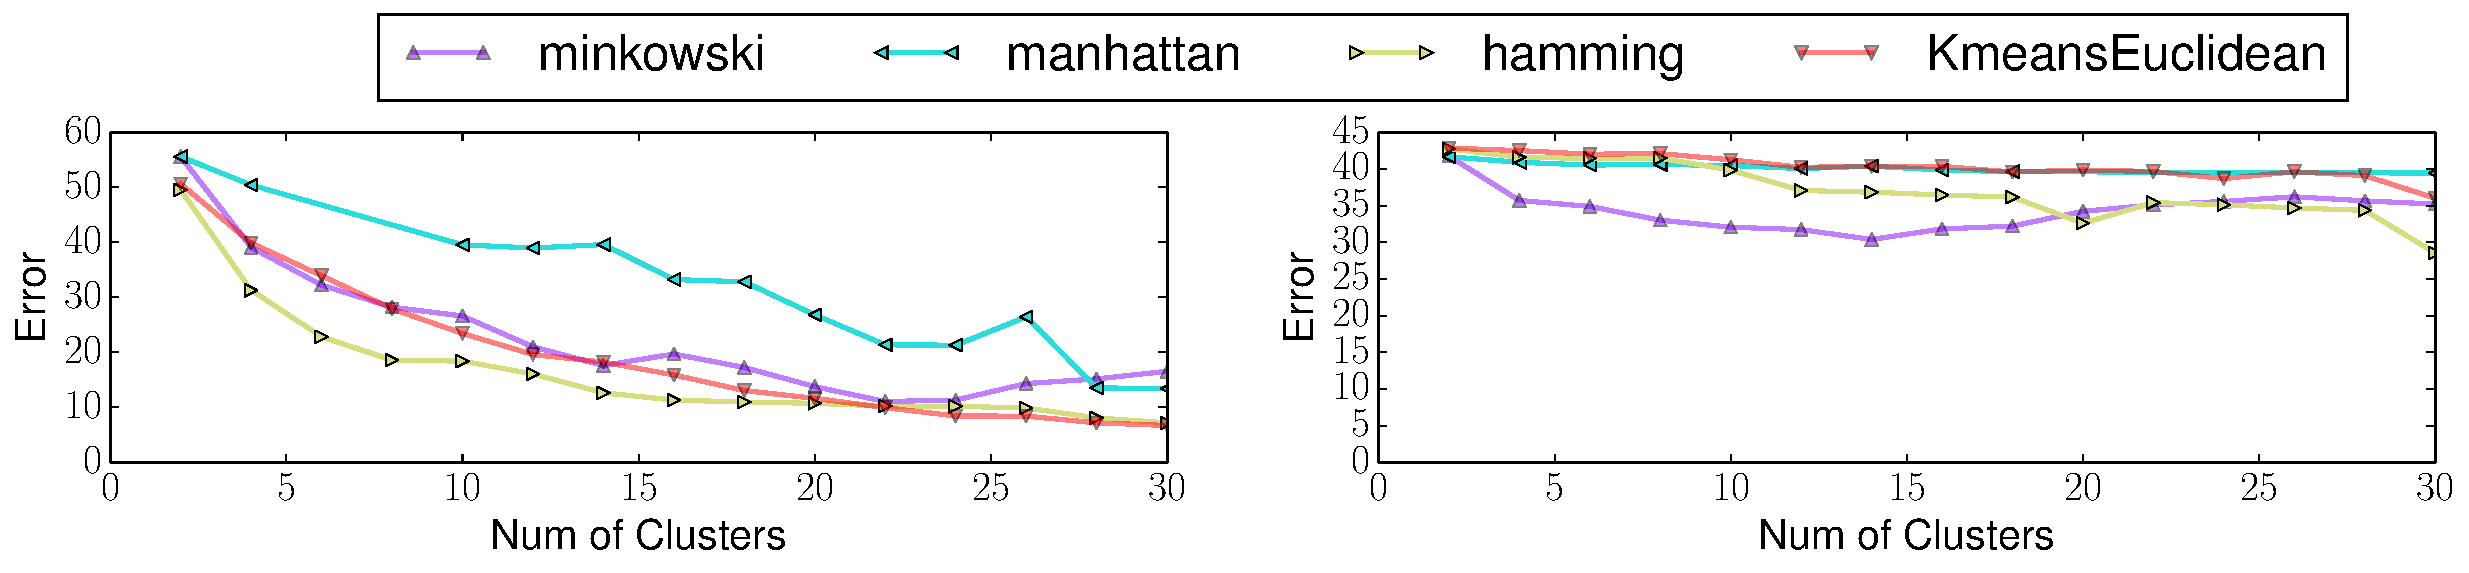
\includegraphics[width=1\textwidth]{QueryLogSummarization/graphics/ErrorVNumCluster.pdf}
 \bfcaption{Error v. Number of Clusters (Left: PocketData, Right: US Bank)}   
 \label{fig:ErrorVNumCluster}
\end{subfigure}
~
%\begin{subfigure}[b]{1\textwidth}
%    \centering      
%    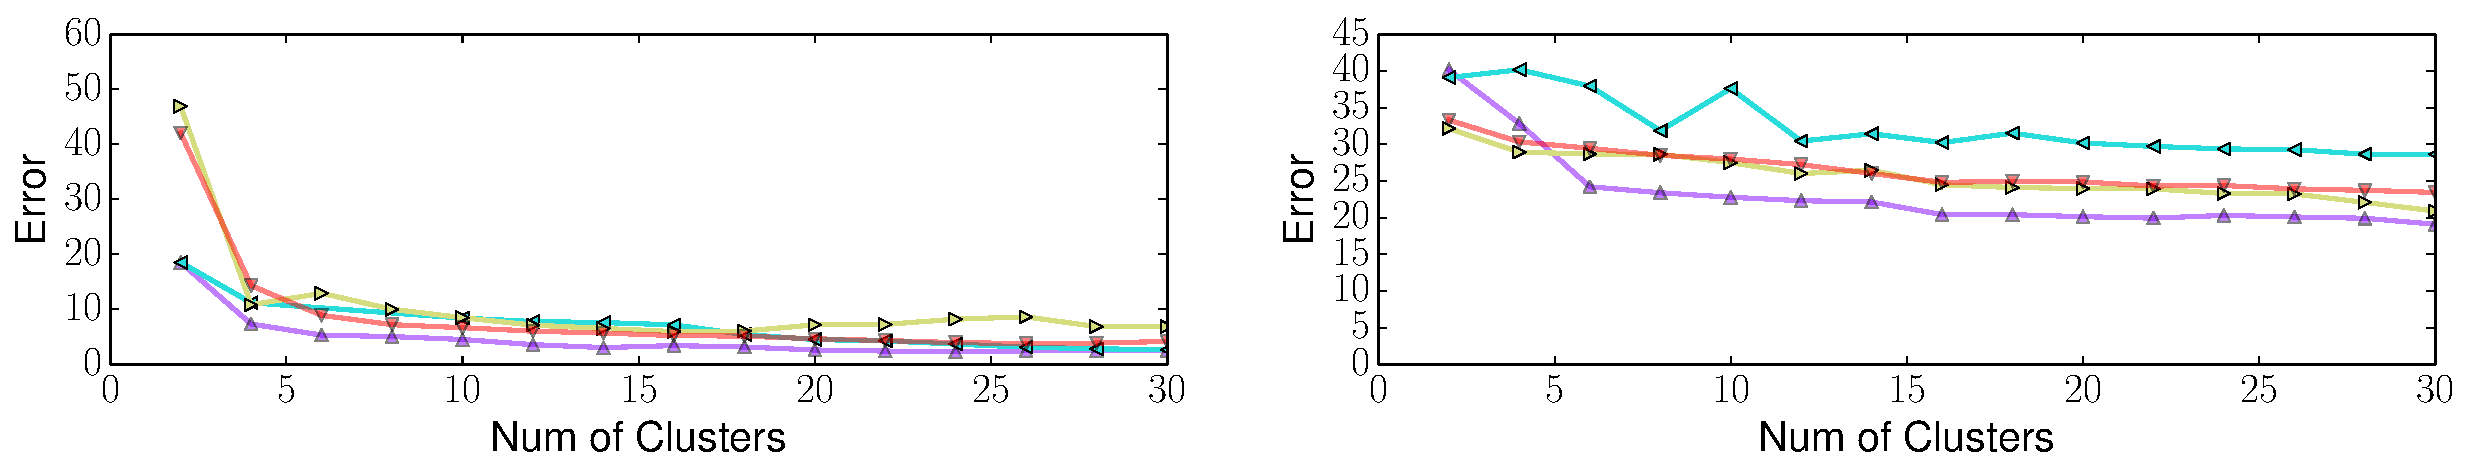
\includegraphics[width=1\textwidth]{QueryLogSummarization/graphics/MultiAdjustedErrorVNumCluster.pdf}
% \bfcaption{Error v. Number of Clusters under multiplicity-aware Clustering (Left: PocketData, Right: US Bank)}   
%\label{fig:MultiAdjustedErrorVNumCluster}
%\end{subfigure}
%~
\begin{subfigure}[b]{0.98\textwidth}
    \centering      
    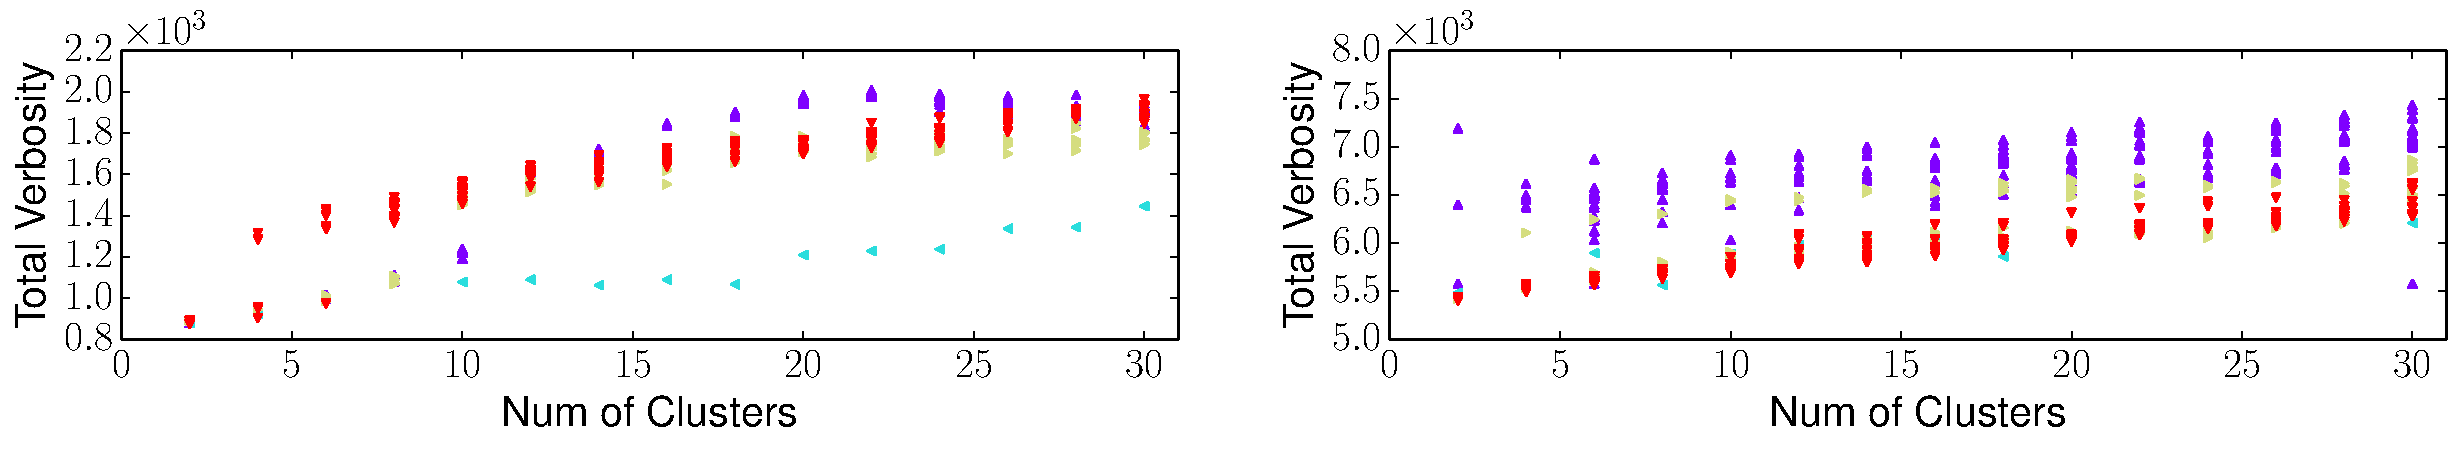
\includegraphics[width=1\textwidth]{QueryLogSummarization/graphics/TotalVerbosityVNumCluster.pdf}
 \bfcaption{Total Verbosity v. Number of Clusters (Left: PocketData, Right: US Bank); 
Each point is the verbosity of one of ten trials.  The Y-axis' lower bound is the verbosity at 1 cluster to better show the change in verbosity.}   
 \label{fig:TotalVerbosityVNumCluster}
\end{subfigure}
~
%\begin{subfigure}[b]{0.98\textwidth}
%    \centering      \includegraphics[width=1\textwidth]{QueryLogSummarization/graphics/ErrorVExpectationOfVerbosity.pdf}
% \bfcaption{Error v. Expectation of Verbosity (Left: PocketData, Right: US Bank)}   \label{fig:ErrorVExpectationOfVerbosity}
%\end{subfigure}
%~
\begin{subfigure}[b]{0.99\textwidth}
    \centering      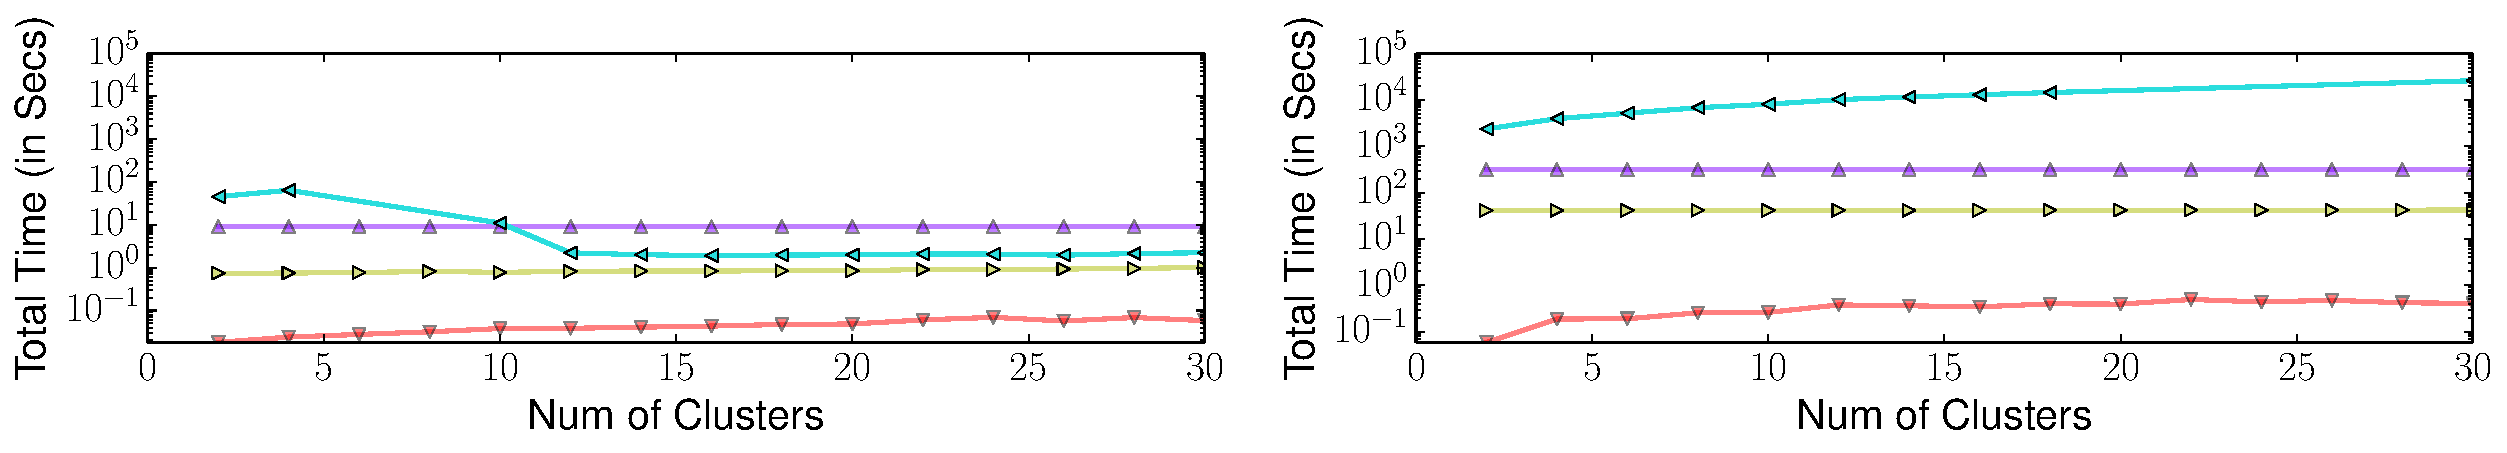
\includegraphics[width=1\textwidth]{QueryLogSummarization/graphics/RunningTimeVNumCluster.pdf}
 \bfcaption{Runtime v. Number of Clusters (Left: PocketData, Right: US Bank)}   \label{fig:RunningTimeVCluster}
\end{subfigure}
~
 \bfcaption{Clustering Schemes Comparison}
 \label{fig:distancemeasurecomparison} 
 \trimfigurewhitespace
\end{figure*}

\section{Pattern Mixture Compression}
\label{sec:constructingencodings}
We are now ready to describe the \systemnameone compression scheme.
Broadly, \systemnameone attempts to identify a pattern mixture encoding that optimizes for some target trade-off between Total Verbosity and Error.  
A naive --- though impractical --- approach to finding such an encoding would be to search the entire space of possible pattern mixture encodings.
Instead, \systemnameone approximates the same outcome by first identifying the naive mixture encoding that is closest to optimal for the desired trade-off.
As I will show experimentally, this naive mixture encoding is competitive with more complicated, slower techniques for summarizing query logs.
We also explore a hypothetical second stage, where \systemnameone refines the naive mixture encoding to further reduce Error.
The outcome of this hypothetical stage has a slightly lower Error and Verbosity, but does not admit efficient computation of database statistics. 

\subsection{Constructing Naive Mixture Encodings}
\label{sec:constructingnaivemixtureencodings}
\systemnameone searches for a naive mixture encoding that best optimizes for a requested tradeoff between Total Verbosity and Error.  
As a way to make this search efficient, we observe that a log (or log partition) uniquely determines its naive (or naive mixture) encoding. 
Thus the problem of searching for a naive mixture encoding reduces to searching for the corresponding log partitioning.
We further observe that the Error of a naive mixture encoding is proportional to the diversity of the queries in the log being encoded: 
The more uniform the log (or partition), the lower the Error.
Hence, the partitioning problem further reduces to clustering queries in the log by feature overlap.
 \begin{example}
 \label{example:twolevelnaivemixtureencoding}
 Figure~\ref{fig:hierarchicalnaivemixtureencoding} shows an example of constructing a naive mixture encoding from partitioning one cluster into two.
 The naive encodings on the child level (Figure~\ref{fig:childlevel}), each with lower Average Verbosity and Encoding Error, provide a cleaner view of the mixed workload.
 % The Average Verbosity of the resulting naive mixture encoding is lower, as is the generalized Encoding Error.
 However, note that feature \cqword{FROM}{Messages} appears in both children, so the Total Verbosity of the child level is one higher than the parent --- observers see the same feature twice.
 \end{example}
To identify a suitable clustering scheme, we next evaluate four commonly used clustering schemes with respect to their ability to create naive mixture encodings with low Error and Verbosity: (1) KMeans~\cite{DBLP:journals/prl/Jain10} with Euclidean distance (i.e., $l_2$-norm) and Spectral Clustering~\cite{DBLP:journals/jacm/KannanVV04} with (2) Manhattan (i.e., $l_1$-norm), (3) Minkowski (i.e., $l_p$-norm) with $p=4$, and (4) Hamming distances\footnote{Spectral Clustering with Euclidean, Chebyshev and Canberra distances are also evaluated; These did not perform better and I omit them in the interest of conciseness.}.
 \begin{figure}
  \centering
 \begin{subfigure}{\columnwidth}
   {\small
     \begin{tabular}{r|p{60mm}}
     \textbf{SELECT} & 
         \texttt{sms\_type},
         \textcolor{light-gray}{\texttt{external\_ids}},
         \texttt{\_time},
         \texttt{\_id}\\ \hline
     \textbf{FROM} &
         \texttt{Messages}\\ \hline
     \textbf{WHERE} &
         \texttt{(sms\_type=1)} $\wedge$
         \textcolor{mid-gray}{\texttt{(sms\_type=0)}} $\wedge$
         \texttt{(status=1)}   
         $\wedge$~\textcolor{light-gray}{\texttt{(\_time$\geq$14260)}} $\wedge$~\texttt{(transport=3)} 
     \end{tabular}
   }
   \bfcaption{\textit{Parent Level}: Naive encoding of a mixture of two workloads.}
   \label{fig:parentlevel}
 \end{subfigure}\\[2mm]
 \begin{subfigure}{\columnwidth}
 \hspace*{-1mm}
   {\small
     \centering
     \begin{tabular}{r|p{20mm}}
     \textbf{SELECT} & 
         \texttt{sms\_type},\texttt{\_time}
         \\ \hline
     \textbf{FROM} &
         \texttt{Messages}\\ \hline
     \textbf{WHERE} &
         \texttt{(sms\_type=1)}$\wedge$ 
         \textcolor{mid-gray}{\texttt{(sms\_type=0)}}$\wedge$
         \textcolor{light-gray}{\texttt{(\_time$\geq$14260)}}  
     \end{tabular}
     \begin{tabular}{r|p{20mm}}
     \textbf{SELECT} & 
         \texttt{\_id}, \textcolor{light-gray}{\texttt{external\_ids}}
         \\ \hline
     \textbf{FROM} &
         \texttt{Messages}\\ \hline
     \textbf{WHERE} &
         \texttt{(status=1)}$\wedge$
         \texttt{(transport=3)} 
     \end{tabular}
   }
   \bfcaption{\textit{Child Level}: Two children encodings that separately summarize each workload.}
   \label{fig:childlevel}  
 \end{subfigure}\\[2mm]
 \bfcaption{\textbf{Constructing a naive mixture encoding}}
 \label{fig:hierarchicalnaivemixtureencoding}
 \trimfigurewhitespace
 \end{figure}

\tinysection{Experiment Setup}
Spectral and KMeans clustering algorithms are implemented by \textit{sklearn}~\cite{scikit-learn} in Python. 
We gradually increase $K$ (i.e., the number of clusters) for each clustering scheme to mimic the process of continuously sub-clustering the log, tolerating higher Total Verbosity for lower Error.
To reduce randomness in clustering, we run each of them $10$ times for each $K$ and averaging the Error of the resulting encodings.  
We use two datasets: ``US Bank'' and ``PocketData''.  
Both datsets and the data preparation process are described in detail in Section~\ref{sec:commonexperimentsettings}. 
All results for our clustering experiments are shown in Figure~\ref{fig:distancemeasurecomparison}.

\subsubsection{Clustering}
\label{sec:clustering}
I next show that clustering is an effective way to consistently reduce Error, although no one clustering scheme is ideal for all three of Error, Verbosity, and runtime.

\tinysection{More clusters reduces Error}
Figure~\ref{fig:ErrorVNumCluster} compares the relationship between the number of clusters (x-axis) and Error (y-axis), showing the varying rates of convergence to zero Error for each clustering scheme.
We observe that adding more clusters does consistently reduce Error for both data sets, regardless of clustering algorithm or distance measure.
We note that the US Bank dataset is significantly more diverse than the PocketData dataset, with respect to the total number of features (See Table~\ref{table:datasummary}) and that more than $30$ clusters may be required for reaching near-zero Error.
In general, Hamming distance converges faster than other distance measures on PocketData.
Minkowski distance shows faster convergence rate than Hamming within $14$ clusters on the US bank dataset. 

\tinysection{Adding more clusters increases Verbosity}
Figure~\ref{fig:TotalVerbosityVNumCluster} compares the relationship between the number of clusters (x-axis) and Verbosity (y-axis).
We observe that Verbosity increases with the number of clusters.
This is because when a partition is split, each feature common to both partitions increases the Verbosity by one (as shown in Example~\ref{example:twolevelnaivemixtureencoding}).

\tinysection{Hierarchical Clustering}
The clustering schemes produce non-monotonic cluster assignments. That is, Error can occasionally grow as clusters are added (Figure~\ref{fig:ErrorVNumCluster}). 
An alternative is to use hierarchical clustering~\cite{DBLP:journals/prl/Jain10}, which forces monotonic assignments and offers more dynamic control over the Error/Verbosity tradeoff.

\tinysection{Run Time Comparison}
The total runtime (y-axis) in Figure~\ref{fig:RunningTimeVCluster} includes both distance matrix computation time (if any) and clustering time. 
Note the log-scale: K-Means is orders of magnitude faster than the others.

\tinysection{Take-Aways}
For time-sensitive applications, KMeans algorithm is preferred to Spectral Clustering.
With respect to distance measures, minkowski (i.e., $l_p$-norm) with $p=4$ provides the best tradeoff between Error and runtime.

\tinysection{Visualizing Naive Mixture Encoding}
As with normal pattern summaries, naive mixture summaries are also interpretable.
For example a visualization like that of Figure~\ref{fig:screenshots:nocorrelation} can be repeated, once for each cluster.  
For more details, see our accompanying technical report~\cite{DBLP:journals/corr/abs-1809-00405}.

\subsection{Approximating Log Statistics}
Recall that our primary goal is estimating frequencies.
In particular, we are interested in counting the occurrences $\Gamma_\pattern(L)$ (i.e., $p(Q\supseteq\vec b)\cdot |L|$) of some pattern $\pattern$ in the log.
%$$\Gamma_\pattern(L) = |\comprehension{\vec q}{\vec q \in L \wedge \pattern \subseteq \vec q}|$$
Recall that a naive encoding $\naiveencoding$ includes only single-feature patterns (i.e., patterns exactly encoding $p(X_i\ge x_i)$) and that the closed-form representation for the maximum entropy distribution $\overline \rho_{\naiveencoding}$ arises by independence between features (i.e., $\overline \rho_{\naiveencoding}(Q = \vec q) = \prod_{i} p(X_i = x_i)$).
Similarly, we use the independence assumption to estimate:
$$est[\Gamma_\pattern(L)\;|\;\naiveencoding]=\overline \rho_{\naiveencoding}(Q \supseteq \vec b)\cdot |L| = \prod_{i} p(X_i \geq x_i)\cdot |L|$$

This process trivially generalizes to naive pattern mixture encodings by mixing distributions.  
Specifically, given a set of partitions $L_1 \cup \ldots \cup L_K = L$, the estimated counts for $\Gamma_\pattern(L)$ under each individual partition $L_i$ can be computed based on the partition's naive encoding $\naiveencoding_i$, and we then sum up the estimated counts in each partition:
$$est[\;\Gamma_\pattern(L_i)\;|\;\naiveencoding_1, \ldots, \naiveencoding_K\;] = \sum_{i \in [1, K]} est[\;\Gamma_\pattern(L_i)\;|\;\naiveencoding_i\;]$$

\begin{figure*}[h!]
\captionsetup[subfigure]{justification=centering}
    \centering 
    
\begin{subfigure}[b]{0.48\textwidth}
    \centering     
     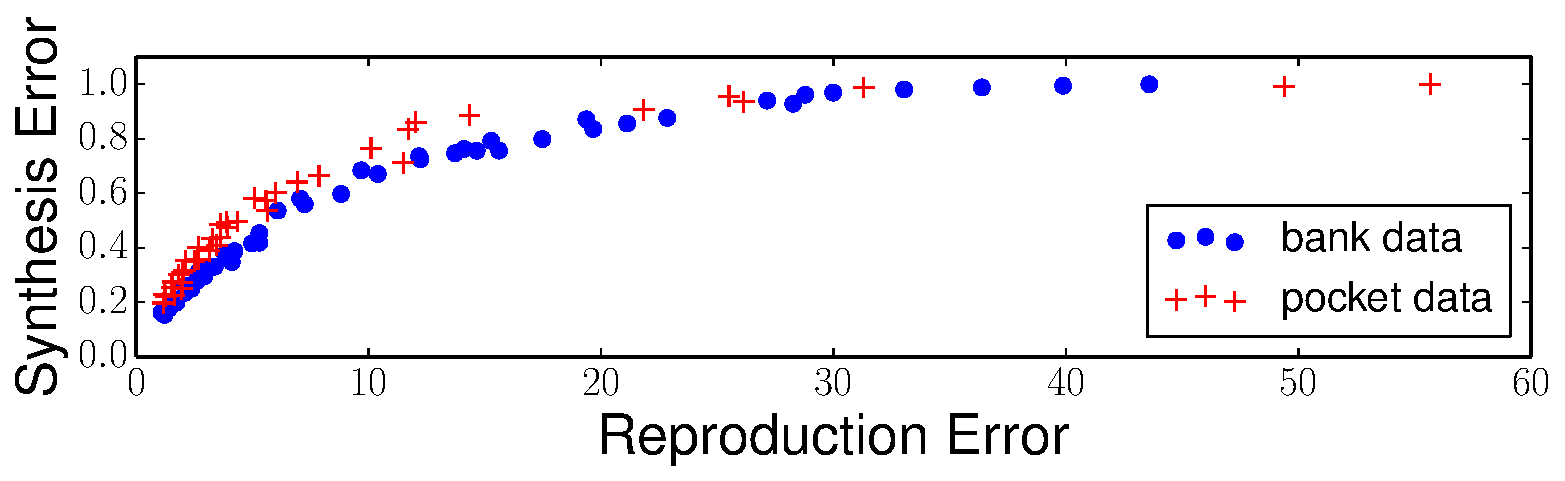
\includegraphics[width=1\textwidth]{QueryLogSummarization/graphics/synthesis_error.pdf}
 \bfcaption{Synthesis Error v. \Errorname}   
 \label{fig:synthesis_error_versus_reproduction_error}
\end{subfigure}
~
\begin{subfigure}[b]{0.48\textwidth}
    \centering      
    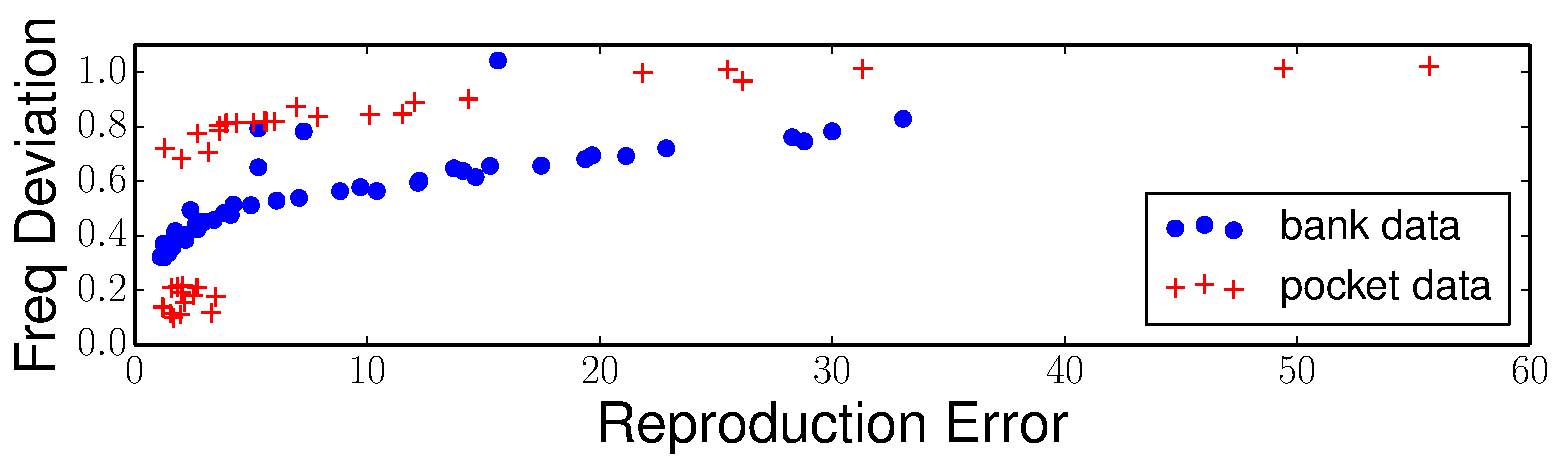
\includegraphics[width=1\textwidth]{QueryLogSummarization/graphics/marginal_deviation.pdf}
 \bfcaption{Frequency Deviation v. \Errorname}   
 \label{fig:marginal_deviation_versus_reproduction_error}
\end{subfigure}

 \bfcaption{Effectiveness of Naive Mixture Encoding}
 \label{fig:effectiveness_of_naive_mixture_encoding} 
 \trimfigurewhitespace
\end{figure*} 

\subsection{Pattern Synthesis \& Frequency Estimate}
In this section, we empirically verify the effectiveness of naive mixture encodings in approximating log statistics from two related perspectives. 
The first perspective focuses on \textit{synthesis error}. 
It measures whether patterns synthesized by the naive mixture encoding actually appear in the log.
From the second perspective, we further investigate the \textit{frequency deviation} of patterns contained in the log.
This evaluates whether a naive mixture encoding computes the correct frequency for patterns of interest to client applications.
Experimental results are shown in Figure~\ref{fig:effectiveness_of_naive_mixture_encoding}.
Both synthesis error and frequency deviation consistently decrease given more clusters.
Furthermore, as we vary the number of clusters, both measures correlate with \errorname.

\noindent \textbf{Synthesis Error}
is measured by $1-\frac{m}{n}$ where $m$ out of $n$ randomly synthesized patterns actually appear in the log.
Intuitively, when synthesis error grows, it is more likely that a pattern from the synthesized log will not appear in the original log (i.e., smaller values are better).
Figure~\ref{fig:synthesis_error_versus_reproduction_error} shows synthesis error (y-axis) versus \errorname (x-axis).
The figure is generated by synthesizing $n=10000$ patterns from each cluster of the log.
Note that different values of $n$ give similar observations.
The overall synthesis error is measured by the average of synthesis errors for all clusters, weighted by the proportion of queries in each cluster.

\noindent \textbf{Frequency Deviation}
is measured for a pattern by $\frac{|est-t|}{t}$ where $t$ stands for true frequency of a pattern and $est$ is the one estimated by the naive mixture encoding.
Since frequency deviation is smaller when evaluated on a pattern contained in the other, as an alternative, we treat each distinct query in the log as a pattern and the frequency deviation on it will be the worst case for all patterns that it contains.
Intuitively, this value captures the percentage error of frequency estimates (i.e., smaller values are better).
For each cluster, we sum frequency deviations on all of its distinct queries and the final frequency deviation for the whole log is an weighted average (same as synthesis error) over all clusters.
Figure~\ref{fig:marginal_deviation_versus_reproduction_error} shows frequency deviation (y-axis) versus \errorname (x-axis).

\subsection{Naive Encoding Refinement}
\label{sec:naivemixtureencodingrefinement}
Naive mixture encodings can already achieve close to near-zero Error (Figure~\ref{fig:ErrorVNumCluster}), have low Total Verbosity, and admit efficiently computable log statistics $\Gamma_\pattern(L)$.
Doing so makes estimating statistics more computationally expensive.
However, as a thought experiment we consider a hypothetical second pass to enrich naive mixture encodings with non-naive patterns.
We start by considering the simpler problem of identifying the \emph{individual} non-naive pattern that maximally reduces the \errorname of a naive encoding.

\tinysection{Feature-Correlation Refinement}
Recall that under naive encodings, we have a closed-form estimation $\overline \rho_{\naiveencoding}(Q \supseteq \vec b)$ of pattern frequencies $p(Q\supseteq\vec b)$.
We thus define the \textit{feature-correlation} of pattern $\vec b$ as the log-difference from its actual frequency to the estimate.
$$fc(\vec b, \naiveencoding) = |\log\left(
    p(Q \supseteq \vec b)
\right) - \log\left(
  %\prod_{i} p(X_i \geq x_i)
  \overline \rho_{\naiveencoding}(Q \supseteq \vec b)
\right)|$$
Intuitively, patterns with higher feature correlations carry more information content of the log that its naive encoding ignores, making them ideal candidates for addition to the naive encoding.
For two patterns with the same feature-correlation, the one that occurs more frequently~\cite{DBLP:journals/datamine/HanCXY07} will have greater impact on \errorname. 
As a result, we compute an overall score for ranking individual patterns:  
$$corr\_rank(\vec{b})=p(Q \supseteq \vec b) \cdot fc(\vec b, \naiveencoding)$$
I will show in Section~\ref{sec:motivateencodingerror} that $corr\_rank$ closely correlates with \errorname.
That is, a higher $corr\_rank$ value indicates that a pattern produces a greater reduction in \errorname if introduced into the naive encoding.

\tinysection{Pattern Diversification}
In general, we would like to identify a \emph{set} of patterns.
The greedy approach that adds patterns one by one based on their ranking scores $corr\_rank$ is unreliable, as modifying the naive encoding invalidates the closed-form estimation $\overline \rho_{\naiveencoding}(Q \supseteq \vec b)$ that score $corr\_rank$ relies on.
In other words, we can not sum up $corr\_rank$ scores of patterns in a set in order to rank its overall contribution to \errorname reduction, as information content carried by patterns may overlap.
To counter such overlap, or equivalently to \textit{diversify} patterns, a search through the space of pattern-sets is needed.
This type of diversification is commonly used in pattern mining applications, but can quickly become expensive.
As I show experimentally in Section~\ref{sec:motivatepatternmixturesummaries}, the benefit of diversification is minimal.





\section{Experiments}
\label{sec:experiments}
In this section, we design experiments to empirically (1) validate that \errorname correlates with Deviation and (2)~evaluate the effectiveness of \systemnameone compression.

We use two specific datasets in the experiment: (1) SQL query logs of the Google+ Android app extracted from the PocketData public dataset~\cite{DBLP:conf/tpctc/KennedyACZ15} and (2) SQL query logs that capture all query activity on the majority of databases at a major US bank over a period of approximately 19 hours.
A summary of these two datasets is given in Table~\ref{table:datasummary}.

\begin{table}
\centering
\bfcaption{Summary of Data sets}
\label{table:datasummary}
{\small \centering
\begin{tabular}{c c c}
\toprule
Statistics & PocketData & US bank \\
\midrule
\# Queries & 629582& 1244243\\
\midrule
\# Distinct queries & 605& 188184\\
\midrule
\# Distinct queries (w/o const)& 605& 1712\\
\midrule
\# Distinct conjunctive queries & 135& 1494\\
\midrule
\# Distinct re-writable queries & 605& 1712\\
\midrule
Max query multiplicity & 48651 & 208742\\
\midrule
\# Distinct features & 863& 144708\\
\midrule
\# Distinct features (w/o const) & 863& 5290\\
\midrule
Average features per query & 14.78& 16.56\\
\bottomrule
\end{tabular}
}
\trimfigurewhitespace
\end{table}

\begin{figure*}[h!]
	\captionsetup[subfigure]{justification=centering}
    \centering
    \begin{subfigure}[b]{0.48\textwidth}
        \centering
        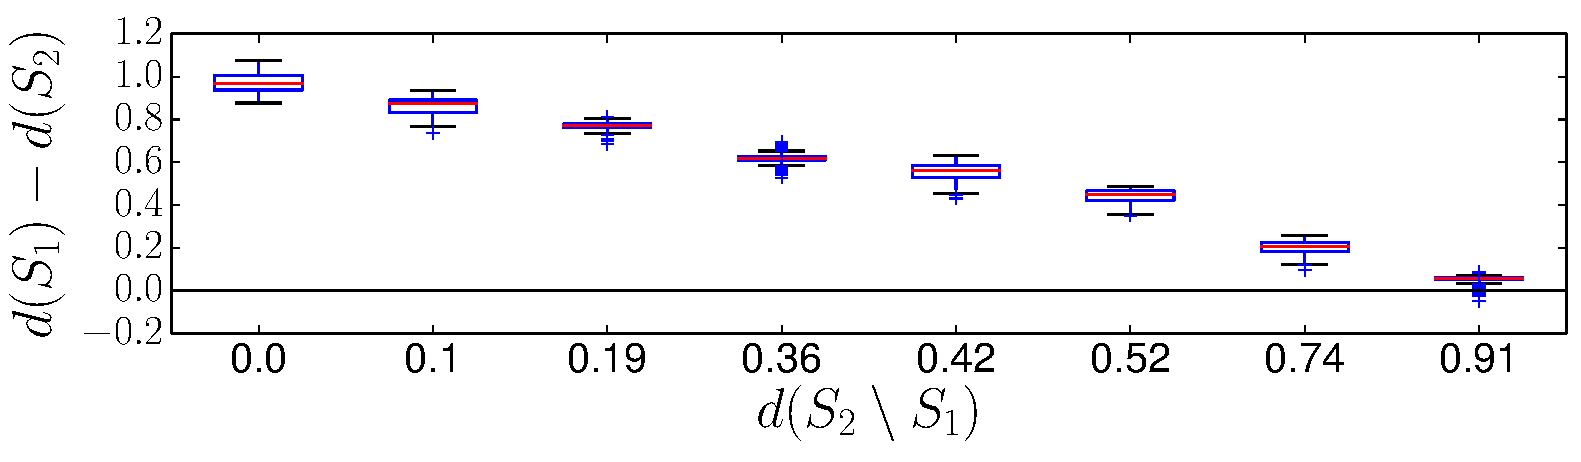
\includegraphics[width=\textwidth]{QueryLogSummarization/graphics/ContainmentCapturesDeviation_BankData.pdf}
        \bfcaption{Containment captures Deviation (US bank)}
        \label{fig:containmentcapturesdeviation_bankdata}
    \end{subfigure}
        ~
    \begin{subfigure}[b]{0.48\textwidth}
        \centering
        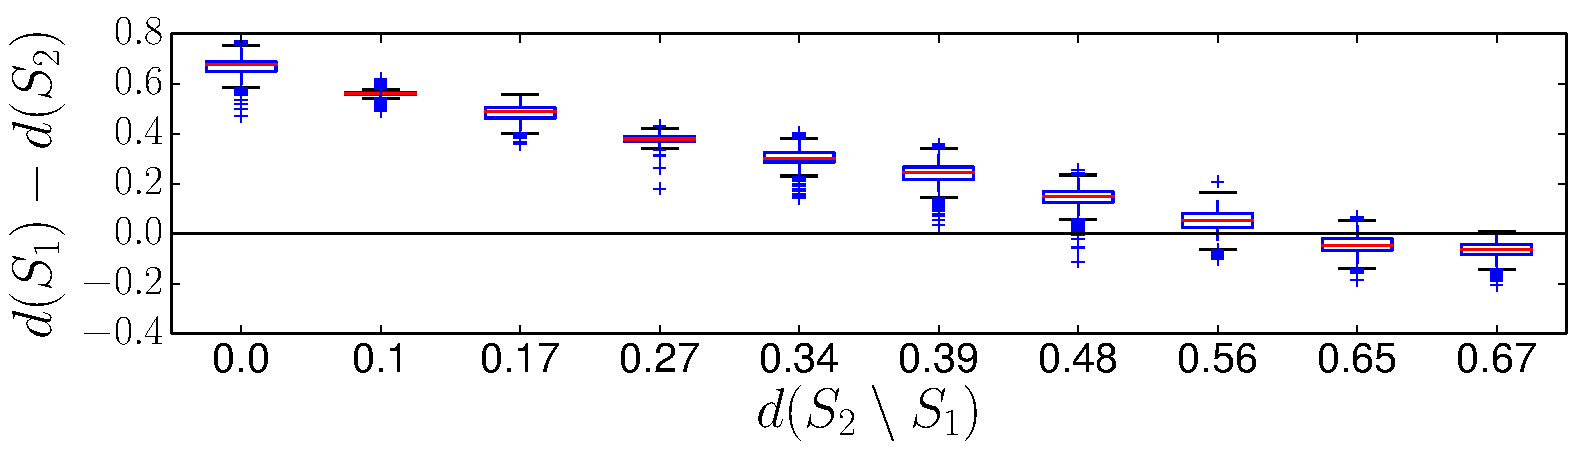
\includegraphics[width=\textwidth]{QueryLogSummarization/graphics/ContainmentCapturesDeviation_PocketData.pdf}
        \bfcaption{Containment captures Deviation (PocketData)}
        \label{fig:containmentcapturesdeviation_pocketdata}
    \end{subfigure}
    ~
    \begin{subfigure}[b]{0.485\textwidth}
        \centering
         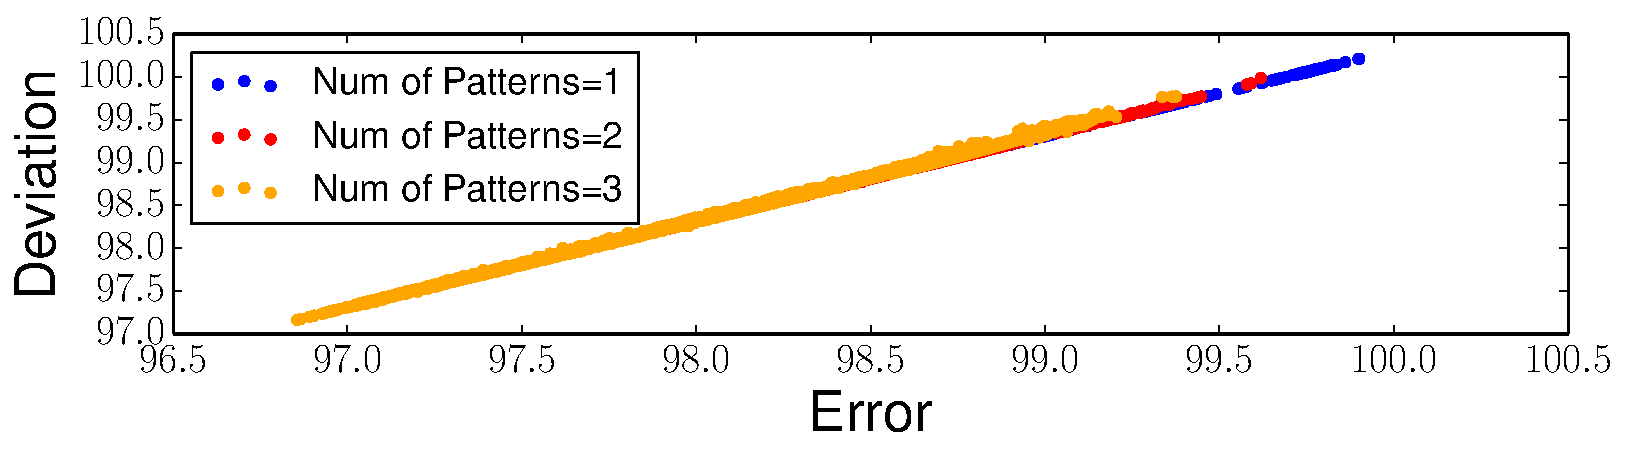
\includegraphics[width=\textwidth]{QueryLogSummarization/graphics/ErrorCapturesDeviation_BankData.pdf}
        \bfcaption{Error captures Deviation (US bank)}
        \label{fig:errorcapturesdeviation_bankdata}
    \end{subfigure}
        ~
    \begin{subfigure}[b]{0.485\textwidth}
        \centering
        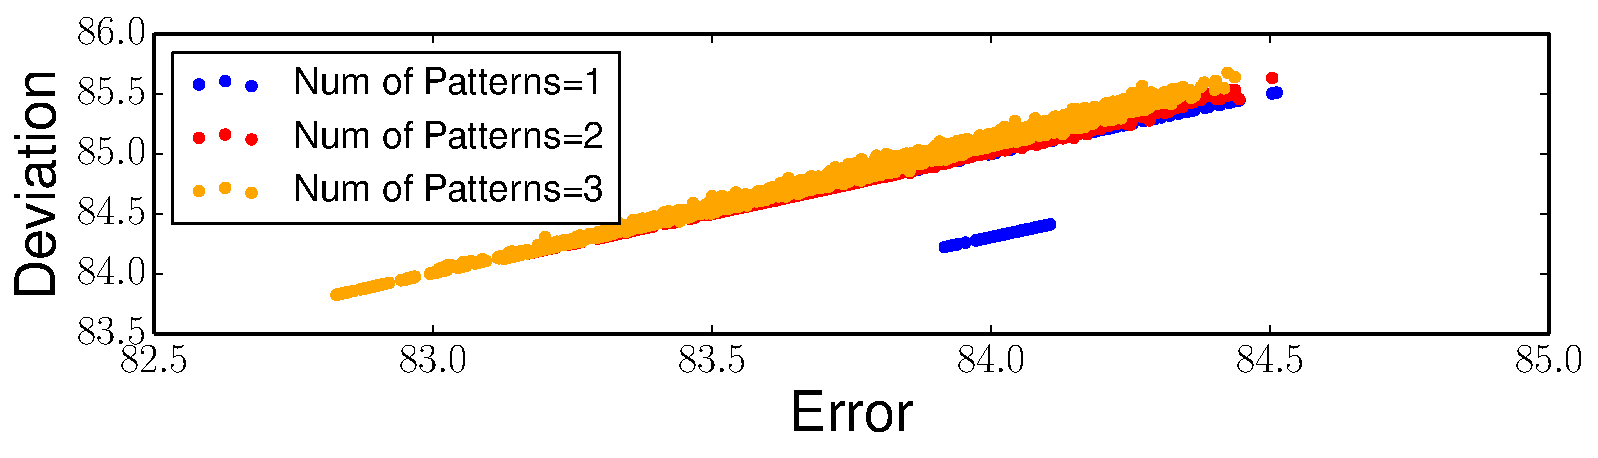
\includegraphics[width=\textwidth]{QueryLogSummarization/graphics/ErrorCapturesDeviation_PocketData.pdf}
        \bfcaption{Error captures Deviation (PocketData)}
        \label{fig:errorcapturesdeviation_pocketdata}
    \end{subfigure}
    ~
     \begin{subfigure}[b]{0.45\textwidth}
        \centering
        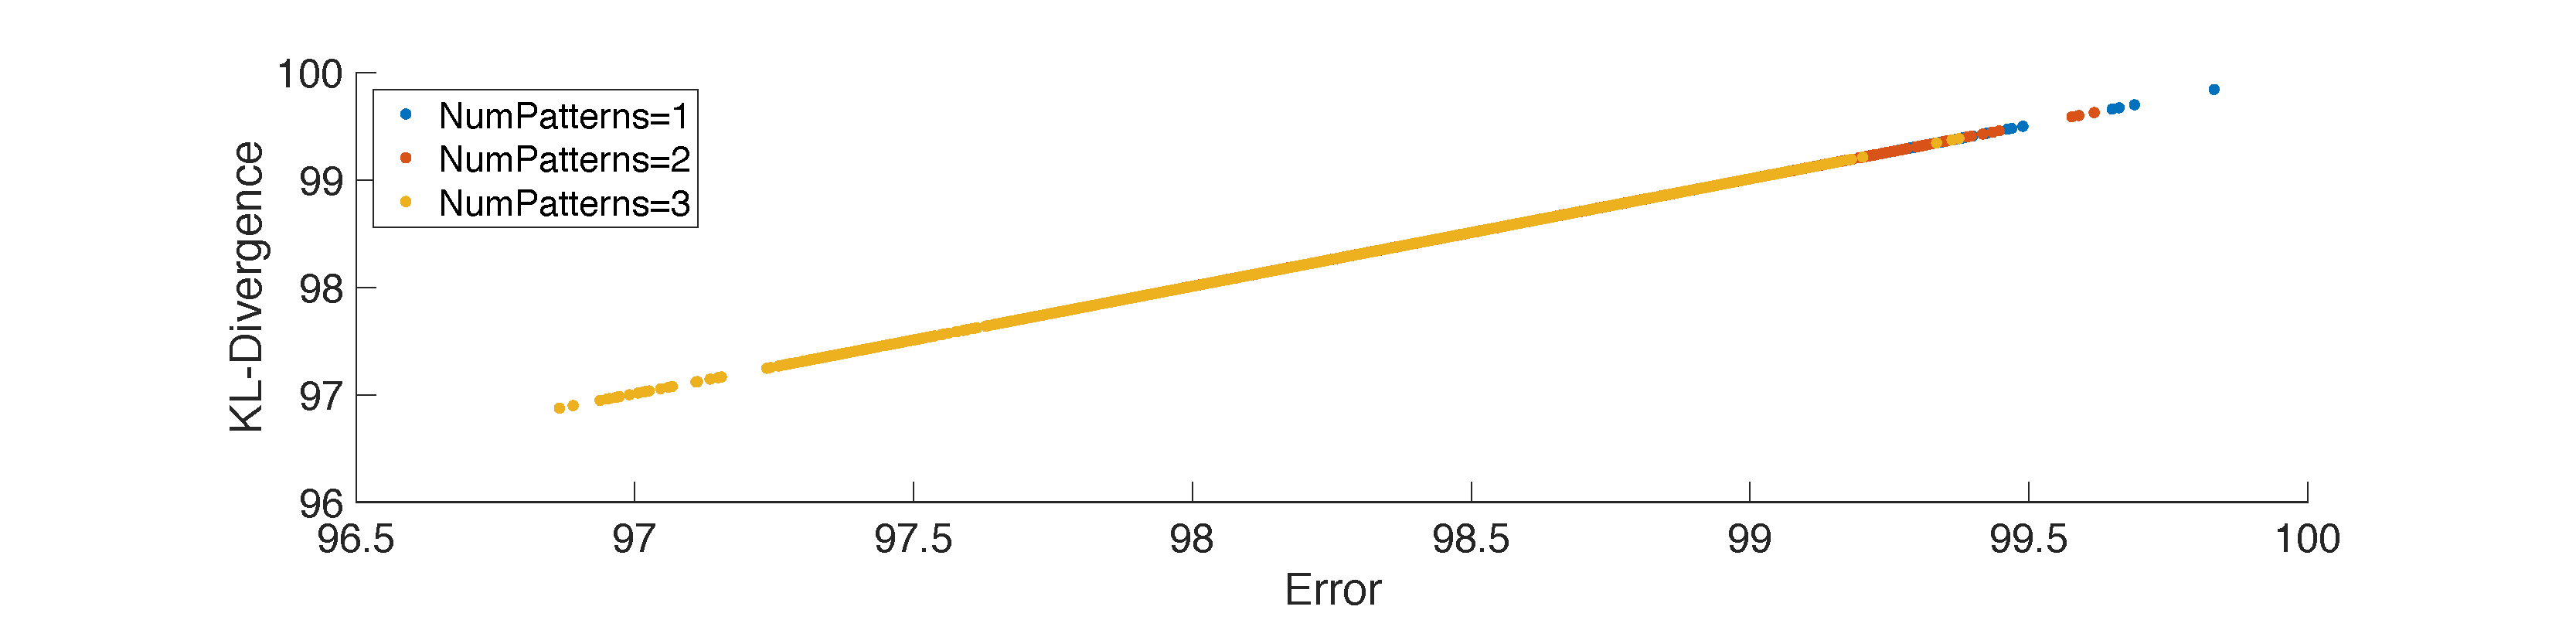
\includegraphics[width=\textwidth]{QueryLogSummarization/graphics/ErrorCapturesKL_BankData.pdf}
        \bfcaption{Error captures KL-divergence (US bank)}
        \label{fig:errorcapturesKL_bankdata}
\end{subfigure}
    ~
     \begin{subfigure}[b]{0.45\textwidth}
        \centering
        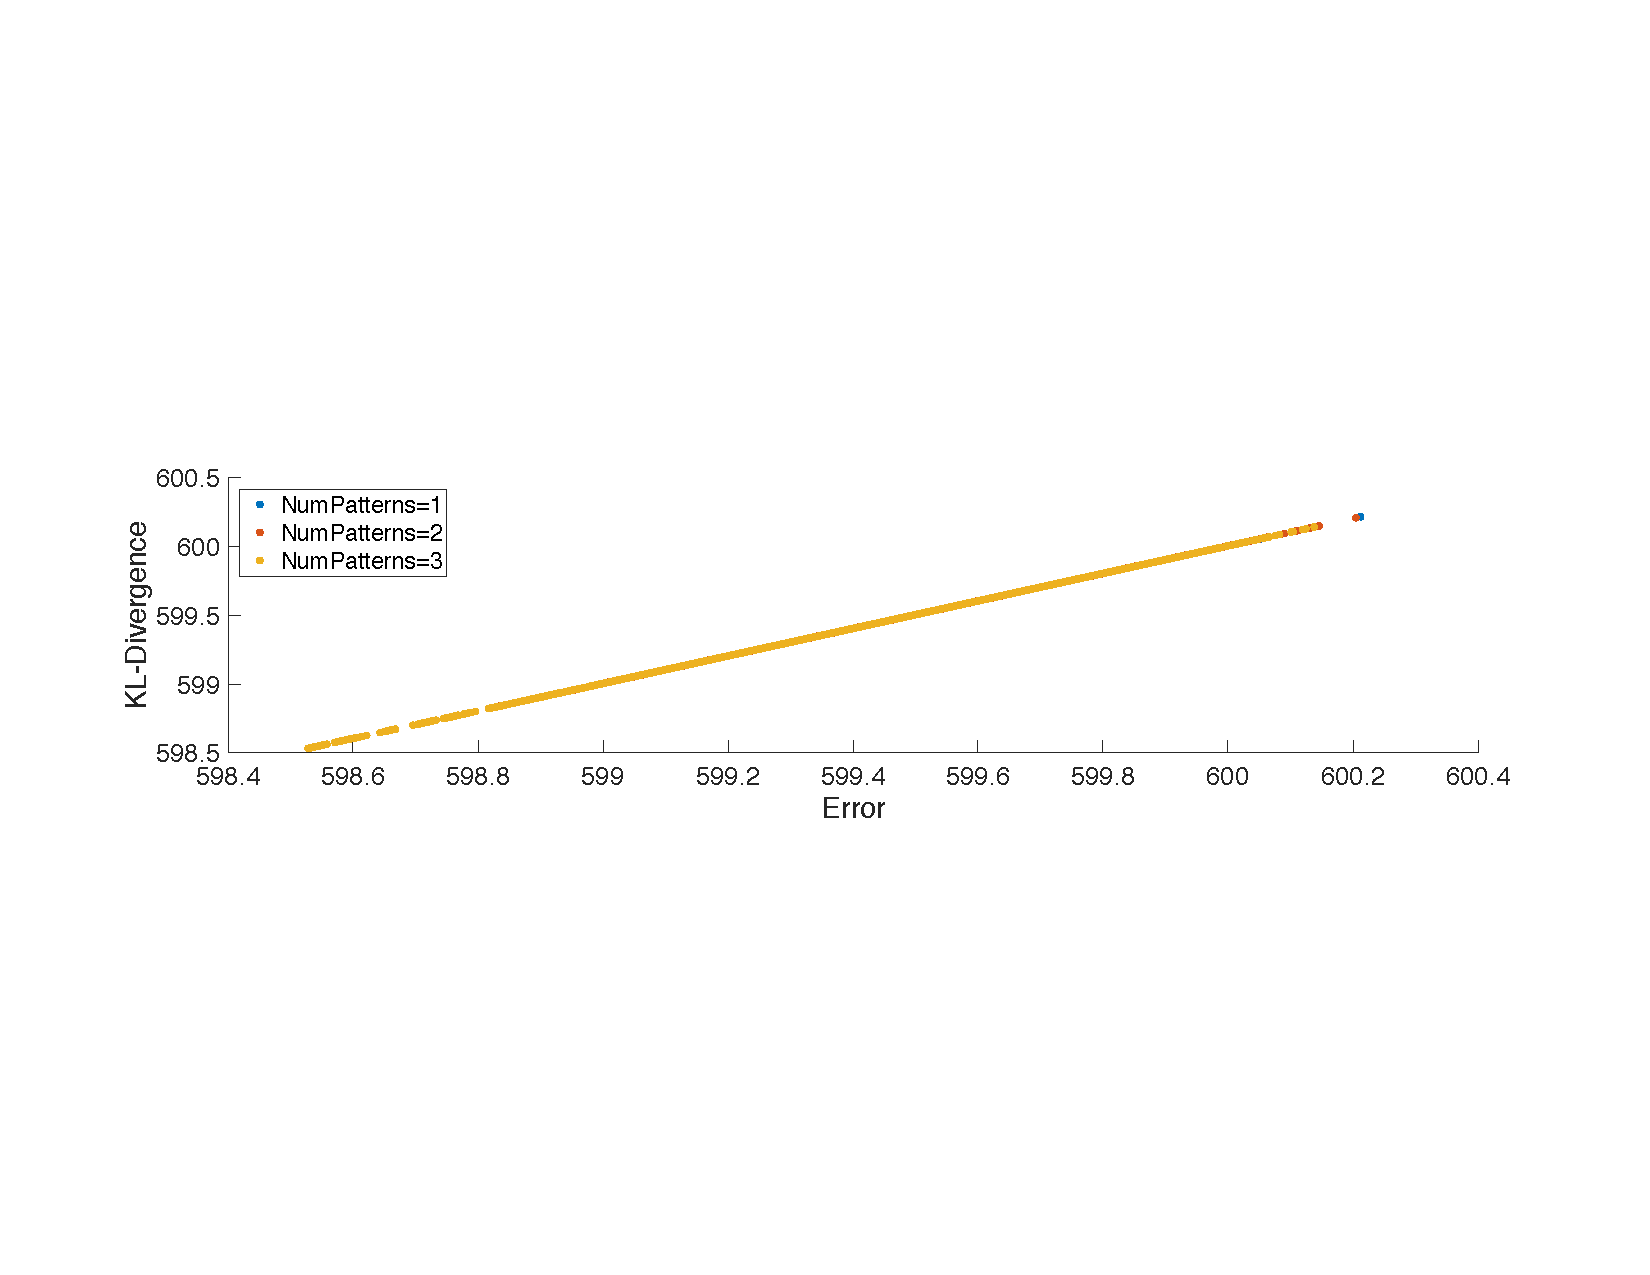
\includegraphics[width=\textwidth]{QueryLogSummarization/graphics/ErrorCapturesKL_PocketData.pdf}
        \bfcaption{Error captures KL-divergence (PocketData)}
        \label{fig:errorcapturesKL_pocketdata}
\end{subfigure}
    ~
     \begin{subfigure}[b]{0.48\textwidth}
        \centering     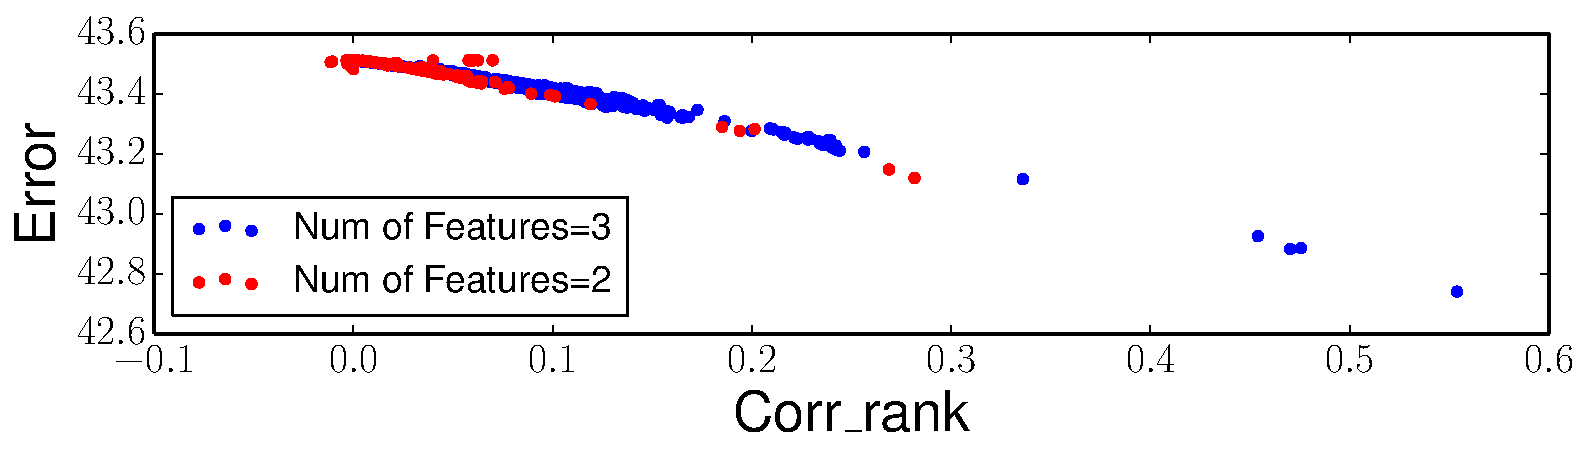
\includegraphics[width=\textwidth]{QueryLogSummarization/graphics/ErrorCapturesCorrelation_BankData.pdf}
        \bfcaption{Error captures Correlation (US bank)}
        \label{fig:errorcapturescorrelation_bankdata}
\end{subfigure}
    ~
     \begin{subfigure}[b]{0.48\textwidth}
        \centering     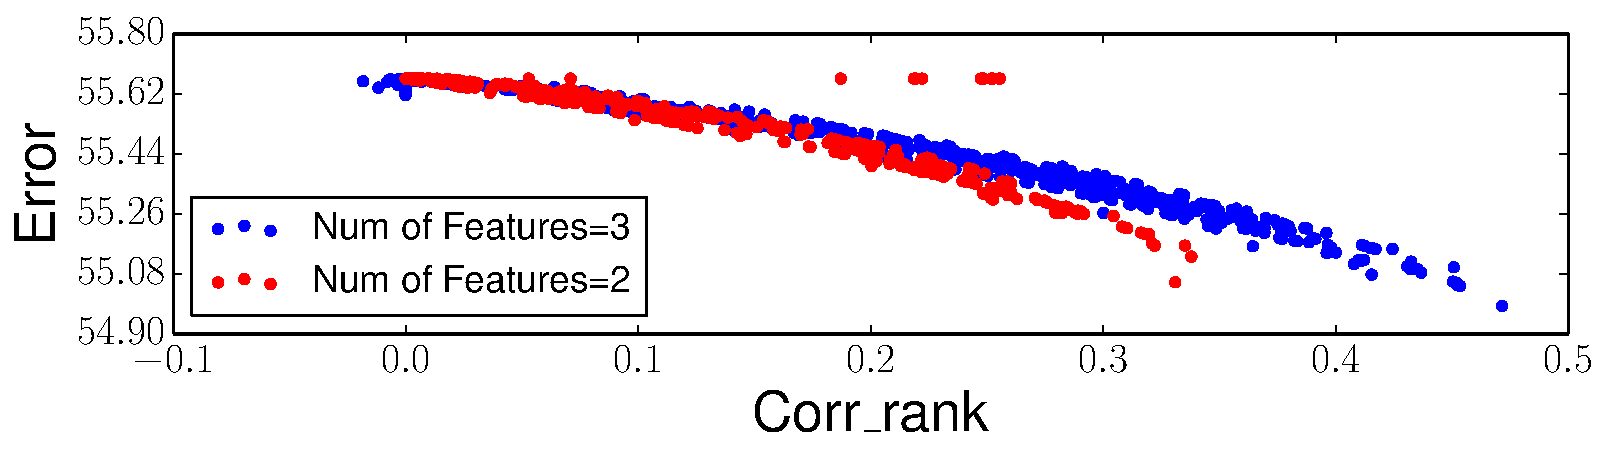
\includegraphics[width=\textwidth]{QueryLogSummarization/graphics/ErrorCapturesCorrelation_PocketData.pdf}
        \bfcaption{Error captures Correlation (PocketData)}
        \label{fig:errorcapturescorrelation_pocketdata}
\end{subfigure}
    
\bfcaption{Validating \Errorname}
\label{fig:validatingencodingerror}
\trimfigurewhitespace
\end{figure*}

\tinysection{The PocketData-Google+ query log} 
The dataset consists of SQL logs that capture all database activities of 11 Android phones. 
I selected the Google+ application for our study since it is one of the few applications where all users created a workload. 
This dataset is a stable workload of exclusively machine-generated queries.

\tinysection{The US bank query log}
This log is an anonymized record of queries processed by multiple relational database servers at a major US bank~\cite{DBLP:conf/www/KulLXCCKU16} over a period of 19 hours.
Of the nearly 73 million database operations captured, 58 million are not directly queries, but rather invocations of stored procedures.
A further 13 million used non-standard SQL features not supported by our SQL parser. 
Of the remaining of the 2.3 million parsed SQL queries, I base the analysis on the 1.25 million conjunctive \texttt{SELECT} queries. 
This dataset can be characterized as a diverse workload of both machine- and human-generated queries.

\tinysection{Common Experiment Settings}
\label{sec:commonexperimentsettings}
Experiments were performed on a 2.8 GHz Intel Core i7 CPU with 16 GB 1600 MHz DDR3 memory and a SSD running macOS Sierra.

\tinysection{Constant Removal}
A number of queries in the US bank query log differ only in hard-coded constant values.
Table~\ref{table:datasummary} shows the total number of queries, as well as the number of distinct queries if we ignore constants.
By comparison, queries in PocketData all use JDBC parameters.
For these experiments, we ignore constant values in queries.

\tinysection{Query Regularization}
We apply query rewrite rules (same as \cite{8352666}) to regularize queries into equivalent conjunctive forms, where possible. 
Table~\ref{table:datasummary} shows that $\frac{135}{605}$ and $\frac{1494}{1712}$ of distinct queries are in conjunctive form for PocketData and US bank respectively. 
After regularization, all queries in both data sets can be either simplified into conjunctive queries or re-written into a \texttt{UNION} of conjunctive queries compatible with feature scheme of Aligon et al.~\cite{DBLP:journals/kais/AligonGMRT14}.

\tinysection{Convex Optimization Solving}
All convex optimization problems for measuring \errorname and Deviation are solved by the \textit{successive approximation heuristic} implemented by the CVX toolbox~\cite{cvx} with the Sedumi solver.

\subsection{Validating \Errorname}
\label{sec:motivateencodingerror}
In this section, we validate that \errorname is a practical alternative to Deviation.
In addition, I also offer measurements on its correlation with Deviation and score $corr\_rank$ in Section~\ref{sec:naivemixtureencodingrefinement}.
%
As it is impractical to enumerate all possible encodings, I choose a subset of encodings for both datasets. 
Specifically, I first select all features with frequencies in the range $[0.01,0.99]$ and use these features to construct patterns.
I then enumerate combinations of $K$ (up to 3) patterns as our chosen encodings.

\tinysection{Containment Captures Deviation}
Here we empirically verify that containment (Section~\ref{sec:validateencodingerror}) captures Deviation (i.e., $\encoding_1\leq_{\Omega} \encoding_2\to d(\encoding_1)\leq d(\encoding_2)$) to complete the chain of reasoning that \errorname captures Deviation.
Figures~\ref{fig:containmentcapturesdeviation_bankdata} and \ref{fig:containmentcapturesdeviation_pocketdata} show all pairs of encodings where $\encoding_2\supset \encoding_1$.
The y-axis shows the difference in Deviation values (i.e., $d(\encoding_2)-d(\encoding_1)$).
Deviation $d(\encoding)$ is approximated by drawing 1 million samples from the space $\Omega_{\encoding}$ induced by the encoding $\encoding$.
For clarity, I bin pairs of encodings by the degree of overlap between them, measured by the Deviation of the set-difference $d(\encoding_2\setminus \encoding_1)$; Higher $d(\encoding_2\setminus \encoding_1)$ implies less overlap. 
Y-axis values are grouped into bins and visualized by boxplot where the boxes represent ranges within standard deviation and crosses are outliers.
Intuitively, \emph{points above zero} on the y-axis (i.e., $d(\encoding_2)-d(\encoding_1) > 0$) are pairs of encodings where the Deviation order agrees with containment order.
This is the case for virtually all encoding pairs.  

\tinysection{Additive Separability of Deviation}
We also observe from Figures~\ref{fig:containmentcapturesdeviation_bankdata} and ~\ref{fig:containmentcapturesdeviation_pocketdata} that agreement between Deviation and containment order is correlated with overlap: More similar encodings are more likely to have agreement.
Combined with Proposition~\ref{prop:monotone}, this shows first that for similar encodings, \errorname is likely to be a reliable indicator of Deviation.
This also suggests that Deviation is additively separable: The information loss (i.e., $d(\encoding_2)-d(\encoding_1)$) caused by excluding the encoding $\encoding_2\setminus \encoding_1$ from $\encoding_2$ correlates with the quality (i.e., $d(\encoding_2\setminus \encoding_1)$) of the encoding $\encoding_2\setminus \encoding_1$ itself:\vspace*{-4mm}

{\small
$$\encoding_2\supset \encoding_1\to d(\encoding_2)-d(\encoding_1)<0\hspace{5mm}\text{and}\hspace{5mm}d(\encoding_2\setminus \encoding_1)\propto d(\encoding_2)-d(\encoding_1)$$ 
}\vspace*{-5mm}

\tinysection{Error correlates with Deviation}
As a supplement, Figures~\ref{fig:errorcapturesdeviation_bankdata} and ~\ref{fig:errorcapturesdeviation_pocketdata} empirically confirm that that \errorname (x-axis) indeed closely correlates with Deviation (y-axis).
Mirroring our findings above, correlation between them is tighter at lower \errorname.

\tinysection{Error Correlates With KL-Divergence}
Figures~\ref{fig:errorcapturesKL_bankdata} and ~\ref{fig:errorcapturesKL_pocketdata} show the relationship between \errorname (x-axis) and KL-Divergence between the true distribution $\rho^*$ and the space representative distribution $\overline{\rho}_S$ (y-axis), as discussed in Section~\ref{sec:maximumentropydistribution}. The two are tightly correlated.

\tinysection{Error and Feature-Correlation}
Figure~\ref{fig:errorcapturescorrelation_bankdata} and ~\ref{fig:errorcapturescorrelation_pocketdata} show the relationship between \errorname (y-axis) and score $corr\_rank$ (x-axis), as discussed in Section~\ref{sec:naivemixtureencodingrefinement}. Values of y-axis are \errorname of the naive encodings extended by a non-naive pattern $\vec{b}$ containing multiple features (up to 3 for illustrative purposes). 
One can observe that \errorname of extended naive encodings almost linearly correlates with $corr\_rank(\vec b)$. 
In addition, one can also observe that $corr\_rank$ becomes higher when the pattern $\vec{b}$ encodes more correlated features. 

\subsection{Feature-Correlation Refinement}
\label{sec:motivatepatternmixturesummaries}
In this section, I design experiments serving two purposes: (1) Evaluating the potential reduction of Error from refining naive mixture encodings through state-of-the-art pattern-based summarizers, and (2) Evaluating whether we can replace naive mixture encodings by the encodings created from summarizers that we have plugged-in.

\hyphenation{Laser-light}

\tinysection{Experiment Setup}
To serve both purposes, we construct pattern mixture encodings under three configurations: (1)~Naive mixture encodings; (2)~Pattern-based encodings and (3)~Naive mixture encodings refined into pattern-based encodings.
Naive mixture encodings are constructed by K-Means clustering. 
Pattern-based encodings are generated by two state-of-the-art pattern-based summarizers: 
(1)~\textit{Laserlight}~\cite{DBLP:journals/pvldb/GebalyAGKS14} that summarizes multi-dimensional data in order to predict an augmented binary variable and 
(2)~\textit{MTV}~\cite{DBLP:journals/tkdd/MampaeyVT12} that aims at mining maximally informative patterns that summarize binary multi-dimensional data. 
Detailed descriptions and experiment configurations of these two algorithms are given in Appendix~\ref{appendix:experimentsettingsforpatternbasedalgorithms}.

The experimental results are shown in Figure~\ref{fig:motivatenaivemixtureencodings_bankdata} that contains 3 sub-figures sharing the same x-axis, i.e., the number of clusters.
Figure~\ref{fig:PatternMixtureEncodingErrorComparisonAlone_bankdata} compares the Error (y-axis) between naive mixture encodings and pattern mixture encodings that consist of patterns mined from \textit{MTV} or \textit{Laserlight}.
Figure~\ref{fig:PatternMixtureEncodingErrorComparisonPiggybacking_bankdata} evaluates the change in Error (y-axis) through refining naive mixture encodings by adding patterns from \textit{MTV} or \textit{Laserlight}.
Figure~\ref{fig:mixtureencodingsrunningtimecomparison_bankdata} compares the runtime (y-axis) between constructing naive mixture encodings and applying \textit{MTV} or \textit{Laserlight}.
I only show the results for US bank query log as results for PocketData give similar observations. 

\subsubsection{Pattern-based vs Naive Mixture Encodings}
\label{sec:Replacing_Naive_Mixture_Encodings}
Figure~\ref{fig:PatternMixtureEncodingErrorComparisonAlone_bankdata} and~\ref{fig:mixtureencodingsrunningtimecomparison_bankdata} suggest that naive mixture encodings outperform pattern-based encodings in two ways.

\tinysection{\errorname}
We observe from Figure~\ref{fig:PatternMixtureEncodingErrorComparisonAlone_bankdata} that the \errorname of naive mixture encodings are orders of magnitude lower than pattern-based encodings generated by \textit{Laserlight} or \textit{MTV} alone.
Note that the curve of MTV overlaps with that of Laserlight.

\tinysection{Computation Efficiency}
From Figure~\ref{fig:mixtureencodingsrunningtimecomparison_bankdata} we observe that the runtime of constructing naive mixture encodings is significantly lower than that of \textit{Laserlight} and \textit{MTV}.

The one way where pattern-based encodings outperform naive mixture encodings is in Total Verbosity. 
\textit{Laserlight} and \textit{MTV} produce encodings with significantly fewer patterns, as the naive mixture encoding requires at least one pattern for each feature (e.g., 5290 patterns in the US bank query log).
Conversely, mining this number of patterns is computationally infeasible (Figure~\ref{fig:mixtureencodingsrunningtimecomparison_bankdata}).

\begin{figure}[ht!]
	\captionsetup[subfigure]{justification=centering}
    \centering
    \begin{subfigure}[b]{0.47\textwidth}
      \centering       
      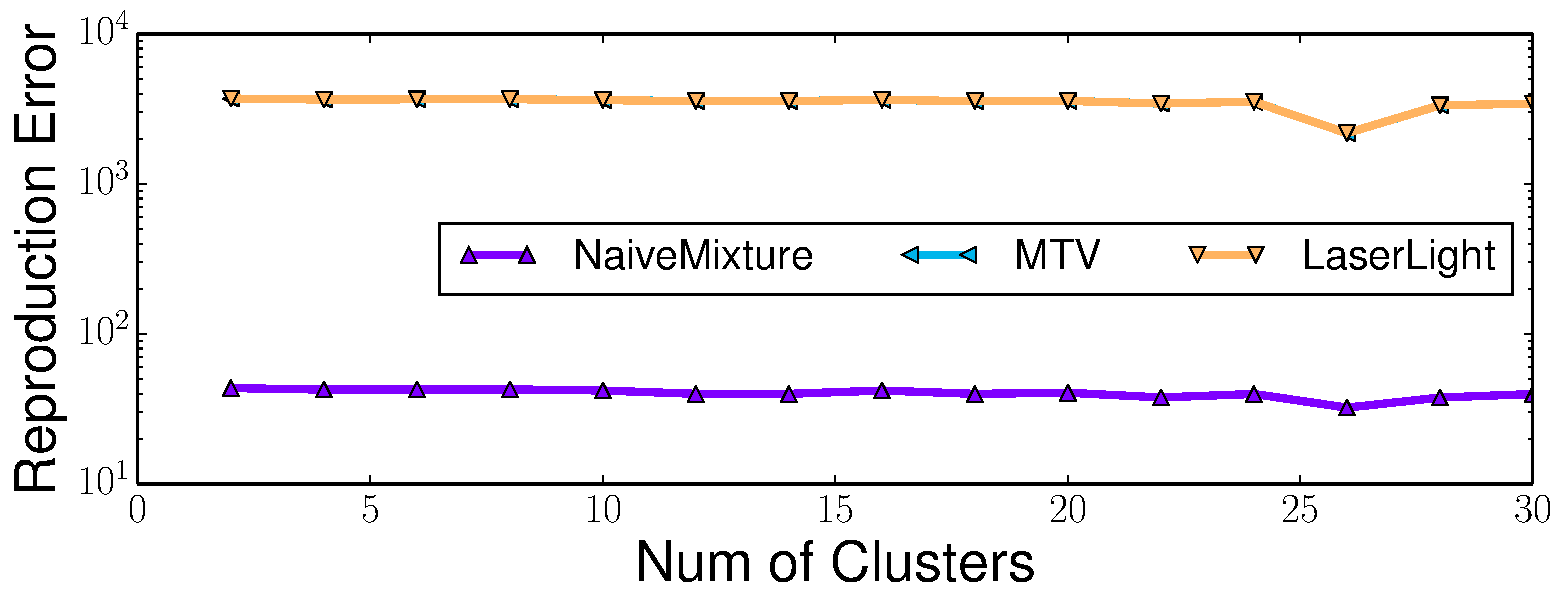
\includegraphics[width=\textwidth]{QueryLogSummarization/graphics/PatternMixtureSummaryErrorComparisonAlone_bankdata.pdf}
     \bfcaption{Naive Mixture v. LaserLight/MTV alone. Note that y-axis is in log scale.}     \label{fig:PatternMixtureEncodingErrorComparisonAlone_bankdata}
    \end{subfigure}
    ~
    \begin{subfigure}[b]{0.47\textwidth}
        \centering       
        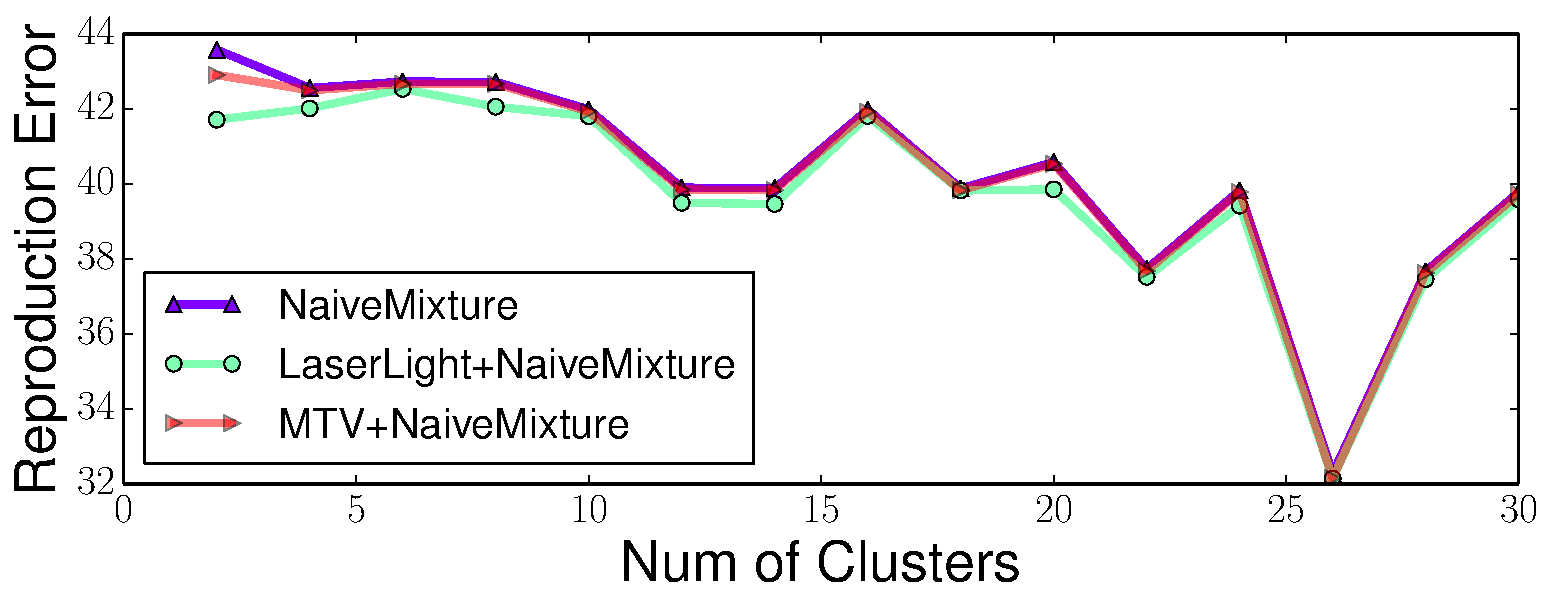
\includegraphics[width=\textwidth]{QueryLogSummarization/graphics/PatternMixtureSummaryErrorComparisonPiggybacking_bankdata.pdf}
     \bfcaption{Naive Mixture v. Naive Mixture+LaserLight/MTV. Note offset in y-axis (non-zero start).}      \label{fig:PatternMixtureEncodingErrorComparisonPiggybacking_bankdata}
    \end{subfigure}
    ~
    \begin{subfigure}[b]{0.47\textwidth}
    \centering       
    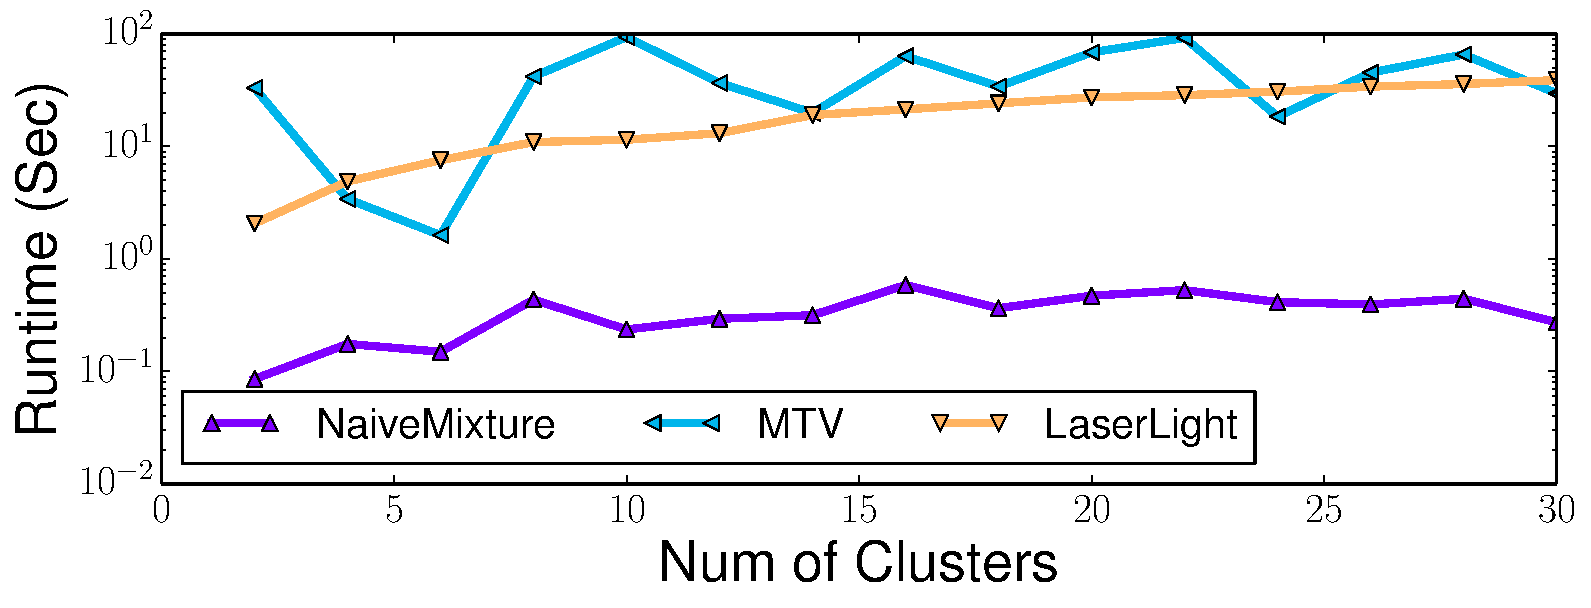
\includegraphics[width=\textwidth]{QueryLogSummarization/graphics/PatternMixtureSummaryRunningTime_bankdata.pdf}
    \bfcaption{Runtime Comparison (y-axis in log scale)}   
    \label{fig:mixtureencodingsrunningtimecomparison_bankdata}
    \end{subfigure}
\bfcaption{Feature-correlation refinement (US bank)}   \label{fig:motivatenaivemixtureencodings_bankdata}
\trimfigurewhitespace
\end{figure}

\subsubsection{Refining Naive Mixture Encodings}
\label{sec:refiningnaivemixtureencodings}
The experiment result is shown in Figure~\ref{fig:PatternMixtureEncodingErrorComparisonPiggybacking_bankdata}.
Note that I offset y-axis to show the change in Error.
We observe from the figure that reduction of Error contributed by plugging-in pattern-based summarizers is small for both algorithms.

\tinysection{Dimensionality Restriction}
For \textit{Laserlight}, the observation is partially due to the fact that I only keep top $100$ features (in terms of variability) of the data as its input, since \textit{Laserlight} is implemented in PostgresSQL 9.1 which has a threshold of $100$ arguments (one argument for each feature) that can be passed to a function.

\tinysection{Pattern Restriction}
For \textit{MTV}, this is due to a runtime error that limits us to $15$ or less patterns.
We refer the reader to Section 4.5 in~\cite{DBLP:journals/tkdd/MampaeyVT12} that explains the difficulty in inferring the maximum entropy distribution constrained by a large number of non-naive patterns.

\begin{figure}[ht!]
	\captionsetup[subfigure]{justification=centering}
    \centering
    \begin{subfigure}[b]{0.48\textwidth}
        \centering       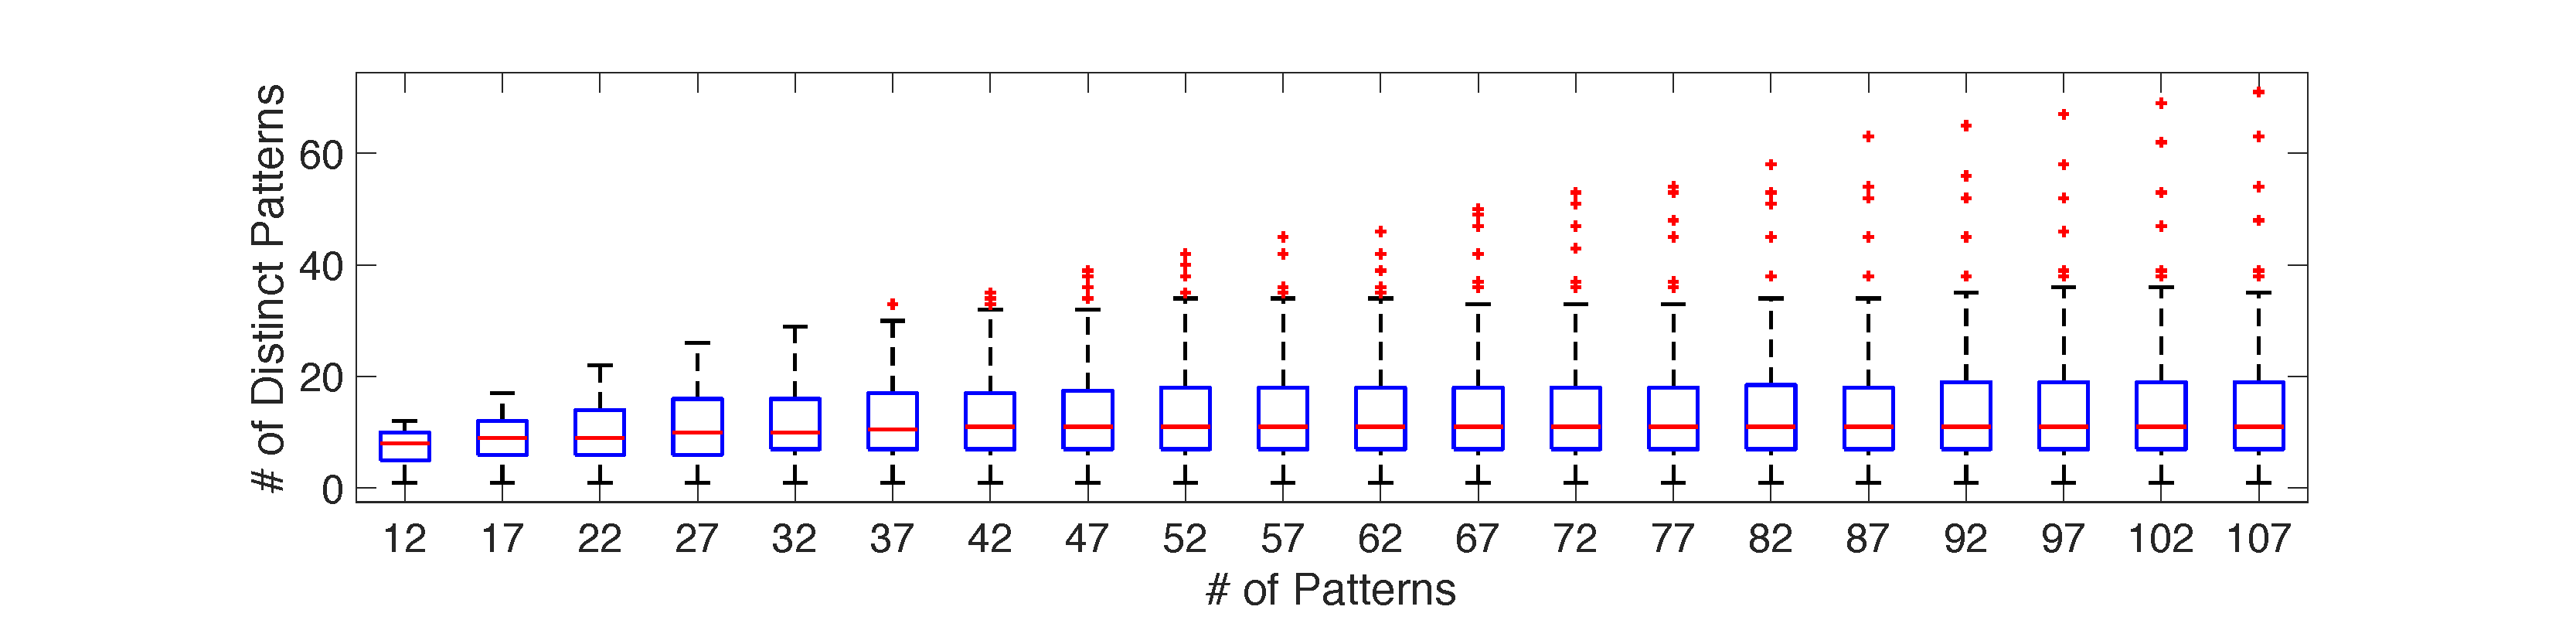
\includegraphics[width=\textwidth]{QueryLogSummarization/graphics/Laserlight_NumDistinctPatternsVNumPatterns.pdf}
 \bfcaption{Laserlight}      \label{fig:patterns_laserlight}
\end{subfigure}
    ~
\begin{subfigure}[b]{0.48\textwidth}
  \centering       
  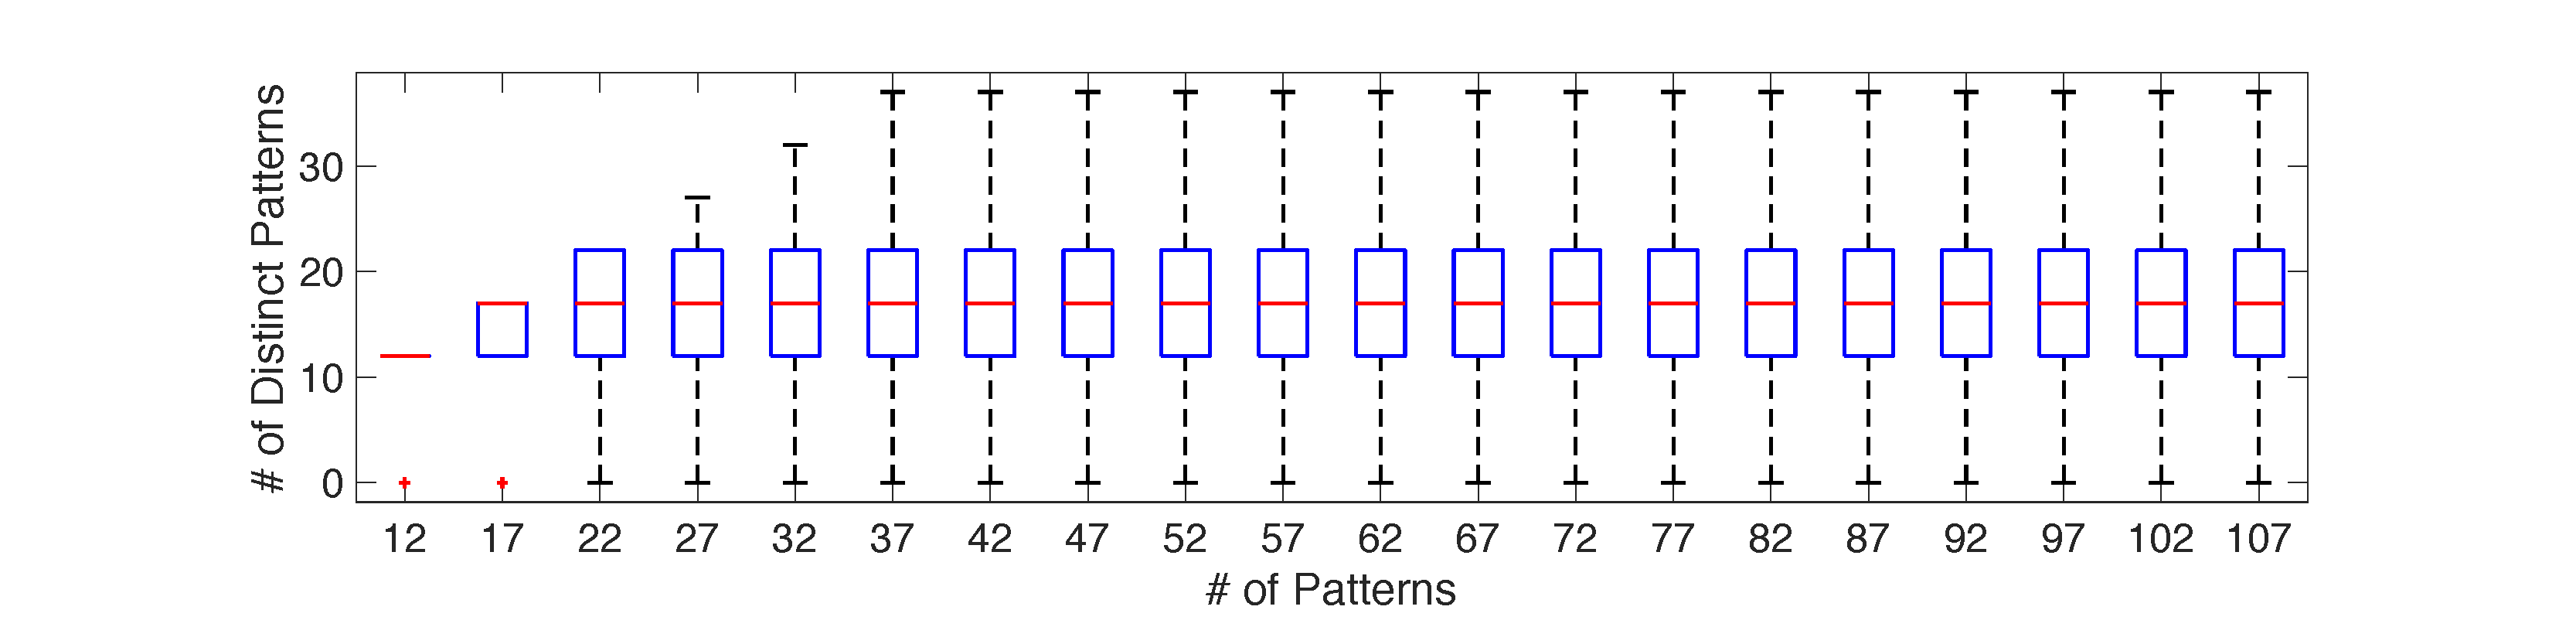
\includegraphics[width=\textwidth]{QueryLogSummarization/graphics/MTV_NumDistinctPatternsVNumPatterns.pdf}
 \bfcaption{MTV}     
 \label{fig:patterns_MTV}
\end{subfigure}
~
\bfcaption{Distinct Patterns v. Number of Patterns }   \label{fig:distinctpatternsofpatternbasedalgorithms}
\trimfigurewhitespace
\end{figure}

\tinysection{Pattern Diversification Failure}
Recall in Section~\ref{sec:naivemixtureencodingrefinement} that pattern diversification can be time-consuming.
As a result, both algorithms implement heuristics that sacrifice the capability of pattern diversification to some extent.
In other words, increase in the total number of patterns mined from \textit{Laserlight} and \textit{MTV} may not lead to commensurate increase in the number of \textit{distinct} patterns (i.e., pattern duplication implies failure in pattern diversification).
Specifically, we run \textit{MTV} and \textit{Laserlight} on each cluster ($30$ clusters in total) and vary the number of patterns configured for mining from $12$ to $107$.
We collect the number of \textit{distinct} patterns that they have mined as well as the running time under each configuration.
The experiment result is shown in Figure~\ref{fig:distinctpatternsofpatternbasedalgorithms} where y-axis is the number of distinct patterns and x-axis is the total number of patterns mined through \textit{Laserlight} and \textit{MTV}.
We observe that \textit{Laserlight} and \textit{MTV} fail to extensively explore hidden feature-correlation in our chosen datasets.

\begin{figure}[ht!]
	\captionsetup[subfigure]{justification=centering}
    \centering
    \begin{subfigure}[b]{0.48\textwidth}
        \centering       
        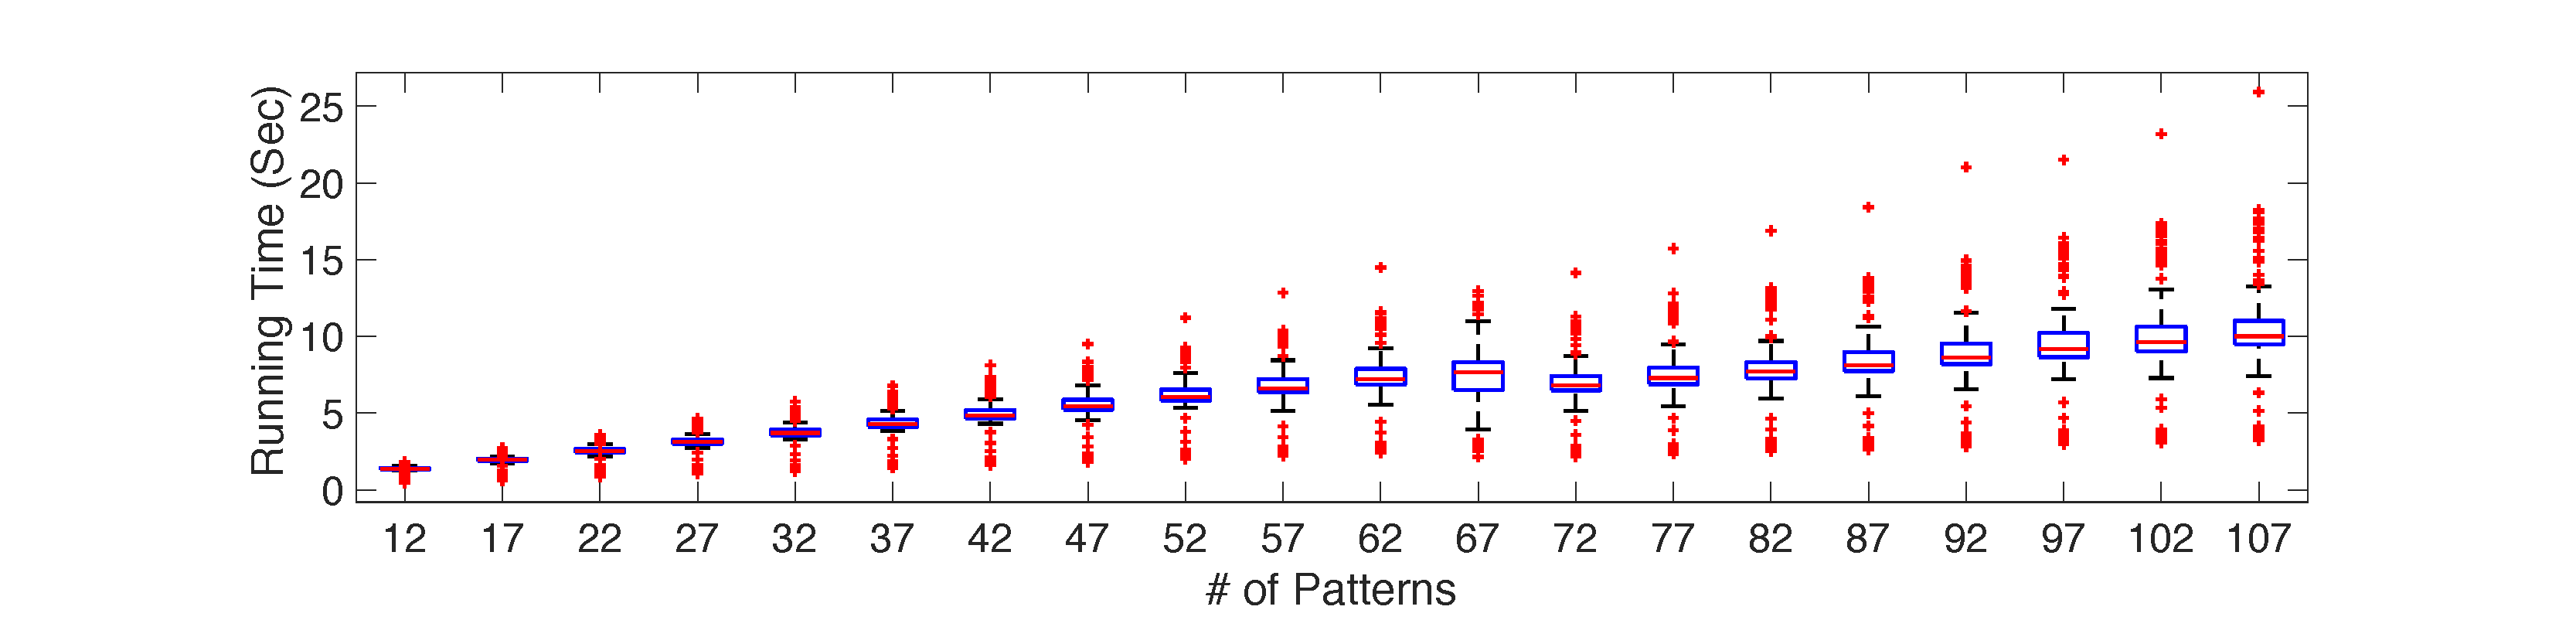
\includegraphics[width=\textwidth]{QueryLogSummarization/graphics/Laserlight_RunningTimeVNumPatterns.pdf}
 \bfcaption{Laserlight}      
 \label{fig:runningtime_laserlight}
\end{subfigure}
    ~
\begin{subfigure}[b]{0.48\textwidth}
  \centering       
  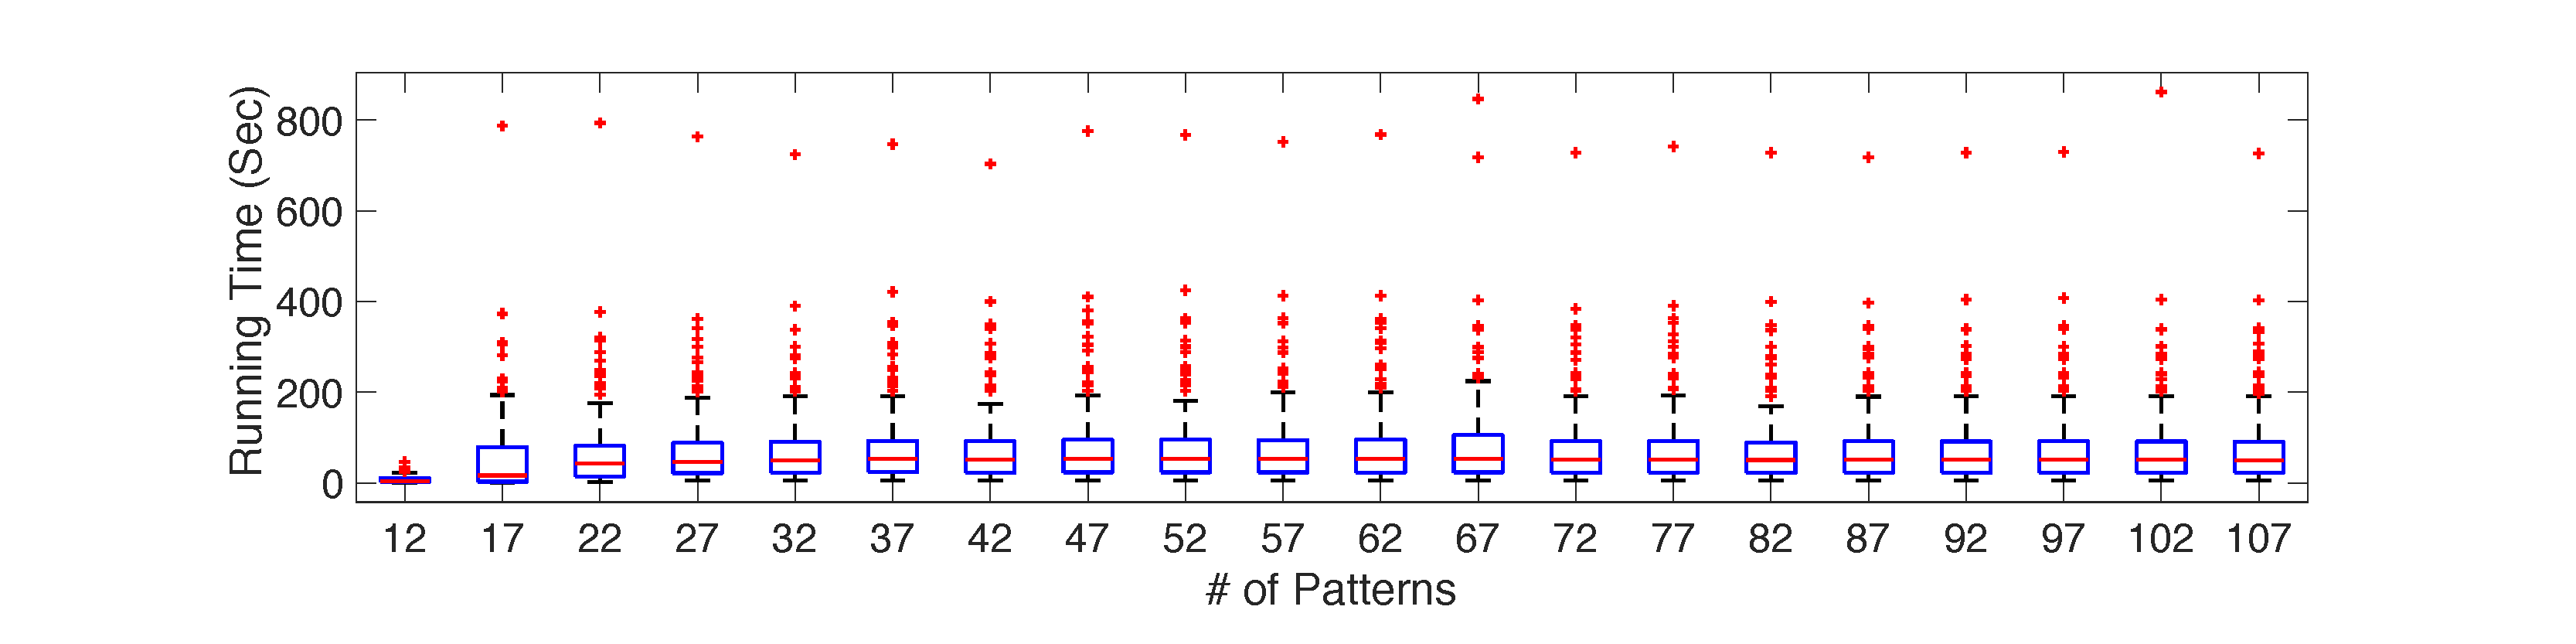
\includegraphics[width=\textwidth]{QueryLogSummarization/graphics/MTV_RunningTimeVNumPatterns.pdf}
 \bfcaption{MTV}     
 \label{fig:runningtime_MTV}
\end{subfigure}
~
\bfcaption{Running Time v. Number of Patterns}   \label{fig:runningtimeofpatternbasedalgorithms}
\trimfigurewhitespace
\end{figure}

\tinysection{Time Restriction}
Computation efficiency will also influence effectiveness of pattern based summarizers when it takes too long to mine a potentially large set of informative patterns under from the data.
The experiment result for running time analysis is shown in Figure~\ref{fig:runningtimeofpatternbasedalgorithms}.
We observe that \textit{Laserlight} shows a close-to-linear growth rate.
For \textit{MTV} the running time spikes at $17$ patterns and remains oscillating between high levels afterwards.


\section{Alternative Applications}
\label{sec:evaluatingalternativeapplications}
% !TEX root = ../paper.tex
To fairly evaluate \textit{Laserlight} and \textit{MTV}, I incorporate their own data sets and empirically evaluate them against \textit{naive mixture encoding} under their own applications.

\tinysection{Data Sets}
Specifically, I choose \textit{Mushroom} data set used in \textit{MTV}~\cite{DBLP:journals/tkdd/MampaeyVT12} which is obtained from FIMI dataset repository and U.S. Census data on Income or simply \textit{Income} data set, which is downloaded from IPUMS-USA at \textit{https://usa.ipums.org/usa/} and used in \textit{Laserlight}~\cite{DBLP:journals/pvldb/GebalyAGKS14}.
The basic statistics of the data sets are given in Table~\ref{table:extendeddatasummary}.

\begin{table}[h!]
\centering
\bfcaption{Data Sets of Alternative Applications}
\label{table:extendeddatasummary}
{\small \centering
\begin{tabular}{c c c}
\toprule
Statistics & Income & Mushroom \\
\midrule
\# Distinct data tuples & 777493 & 8124\\
\midrule
\# Features per tuple & 9 & 21\\
\midrule
Feature Binary-valued? & no& no\\
\midrule
\# Distinct features & 783 & 95\\
\midrule
Binary Classification Feature & $>100,000$? & Edibility\\
\midrule
Assumed data tuple multiplicity & 1 & 1\\
\bottomrule
\end{tabular}
}
\end{table}

\subsection{Experiments}
\label{sec:evaluatingalternativeapplicationsexperiments}
All experiments involving \textit{Laserlight} and \textit{MTV} will be evaluated under their own Error measures and data sets, unless otherwise stated.
The experiments are organized as follows: First, we establish baselines by evaluating classical \textit{Laserlight} and \textit{MTV} on their original data; Then we show that classical \textit{Laserlight} and \textit{MTV} can be generalized to partitioned data and that the generalization improves on their Error measures and also runtime; At last, we compare their generalized versions with \textit{naive mixture encoding} to show that \textit{naive mixture encoding} is a reasonable alternative.% in terms of run time and Error.

\subsubsection{Error Measures}
We first explain how \textit{naive mixture encoding} is evaluated based on Error defined by \textit{Laserlight} and \textit{MTV}.

\tinysection{Evaluating Naive Encoding on Laserlight Error}
Algorithm \textit{Laserlight} summarizes data $D$ which consists of feature vectors $t$ augmented by some binary feature $v$.
Denote the valuation of the binary feature $v$ for each feature vector $t$ as $v(t)$. 
The goal is to mine a summary encoding $\encoding$, which is a set of patterns contained in $t\in D$ that offer predictive power on $v(t)$.
Denote the estimation (based on $\encoding$) of $v(t)$ as $u_{\encoding}(t)\in [0,1]$, the \textit{Laserlight} Error is measured by $$\sum_t ( v(t)\log(\frac{v(t)}{u_{\encoding}(t)})+(1-v(t))\log(\frac{1-v(t)}{1-u_{\encoding}(t)}) )$$
Since \textit{naive encoding} $\naiveencoding$  assumes feature independence, estimation of $v(t)$ is independent of $t$, namely $u_{\naiveencoding}(t)=u_{\naiveencoding}=|\{\tau|v(\tau)=1,\tau\in D\}|/|D|$.
Consequently, the \textit{Laserlight} Error of \textit{naive encoding} is $$-|D|(u_{\naiveencoding}\log u_{\naiveencoding}+(1-u_{\naiveencoding})\log (1-u_{\naiveencoding}) )$$

\tinysection{Evaluating Naive Encoding on MTV Error}
Given binary feature vectors $D$, the \textit{MTV} Error of encoding $\encoding$ is $$-|D|H(\overline{\rho}_\encoding)+1/2|\encoding|\log|D|$$ where $H(\overline{\rho}_\encoding)$ is the entropy of maximum entropy distribution $\overline{\rho}_\encoding$ defined in Section~\ref{sec:maximumentropydistribution}.
The second term in \textit{MTV} Error penalizes Verbosity of the encoding $\encoding$.
Since naive encoding assumes feature independence, we can first compute entropy of the marginal distribution of each individual feature.
Entropy $H(\overline{\rho}_\encoding)$ is simply the sum of feature entropies.

\tinysection{Evaluating Naive Mixture Encoding}
Evaluation of \textit{naive encoding} can be generalized to \textit{naive mixture} by taking a weighted average over resulting clusters (See Section~\ref{sec:generalizedinformationlossmeasures}).

\begin{figure}[ht!]
    \captionsetup[subfigure]{justification=centering}
    \centering
    \begin{subfigure}[b]{0.48\textwidth}
        \centering       
        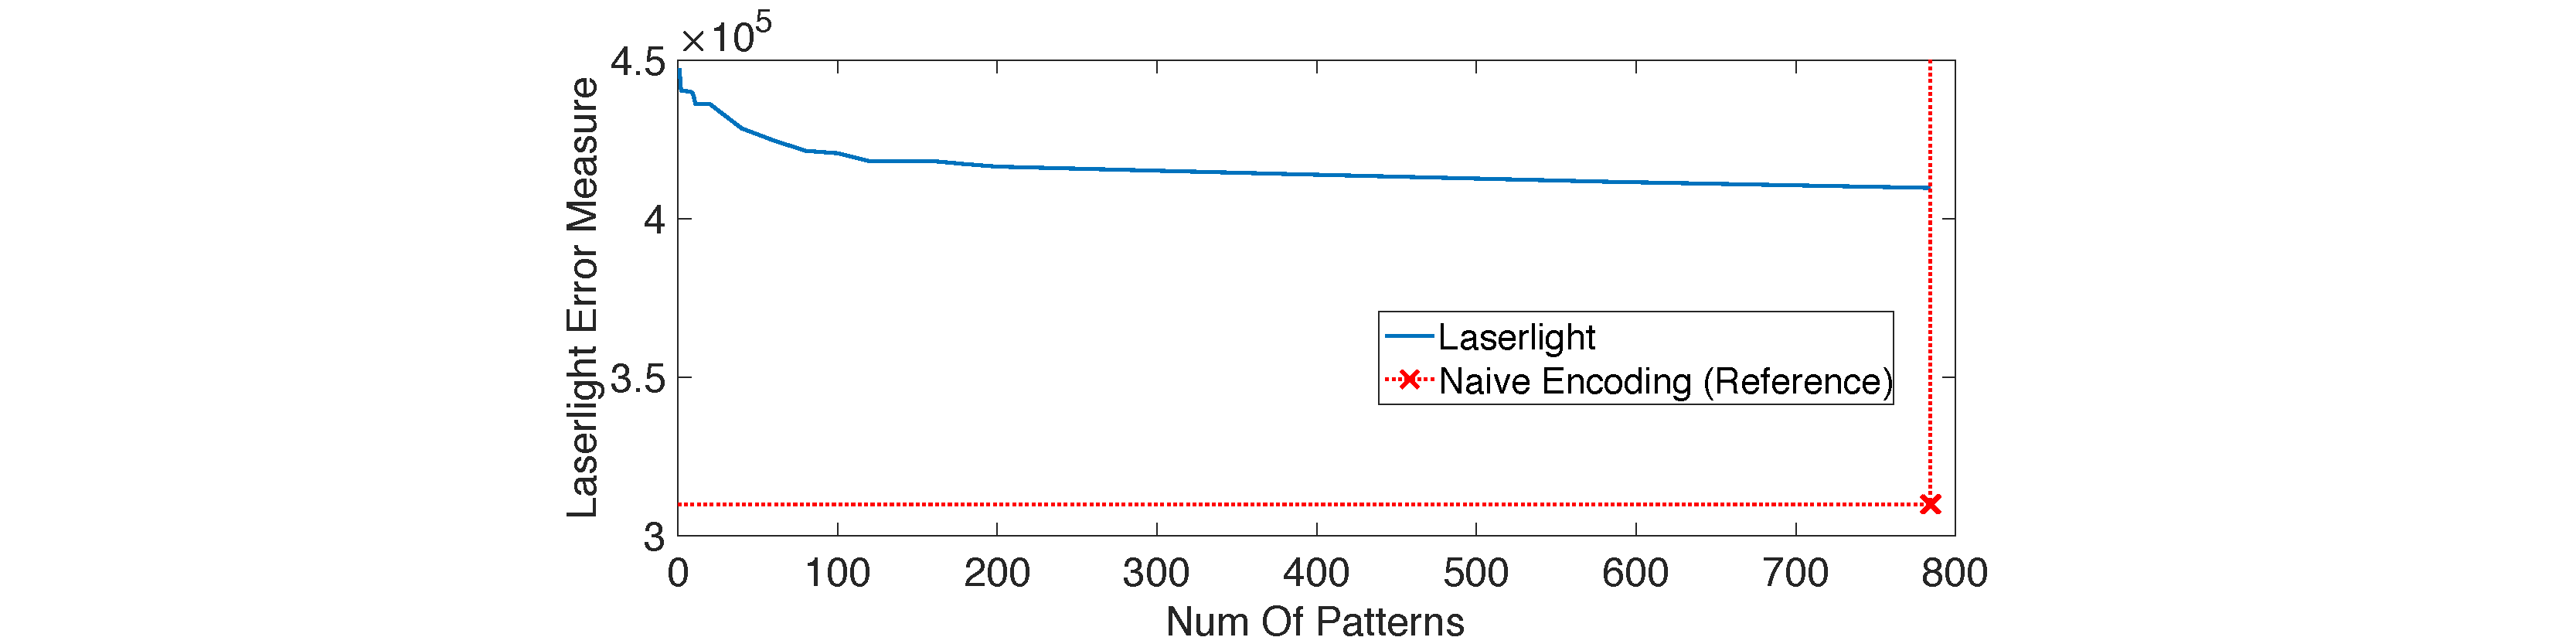
\includegraphics[width=\textwidth]{QueryLogSummarization/graphics/Laserlight_Error_vs_NumOfPatterns.pdf}
        \bfcaption{Laserlight Error v. \# of Patterns on Income data}
        \label{fig:Laserlight_Error_vs_NumOfPatterns}
    \end{subfigure}
    ~
    \begin{subfigure}[b]{0.48\textwidth}
        \centering       
        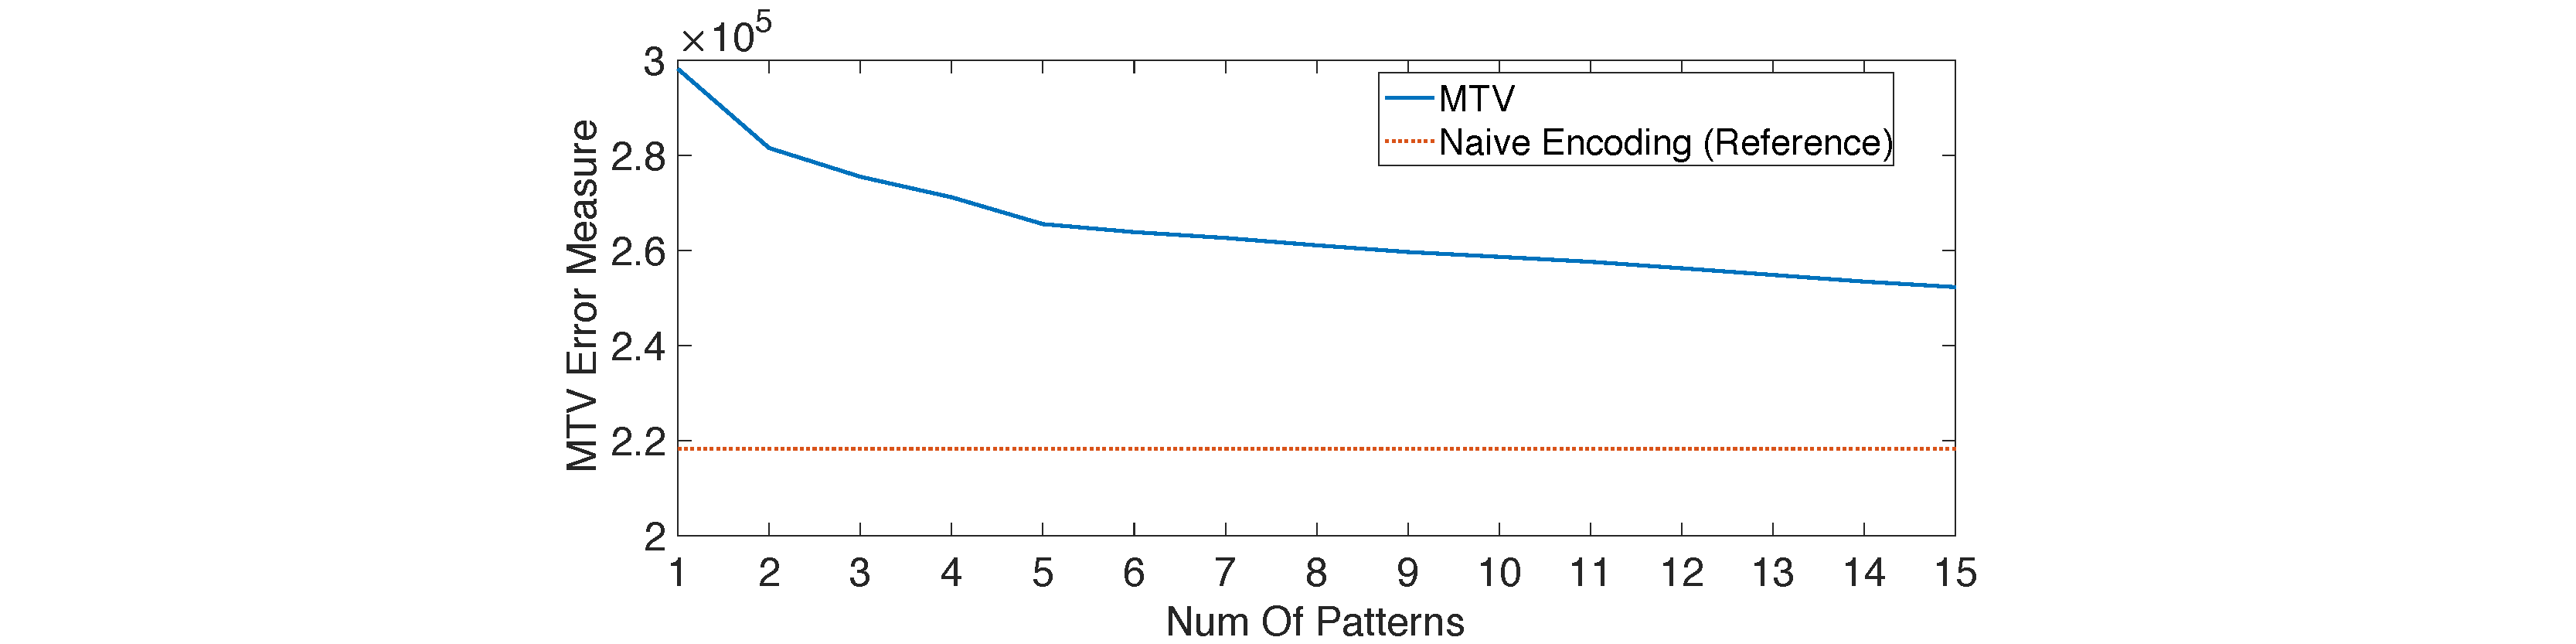
\includegraphics[width=\textwidth]{QueryLogSummarization/graphics/MTV_Error_vs_NumOfPatterns.pdf}
        \bfcaption{MTV Error v. \# of Patterns on Mushroom data}     
        \label{fig:MTV_Error_vs_NumOfPatterns}
    \end{subfigure}
    ~
    \bfcaption{Error v. Number of Patterns. Note: non-zero start of y-axis.}   
    \label{fig:performance_vs_num_of_patterns}
    \trimfigurewhitespace
\end{figure}

\subsubsection{Classical Laserlight and MTV}
\label{sec:classicallaserlightandmtv}

\tinysection{Establishing Baselines} 
To establish baselines, we evaluate \textit{Laserlight} and \textit{MTV} on their own data sets.
The take-aways from related experiments are that (1) \textit{naive encoding} is faster and more accurate than classical \textit{Laserlight} and \textit{MTV}; (2) the runtime increases superlinearly with the number of patterns mined from both \textit{Laserlight} and \textit{MTV}.

\tinysection{Dimentionality Reduction}
Recall in Section~\ref{sec:refiningnaivemixtureencodings} that \textit{Laserlight} is restricted to $100$ features.
For its own \textit{Income} data set, \textit{Laserlight} can be applied with its full set of $783$ features.
This is due to the prior knowledge that the $783$ features belong to $9$ groups.
In each group, features are mutually exclusive which can be reduced to a single feature.
Similarly, \textit{Mushroom} data set can be reduced from $95$ to $21$ features (See Table~\ref{table:extendeddatasummary}).

The results related to Error measures are given in Figure~\ref{fig:performance_vs_num_of_patterns}.
X-axis is the number of patterns and y-axis represents the Error measure of \textit{Laserlight} and \textit{MTV} in Figure~\ref{fig:Laserlight_Error_vs_NumOfPatterns} and~\ref{fig:MTV_Error_vs_NumOfPatterns} respectively.
We incorporate \textit{naive encoding} in Figure~\ref{fig:Laserlight_Error_vs_NumOfPatterns} as the reference method.
Since there are $784$ total number of features for \textit{Income} data set, the verbosity of \textit{naive encoding} will be $784$, which is shown as vertical dotted line in Figure~\ref{fig:Laserlight_Error_vs_NumOfPatterns}.
For \textit{Mushroom} data set, the verbosity of its \textit{naive encoding} will be $96$.
However, \textit{MTV} quits with error message if it is requested to mine over $15$ patterns.
Hence for Figure~\ref{fig:MTV_Error_vs_NumOfPatterns}, the limit of x-axis is $15$ and we only show Error of \textit{naive encoding} as a reference line without marking out its verbosity. 
We observe in Figure~\ref{fig:Laserlight_Error_vs_NumOfPatterns} that \textit{naive encoding} outperforms \textit{Laserlight} when their verbosity is equal (i.e., $784$).
In addition, after $100$ patterns, the slope of Error reduction becomes relatively flat.
Similar observation can be made from Figure~\ref{fig:MTV_Error_vs_NumOfPatterns}.

\begin{figure}[h!]
	\captionsetup[subfigure]{justification=centering}
    \centering

    \begin{subfigure}[b]{0.48\textwidth}
        \centering       
        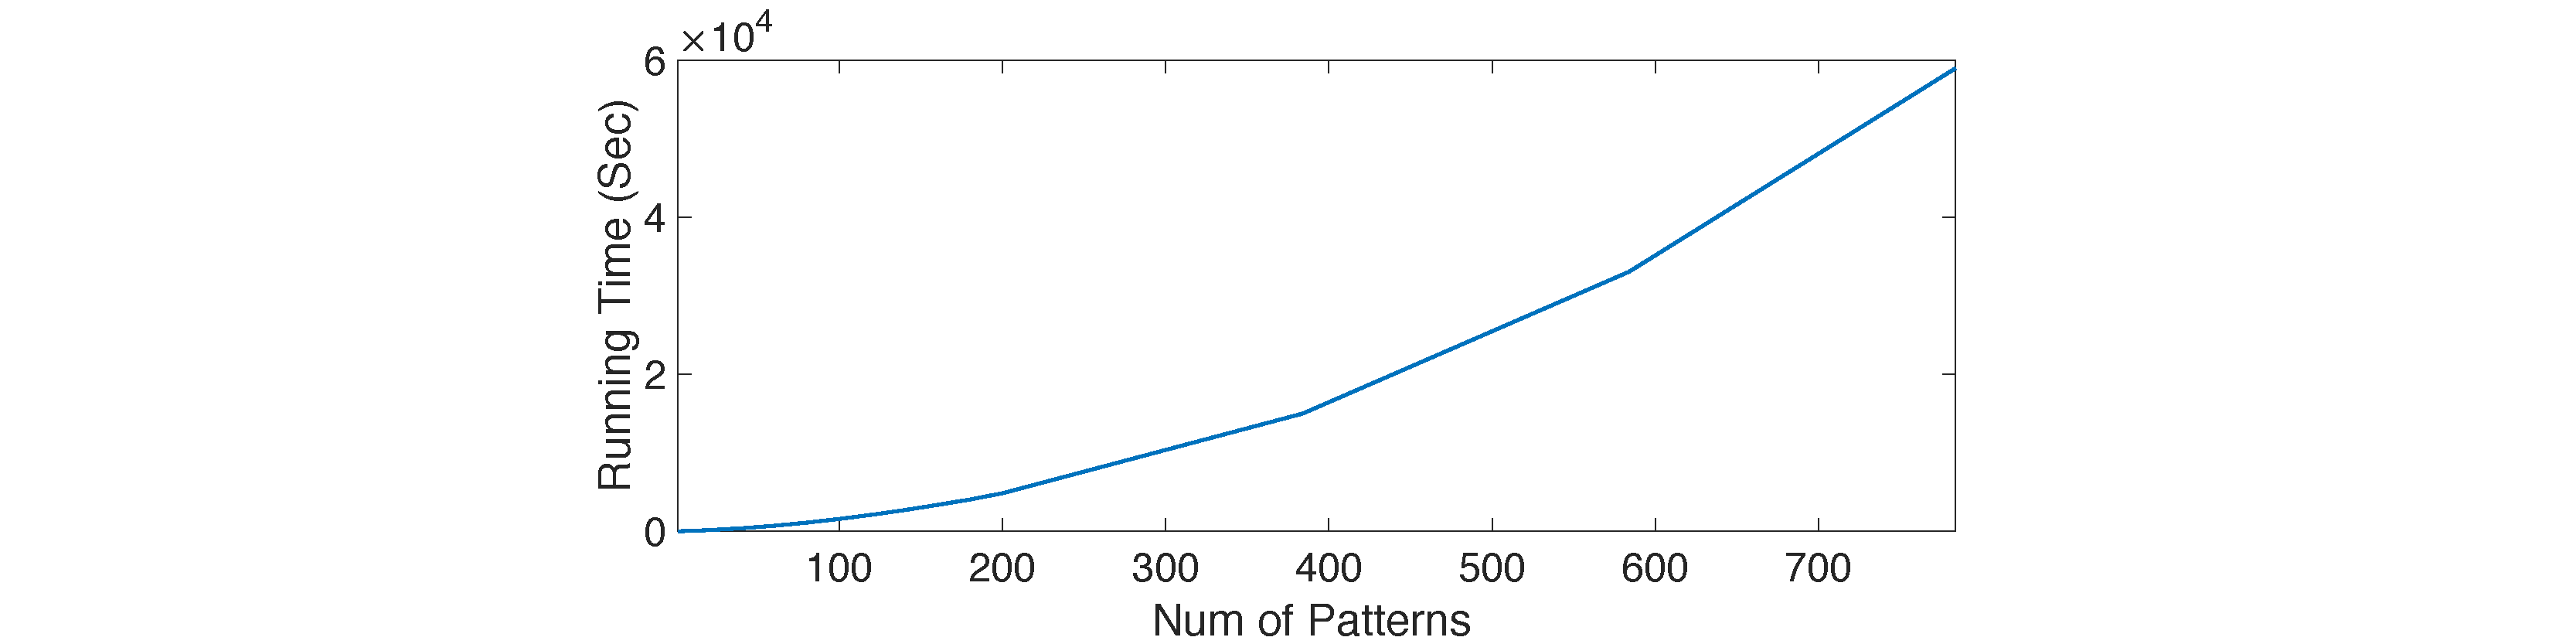
\includegraphics[width=\textwidth]{QueryLogSummarization/graphics/Laserlight_runningTimes_vs_NumOfPatterns.pdf}
 \bfcaption{Laserlight Running Time on Income Data}      \label{fig:laserlight_runningTimes_vs_NumOfPatterns}
\end{subfigure}
    ~
     \begin{subfigure}[b]{0.48\textwidth}
        \centering       
        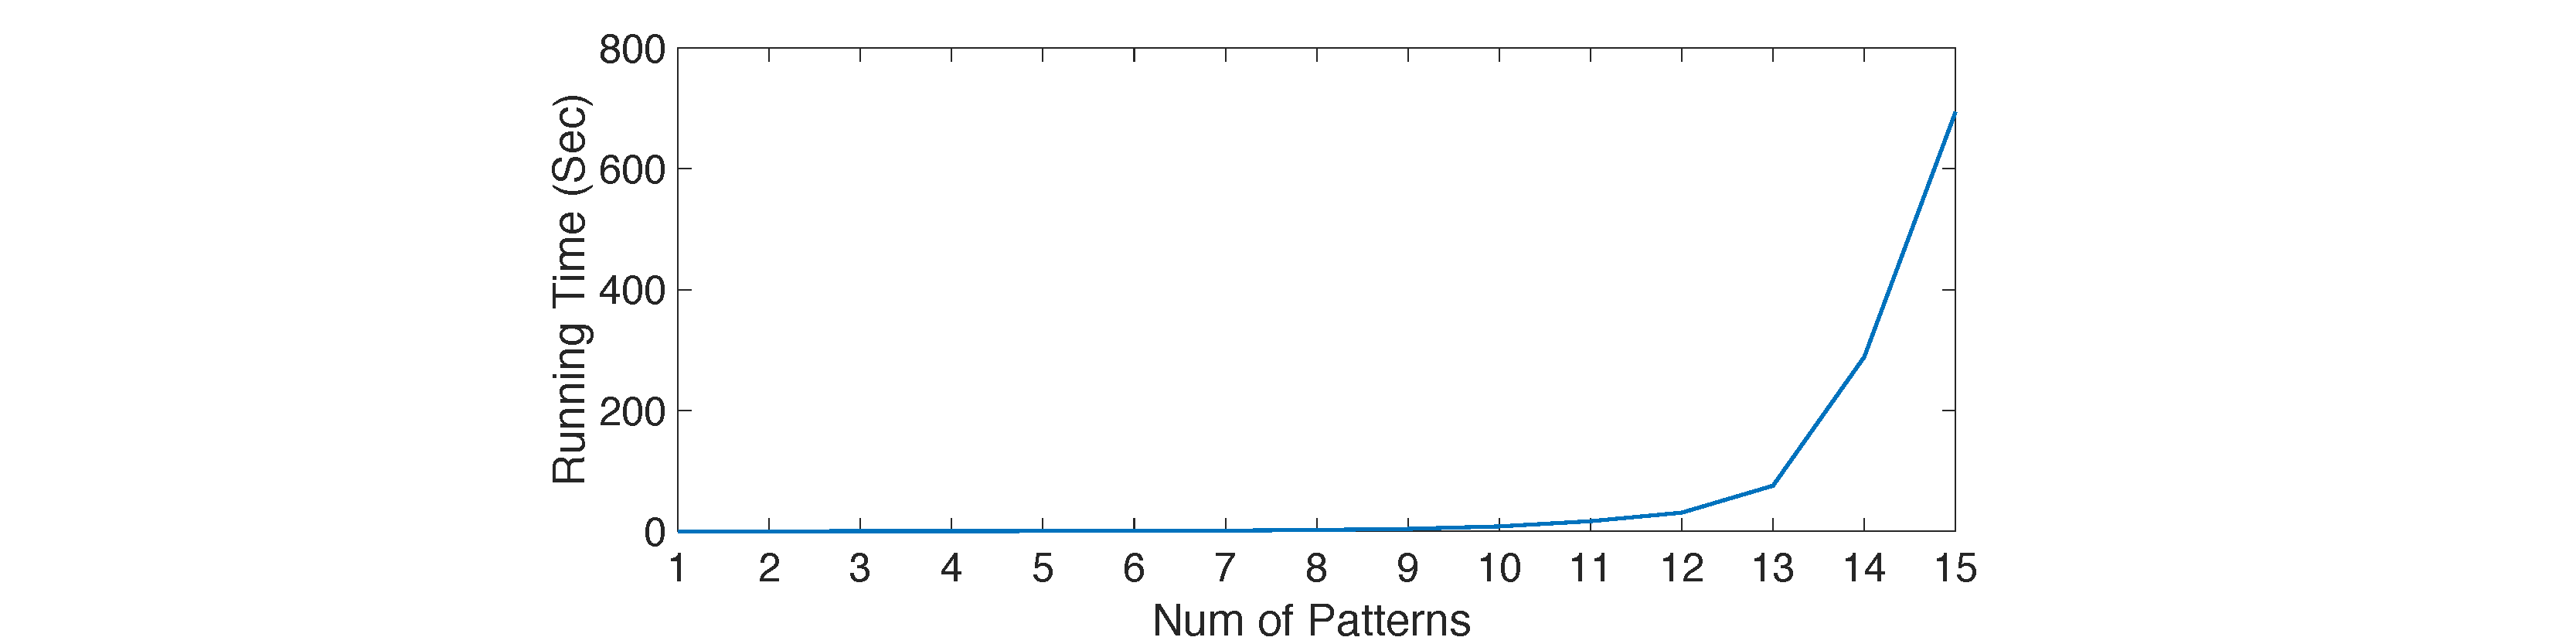
\includegraphics[width=\textwidth]{QueryLogSummarization/graphics/MTV_runningTimes_vs_NumOfPatterns.pdf}
 \bfcaption{MTV Running Time on Mushroom data}      \label{fig:mtv_runningTimes_vs_NumOfPatterns}
\end{subfigure}
    ~   
\bfcaption{Running Time of Laserlight and MTV}   \label{fig:runningTime_analysis}
\trimfigurewhitespace
\end{figure}

Next I show corresponding run time results in Figure~\ref{fig:runningTime_analysis}.
We observe that the running time increases exponentially with the number of patterns, for both \textit{Laserlight} and \textit{MTV}.

\subsubsection{Generalizing Laserlight and MTV}
\label{sec:generalizinglaserlightandmtv}
In this section, we generalize \textit{Laserlight} and \textit{MTV} on partitioned data by applying them on each cluster.
We then combine Errors on all clusters by taking a weighted average, as described in Section~\ref{sec:generalizedinformationlossmeasures}.
Depending on how many patterns are mined from each cluster, \textit{Laserlight} and \textit{MTV} can be generalized into two types: (1) The number of patterns mined from each cluster is scaled to be equal to Verbosity of the \emph{naive encoding}; and (2) The total number of patterns mined from all clusters is fixed to a given number.
I name the first type \emph{Laserlight (MTV) Mixture Scaled}, which is comparable to \emph{naive mixture encoding}.
I name the second type \emph{Laserlight (MTV) Mixture Fixed}, which is comparable to the classical \emph{LaserLight (MTV)} algorithm.

\tinysection{Take-away}
As the data is partitioned into more clusters, both runtime and Error of \emph{Laserlight (MTV) Mixture Fixed} exponentially decrease.
This observation can be potentially generalized to other pattern mining algorithms.
For experiment details, I refer the reader to~\cite{DBLP:journals/corr/abs-1809-00405}.

\begin{figure}[h!]
	\captionsetup[subfigure]{justification=centering}
    \centering
    \begin{subfigure}[b]{0.47\textwidth}
        \centering       
        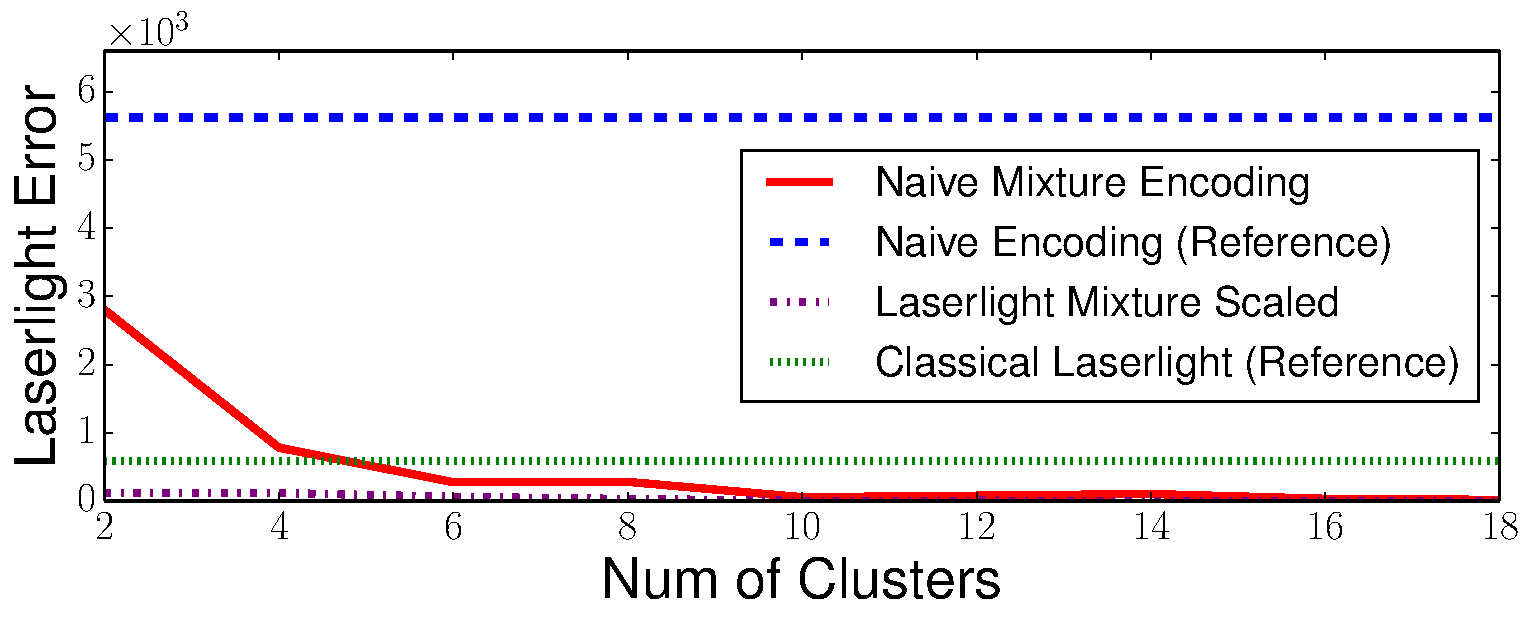
\includegraphics[width=\textwidth]{QueryLogSummarization/graphics/Laserlight_Errors_vs_NumOfClusters.pdf}
 \bfcaption{Laserlight Error v. \# of Clusters on Mushroom data}      \label{fig:LaserlightMixture_Errors_vs_NumOfClusters}
\end{subfigure}
    ~
\begin{subfigure}[b]{0.47\textwidth}
  \centering       
  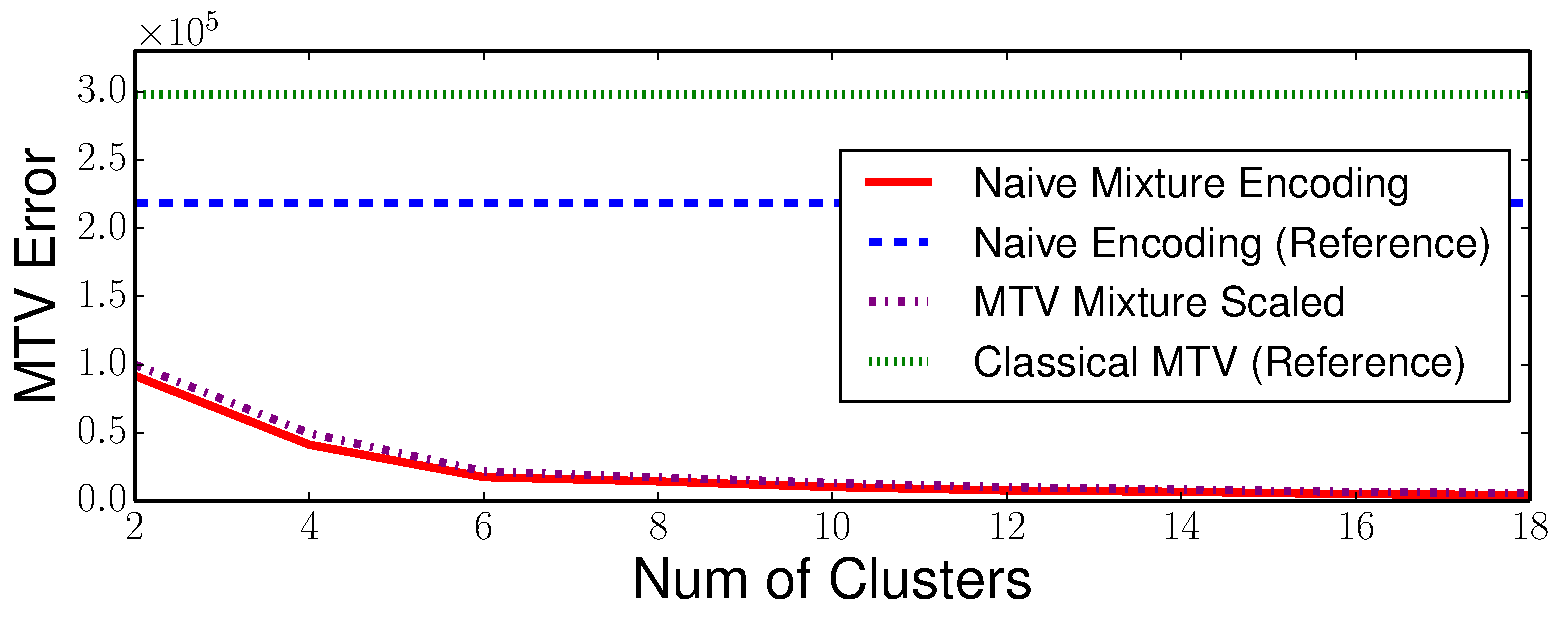
\includegraphics[width=\textwidth]{QueryLogSummarization/graphics/MTV_Error_vs_NumOfClusters.pdf}
 \bfcaption{MTV Error v. \# of Clusters on Mushroom data}     
 \label{fig:MTVMixture_vs_Laserlight_runningTimes_IncomeData}
\end{subfigure}
~
\bfcaption{Naive Mixture v. Laserlight/MTV Mixture}   
\label{fig:Naive Mixture Encoding_vs_Laserlight&MTV_Mixture}
\trimfigurewhitespace
\end{figure}
\subsubsection{Comparison with Naive Mixture Encoding}
\label{sec:Evaluating_Naive_Mixture_Encoding}

At last, we compare \emph{Laserlight (MTV) Mixture Scaled} with \emph{naive mixture encoding}.
Note that it is time-consuming for \emph{Laserlight} to mine the same number of patterns as \emph{naive encoding} on \emph{Income} data (See runtime analysis in~\cite{DBLP:journals/corr/abs-1809-00405}), I choose \emph{Mushroom} data for \emph{Laserlight Mixture Scaled} instead.
The experiment results are given in Figure~\ref{fig:Naive Mixture Encoding_vs_Laserlight&MTV_Mixture}. 
The x-axis for all sub-figures in Figure~\ref{fig:Naive Mixture Encoding_vs_Laserlight&MTV_Mixture} represents the number of clusters and the y-axes stands for \emph{Laserlight} and \emph{MTV} Error respectively.
I incorporate baselines (i.e., \emph{naive encoding}, classical \emph{Laserlight} and \emph{MTV}) as reference lines in Figure~\ref{fig:LaserlightMixture_Errors_vs_NumOfClusters} and~\ref{fig:MTVMixture_vs_Laserlight_runningTimes_IncomeData} respectively.
We also experienced a limitation of $15$ patterns for \emph{MTV}.
Hence the comparison between \emph{MTV Mixture Scaled} and {naive mixture encoding} is not strictly on equal footing as \emph{MTV Mixture Scaled} is not able to reach the same Total Verbosity as \emph{naive mixture encoding}.
Note that their difference in Verbosity is mitigated by the fact that \emph{MTV} Error measure penalizes encoding Verbosity.

Figure~\ref{fig:LaserlightMixture_Errors_vs_NumOfClusters} shows that both \emph{naive mixture encoding} and \emph{Laserlight Mixture Scaled} have lower Error than their baselines.
In addition, \emph{Laserlight Mixture Scaled} has lower Error than \emph{naive mixture encoding} when the number of clusters is less than $4$ and they become close after $6$ clusters.
In other words, \emph{Laserlight} is more accurate on lightly partitioned data. 
As the data is further partitioned, clusters become easier to summarize, and \emph{naive encoding} becomes more similar to \emph{Laserlight}.
Figure~\ref{fig:MTVMixture_vs_Laserlight_runningTimes_IncomeData} shows that \emph{naive mixture encoding} marginally outperforms \emph{MTV Mixture Scaled}.

\tinysection{Take-away}
\emph{Naive mixture encoding} is faster and has similar (lower) Error than \emph{Laserlight (MTV) Mixture Scaled}.


\section{Related Work}
\label{sec:backgroundandrelatedwork}
% !TEX root = ../paper.tex
%The focus of this paper is to model user intents via query monitoring. Provided that an accurate model can be created, it would lead not only to effective insider attack detection systems, but could have implications for other fields like database performance optimizers.

%There are some upfront security policies used and enforced in organizations to protect the integrity and confidentiality of the resources.
%For instance, as a multi-level security (MLS) policy, \textit{Bell-LaPadula}~\cite{bellLaPadula} has very rigid constraints, and does not tolerate normal changes in business needs over time. Policies like the \textit{Chinese Wall Security Model}~\cite{ChineseWall} focus on preventing conflicts of interest in a commercial domain rather than explicitly protecting resources. A more permissive approach is based on role-based access control (RBAC)~\cite{rolebased}, where predetermined user groups are permitted to perform specific tasks.  However, even here, the specific tasks performed by each group might evolve over time.%There are also security policies especially tailored for preventing insider attacks~\cite{pramanik2004security} and enforcing policies~\cite{enforceable2000}. 
%Although useful, these policies cannot prevent insider attacks as there are often policy violations and exceptions in the implementation~\cite{bishop2010risk}. These exceptions can be explained with the \textit{Oracle Policy}, \textit{Feasible Policy} and \textit{Configuration Policy} concepts~\cite{bishop2010risk}. \textit{Oracle Policy} represents the ideal case which is what the policy maker actually intends with the policy. It can be non-deterministic but it supplies a correct answer for any question asked as it covers the intent and custom. \textit{Feasible Policy} substitutes the ideal case with an implementation of it on a computer system. Lastly, \textit{Configuration Policy} expresses the application of the \textit{Feasible Policy} on a particular system. This means that the ideal case expressed in the policy may not always be enforced on the computer system.

%The basic idea behind \sysname{} is to profile normal user behavior, detect suspicious behavior using this information, and distinguish malicious behavior from benign intents~\cite{Kul2015Jowua}. 
%Indeed, this idea is not new; there are many anomaly detection systems focusing on suspicious behavior of users.  
%Specific examples include file access~\cite{wang2016fileaccess} and transfers~\cite{Arief2015Jowua}, online and social behavior~\cite{Gavai2015Jowua}, activities on a website~\cite{manavoglu2003network}, command-line statements~\cite{maxion2002masquerade} and SQL queries issued to a database~\cite{Mathew2010Raid}. 

%\textbf{SQL queries as a resource:}
%As the basic unit of interaction between a database and its users, the sequence of SQL queries that a user issues effectively models the user's behavior. Also, queries that are similar in nature imply that they might be issued to perform similar duties. Hence, auditing SQL query logs of the databases and having a sense of what the query intends to do correctly gains a lot of importance.

%\textit{Query interpretation} is the problem of understanding the goal of the query and it is regarded as hard as writing a new query as the complexity of the query increases~\cite{gatterbauer2011databases}. QueryViz~\cite{Danaparamita2011queryviz} addresses this problem by visualizing the query. It takes SQL query and the schema of the database; and parses the query, builds an AST and creates a graph for users to view it. The aim is to present queries as simple as possible for the users to understand them, as it is easier to understand the relationships and references in a query when it is graphically visualized.

%However, it is more practical to analyze large SQL query logs as a whole. Generating query cluster visualizations is still a complex task considering that even visualizing just one query accurately to help users understand the intent behind the query quickly is still a research challenge~\cite{gatterbauer2011databases}. 

%The authors of~\cite{Kamra2007SyntaxBased} focus on detection of potential intrusions on database systems. In their paper, they introduce a mechanism which analyzes audit logs of databases with both defined user roles and undefined user roles. This system uses multiple techniques to attempt to detect the threats depending on the role distinction and builds user profiles.
%For representing their data, the authors use a quiplet relation. This relation contains data bases on the command, the projection data, and the selection data. To further expand on this data representation, the authors use fine, medium, and coarse-quiplets, with less data represented in the respective relations. In a Role Based Access Control (RBAC) system, the authors use Naive Bayes Classifier to test profiles built from the quiplet information. In their testing using synthesized data against the profiles, the fine-quiplets performed best of the relations in both false positives and false negatives.
%They use Naive Bayes Classifier and clustering techniques, k-centers and k-means, in their experiments to build user profiles.
%The techniques were able to produce low false positives in experimental testing, but the false negative rates were high for both techniques.
%Their work shows that building user profiles from database logs has potential for detecting intrusions, especially in a system with defined roles.

We aim at compressing query logs for accurately and efficiently computing workload statistics.
Before the discussion of compression, we first review usecases and related work for workload analysis.

\subsection{Workload Analysis}
Existing approaches related to workload analysis usually aim at specific tasks like query recommendation~\cite{DBLP:conf/icdm/MittalVCEP10,DBLP:journals/jdwm/GiacomettiMNS11,DBLP:journals/pvldb/KhoussainovaKBS11,DBLP:conf/icde/YangPS09,DBLP:journals/kais/AligonGMRT14}, performance optimization~\cite{DBLP:conf/adbis/AouicheJD06,DBLP:conf/sigmod/BrunoCG01}, outlier detection~\cite{DBLP:journals/vldb/KamraTB08} or visual analysis~\cite{DBLP:conf/simbig/MakiyamaRS15}. 

\tinysection{Query Recommendation}
This task aims at tracking historical querying behavior and generating query recommendations.
Related approaches~\cite{DBLP:conf/icdm/MittalVCEP10,DBLP:journals/pvldb/KhoussainovaKBS11} flatten a query \textit{abstract syntax tree} as a set of \textit{fragments}~\cite{DBLP:conf/icdm/MittalVCEP10} or \textit{snippets}~\cite{DBLP:journals/pvldb/KhoussainovaKBS11}.
User profiles are then built by grouping and summarizing queries of specific users in order to make personalized recommendation. 
Under OLAP systems, profiles are also built for workloads of similar OLAP sessions~\cite{DBLP:journals/kais/AligonGMRT14}.

\tinysection{Performance Optimization}
Index selection~\cite{DBLP:conf/vldb/ChaudhuriN97,DBLP:journals/tods/FinkelsteinST88} and materialized view selection~\cite{DBLP:conf/vldb/AgrawalCN00,DBLP:conf/adbis/AouicheJD06,DBLP:conf/sigmod/BrunoCG01} are typical performance optimization tasks.
The configuration search space is usually large, but can be reduced with appropriate summaries.

\tinysection{Outlier Detection}
Kamra \textit{et al.}~\cite{DBLP:journals/vldb/KamraTB08} aim at detecting anomalous behavior of queries in the log by summarizing query logs into profiles
of normal user behavior.

\tinysection{Visual Analysis}
Makiyama \textit{et al.}~\cite{DBLP:conf/simbig/MakiyamaRS15} provide a set of visualizations that facilitate further workload analysis on Sloan Digital Sky Survey (SDSS) dataset.
QueryScope~\cite{DBLP:journals/pvldb/HuRCLZ08} aims at finding better tuning opportunities by helping human experts to identify patterns shared among queries. 
%

In these approaches, queries are commonly encoded as feature vectors or bit-maps where a bit array is mapped to a list of features with $1$ in a position if the corresponding feature appears in the query and $0$ otherwise.
Workloads under the bit-map encoding must then be compressed before they can be efficiently queried or visualized for analysis. 
\subsection{Workload Compression Schemes}
\tinysection{Run-length Encoding}
\textit{Run-length encoding (RLE)} is a loss-less compression scheme commonly used in \textit{Inverted Index Compression}~\cite{DBLP:books/nostrand/WittenMT94,DBLP:journals/csur/ZobelM06} and \textit{Column-Oriented Compression}~\cite{DBLP:conf/sigmod/AbadiMF06}.
RLE-based compression algorithms include but not limited to: Byte-aligned Bitmap Code (BBC) used in Oracle systems~\cite{DBLP:journals/vldb/AntoshenkovZ96}, Word-aligned Hybrid (WAH)~\cite{DBLP:conf/ssdbm/WuOS02} and many others~\cite{DBLP:journals/acj/MoffatZ94,DBLP:conf/vldb/JohnsonA00,Antoshenkov:1995:BBC:874051.874730}.
In general, RLE-based methods focus on column-wise compression and requires additional heavyweight inference on frequencies of cross-column (i.e., row-wise) patterns used for workload analysis.

\tinysection{Lempel-Ziv Encoding}
Lempel-Ziv~\cite{DBLP:journals/tit/ZivL77,DBLP:journals/tit/ZivL78} is the loss-less compression algorithm used by gzip.
It takes variable sized patterns (row-wise in our case) and replaces them with fixed length codes, in contrast to Huffman encoding~\cite{4051119}. 
Lempel-Ziv encoding does not require knowledge about pattern frequencies in advance and builds the pattern dictionary dynamically. 
There are many other similar schemes for compressing files represented as sequential bit-maps, e.g.~\cite{DBLP:conf/adbis/SkibinskiS07a}.

\tinysection{Dictionary Encoding}
\textit{Dictionary encoding} is a more general form of Lempel-Ziv.
It has the advantage that patterns with frequencies stored in the dictionary can be interpreted as workloads statistics useful for analysis.
%Practically it is not feasible to enumerate all patterns in a dictionary and only a subset of \textit{frequent patterns}~\cite{Han:2007:FPM:1275092.1275097} may be selected.
In this paper, we extend dictionary encoding and focus on using a dictionary to infer frequencies of patterns not in it.
%Hence it is critical to have a quality measure that is efficiently computatble and reflects the overall deviation on inferring workload statistics using existing patterns in the dictionary.
Mampaey \textit{et al.} proposed \textit{MTV} algorithm~\cite{DBLP:journals/tkdd/MampaeyVT12} that finds the dictionary (of given size) having optimal \textit{Bayesian Information Criterion(BIC)} score.
Gebaly \textit{et al.} proposed \textit{Laserlight} algorithm~\cite{DBLP:journals/pvldb/GebalyAGKS14} that builds a pattern dictionary for correctly inferring the truth-value of some augmented binary feature.

\tinysection{Generative Models}
A generative model is a lossy compressed representation of the original log.
Typical generative models are \textit{probabilistic topic models}~\cite{DBLP:journals/cacm/Blei12,DBLP:conf/acl/WangZLG09} and \textit{noisy-channel} model~\cite{DBLP:journals/ai/KnightM02}.
Generative models can infer pattern frequencies but they lack a model-independent measure for efficiently evaluating overall inference accuracy.

\tinysection{Matrix Decomposition}
Matrix decomposition methods including Principal Component Analysis (PCA)~\cite{DBLP:reference/stat/Jolliffe11} and Non-negative matrix factorization (NMF)~\cite{lee1999learning} offer lossy data compression.
But the resulting matrices after decomposition are not suited for inferring workload statistics.

%An extensively studied problem \textit{Text Summarization} is closely-related. 
%Its objective is condensing the source text, which is a collection/sequence of sentences into a shorter version preserving its information content and overall meaning. 
%Methods achieving such objective can be classified into two categories~\cite{article}: (1) abstractive and (2) extractive.
%
%An extractive summarization is simply ranking and extracting \textit{representative} or \textit{relevant} records from the source log.
%Different extractive methods only differ in the measure of relevance.
%The simplest measure would be \textit{Term frequency-inverse document frequency (TF-IDF)}~\cite{4782490}. More sophisticated measures include but not limited to \textit{Lexical Chain} based~\cite{Barzilay97usinglexical}, \textit{graph-based  lexical centrality}~\cite{Erkan:2004:LGL:1622487.1622501}, \textit{latent semantic analysis} based~\cite{Gong:2001:GTS:383952.383955}, \textit{machine learning} based~\cite{Neto:2002:ATS:645853.669480}, \textit{hidden markov model} based~\cite{Conroy:2001:TSV:383952.384042}, \textit{neural network} based~\cite{1344634}, \textit{query} based~\cite{Pembe2010AutomatedQA}, \textit{mathematical regression} based~\cite{fattah2008automatic} and \textit{fuzzy-logic} based~\cite{4529844}.
%
%A survey on extractive methods~\cite{article} pointed out two of their problems: (1) Not all text in extracted records are relevant, resulting in unnecessary verbosity and (2) Relevant information tends to either overlap or spread among records, resulting in unexpectedly large amount of records extracted to achieve reasonable coverage on information content.
%These problems can be solved by extracting only \textit{patterns} or fragments commonly shared by records, e.g \textit{frequent pattern mining}~\cite{Han:2007:FPM:1275092.1275097}.
%Frequency is not the only measure of relevance for patterns.
%Mampaey \textit{et al.}~\cite{DBLP:journals/tkdd/MampaeyVT12} study the problem of summarizing multi-dimensional vectors where all attributes are binary. 
%The summary is represented as a set of \textit{most informative} patterns which maximize the \textit{Bayesian Information Criterion} (BIC) score.
%Gebaly \textit{et al.}~\cite{DBLP:journals/pvldb/GebalyAGKS14} aim at summarizing multi-dimensional categorical-valued vectors augmented by a binary attribute. 
%The relevance of pattern depends on whether it can \textit{explains} the valuation of the augmented attribute.
%
%However, there is still controversy on summary evaluation for extractive methods.
%Evaluation measures such as ROGUE~\cite{Lin04rouge:a} and BLEU~\cite{Papineni:2002:BMA:1073083.1073135} are human-involved.
%Since human can only participate as reference summarizers in data sets limited in size and number, it is controversial that the performance of a summarizer evaluated on existing limited data sets will generalize to unseen real life data sets.
%
%An abstractive summarization attempts to go beyond extraction and builds up probabilistic generative models.
%The goal is to search for relevant \textit{topics}~\cite{DBLP:journals/cacm/Blei12} or \textit{abstracts}~\cite{DBLP:journals/ai/KnightM02} represented by latent variables in the model inferred from the data in the log.
%A probabilistic model is usually called generative as it is able produce a world of possible logs where the log representing the actual data has the maximum likelihood to be produced (i.e. Maximum Likelihood Estimate).
%Typical models used for summarization are \textit{probabilistic topic models}~\cite{DBLP:journals/cacm/Blei12,DBLP:conf/acl/WangZLG09} and \textit{noisy-channel} model~\cite{DBLP:journals/ai/KnightM02}.
%
%Abstractive summarization using probabilistic models has its own problems.
%Firstly, goodness of fit on data (i.e., likelihood) is model-dependent and cannot be used to compare different models.
%As a result, the general practice of evaluating probabilistic models is also using human as reference summarizers (see~\cite{DBLP:journals/ai/KnightM02,DBLP:conf/acl/WangZLG09}).
%Hence similar controversy in summary evaluation still exists.
%In addition, as~\cite{article} pointed out, the world of logs that any model can produce (i.e., model capacity) is limited.
%There may exist logs that exceeds model capacity.
%Finally, unlike understanding extracted records or shared patterns, it may require a steep learning curve for an human observer to consume and utilize information conveyed by probabilistic models.



% Existing approaches for log summarization are frequently aimed at specific tasks like query recommendation~\cite{chatzopoulou2011querie, giacometti2009,magda2010snipsuggest,yang2009}, performance optimization~\cite{aouiche2006,Bruno:2001:SMW:375663.375686},  session identification~\cite{Aligon2014}, outlier detection~\cite{Kamra2007SyntaxBased}, or workload analysis~\cite{DBLP:conf/simbig/MakiyamaRS15}. 

% Chatzopoulou \textit{et al.}~\cite{chatzopoulou2011querie} aim to assist non-expert users of scientific databases by tracking their historical querying behavior and generating personalized query recommendations.
% They flatten query \textit{abstract syntax tree} as a bag of \textit{fragments} and adopt \textit{feature vector} representation of queries.
% User profiles are then built from the query log by summarizing feature vectors that belong to workloads of the same user. Similarly, Giacometti \textit{et al.}~\cite{giacometti2009} aim at making query recommendations by summarizing queries in historical sessions.
% SnipSuggest~\cite{magda2010snipsuggest} is a context-aware SQL-autocomplete system that helps database users to write SQL queries piece by piece, by suggesting SQL \textit{snippets}. It computes the marginal probability that a query, uniformly drawn from the log, contains a snippet. Snippets and their marginals serve as the summary of the query log, which assists the prediction on the snippet that a user will most likely to append to existing snippets.
% Yang \textit{et al.}~\cite{yang2009} also aim at assisting users in writing SQL queries. They build a graph for each query in the log using tables in \textit{join} operation and cluster queries into similarity groups based on these graphs.

% Aouiche \textit{et al.}~\cite{aouiche2006} aim to help databases respond to users' queries faster through optimizing view selection in warehouses by summarizing query logs. They consider operations of \textit{selection}, \textit{join} and \textit{group-by} in the query to create feature vectors.
% Bruno \textit{et al.}~\cite{Bruno:2001:SMW:375663.375686} aim at summarizing multi-dimensional data tuples stored in database relations for selectivity estimation during query optimization and approximate query processing. The summary is represented as \textit{multi-dimensional histograms}.

% Aligon \textit{et al.}~\cite{Aligon2014} study various approaches on identifying similar OLAP sessions as summaries for the purpose of query recommendation and personalization.
% They identify operations of \textit{selection}, \textit{join}, and \textit{group by} as the most relevant features in a query.

% Kamra \textit{et al.}~\cite{Kamra2007SyntaxBased} aim at detecting anomalous behavior of queries in the log by summarizing query logs into profiles
% of normal user behavior interacting with a database.

% Makiyama \textit{et al.}~\cite{DBLP:conf/simbig/MakiyamaRS15} approach query log summarization with the goal of analyzing a system's workload. They provide a set of experiments on Sloan Digital Sky Survey (SDSS) dataset.
% They extract features from queries by considering operations \textit{selection}, \textit{join}, \textit{projection}, etc., separately.

% There are also works that aim at summarizing a more general data representation---multi-dimensional vectors where attributes are either categorical or binary. 
% Gebaly \textit{et al.}~\cite{DBLP:journals/pvldb/GebalyAGKS14} aim at summarizing multi-dimensional vectors of categorical values augmented by a binary attribute. The summary is represented as a collection of \textit{patterns}.  
% Mampaey \textit{et al.}~\cite{DBLP:journals/tkdd/MampaeyVT12} study the problem of summarizing multi-dimensional vectors where all attributes are binary. The summary is represented as a set of \textit{most informative} patterns which maximize the \textit{Bayesian Information Criterion} (BIC) score. 

% There are numerous other works related to log summarization or more generally, multi-dimensional vector summarization. 
% In addition, it is worth noting that there are works that focus on visualization/interpretability of queries in the log.

% QueryViz~\cite{Danaparamita2011queryviz} addresses \textit{query interpretation} which is the problem of understanding the goal of the query by visualizing it graphically. QueryScope~\cite{hu2008queryscope} aims at finding better tuning opportunities by helping human experts to visualize and identify patterns shared among queries. Logos~\cite{Kokkalis:2012:LST:2213836.2213929}, on the other hand, is a system that has the ability to translate SQL queries into natural language equivalents.



\section{Conclusions}
\label{sec:conclusion}
% !TEX root = ../paper.tex
In this paper, we introduced the problem of log compression and defined a family of pattern-based log encodings. 
We precisely characterized the information content of logs and offered three principled and one practical measures of encoding quality: Verbosity, Ambiguity, Deviation and \errorname. 
To reduce the search space of pattern-based encodings, we introduced the idea of log partitioning, which induces the family of pattern mixture as well as its simplified form: naive mixture encodings. 
Finally, we experimentally showed that naive mixture encodings are more informative and can be constructed more efficiently than state-of-the-art pattern-based summarization techniques. 
We expect that making accurate and efficient inference on pattern frequencies will enable a range of more powerful database tuning and intrusion detection systems.

\section{Future Work}
\label{sec:futurework}

\tinysection{Multiplicity-aware clustering}
As the number of feature vectors can be millions or more, practically we only keep \textit{distinct} feature vectors as input of clustering schemes.
We can store feature vector frequencies in a separate column called \textit{multiplicities}.
A multiplicity-ignorant clustering scheme assumes a uniform distribution of queries in the log.
However, query distributions $p(Q)$ of production database logs are usually skewed.
For example, routine queries repeat themselves overwhelmingly in the log but contribute to a minority of distinct queries.
We plan to improve naive mixture encodings by exploring \textit{multiplicity-aware} clustering schemes such that distinct feature vectors can be clustered \textit{as if they have been replicated}.
The use of mixture models for summarization has potential implications for work on pattern mining; As we show, existing techniques can be substantially improved both in runtime and Error.

\tinysection{Feature Clustering}
For the usecase of materialized view selection, computing pattern frequencies may not be enough.
We may need to summarize a query log as a limited set of \textit{basis} views such that queries in the log can be represented by a simple join of a subset of basis views.
Capturing basis views is not only relevant to data tuning tasks, but also facilitates human inspection of workloads in the log.
To achieve the goal, in addition to partitioning queries into separate workload clusters, for each cluster we need to further partition its features into separate clusters where each cluster is equivalent to a \textit{basis view}.







\balance

\section{Acknowledgements}
% -*- root: ../paper.tex -*-

The authors would like to thank the anonymous reviewers for their helpful comments and contributions. This work was supported by NSF Awards SaTC-1409551 and IIS-1750460. The conclusions and opinions in this work are solely those of the authors and do not represent the views of the National Science Foundation.
\chapter{Further Study: Similarity Metrics for SQL Query Clustering}
\label{chapter:similaritymetrics}

\section{Introduction}
\label{sec:introduction}
% !TEX root = ../paper.tex
Database access logs are used in a wide variety of settings, including evaluating database performance tuning~\cite{Bruno:2005:APD:1066157.1066184}, benchmark development~\cite{pocketdata}, database auditing~\cite{kul2016ettu}, and compliance validation~\cite{Dwork2006}.
Also, many user-centric systems utilize query logs to help users by providing recommendations and personalizing the user experience~\cite{Sapia:2000:PPQ:646109.679288, giacometti2009, yang2009, stefanidis2009you, magda2010snipsuggest, chatzopoulou2011querie}. 
As the basic unit of interaction between a database and its users, the sequence of SQL queries that a user issues effectively models the user's behavior.  Queries that are similar in structure imply that they might be issued to perform similar duties. Examining a history of the queries serviced by a database can help database administrators with tuning, or help security analysts to assess the possibility and/or extent of a security breach. However, logs from enterprise database systems are far too large to examine manually. As one example, a recent study of queries at a major US bank for a period of 19 hours found nearly 17 million SQL queries and over 60 million stored procedure execution events~\cite{kul2016ettu}. Even excluding stored procedures, it is unrealistic to expect any human to manually inspect all 17 million queries per day.

Let us consider an analyst (call her Jane) faced with the task of analyzing such a query log.
Jane might first attempt to identify some interesting query fragments and their aggregate properties.
For example, she might count how many times each table is accessed or the frequency with which different classes of join predicates occur. 
Unfortunately, such fine-grained properties lack the context to clearly communicate how the data is being used, combined, and/or manipulated. 
To see the complete context, Jane must look at entire queries.
Naively, she might look at all \textit{distinct query strings} in the log.
Even comparatively small production databases typically log hundreds or thousands of distinct query strings, making direct inspection impractical.
Furthermore, it is unclear that distinct query strings are the right level of granularity in the first place.  Consider the following example queries:

{\footnotesize
\begin{enumerate}
%%%%
\item \begin{verbatim}
SELECT name FROM user
WHERE rank IN ('adm','sup')
\end{verbatim}
%%%%
\item \begin{verbatim}
SELECT SUM(balance) FROM accounts
\end{verbatim}
%%%%
\item \begin{verbatim}
SELECT name FROM user WHERE rank = 'adm'
   UNION SELECT name FROM user
         WHERE rank = 'sup'
\end{verbatim}
%%%%
\item \begin{verbatim}
SELECT SUM(accounts.balance) FROM accounts 
   NATURAL JOIN user WHERE user.rank = 'adm'
\end{verbatim}
\end{enumerate}

}

Queries 1 and 2 are clearly distinct: Their structures differ, they reference different datasets, and perform different computations. 
The remaining queries however are less so.  
Query 3 is logically equivalent to Query 1: Both compute identical results.
Conversely, although Query 4 is distinct from Queries 1 and 2, it is conceptually similar to both and shares many structural features with each.

The exact definition of similarity may depend on Jane's exact task, the content of the log, the database schema, database records, and numerous other details, some of which may not be available to Jane immediately when she first begins analyzing the log.
It is also likely that some of this information, like the precise contents of the database or even the database schema may not even be available to Jane for reasons of privacy or security.
As a result, this type of log analysis can quickly become a tedious, time-consuming process~\cite{gatterbauer2011databases}.
An earlier work of Aligon et al.~\cite{aligon2014holistic} attempted to address this problem for OLAP operations by performing query log analysis and exploration. 
Within the scope of this article, we focus on analysis of SQL queries instead of OLAP queries.
%In this article, we lay the groundwork for a more automated approach to SQL query log exploration based on hierarchical clustering.  
In particular, we lay the groundwork for a more automated approach to SQL query log exploration based on hierarchical clustering.  
Given a hierarchical clustering of the SQL query log, Jane can manually adjust how aggressively the log is summarized.
She can select an appropriate level of granularity without a \emph{priori} needing to specify exactly what constitutes a similar query.

The primary focus of this article is to study the suitability of three existing query distance metrics~\cite{aouiche2006,aligon2014similarity,makiyama2015text} to be used with hierarchical algorithms for clustering query logs. All of these metrics operate on the query structure and do not rely on the availability of underlying data or schema, thus making them applicable in a wide variety of practical settings. 
We evaluate the three metrics on two types of data: Human-authored and Machine-generated.
Thus, using an appropriate similarity metric, one can cluster the queries to obtain a meaningful clustering of the query log. %We make this measure more concrete by proposing a benchmark workload based on \textbf{d}atabase \textbf{c}ourse \textbf{a}ssignments called \dcabench.
%A common feature of many database courses is exam or homework questions where students are asked to translate english prose into SQL.  
%\dcabench evaluates queries by comparing the heuristic's clustering with this ground truth.
%For the special case of heuristics based on an inter-query distance or similarity metric, we can achieve an even more precise measure by evaluating the distance metric directly.
%\dcabench uses three statistics for evaluating distance-based clustering schemes: Silhouette Coefficient, Beta CV, and The Dunn Index.

For our evaluation, we use three evaluation data sets:
\begin{enumerate}
\item a large set of student authored queries released by IIT Bombay~\cite{chandra2015Data},
\item a smaller set of student queries gathered at 
the University at Buffalo,
%our university
and released as part of this publication, and
\item SQL logs that capture all activities on 11 Android phones for a period of one month~\cite{pocketdata}.
\end{enumerate}
Student-written queries are appealing, as queries are already labeled by their ground-truth clusterings --- For each question, the student is attempting to accomplish one specific stated task.
Conversely, machine-generated queries on smartphones present a conceptually easier challenge, as they produce more rigid, structured queries.
The three similarity metrics are evaluated on these data sets using three standard clustering evaluation statistics: Silhouette Coefficient, Beta CV, and Dunn Index~\cite{zaki2014data}. 
%The IIT Bombay dataset features a large number of distinct tasks that are individually simpler, and as a result have more overlap.
%The local exam dataset features a smaller number of harder tasks, resulting in more complex queries that are implemented through a more diverse range of query structures.
%
%We use \dcabench to evaluate three existing query distance metrics that are able to provide a pairwise similarity score from the literature~\cite{aouiche2006,aligon2014similarity,makiyama2015text}.
%Finally, we apply these similarity metrics to the bank query log that we previously mentioned, and a smartphone query log to evaluate the scalability of these metrics.
%The last bank and smartphone query logs cannot be used to evaluate the accuracy of these query similarity metrics since we do not have ground-truth information to compare with for these datasets.

None of the similarity metrics perform as well as desired, so we propose and evaluate a pre-processing step to create more regular, uniform query representations by leveraging query equivalence rules and data partitioning operations. These rules are commonly utilized by database management systems when parsing and evaluating SQL queries.
This process significantly improves the quality of all three distance metrics.
We also investigate and identify sources of errors in the clustering process. 
Experimental results show that our \emph{regularization} pre-processing technique consistently improves clustering for different query comparison schemes from the literature.

%Finally, we present a new approach to constructing distance metric based on the observation that, since SQL is a declarative language, query intent will be reflected in the query's structure and its abstract syntax tree (AST).
%The AST of a query is a tree structure that captures hierarchical relationships between elements of the query.
%For example, as seen in Figure~\ref{fig:exampleAST} the query AST's root node might have the query's Columns (i.e., Target, or SELECT), FROM, and WHERE clauses as children.  
%Our approach, based on the Weisfeiler-Lehman subgraph isomorphism algorithm, defines features based on subtrees of the AST and uses the resulting feature space to cluster queries.
%The resulting clusters are groups of queries with significantly overlapping ASTs.
%Our experiments show that this distance metric is accurate, outperforms the Aligon metric in a few respects, and establishes a promising direction for future research on query intent similarity.

%To further aid users in their understanding of query logs, we propose two techniques for summarizing and visualizing queries in a cluster: (1)  a text explanation that overviews common features of queries in the cluster, (2) a graph visualization that presents these features in the context of an actual query.

%%!TEX root = ./sections/1-intro.tex
\subsection{Motivating Application: \sysname{}}
\label{sec:motivation}
It is increasingly important for organizations to be able to detect and respond to cyber attacks.
An especially difficult class of cyber attack to detect is the so called \textit{insider attacks} that occur when employees misuse legitimate access to a resource like a database.
The difficulty arises because apparently anomalous behavior from a legitimate actor might still have legitimate intent.  
For example, a bank teller in Buffalo who withdraws a large sum for a client from California may be acting legitimately (e.g., if the client has just moved and is purchasing a house), or may be committing fraud.
The ``U.S. State of Cybercrime Survey''~\cite{cybercrimeReport2014} states that 37\% of organizations have experienced an insider incident, while a 2015 study~\cite{ponemonReport2015} identified insider attacks as having the longest average response time of any attack type surveyed: 54.5 days.

The challenge of addressing of insider attacks lies in the difficulty of precisely specifying access policies for shared resources such as databases. 
Coarse, permissive access policies provide opportunities for exploitation. 
Conversely, restrictive fine-grained policies are expensive to create and limit a legitimate actor's ability to adapt to new or unexpected tasks.
In practice, enterprise database system administrators regularly eschew fine-grained database-level access control.  
Instead, large companies commonly rely on reactive strategies that monitor external factors like network activity patterns and shared file transfers.
In a corporate environment, monitoring user actions requires less preparation and gives users a greater degree of flexibility. 
However, external factors do not always provide a strong attestation of the legitimacy of a database user's actions. 

The \sysname{}\footnote{\sysname{} is derived from the last words of the Roman emperor Julius Caesar, ``\textit{Et tu, Brute?}'' in Latin, meaning ``\textit{You, too, Brutus?}'' in English to emphasize that this system is meant to detect the unexpected betrayals of trusted people} system, currently under development at the University at Buffalo~\cite{kul2016ettu}, seeks to help analysts to monitor query access patterns for signs of insider attack.  Database logging and monitoring is expensive, so \sysname{} needs to be able to identify normal, baseline database behaviors that can be easily flagged as ``safe'' and ignored from normal logging and post-mortem attack analysis.  In this paper, we focus on one concrete part of the overall \sysname{} system, responsible for summarizing and visualizing query logs.  In the complete system, this component serves to help analysts generate patterns of safe queries, and to quickly analyze large multi-day query logs to identify potential attack activity.


%\subsection{Contributions}
Concretely, the specific contributions of this article are:
\begin{enumerate}
\item A survey of existing SQL query similarity metrics,
%\item An evaluation of these metrics on multiple query logs and a preprocessing technique for SQL queries called regularization that improves query clustering accuracy
\item An evaluation of these metrics on multiple query logs, and 
%  new benchmark and evaluation methodology for query similarity metrics,
\item Applying query standardization techniques to improve 
%our WL-based distance function, as well as functions from our survey,
query clustering accuracy. %via query standardization techniques.
%(4) A query similarity metric based on the Weisfeiler-Lehman (WL) approximate graph isomorphism algorithm~\cite{WL2011} as a promising direction. 
\end{enumerate}
%Experimental results show that our naive distance function not only mirrors intuitive notions of similarity as well as others, but has performance competitive with similar clustering techniques from the literature.

This article is organized as follows.
We start by performing a literature survey on log clustering and SQL query similarity in Section~\ref{sec:background}.
We describe a feature engineering technique called regularization in Section~\ref{sec:system}.
%In Section~\ref{sec:dcabench}, we evaluate the accuracy and performance of query similarity evaluation techniques.
In Section~\ref{sec:dcabench}, we explain our query workloads and propose a strategy for evaluating the quality of query similarity metrics.
The evaluation is presented in Section~\ref{sec:experiment}.
%, and propose a new similarity metric in Section~\ref{sec:WL}.
We discuss our experiment results, findings and ideas to further build upon the surveyed techniques in Section~\ref{sec:discussion}, and in Section~\ref{sec:scenarios}, we explain how this work can be beneficial by giving real life examples.
%and~\ref{sec:summarization}, respectively. 
Finally, we conclude by identifying the steps needed to deploy query log clustering into practice using the techniques evaluated in this article in Section~\ref{sec:conclusion}.

%The focus of this paper is to model user intents via query monitoring. Provided that an accurate model can be created, it would lead not only to effective insider attack detection systems, but could have implications for other fields like database performance optimizers.



%\section{Background}
%\label{sec:background}
%% !TEX root = ../paper.tex

Analyzing query logs mostly relies on the structure of queries~\cite{Kamra2007SyntaxBased}, although their motivations are different; some methods prefer using the log as a resource to collect information to build user profiles, and the others utilize structural similarity to perform tasks like query recommendation~\cite{giacometti2009, yang2009, chatzopoulou2011querie}, performance optimization~\cite{aouiche2006},  session identification~\cite{aligon2014similarity} and workload analysis~\cite{makiyama2015text}.  A summary of these methods is given in Table~\ref{table:literaturereview}.

There are also other possible approaches; like data-centric query comparison~\cite{Mathew2010Raid}, and utilizing the \textit{access areas} of user queries by inspecting the data partition the query is interested in~\cite{nguyen2015identifying} from the \texttt{WHERE} condition.
However, these approaches are out of our scope
since we are interested in comparing and improving methods based on structural similarity; we assume that
we do not have access to the data or the statistical information about the database. 

\begin{table*}[h]
\centering
\begin{tabular}{ C{3.8cm}  C{2.9cm}  C{3.9cm}  C{1.15cm}  C{2.65cm} C{1.35cm}}
\toprule
Paper title & Motivation & Features & Feature Structure & Distance Function & Similarity Ratio \\
\midrule
Agrawal \textit{et al.} (2006)~\cite{agrawal2006context} & Q. reply importance & {\footnotesize Schema, rules} & Vector & Cosine similarity & No \\
Giacometti \textit{et al.} (2009)~\cite{giacometti2009} & Q. recommendation & {\footnotesize Difference pairs} & Set  & Difference query  & No \\[-1mm]
Yang \textit{et al.} (2009)~\cite{yang2009} & Q. recommendation & {\footnotesize Selection/join, projection} & Graph & \parbox{2.6cm}{\footnotesize \center Jaccard coefficient\\[-0.5mm] on the graph edges} & No \\
Stefanidis \textit{et al.} (2009)~\cite{stefanidis2009you} & Data Recommendation & {\footnotesize Inner product of two queries} & Vector & - &  No \\
Khoussainova \textit{et al.} (2010)~\cite{magda2010snipsuggest} & Q. recommendation & {\footnotesize Popularity of each query object} & Graph & -  & No \\[-1mm]
Chatzopoulou \textit{et al.} (2011)~\cite{chatzopoulou2011querie} & Q. recommendation & {\footnotesize Syntactic element frequency} & Vector & \parbox{2.65cm}{\footnotesize \center Jaccard coefficient\\[-0.5mm]and cosine similarity} & No  \\
Aouiche \textit{et al.} (2006)~\cite{aouiche2006} & View selection & {\footnotesize Selection/join, group-by} & Vector & Hamming distance  & Yes \\
Aligon \textit{et al.} (2014)~\cite{aligon2014similarity} & Session similarity & {\footnotesize Selection/join, projection, group-by} & 3 Sets & Jaccard coefficient   & Yes \\
Makiyama \textit{et al.} (2016)~\cite{makiyama2015text} & Workload analysis & {\footnotesize Term frequency of projection, selection/join, from, group-by and order-by} & Vector & Cosine similarity  & Yes \\
\bottomrule
\end{tabular}
\vspace*{-2mm}
\caption{SQL query similarity literature review}
\label{table:literaturereview}
\end{table*}

Agrawal \textit{et al.}~\cite{agrawal2006context} aim to rank the tuples returned by the SQL query based on the context.
They create a ruleset for contexts and evaluate the result of queries that belongs to the context according to the ruleset.
They capture context and query as feature vectors and capture similarity through cosine distance between the vectors.

Chatzopoulou \textit{et al.}~\cite{chatzopoulou2011querie} aim to assist non-expert users of scientific databases by tracking their querying behavior and generating personalized query recommendations.
They deconstruct an SQL query into a bag of \textit{fragments}.
Each distinct fragment is a feature, with a weight assigned to it indicating its importance.
Each feature has two types of importance: (1) within the query and (2) for the overall workload.
Similarity is defined upon common vector-based measures such as cosine similarity.
A summarization/user profile for this approach is just a sum over all single query feature vectors that belong to their workload.

Yang \textit{et al.}~\cite{yang2009}, on the other hand, build a graph following
the query log by connecting associations of table attributes from the input and output of queries which are then used to compute the likelihood of an attribute appearing in a query with a similarity function like Jaccard coefficient.
Their aim is again to assist users in writing SQL queries by analyzing query logs. Giacometti \textit{et al.}~\cite{giacometti2009}, similarly, aim to make recommendations on the discoveries made in the previous sessions for users to spend less time on investigating similar information.
They introduce \textit{difference pairs} in order to measure the relevance of the previous discoveries.
Difference pairs are essentially the result columns that is not included in the other return results; hence the method depends on having access to the data.
Stefanidis \textit{et al.}~\cite{stefanidis2009you} takes a different approach, and instead of recommending candidate queries, they recommend tuples that may be of interest to the user.
By doing so, the users may decide to change the selection criteria of their queries in order to include these results.

Sapia~\cite{Sapia:2000:PPQ:646109.679288} creates a model that learns query templates to prefetch data in OLAP systems based on the user's past activity. SnipSuggest~\cite{magda2010snipsuggest}, on the other hand, is a context-aware SQL-autocomplete system that helps database users to write SQL queries by suggesting SQL snippets.
In particular, it assigns a probability score to each subtree of a query based on the subtree's frequency in a query log.
These probabilities are used to discover the most likely subtree that a user is attempting to construct, at interactive speeds.

Although these methods~\cite{agrawal2006context, chatzopoulou2011querie, yang2009, giacometti2009, stefanidis2009you, magda2010snipsuggest} utilize query similarity one way or other to achieve their purpose, they don't directly offer a way to compare query similarity. 
We aim to summarize the log and the most practical way to describe a query log is to group similar queries together so that we can provide summaries of these groups to the users.
For this purpose, we need to be able to measure pairwise similarity between each query, hence we need a metric that can do so. As shown in Table~\ref{table:literaturereview}, this condition is only satisfied by \cite{aouiche2006, aligon2014similarity, makiyama2015text}.

Aouiche \textit{et al.}~\cite{aouiche2006} is the first work we encountered that proposes a pairwise similarity metric between two SQL queries although it is not the aim of their work.
They aim to optimize view selection in warehouses by the queries posed to the system.
They consider the \textit{selection}, \textit{joins} and \textit{group-by} items in the query to create vectors and use Hamming Distance to measure how similar two queries are.
While creating the vector, it doesn't matter if an item appears more than once or where the item is.
They cluster similar queries that creates a workload on the system and base their view creation strategy in the system on the clustering result. 

Aligon \textit{et al.}~\cite{aligon2014similarity} study various approaches to defining a similarity function to compare OLAP sessions.
They focus on comparing session similarity while also performing a survey on query similarity metrics.
They identify \textit{selection} and \textit{join} items as the most relevant components in a query followed by the \textit{group by} set.
Inspired by the findings, they propose their own query similarity metric which considers \textit{projection}, \textit{group-by}, \textit{selection-join} items for queries issued on OLAP datacubes. 
OLAP datacubes are multidimensional models, and they have hierarchy levels for the same attributes. Aligon \textit{et al.}~\cite{aligon2014similarity} measure the distance between the attributes on different hierarchy levels, and compute the set similarity for \textit{projection}, \textit{group-by}, and \textit{selection-join} sets individually when comparing two queries.
In our experiments, since we do not consider the hierarchy levels in an OLAP system but focus on databases, we consider all queries are on the same level in the schema to adjust the formulas presented in the paper. 
Namely, we compute set similarity of \textit{projection}, \textit{group-by}, \textit{selection-join} sets of two queries with Jaccard coefficient. 
Also, Aligon \textit{et al.}~\cite{aligon2014similarity} provide the flexibility to adjust weights of the three feature sets based on the domain needs. We explore how the clustering quality is affected with various weightings in Appendix~\ref{appendix:aligon}.

Makiyama \textit{et al.}~\cite{makiyama2015text} approach query log analysis with the goal of analyzing a system's workload, and they provide a set of experiments on Sloan Digital Sky Survey (SDSS) dataset.
They extract the terms in \textit{selection}, \textit{joins}, \textit{projection}, \textit{from}, \textit{group-by} and \textit{order-by} items separately and record their appearance frequency.
They create a feature vector using the frequency of these terms which they use to calculate the pairwise similarity of queries with cosine similarity.
Instead of clustering, they perform the workload analysis with Self-Organizing Maps (SOM).

To further illustrate how the three structural metrics~\cite{aouiche2006, aligon2014similarity, makiyama2015text} work, we show the feature representations for the following query for each method in Table~\ref{tab:features}.
{\footnotesize
\begin{verbatim}
SELECT u.username, u.yearenrolled
FROM user u, accounts a
WHERE u.id = a.userid
  AND a.balance > 1000
  AND u.id > 20050001
GROUP BY u.yearenrolled
ORDER BY u.yearenrolled
\end{verbatim}
}

\begin{table}[]
\centering

\begin{tabular}{C{2cm}  l}
\toprule

        Paper title & \multicolumn{1}{c}{Extracted Feature Vector}                                                                                                                                                                                                                                                                                                                                               \\ \midrule
Aouiche \textit{et al.} (2006)~\cite{aouiche2006}  & \begin{tabular}[c]{@{}l@{}}\{`u.id', `a.userid', `a.balance',  `u.yearenrolled'\}\end{tabular}                                                                                                                                                                                                                                                                                                   \\ \midrule
Aligon \textit{et al.} (2014)~\cite{aligon2014similarity}   & \begin{tabular}[c]{@{}l@{}}\{`u.username`, `u.yearenrolled'\}\\ \{`u.id', `a.userid', `a.balance'\}\\ \{`u.yearenrolled'\}\end{tabular}                                                                                                                                                                                                                                                                \\ \midrule
Makiyama \textit{et al.} (2016)~\cite{makiyama2015text} & \begin{tabular}[c]{@{}l@{}}\{`SELECT\_u.username' \textrightarrow 1,\\  `SELECT\_u.yearenrolled' \textrightarrow 1,\\   `FROM\_user \textrightarrow 1', `FROM\_accounts' \textrightarrow 1,\\   `WHERE\_u.id' \textrightarrow 2, `WHERE\_a.userid' \textrightarrow 1,\\ `WHERE\_a.balance' \textrightarrow 1,\\   `GROUPBY\_u.yearenrolled' \textrightarrow 1,\\   `ORDERBY\_u.yearenrolled' \textrightarrow 1\}\end{tabular} \\ 
\bottomrule
\end{tabular}
\vspace*{-2mm}
\caption{Representation of three similarity metrics}
\label{tab:features}
\end{table}

In the next section, we propose a generalized feature engineering scheme for query comparison methods to improve the clustering quality.
Our work evaluates the performance of the three methods~\cite{aouiche2006, aligon2014similarity, makiyama2015text} that directly describe a pairwise similarity metric in Section~\ref{sec:dcabench} due to the lack of performance evaluation for the query similarity metrics in the given studies.
We also show that our feature engineering scheme improves the clustering quality with both statistical and empirical methods.

\section{Feature Engineering}
\label{sec:system}
% !TEX root = ../paper.tex
The grammar of SQL is declarative. By design, users can write queries in the way they feel most comfortable, letting well-established equivalence rules dictate a final evaluation strategy.  As a result, many syntactically distinct queries may still be semantically equivalent.  Recall example queries 1 and 3, paraphrased here:

{\footnotesize
\begin{enumerate}
\item\begin{verbatim}
SELECT name FROM user 
WHERE rank = 'a' OR rank='s'
\end{verbatim}
\stepcounter{enumi}
\item\begin{verbatim}
SELECT name FROM user WHERE rank = 'a'
UNION SELECT name FROM user WHERE rank = 's'
\end{verbatim}
\end{enumerate}
}

Though semantically distinct, these queries produce identical results for any input.  Unfortunately similarity of results is not practical to implement: General query equivalence is NP-complete~\cite{Chandra:1977:OIC:800105.803397} for SQL92 and earlier, while SQL99 and later versions of SQL are turing-complete, due to the introduction of recursive queries.  

However, we can still significantly improve clustering quality by standardizing certain SQL features into a more regular form with techniques such as canonicalizing names and aliases, removing syntactic sugaring, and standardizing nested query predicates.
This process of \emph{regularization} aims to produce a new query that is more likely to be \emph{structurally} similar to other \emph{semantically} similar queries. 
Because the output is an ordinary SQL query, regularization may be used with any similarity metric.
These process is similarly used in~\cite{Chandra:2016:PMA:3007263.3007304, sapia1999modeling}, where Chandra~\textit{et al.}~\cite{Chandra:2016:PMA:3007263.3007304} generate mutations of SQL queries to catch diversions from a baseline query, and Sapia~\cite{sapia1999modeling} creates OLAP query prototypes based on selected features and models user profiles.


Although the techniques we utilize for regularization are widely used in other settings, to the best of our knowledge, we introduce their usage to improve clustering quality.
We also test all the techniques we use individually to find their impact on the regularization's overall effect.
Our experiments in Section~\ref{subsec:evaluation} show consistent improvements for all metrics evaluated in practical real world settings.
In this section, we describe the transformations that we apply to regularize queries and the conditions under which they may be applied.  

\subsection{Regularization Rules}
\label{sec:regularizationrules}

\tinysection{Canonicalize Names and Aliases}
As we will show in our experiments in Section~\ref{sec:experiment}, table and attribute aliases are a significant source of error in matching. Consider the following two queries:

{\footnotesize
\begin{enumerate}
\addtocounter{enumi}{4}
\item\begin{verbatim}
SELECT name FROM user
\end{verbatim}
\item\begin{verbatim}
SELECT id 
FROM (SELECT name AS id FROM user) AS t
\end{verbatim}
\end{enumerate}
}

Although these queries are functionally identical, variable names are aliased in different ways.  This is especially damaging for the three structural heuristics that we evaluate, each of which assumes that variable names follow a globally consistent pattern.  Our first regularization step attempts to create a canonical naming scheme for both attributes and tables which is similar to one used in \cite{Chandra:2016:PMA:3007263.3007304}.

\begin{table}
\centering
\begin{tabular}{C{2.5cm}| C{5cm}}
\textbf{Before}  & \textbf{After} \\
\hline
$b\; \{>, \geq\}\; a$ & $a\; \{<, \leq\}\; b$\\
{\footnotesize x \textbf{BETWEEN} (a,b)}   & $a\leq x$ \textbf{AND} $x\leq b$\\
 x \textbf{IN} ($a$,$b$,\ldots) &  x=$a$ \textbf{OR} x=$b$ \textbf{OR} \ldots\\
 isnull(x,y)  &\textbf{CASE WHEN} x is null \textbf{THEN} y \textbf{END}          \\
\end{tabular}
\caption{Syntactic Desugaring}
\label{table:syntacticsugar}
\vspace*{-5mm}
\end{table}

\tinysection{Syntax Desugaring}
We remove SQL's redundant syntactic sugar following basic pattern-replacements as shown in Table~\ref{table:syntacticsugar}.  

\tinysection{EXISTS Standardization}
Although SQL admits four classes of nested query predicates: (\texttt{EXISTS}, \texttt{IN}, \texttt{ANY}, and \texttt{ALL}), the \texttt{EXISTS} predicate is general enough to capture the semantics of the remaining operators~\cite{Chandra:2016:PMA:3007263.3007304}.  Queries using the others are rewritten:\\
\noindent \texttt{x IN (SELECT y \ldots)} \textbf{becomes} \\\hspace*{22.5mm}\texttt{EXISTS (SELECT * \ldots WHERE x = y)}\\
\noindent \texttt{x $<$ ANY (SELECT y \ldots)} \textbf{becomes}  \\\hspace*{22.5mm}\texttt{EXISTS (SELECT * \ldots WHERE x $<$ y)}\\
\noindent \texttt{x $<$ ALL (SELECT y \ldots)} \textbf{becomes}  \\\hspace*{14.5mm}\texttt{NOT EXISTS (SELECT * \ldots WHERE x $\geq$ y)}

\tinysection{DNF Normalization}
We normalize all boolean-valued expressions by converting them to disjunctive normal form (DNF).  The choice of DNF is motivated by the ubiquity of conjunctive queries in most database applications, as well as by the natural correspondence between disjunctions and unions that we exploit below.

\tinysection{Commutative Operator Ordering}
We standardize the order of expressions involving commutative and associative operators (e.g., $\wedge$, $\vee$, $+$, and $\times$) by defining a canonical order of all operands and traversing the expression tree bottom-up to ensure consistent order of all operands.

%\smallskip

\tinysection{Flatten FROM-Nesting}
We merge nested sub-queries in a \texttt{FROM} clause with its parent query as described in \cite{Chandra:2016:PMA:3007263.3007304}.

\tinysection{Nested Query De-correlation}
A common database optimization called nested-query de-correlation~\cite{492194} converts some \texttt{EXISTS} predicates into joins for more efficient evaluation. 
Note that this rewrite does not guarantee query result equivalence under \textit{bag semantics} due to duplicated rows in the result.
Hence we require that the parent query is either a \texttt{SELECT DISTINCT} or a duplicate-insensitive aggregate~\cite{ilprints101} (e.g. $max\{1,1\}=max\{1\}$, but $sum\{1,1\}\neq sum\{1\}$).
If the \texttt{EXISTS} predicate is in a purely conjunctive \texttt{WHERE} clause, the de-correlation process simply moves the query nested in the \texttt{EXISTS} into the \texttt{FROM} clause of its parent query. 
The (formerly) nested query's \texttt{WHERE} clause can be then merged into the parent's \texttt{WHERE} clause. 
Specifically, if the input query is of the form:

{\footnotesize
\begin{verbatim}
SELECT ... FROM R WHERE 
           EXISTS (SELECT ... FROM S WHERE q)
\end{verbatim}
}

then the output query will have the form:

{\footnotesize
\begin{verbatim}
SELECT ... FROM R, (SELECT ... FROM S) WHERE q
\end{verbatim}
}

To de-correlate a \texttt{NOT EXISTS} predicate, we use the set-difference operator \texttt{EXCEPT}.  If the input is of the form:
{\footnotesize
\begin{verbatim}
SELECT DISTINCT... FROM R WHERE 
       NOT EXISTS (SELECT ... FROM S WHERE q)
\end{verbatim}
}
then the output will be of the form
{\footnotesize
\begin{verbatim}
(SELECT DISTINCT... FROM R) EXCEPT 
  (SELECT DISTINCT... FROM R, WHERE 
           EXISTS (SELECT ... FROM S WHERE q))
\end{verbatim}
}
%Ignoring EXISTS temporarily and one would get\begin{definition}
%Pre-filter query (PFQuery):
%The resulting query generated by replacing one of its boolean expressions that contains a sub-query with a tautology. 

%Pre-filtered output (PFOut):
%Output of PFQuery.
%\end {definition}

%In cases that attributes that belong to PFOut(before PROJECTION) appear in sub-query.
%\begin{definition}
%Correlated attributes:
%Attributes belonging to PFOut that appear in filtering predicates of sub-query.
%\end{definition}

%Below gives a simple example of correlated attributes.\begin{example}
%\begin{verbatim}SELECT A.a FROM A WHERE A.a<1 AND 
%EXISTS(SELECT * FROM B WHERE B.b=A.b)
%\end{verbatim}
%\end{example}
%Predicate B.b=A.b correlates PFQuery with sub-query in EXISTS by the correlated attribute A.b. This predicate is thus called \textit{correlated predicate}.

%Sub-queries nested in EXISTS work as the following: For \textbf{each tuple} in the PFOut, in order to evaluate the EXISTS expression on it, an independent execution of the sub-query in the EXISTS is triggered. 
%Correlated attributes on the side of sub-query, if there is any, will be assigned fixed values according to their counterparts on the side of PFQuery. 

%In above example, suppose a tuple in PFOut(before PROJECTION) is assigned A.b=0, we execute sub-query SELECT * FROM B WHERE B.b=0. We name the output of this execution as \textit{response output} of this PFOut tuple. Thus whether a tuple in PFOut can survive the truth value test of EXISTS depends on whether its response output is non-empty. 

%The solution we offer is to coalesce the query as if it is in FROM clause with a slgiht difference: instead of merging filtering conditions in its sub-query, replacing EXISTS with it.

%Next we prove that coalesced query is equivalent to original query.
%\begin{proof}
%Denote $T$, $T_{sub}$ as a single tuple generated by PFQuery and that of sub-query respectively before any filtering operation. For any $T$, consider the following cases: \begin{itemize}
%\item $\exists T_{sub}$ $s.t.$ $JT=T\times T_{sub}$ passes the test of filtering predicates in coalesced query or $JT$ \textbf{survives} in coalesced query. Now we prove that $T$ also survives in the original query.

%Premises: (1) Filtering predicates original query is conjunctive and (2) EXISTS is replaced by the filtering predicates of the sub-query for translated query. 
%The fact that $JT$ survives in coalesced query is equivalent to two facts: (1) $T_{sub}$ survives in the sub-query, with correlated attributes, if there is any, assigned corresponding values in $T$ and (2) $T$ satisfies all other boolean literals except for EXISTS in the original query, namely $T\in PFOut$. According the definition of response output, $T_{sub}$ is qualified as a member in the response output of $T$, namely the response output of $T$ is non-empty. Hence $T$ survives in the original query.
  
%\item Conversely, in case that there is no such $JT$ survives in translated query. Now we prove that $T$ fail to survive in the original query. 

%Suppose $T\in PFOut$ because otherwise $T$ has already failed to survive. No such $T_sub$ exists means not a single $T_{sub}$ qualified for response output of $T$. Hence the response output of $T$ is empty and $T$ fail to survive in the original query. 
%\end{itemize}
%Thus we have proved that the survival of $T$ in original query is equivalent to the survival of any $JT=T\times T_{sub}$.

%Since the sub-query appears in filtering predicates, attributes of its $T_{sub}$ will not influence PROJECTION of its parent query. In other words, after projecting out attributes of $T_{sub}$ of $JT$ in coalesced query, the survival of $T$ in coalesced query is equivalent to its survival in original query. 
%\end{proof}

\tinysection{OR-UNION Transform}
We use a regularization transformation that exploits the relationship between OR and UNION. 
This rewrite does not guarantee query result equivalence, also due to potentially duplicated rows in query result.
Recall the equivalence between logical OR and UNION mentioned in our first example. 
Naively, we might convert the DNF-form predicates into UNION queries:\\
%\begin{transformation} 
%\label{ORUNIONTRANS}
\noindent\texttt{SELECT }\ldots\texttt{ WHERE q OR p OR }\ldots\texttt{} \textbf{becomes}\\
\hspace*{5mm}\texttt{SELECT }\ldots\texttt{ WHERE q UNION SELECT }\ldots\texttt{ WHERE p UNION }\ldots\\
%\end{transformation}
% $Q_{F}$ stands for any query $Q$ with boolean formula $F$ as its predicates and $F\overset{DNF}{\longrightarrow}\overset{i}{\logicalOr} C_i$.
% For each component query $Q_{C_i}$, its predicates are purely conjunctive.
However, duplicates caused by the possible correlation between clauses in DNF will break the equivalence of this rewrite. Consider the following query:
{\footnotesize
\begin{verbatim}
	SELECT Score FROM Exam WHERE Score>60 OR Pass=1
\end{verbatim}
}
Students who pass the exam overlap with those whose score greater than 60.
Thus the rewritten query would not be exactly equivalent, as it may include duplicate rows.
As a result, we require the query to satisfy the same condition mentioned in previous rule \textit{nested query de-correlation}.
%
%. The transformation can only be applied when the final result of the query is not influenced by duplicates, e.g. aggregation \texttt{MAX(Score)} instead of \texttt{SUM(Score)}.
%As we discuss shortly, it is useful to be able to separate queries into unions of independent partitions.
%Naively, we might generate a sequence of mutually exclusive OR statements using Shannon expansion\cite{BLTJ:BLTJ3624}.
%Unfortunately, Shanon expansion can create an exponential number of clauses, further exploding the number of features that need to be created.
%But it will generate exponentially large number of clauses. Another similar solution is ordering clauses. Each clause is extended to rule out overlap from preceding clauses. e.g. $A\logicalOr B\rightarrow A\logicalOr(\neg A\logicalAnd B)$. 
%However it is impractical to use because there exist combinatorially large number of equivalent orderings and heavy ambiguity is introduced. Approximation algorithms (e.g., \cite{Fink2013}) exist, but are beyond the scope of this paper.

%A second alternative is to define a new form of duplicate-sensitive union, essentially a form of set-union (i.e., \texttt{UNION DISTINCT}) that relies on tuple provenance~\cite{Green:2007:PS:1265530.1265535} to limit duplicate values.  
%Although it may not be reasonable to expect queries with this duplicate-sensitive union to be evaluated efficiently, the query itself is never evaluated, but simply compared against other queries.

%For example:
%\begin{example}
%Bags of tuples $B_1=\{t_1,t_2\}$ and $B_2=\{t_2,t_3\}$. Suppose attribute $X$ is shared by all tuples and it is assigned values: $t_1.X=1$, $t_2.X=2$ and $t_3.X=3$.
%\end{example}
%
%$B_1\Union B_2=\{t_1,t_2,t_3\}$ and $sum(sum_{X}(B_1)$, $sum_{X}(B_2))$ $=(1+2)+(2+3)\neq1+2+3$. Instead, We directly sum $t_1.X$, $t_2.X$, $t_3.X$ without assigning them values. More precisely, we get these two polynomials: $sum_{X}(B_1)=t_1.X+t_2.X$ and $sum_{X}(B_2)=t_2.X+t_3.X$. Summing them we have $t_1.X+2*t_2.X+t_3.X$ where duplicates of $t_2.X$ are properly documented in its coefficient. One can remove duplicates by setting coefficients to 1.
%For query comparison purpose, the functionality of revised $sum$ need not to be implemented and one can replace the original $sum$ without additional efforts.
%After revision, all aggregate functions are guaranteed to be duplicate-insensitive thus \textbf{the second constraint is also satisfied}.
%To further motivate remapping \texttt{OR}s into \texttt{UNION}s, consider the following two queries:
%\begin{enumerate}
%\addtocounter{enumi}{6}
%\item
%\begin{verbatim}
%	SELECT * FROM R WHERE R.r>1 OR (1=1)
%\end{verbatim}
%\item
%\begin{verbatim}
%	SELECT * FROM R WHERE R.r>1
%\end{verbatim}
%\end{enumerate}

%The above two queries are similar in their syntactic structures based on the three similarity metrics that we are evaluating, though semantically the set of rows returned will be very different. 
%Transforming OR into UNION for the first query will create two independent query syntax trees
%This rewrite, in turn, provides visibility for similarity metrics that extract features at the granularity of queries.

\tinysection{Union Pull-Out} Since the prior transformation may introduce UNION operator in nested subqueries, we push selection predicates down into the union as well.


\section{Quality Metrics}
\label{sec:dcabench}
%!TEX root = ../paper.tex
This section introduces the quality measures and workloads to evaluate three query similarity metrics and the feature engineering scheme.

Our goal is to evaluate how well a query similarity metric captures the task behind a query with and without regularization.
Two types of real-world query workloads are used: human- and machine-generated.  
The problem of query similarity is expected to be harder on human-generated workloads, as queries generated by machines are more likely to follow a strict, rigid structural pattern.

As a source of human-generated queries, two different sets of student answers to database course assignments are used.
Many database courses include homework or exam questions where students are asked to translate prose into a precise SQL query.  
This provides us with a ground-truth source of queries with different structures that should be similar.

As machine-generated queries, PocketData~\cite{pocketdata} is used which is a log of 33 million queries issued by smartphone apps running on 11 phones in the wild over the course of a month.

In subsection~\ref{subsec:data}, the datasets used are outlined.
Then, in subsection~\ref{subsec:validation}, the experimental methodology used to evaluate distance metrics are outlined, and a set of measures are proposed for quantitatively assessing how effective a query similarity metric is at clustering queries with similar tasks.

\subsection{Workloads}
\label{subsec:data}
Three specific query sets are used: Student assignments gathered by IIT Bombay~\cite{chandra2015Data}, student exams gathered at UB CSE department (denoted as UB dataset in the experiments) and released in~\ref{8352666}\footnote{\url{http://odin.cse.buffalo.edu/public_data/2016-UB-Exam-Queries.zip}
}, and SQL query logs of the Google+ app extracted from PocketData dataset~\cite{pocketdata}.

The first dataset~\cite{chandra2015Data} consists of student answers to SQL questions given in IIT Bombay's undergraduate databases course.
The dataset consists of student answers to 14 separate query-writing tasks, given as part of 3 separate homework assignments.
The query writing tasks have varying degrees of difficulty.
Answers are not linked to anonymous student identifiers and there is no grade information.
The IIT Bombay dataset is exclusively answers to homework assignments, so we expect generally high-quality answers due to the lack of time pressure and availability of resources for validating query correctness.

The second dataset consists of student answers to SQL questions given as part of UB CSE department's graduate database course.
The dataset consists of student answers to 2 separate query-writing tasks, each given as part of midterm exams in 2014 and 2015 respectively.
SQL queries were transcribed from hand-written exam answers, anonymized for IRB compliance and labeled with the grade the answer was given.
Quality is expected to vary, as exams are closed-book and students have limited time. 
Since 50\% of the grade is the failing criterion, it is assumed that answers conform with the task of the question if the grade is over 50\%. Also 20\% and 80\% thresholds are explored in Appendix~\ref{appendix:examGrade}.

The third dataset consists of SQL logs that capture all database activities of 11 Android phones for a period of one month.
Google+ application is selected for the study since it is one of the few applications where all users created a workload.
SQL queries collected were anonymized and some of the identified query constraints were deleted for IRB compliance~\cite{pocketdata}.

A summary of all datasets is given in Tables~\ref{tab:xdata},~\ref{tab:ub_exam}, and~\ref{tab:google_plus}.
The prose questions asked for IIT Bombay and UB Exam datatsets can be found in Table~\ref{tab:question_bombay} and~\ref{tab:local_questions}.
Not all student responses are legitimate SQL, and so queries that cannot be successfully parsed by the open-source SQL parser are ignored\footnote{
\url{https://github.com/UBOdin/jsqlparser}
}. The source code used in the experiments is also released.\footnote{ 
\url{https://github.com/UBOdin/EttuBench}
}.

In the first two datasets, the query-writing task is specific.
It is expected that student answers to a single question are written with the same task.
Thus, one would expect a good distance metric to rate answers to the same question as close and answers to different questions as distant.
Similarly, using the distance metric for clustering, one would expect to see each query cluster to uniformly include answers to the same question.

In the third dataset, PocketData-Google+, the queries are generated by the Google+ application. 
Since some of the constants are replaced with standard placeholders for IRB compliance, the number of distinct queries drops significantly. 
Since there is no information about what kind of a task a query is trying to perform, each distinct query string is inspected and manually labeled. 
Queries were labeled with one of 8 different categories: Account, Activity, Analytics, Contacts, Feed, Housekeeping, Media and Photo.

\begin{table}
\begin{center}
\begin{tabular}{ c c c c }
\toprule
	\multirow{2}{*}{Question} & Total number & Number of & Number of distinct\\
	& of queries & parsable queries &  query strings\\ \midrule
	1 & 55 & 54 & 4 \\ 
	2 & 57 & 57 & 10 \\ 
	3 & 71 & 71 & 66 \\ 
	4 & 78 & 78 & 51 \\ 
	5 & 72 & 72 & 67 \\ %\midrule
	6 & 61 & 61 & 11 \\ 
	7 & 77 & 66 & 61 \\ 
	8 & 79 & 73 & 64 \\ 
	9 & 80 & 77 & 70 \\ 
	10 & 74 & 74 & 52 \\ %\midrule
	11 & 69 & 69 & 31 \\ 
	12 & 70 & 60 & 22 \\ 
	13 & 72 & 70 & 68 \\ 
	14 & 67 & 52 & 52 \\ \bottomrule
\end{tabular}
\end{center}
\vspace{-3mm}
\caption{Summary of IIT Bombay dataset} 
\label{tab:xdata} 
\end{table}

\begin{table}
\begin{center}
\begin{tabular}{ c c c c}
\toprule
	Year & 2014 & 2015\\ \midrule
	Total number of queries & 117 & 60\\ 
	Number of syntactically correct queries & 110 & 51\\
	Number of distinct query strings & 110 & 51\\ 
	Number of queries with score $>$ 50\% & 62 & 40\\ 
	\bottomrule
\end{tabular}
\end{center}
\vspace{-3mm}
\caption{Summary of UB Exam dataset} 
\label{tab:ub_exam} 
\end{table}

\begin{table}
\begin{center}
\begin{tabular}{c c c}
	\toprule
	& Pocket Dataset & Google+\\
	\midrule
	All queries & 45,090,798 & 2,340,625\\

	SELECT queries & 33,470,310 & 1,352,202\\
	
	Distinct query strings & 34,977 & 135\\
	\bottomrule
\end{tabular}
\end{center}
\vspace{-3mm}
\caption{Summary of PocketData dataset and Google+} 
\label{tab:google_plus} 
\end{table}

\begin{table}[h!]
\begin{center}
\begin{tabular}{ c c c c}
    \toprule
     ID & Question & ID & Question  \\
     \midrule
     1 & \parbox{2.9in}{Find course\_id and title of all the courses} & 8 & \parbox{2.9in}{Find id and title of all the courses offered in Spring 2010, which have no pre-requisite}\\ \midrule
     2 & \parbox{2.9in}{Find course\_id and title of all the courses offered by ``Comp. Sci." department.} &9 & \parbox{2.9in}{Find the ID and names of all students who have (in any year/semester) taken two courses}\\ \midrule
     3 & \parbox{2.9in}{Find course\_id, title and instructor ID for all the courses offered in Spring 2010} &  10 & \parbox{2.9in}{Find the departments (without duplicates) of courses that have the maximum credits}\\ \midrule
     4 & \parbox{2.9in}{Find id and name of all the students who have taken the course ``CS-101"}& 11 & \parbox{2.9in}{Show a list of all instructors (ID and name) along with the course\_id of courses they have taught. If they have not taught any course  show the ID and name  with null value for course\_id}\\ \midrule
     5 & \parbox{2.9in}{Find which all departments are offering courses in Spring 2010}& 12 & \parbox{2.9in}{Find IDs and names all students whose name contains the substring ``sr" ignoring case. (Hint Oracle supports the functions lower and upper)}\\ \midrule
     6 & \parbox{2.9in}{Find the course ID and titles of all courses that have more than 3 credits}&  13 & \parbox{2.9in}{Using a combination of outer join and the is null predicate but WITHOUT USING "except/minus" and "not in" find IDs and names of all students who have not enrolled in any course in Spring 2010}\\ \midrule
     7 & \parbox{2.9in}{Find, for each course, the number of distinct students who have taken the course; in case the course has not been taken by any student, the value should be 0} & 14 & \parbox{2.9in}{A course is included in your CPI calculation if you passed it, or you have failed it, and have not subsequently passed it (or in other words, a failed course is removed from CPI calculation if you have subsequently passed it). Write an SQL query that shows all tuples of the relation other than those eliminated by the above rule, and also eliminating tuples with a null value for grade}\\ \midrule
    \bottomrule 
\end{tabular}
\end{center}
\vspace{-3mm}
\caption{Questions given IIT Bombay Dataset~\cite{chandra2015Data}}
\label{tab:question_bombay}
\end{table}

\begin{table}
\begin{center}
\begin{tabular}{ c c  }
\toprule
Year & Question\\
\midrule                                                                                                                                                                                                                                                                                                                                                                                                                      
2014 & \parbox{2.8in}{How many distinct species of bird have ever been seen by the observer who saw the most birds on December 15, 2013?}                                                                                                                                                                                                                                                                                                               \\  \midrule
2015 &  \parbox{2.8in}{You are hired by a local birdwatching organization, who's database uses the Birdwatcher Schema on page 2. You are asked to design a leader board for each species of Bird. The leader board ranks Observers by the number of Sightings for Birds of the given species. Write a query that computes the set of names of all Observers who are highest ranked on at least one leader board. Assume that there is no tied rankings.} \\ 
\bottomrule
\end{tabular}
\end{center}
\vspace{-3mm}
\caption{UB Exam dataset questions}
\label{tab:local_questions}
\end{table}

\subsection{Clustering validation measures}
\label{subsec:validation}

In addition to workload datasets, a set of measures are defined to be used for evaluating queries.
Given a set of queries labeled with tasks and an inter-query similarity metric, we aim at understanding how well the metric can (1) put queries that perform the same task close together even if they are written differently, and (2) differentiate queries that are labeled with different tasks. 

Each metric is evaluated according to how well it aligns with the ground-truth cluster labels. 
Rather than evaluating the clustering output itself, an intermediate step is evaluated: the pairwise distance matrix for the set of queries in a given workload. 
With this matrix and a labeled dataset, we can use various clustering validation measures to understand how effectively a similarity metric characterizes the partition of a set of queries. 
Specifically, clustering validation measures are used to validate the quality of a labeled dataset by estimating two quantities: (1) the degree of tightness of observations in the same label group and (2) the degree of separations between observations in different label groups. 
As a result, three clustering validation measures will be used~\cite[Chapter~17]{zaki2014data} including Average Silhouette Coefficient, BetaCV and Dunn Index as they all quantify the two qualities mentioned above in their formulations.

\tinysection{Silhouette coefficient} 
For every data point in the dataset, its silhouette coefficent is a measure of how similar it is to its own cluster in comparison to other clusters. 
In particular, the silhouette coefficient for a data point $i$ is measured as $\frac{b(i)-a(i)}{max(a(i),b(i))}$ where $a(i)$ is the average distance from $i$ to all other data points in the same cluster and $b(i)$ is the average distance from $i$ to all other data points in the closest neighboring cluster. 
The range of silhouette coefficient is from $-1$ to $1$. 
We denote $s(i)$ to represent silhouette coefficient of data point $i$. 
$s(i)$ is close to 1 when $s(i)$ is close to other data points from the same cluster more than data points from different clusters, which represents a good match. 
On the other hand, $s(i)$ which is close to $-1$ represents that the data point $i$ stayed in the wrong cluster, as it is closer to data points in different clusters than its own. Since the silhouette coefficient represents a measure of degree of goodness for each data point, to validate the effectiveness of the distance metric given a query partition, the average silhouette coefficient of all data points (all queries) in the dataset is used. 

\tinysection{BetaCV measure} 
The BetaCV measure is the ratio of the total mean of intra-cluster distance to the total mean of inter-cluster distance. The smaller the value of BetaCV, the better the similarity metric characterizes the cluster partition of queries on average.

\tinysection{Dunn Index} 
The Dunn Index is defined as the ratio between minimum distance between query pairs from different clusters and the maximum distance between query pairs from the same cluster.
In other words, this is the ratio between closest pairs of points from different clusters over the largest diameter among all clusters.
Higher values of the Dunn Index indicate better the worst-case performance of the clustering metric.


\section{Experiments}
\label{sec:experiment}
%!TEX root = ../paper.tex
In this section, experiments are performed to evaluate the performance of three similarity metrics previously discussed in Section~\ref{sec:tkdebackground}: Makiyama's similarity~\cite{makiyama2015text}, Aligon's similarity~\cite{aligon2014similarity} and Aouiche's similarity~\cite{aouiche2006}. 
Each of these similarity metrics is implemented in Java and evaluated using the three clustering validation measures discussed in subsection~\ref{subsec:validation}.
In particular, these three similarity metrics are evaluated on their ability to capture the tasks performed by SQL queries.
In addition, the effectiveness of the feature engineering step introduced in Section~\ref{sec:system} is also introduced which helps to understand how query similarity can be improved by applying this step on the SQL query.
Feature engineering is examined closer by breaking it down to different modules and analyze the effect of each module on capturing the tasks performed by queries.

\subsection{Evaluation on SQL similarity metrics}
\label{subsec:experiments}

In the first experiment, three similarity metrics mentioned in Section~\ref{sec:tkdebackground} are evaluated.
The aim of the experiment is to evaluate which similarity metric can best capture the task performed by each query.

\begin{figure*}[h!]
	\captionsetup[subfigure]{justification=centering}
    \centering
    \begin{subfigure}[b]{0.48\textwidth}%{0.322\textwidth}
        \centering
        %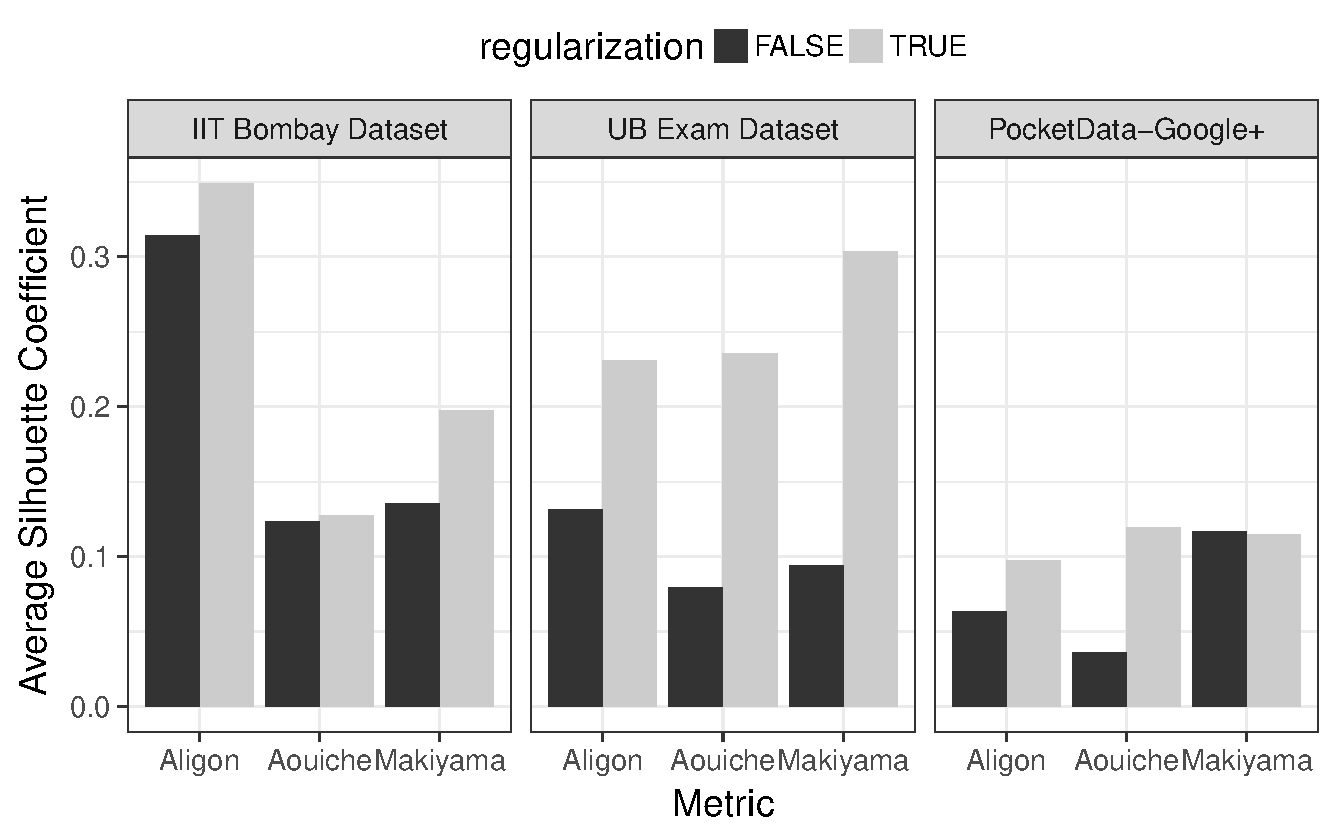
\includegraphics[width=\textwidth]{graphics/silhouette2}
        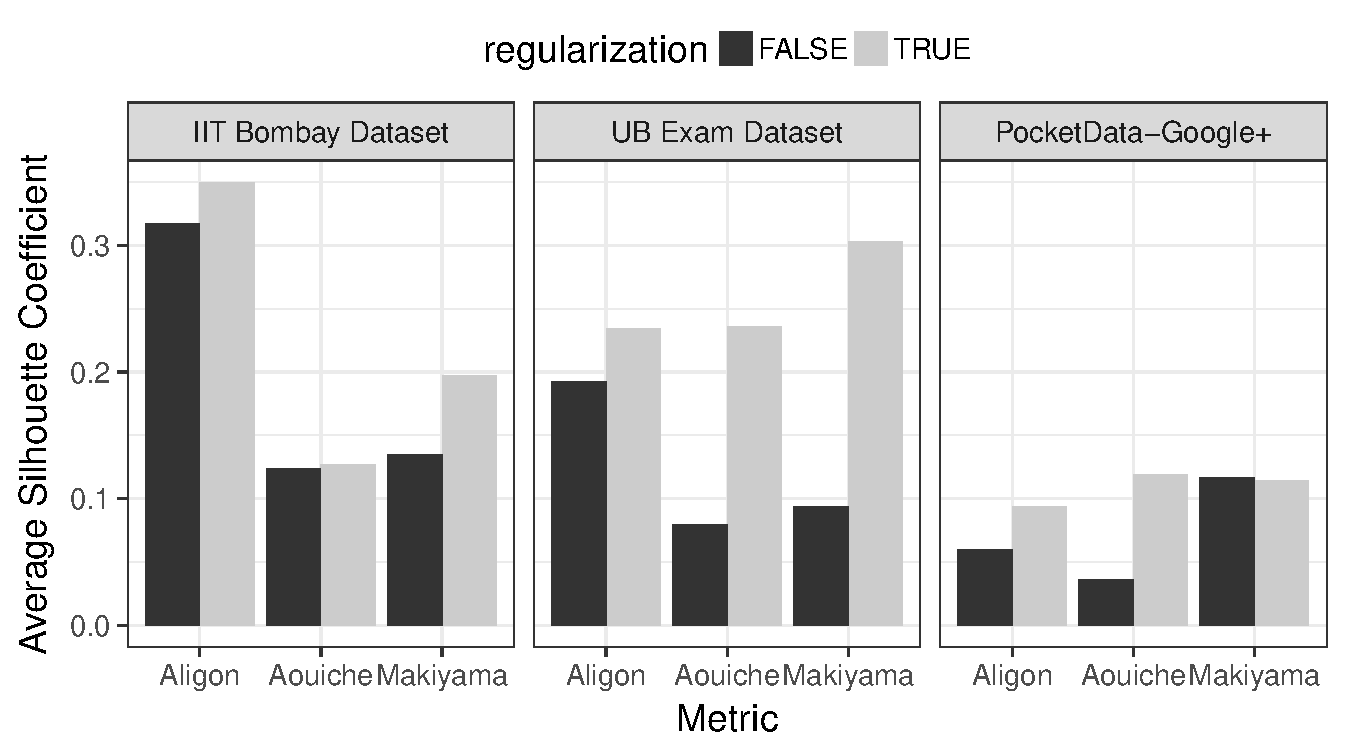
\includegraphics[width=\textwidth]{TKDE-QuerySimilarity/graphics/compare_silhouette}
        \caption{Average Silhouette Coefficient\\(\textit{larger} values are better)}
    \end{subfigure}%
    ~
    \begin{subfigure}[b]{0.48\textwidth}%{0.322\textwidth}
        \centering
        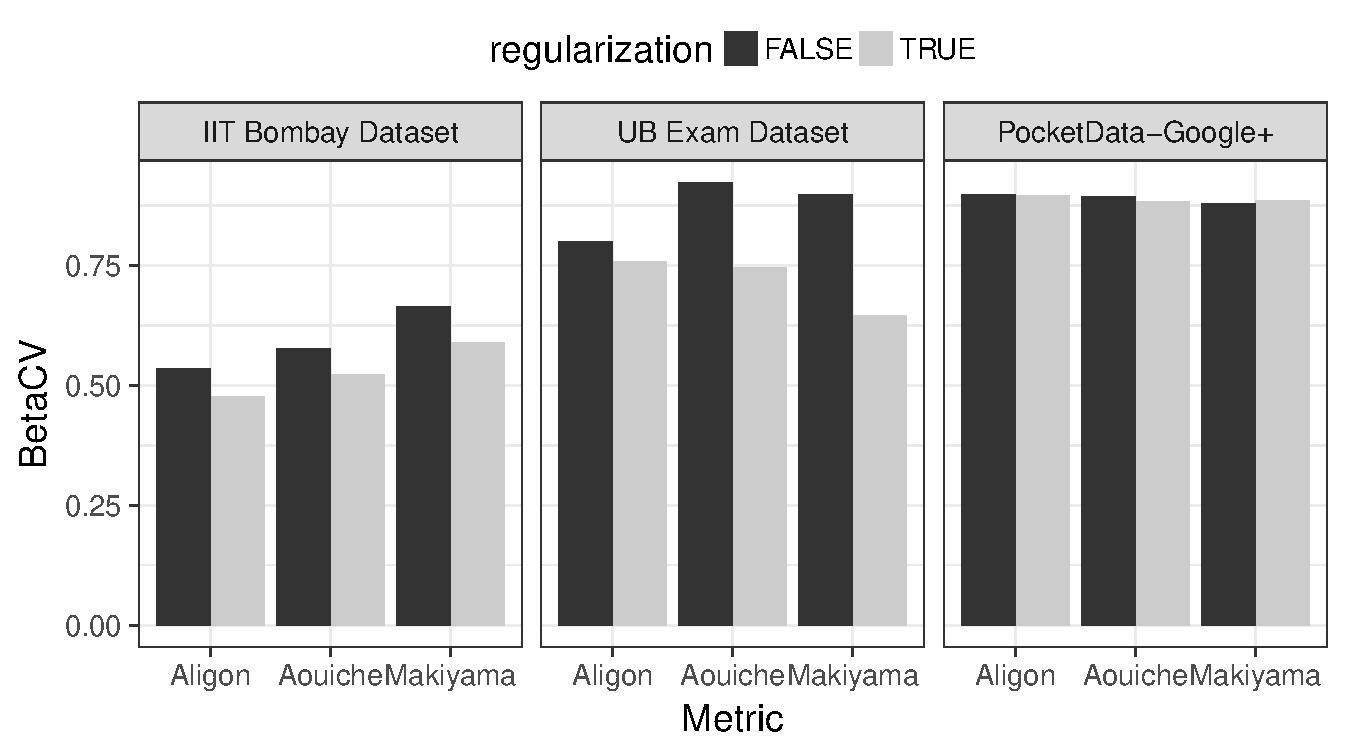
\includegraphics[width=\textwidth]{TKDE-QuerySimilarity/graphics/compare_betacv}
        \caption{BetaCV\\(\textit{smaller} values are better)}
    \end{subfigure}
    ~
    \begin{subfigure}[b]{0.48\textwidth}%{0.322\textwidth}
        \centering
        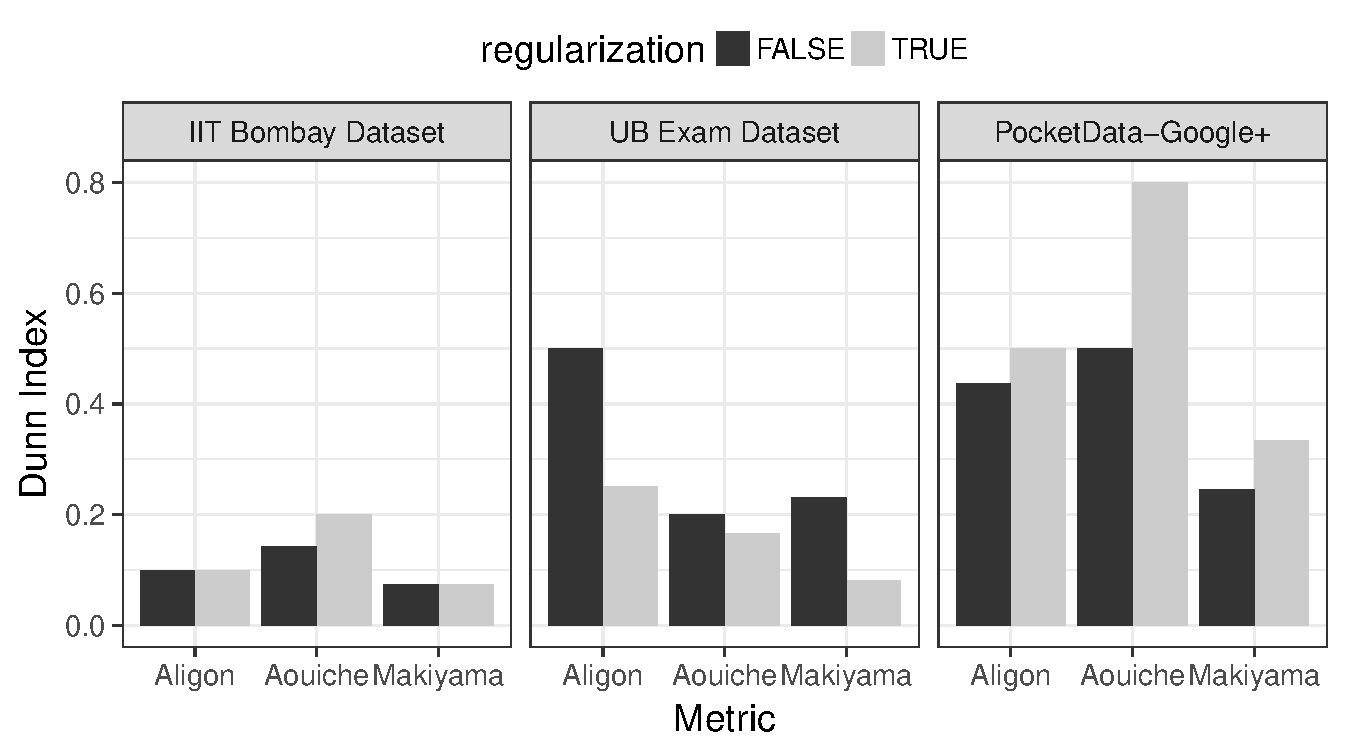
\includegraphics[width=\textwidth]{TKDE-QuerySimilarity/graphics/compare_dunn}
        \caption{Dunn Index\\(\textit{larger} values are better)}
    \end{subfigure}
    \caption{Clustering validation measures for each metric with and without regularization step}
    \label{fig:comparison2}
\end{figure*}

The black columns in Figure~\ref{fig:comparison2} show a comparison of three similarity metrics using each of the three quality measures (Average Silhouette Coefficient, BetaCV and Dunn Index).  
As can be seen in Figure~\ref{fig:comparison2}, Aligon seems to work the best for both IIT Bombay and UB Exam dataset while achieving second-best for PocketData-Google+ dataset under the Average Silhouette Coefficient measure. 
When considering BetaCV measure, Aligon also attains the best result for both IIT Bombay and UB Exam dataset while having comparable result for PocketData-Google+ dataset.
Aligon also performs well on the Dunn Index, coming in first on UB Exam dataset, and second-best for IIT Bombay and PocketData-Google+ dataset.
Especially given that the Dunn Index measures only worst-case performance, Aligon's metric seems to be ideal for our workloads.
This shows that even a fairly simple approach can capture task similarity well. 

\begin{figure*}[h!]
	\captionsetup[subfigure]{justification=centering}
    \centering
    \begin{subfigure}[b]{0.45\textwidth}%{0.32\textwidth}
        \centering
        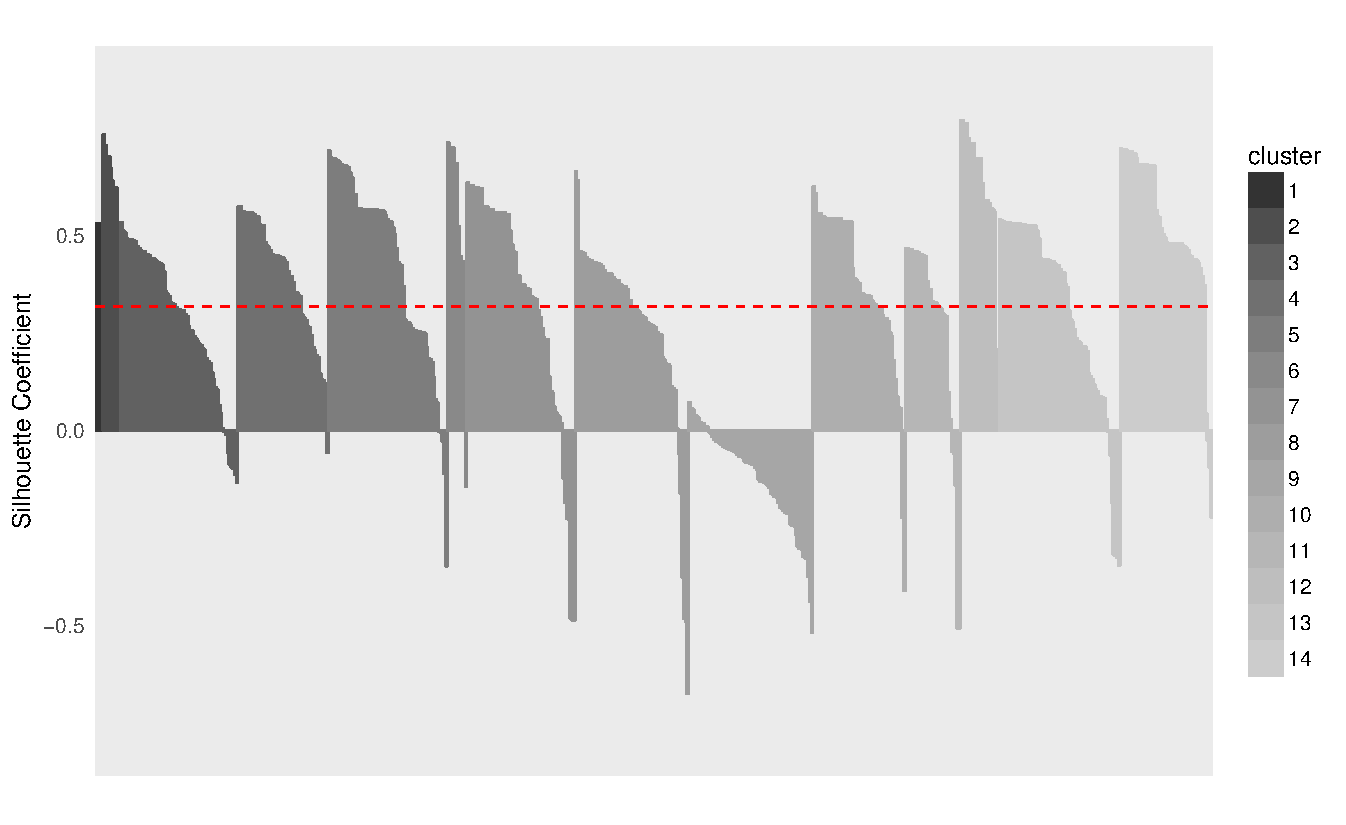
\includegraphics[width=\textwidth]{TKDE-QuerySimilarity/graphics/sil_bombay_Aligon}
		\caption{IIT Bombay dataset}
        \label{fig:sil_aligon:bombay}
    \end{subfigure}
    ~
    \begin{subfigure}[b]{0.45\textwidth}%{0.32\textwidth}
        \centering
        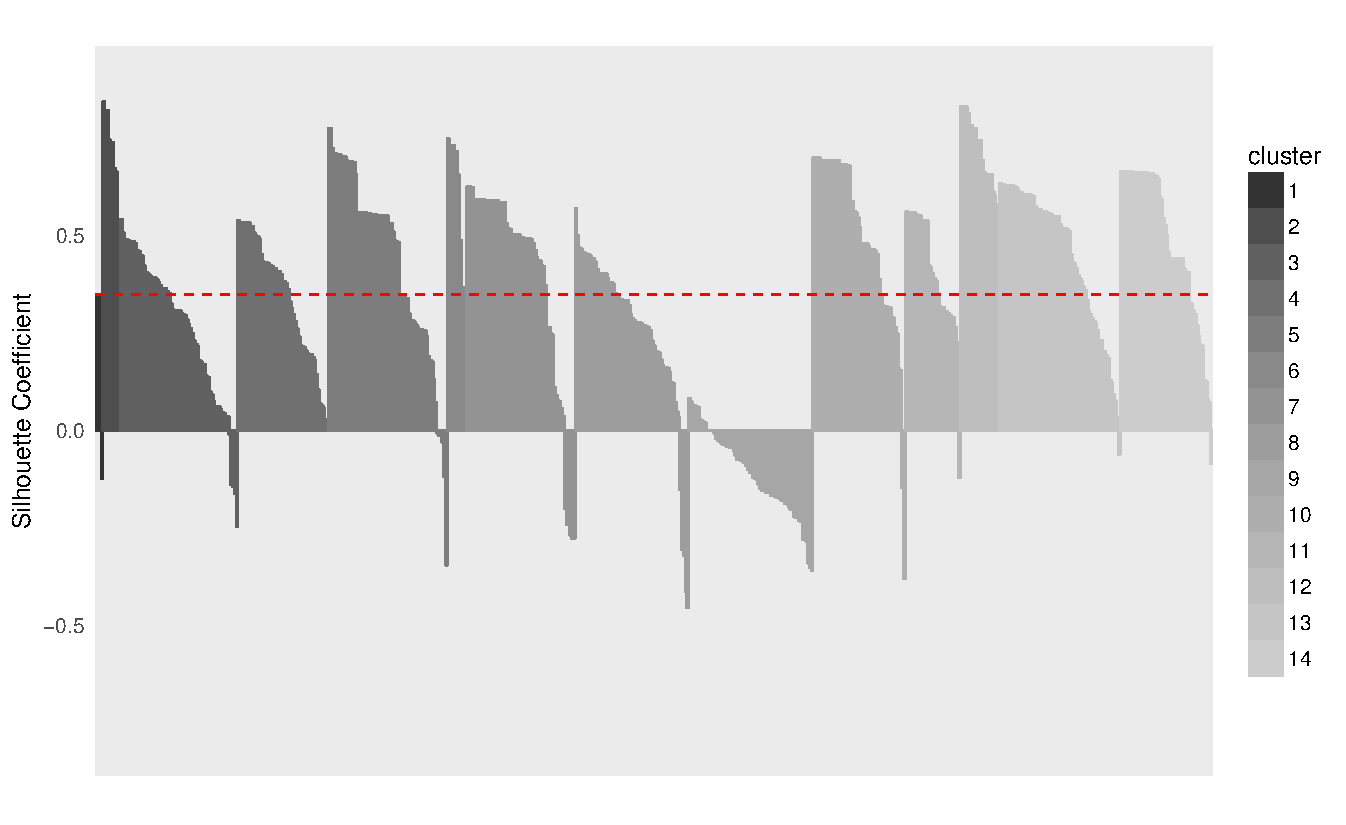
\includegraphics[width=\textwidth]{TKDE-QuerySimilarity/graphics/sil_bombay_Aligon_regularization}
		\caption{IIT Bombay dataset}
		\label{fig:sil_aligon:bombay_preprocess}
    \end{subfigure}
    \\
    \begin{subfigure}[b]{0.45\textwidth}%{0.32\textwidth}
        \centering
        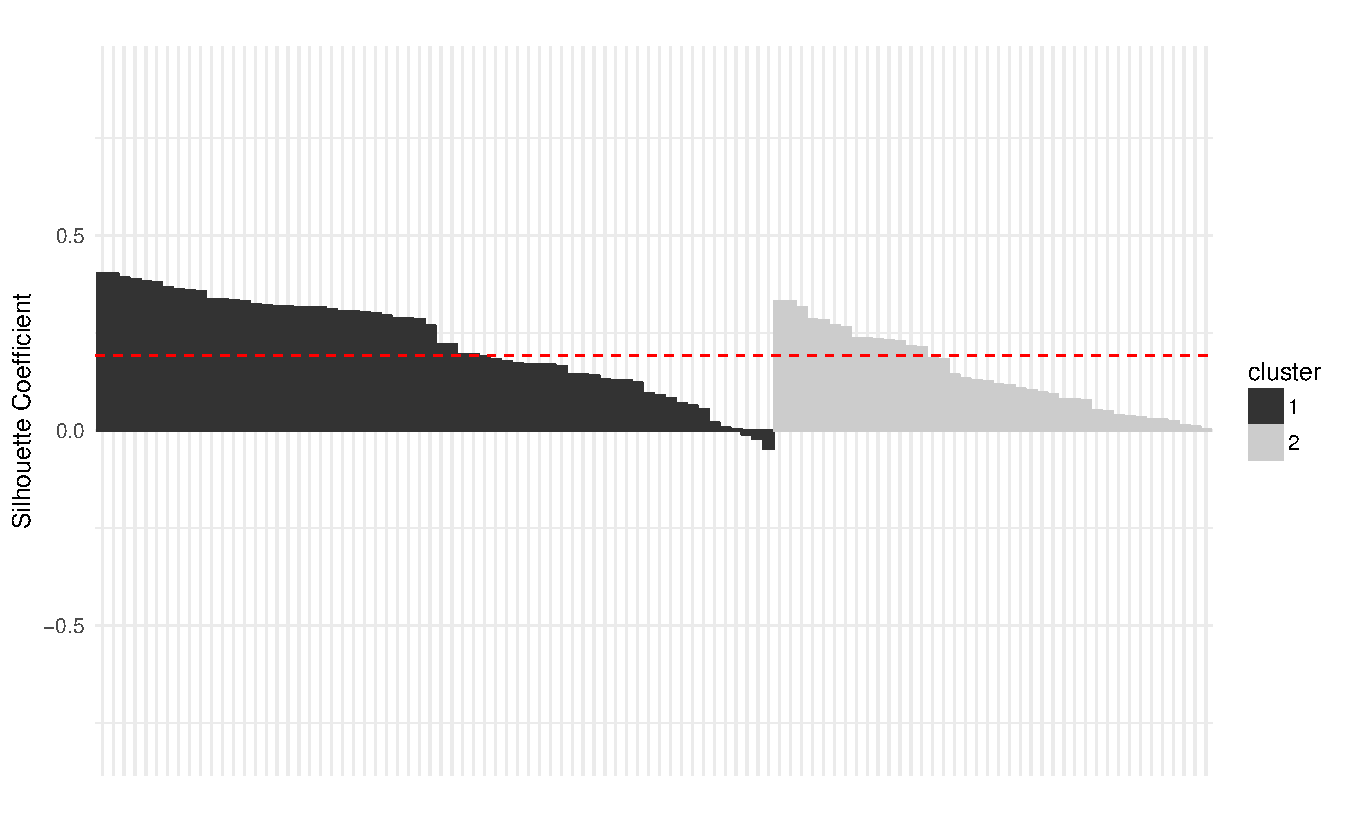
\includegraphics[width=\textwidth]{TKDE-QuerySimilarity/graphics/sil_ub_Aligon}
        \caption{UB Exam dataset}
        \label{fig:sil_aligon:local}
    \end{subfigure}
    ~
	\begin{subfigure}[b]{0.45\textwidth}%{0.32\textwidth}
        \centering
        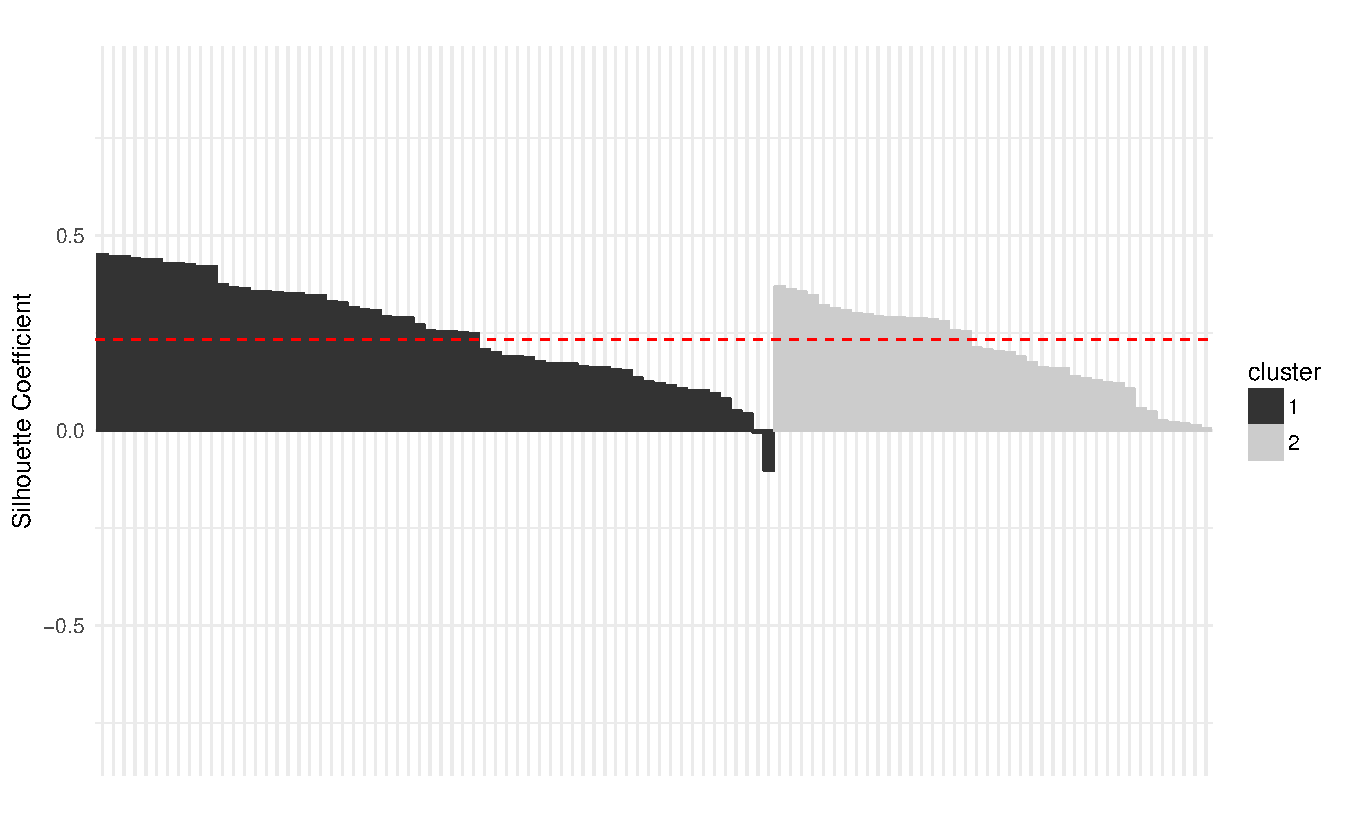
\includegraphics[width=\textwidth]{TKDE-QuerySimilarity/graphics/sil_ub_Aligon_regularization}
        \caption{UB Exam dataset}
        \label{fig:sil_aligon:local_preprocess}
    \end{subfigure}    
    \\
    \begin{subfigure}[b]{0.45\textwidth}%{0.32\textwidth}
        \centering
        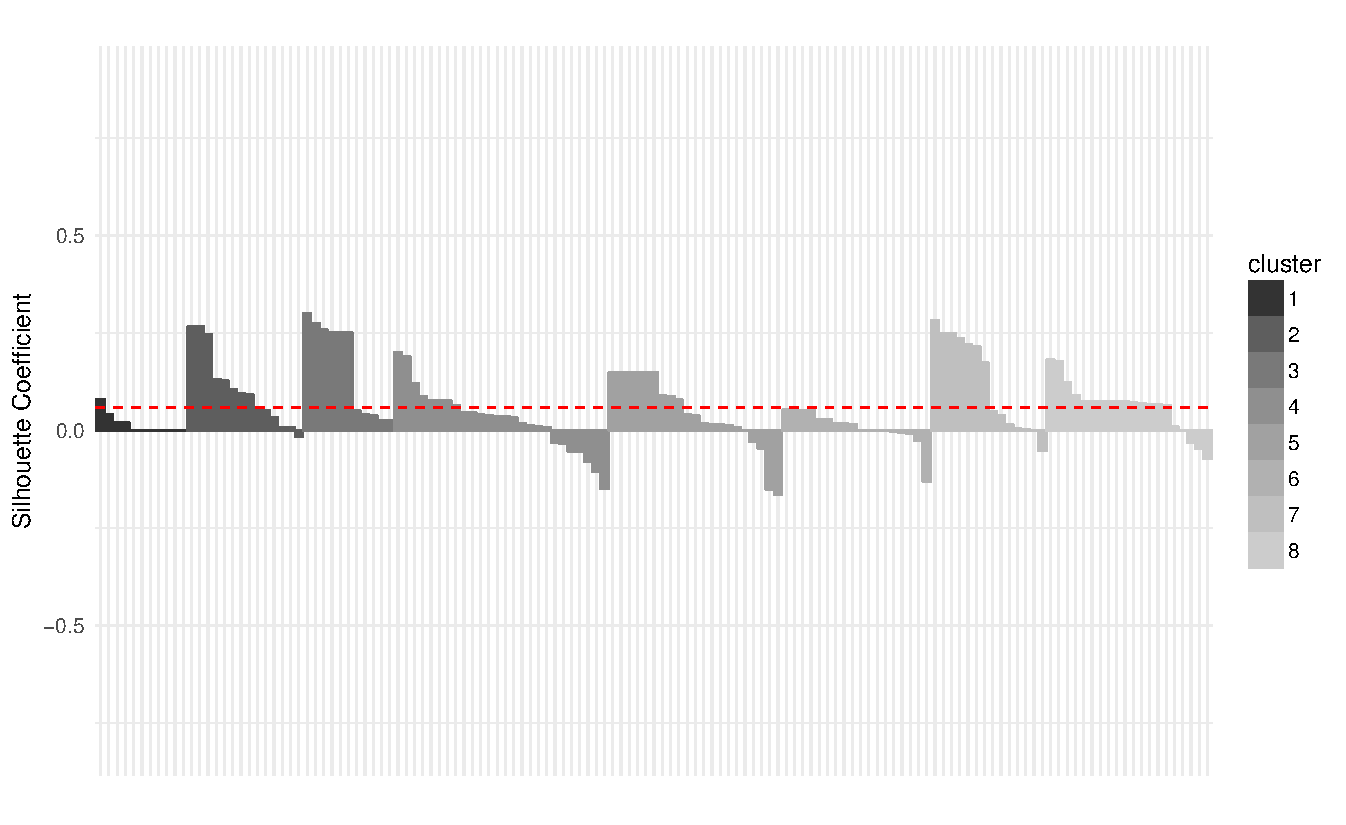
\includegraphics[width=\textwidth]{TKDE-QuerySimilarity/graphics/sil_googleplus_Aligon}
        \caption{PocketData-Google+ dataset}
        \label{fig:sil_aligon:googleplus}
    \end{subfigure}
    ~
    \begin{subfigure}[b]{0.45\textwidth}%{0.32\textwidth}
        \centering
        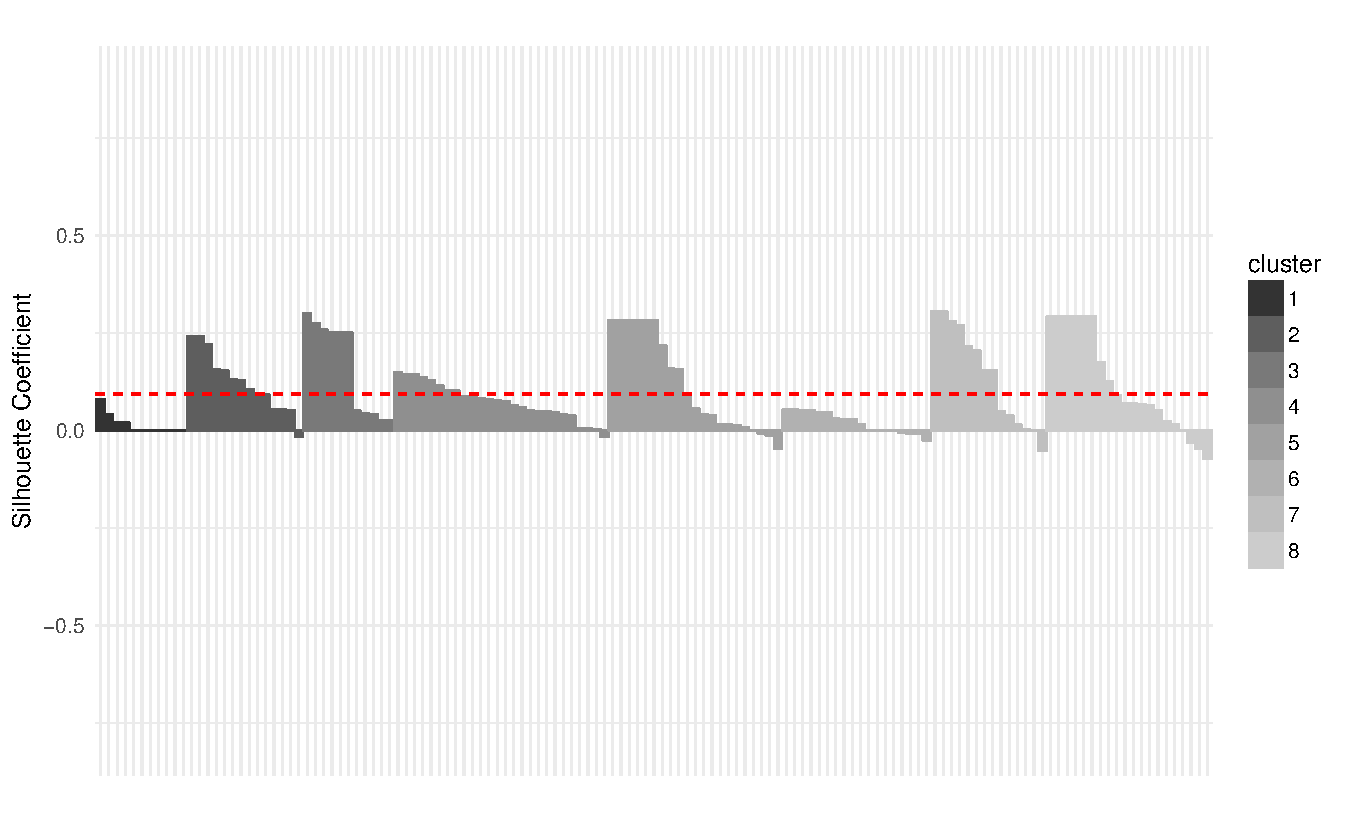
\includegraphics[width=\textwidth]{TKDE-QuerySimilarity/graphics/sil_googleplus_Aligon_regularization}
        \caption{PocketData-Google+ dataset}
        \label{fig:sil_aligon:googleplus_preprocess}
    \end{subfigure}
    \caption{Distribution of silhouette coefficients when using Aligon's similarity without regularization (a,c,e), and when regularization is applied (b,d,f)}
    \label{fig:sil_aligon}
    \label{fig:sil_aligon_preprocessed}
\end{figure*}

For a closer look of Aligon's similarity metric, Figure~\ref{fig:sil_aligon}(a,c,e) shows the distribution of Silhouette coefficients for each query and their respective tasks.   
Recall that the silhouette coefficient below 0 effectively indicates a query closer to another cluster than its own, or a query that would be mis-classified.  The further below zero, the greater the error.  
For the UB Exam dataset (Figure~\ref{fig:sil_aligon:local}), the majority of queries would have been successfully classified, and only a small fraction exhibit minor errors.
For the PocketData-Google+ dataset (Figure~\ref{fig:sil_aligon:googleplus}), there are some erroneous queries in cluster 4, 5 and 6 while cluster 1, 2, 3, 7 and 8 have very few errors.
For the Bombay dataset (Figure~\ref{fig:sil_aligon:bombay}), the distribution of errors varies.  
Cluster 1, 2, 4, 6, 12 and 14 exhibit virtually no error, while cluster 7, 8, and 9 exhibit particularly egregious errors.

\subsection{Evaluation of feature engineering}
\label{subsec:evaluation}
The effectiveness of regularization is evaluated by applying it to each of the three metrics described in Section~\ref{sec:background}.
The quality evaluation scheme is used to compare the quality of each measure both with and without feature engineering.

Figure~\ref{fig:comparison2} shows the values of three validation measures for each of the three similarity metrics, both with and without regularization.
As shown in Figure~\ref{fig:comparison2}, regularization significantly improves the Average Silhouette Coefficient and BetaCV measures for all similarity metrics except for the case of Makiyama similarity metric with PocketData-Google+ dataset.
The Dunn index is relatively unchanged or little improved for the IIT Bombay and PocketData-Google+ dataset and shows slight signs of worsening with regularization on the UB Exam dataset. To understand the reason of worse Dunn Index, Figure~\ref{fig:sil_aligon:local} (original) is compared with Figure~\ref{fig:sil_aligon:local_preprocess} (with regularization). 
The Silhouette Coefficient for answers that are originally positive in each question are considerably increased, and for answers that are originally negative (regarded erroneous) are even more decreased as a result of regularization, since it reduces the query structure diversity which leads to separating queries better.
In other words, for erroneous answers with negative Silhouette Coefficients, distance metrics like Aligon distinguish them further apart from answers with positive Silhouette Coefficients after regularization. 
Since erroneous answers are treated as the `worst cases' for each question, the Dunn Index which measures worst case performance naturally gets worse.

\subsubsection{Per-Query Similarity}
Figure~\ref{fig:sil_aligon_preprocessed}(b,d,f) shows the distributions of silhouette coefficients for the Aligon similarity metric after regularization is applied.  
For IIT Bombay dataset, comparing against Figure~\ref{fig:sil_aligon:bombay} there is a slight improvement at the tail end of clusters 9, 11, 12, 13 and 14 --- several of the negative coefficients have been removed.  
Furthermore, positive matches have been improved, particularly for cluster 7, 9, 10, 12 and 13.  
Finally, there has been a significant reduction in the degree of error in cluster 10.  
Cluster 10 is a particularly egregious case of aliasing, as the correct answer involves two self-joins in the same query.
As a result, aliasing is a fundamental part of the correct query answer, and our rewrites could not reliably create a uniform set of alias names.
In the UB Exam and PocketData-Google+ datasets, the improvement provided by regularization can be seen for queries with both positive and with negative values of $s(i)$.


\subsection{Case Study}
As part of the analysis, empirical explanations for query errors are provided by manual work, in particular for queries where $s(i) < 0$ for all three similarity metrics. 
Namely, queries that are too far apart from the clusters they belong are manually examined, and the reasons for mis-classification are categorized. 
We then investigate how the regularization process particularly affect these queries. 

Almost all of these egregiously mis-classified queries appear in the IIT Bombay dataset, the distribution of which is summarized in Table~\ref{tab:errorsources}.
The PocketData-Google+ dataset includes no egregiously mis-classified queries, while the UB Exam dataset includes only one such query (which tagged as a case of \textbf{Contextual equivalence}).
Each egregiously mis-classified query is tagged with an explanation that justifies why the query has a low s(i). 
Tags were drawn from the following list:

\smallskip
\tinysection{Ground-truth error} A student's response to the question may have been legitimately incorrect. This is a query that is correctly classified as an outlier.
For example: 
{\footnotesize
\begin{verbatim}
SELECT *
FROM (SELECT id, name, time_slot_id
 FROM (SELECT *
  FROM (SELECT *
   FROM student
    NATURAL JOIN takes) b1) a, section
   WHERE a.course_id = section.course_id) a1
\end{verbatim}
}
This query was attempting to complete the task \textit{``Find the ID and names of all students who have (in any year/semester) taken two courses in the same timeslot.''}

\smallskip
\tinysection{Nested subquery} A student's response is equivalent to a legitimately correct answer but uses nested subqueries such that a heuristic distance metric cannot recognize.
For example: 
{\footnotesize
\begin{verbatim}
SELECT id, name FROM student
WHERE id IN (SELECT DISTINCT s.id
 FROM (SELECT * FROM takes NATURAL JOIN section) s,
  (SELECT * FROM takes NATURAL JOIN section) t
 WHERE s.id = t.id
  AND s.time_slot_id = t.time_slot_id
  AND s.course_id <> t.course_id)
\end{verbatim}
}

Here, the subquery nesting structure is significantly different from other queries for of the same question.

\smallskip
\tinysection{Aliasing} Aliasing (e.g., \texttt{AS} in SQL) breaks a distance metric that relies on attribute and relation names.
For example:
{\footnotesize
\begin{verbatim}
SELECT DISTINCT student.id, student.name
FROM student, takes, section AS a, section AS b
WHERE student.id = takes.id
  AND takes.course_id = a.course_id
  AND takes.course_id = b.course_id
  AND a.course_id <> b.course_id
  AND a.time_slot_id = b.time_slot_id
\end{verbatim}
}

The student's use of \texttt{a} and \texttt{b} make this query hard to distinguish from other queries that may use other names for the attributes.

\smallskip
\tinysection{Insufficient features} Relevant query components are not sufficiently captured as features for a heuristic distance metric to distinguish between answers from sufficiently similar questions.

\smallskip
\tinysection{Too many features} Irrelevant query components create redundant features that artificially increase the distance between the query and cluster center.
For example:
{\footnotesize
\begin{verbatim}
SELECT DISTINCT student.name, takes.id, 
                s1.course_id, s2.course_id
FROM section AS s1, section AS s2, takes, student
WHERE takes.course_id = s1.course_id
  AND s1.course_id <> s2.course_id
  AND s1.time_slot_id = s2.time_slot_id
  AND s1.semester = s2.semester
  AND s1.year = s2.year
  AND takes.sec_id = s1.sec_id
  AND s1.semester = takes.semester
  AND s1.year = takes.year
  AND student.id = takes.id
  AND s2.time_slot_id = s2.time_slot_id
  AND takes.sec_id = s2.sec_id
  AND s2.semester = takes.semester
  AND s2.year = takes.year
\end{verbatim}
}

\smallskip
\tinysection{Contextual equivalence} Establishing query equivalence to properly clustered queries requires domain-specific knowledge not available to the distance metric (e.g. attribute uniqueness).
For example:
{\footnotesize
\begin{verbatim}
SELECT student.id, student.name
FROM student
WHERE student.id
  IN (SELECT takes.id
    FROM takes, section
    WHERE takes.course_id = section.course_id
      AND takes.sec_id = section.sec_id
      AND takes.semester = section.semester
      AND takes.year = section.year
    GROUP BY takes.id,
        takes.semester,
        takes.year,
        section.time_slot_id
    HAVING count(*) > 1)
\end{verbatim}
}

\begin{table}[h!]
%\vspace{-3mm}
\centering
\begin{tabular}{ccccccc}
\toprule
 \textbf{\begin{tabular}[c]{@{}c@{}}Cause\end{tabular}} & \textbf{\begin{tabular}[c]{@{}c@{}}Erroneous \\queries \\ Without \\ Regularization\end{tabular}} & 
 \textbf{\begin{tabular}[c]{@{}c@{}}Erroneous \\queries \\ With \\ Regularization\end{tabular}}\\
 \midrule
 All queries & 33 (100\%) & 27 (100\%)\\% & 1 (100\%) & 1 (100\%) & 0 (100\%)& 0 (100\%)\\  
 Ground-truth quality & 14 (42.4\%) & 14 (51.8\%)\\% & 0 (0\%) & 0 (0\%) & 0 (0\%) & 0 (0\%)\\ 
 Nested subquery & 7 (21.2\%) & 5 (18.5\%)\\% & 0 (0\%) & 0 (0\%) & 0 (0\%) & 0 (0\%)\\ 
 Aliasing & 8 (24.2\%) & 5 (18.5\%) \\%& 0 (0\%) & 0 (0\%) & 0 (0\%) & 0 (0\%)\\ 
 Insufficient features & 2 (6.0\%) & 1 (3.7\%)\\% & 0 (0\%) & 0 (0\%) & 0 (0\%) & 0 (0\%)\\ 
 Too many features & 1 (3.0\%) & 1 (3.7\%) \\%& 0 (0\%) & 0 (0\%) & 0 (0\%) & 0 (0\%)\\ 
 Contextual equivalence & 1 (3.0\%) & 1 (3.7\%)\\% & 1 (100\%) & 1 (100\%) & 0 (0\%) & 0 (0\%)\\
 \bottomrule
\end{tabular}
\vspace{-2mm}
\caption{Empirical error reasons for IITBombay Dataset}
\label{tab:errorsources}
%\vspace{-3mm}
\end{table}

Table~\ref{tab:errorsources} shows the primary reasons why these queries could not be classified correctly. 
Note that there may be more than one reason for a query to be placed in a different cluster, but in Table~\ref{tab:errorsources}, only the empirically determined primary reason is given.

Many of the queries with low silhouette coefficients are identified as incorrect answers for the task given. 
These answers directly affect the ground-truth quality, therefore reduce the average silhouette coefficient. 
Another reason for erroneous queries with low silhouette coefficients is because of aliasing. 
Although it is convenient for user to use aliases in the query to refer to a particular item, it is difficult for a machine to approximate the tasks the query authors are trying to accomplish since different query authors have different ways to name particular items in the query. 
This problem is particularly prevalent in question 9 of the IIT Bombay dataset.

Although the distribution of the error reasons are expected to change, all the tags provided in this section can generically be applied to other query logs given a ground-truth. 
The regularization method cannot be expected to fix errors originating from mis-classifications in ground-truth since they do not actually share any similarities with the cluster. 

After the regularization process, the silhouette coefficient under all three similarity metrics for each query is computed again and the result yields an 18\% overall reduction in number of erroneous queries ($s(i) < 0$)  in the IIT Bombay dataset. 

\subsection{Analysis of regularization by module}
\label{subsec:modules}
In subsection~\ref{subsec:evaluation}, the overall effect of regularization on query similarity is analyzed.  
However, as described in Section~\ref{sec:system}, regularization is composed of many different transformation rules.  
In this experiment, these rules are grouped into four separate modules before their impact on the clustering quality is inspected. 
One may observe that Commutative Operator Ordering is guaranteed to provide benefit in structure similarity comparison, hence it is included in all four modules. 
In addition, there are dependencies between rules that require them to operate one before another. 
For example, one should better apply Syntax Desugaring and then DNF Normalization to simplify the boolean expression in WHERE clause before OR-Union Transformation.
As another example, Exists Standardization should better be applied on nested sub-queries before we de-correlate them using Nested Query De-correlation.
As a result, the rules are grouped from Section~\ref{sec:system} into four modules:
\begin{enumerate}
\item \textit{Naming}: \textbf{Canonicalize Names and Aliases}
\item \textit{Expression Standardization}: \textbf{Syntax Desugaring}, \\\textbf{Exists~Standardization}, \textbf{DNF~Normalization}, \\\textbf{Nested~Query~Decorrelation}, \textbf{OR-Union~Transform}
\item \textit{FROM-Nesting}: \textbf{Flatten FROM-Nesting}
\item \textit{Union Pullout}: \textbf{OR-UNION Pullout}
\end{enumerate}
\textbf{Commutative Operator Ordering} is included in all modules.

Figure~\ref{fig:module} provides a comparison of each module in regularization. 
From this figure, one can observe that, since students use different names/aliases for their convenience when constructing queries, the \textit{Naming} module is the most effective one in terms of improving clustering quality for IIT Bombay and UB Exam datasets. 
On the other hand, for PocketData-Google+ dataset, names are already canonicalized as they are machine-generated. 
In this case, \textit{Expression Standardization} seems to be the most effective module, especially when using Aligon or Aouiche as similarity metric. 
In PocketData-Google+ dataset, referred tables and boolean expressions in the queries are both informative in distinguishing between different query categories or clusters. For this reason, Makiyama similarity metric which considers both works well even without regularization while Aligon and Aouiche can get commensurate performance only after applying \textit{Expression Standardization} module. 

Note that in Figure~\ref{fig:module}, \textit{Expression Standardization} makes Average Silhouette Coefficient worse in some cases for IIT Bombay and UB Exam data sets. 
The performance degradation is majorly due to \textit{feature duplication}. 
More specifically, consider the example query with \textit{Expression Standardization}.
\begin{example}
Syntax Desugaring with OR-UNION transform
{\footnotesize
\begin{enumerate}
\item\begin{verbatim}
SELECT name FROM usr WHERE 
rank IN {'admin','normal'}
\end{verbatim}
\item\begin{verbatim}
SELECT name FROM usr WHERE 
rank = 'admin' OR rank = 'normal'
\end{verbatim}
\item\begin{verbatim}
SELECT name FROM usr
WHERE rank = 'admin'
UNION
SELECT name FROM usr
WHERE rank = 'normal' 
\end{verbatim}
\end{enumerate}
}
\end{example}
Query (1) is transformed into (2) by syntax~desugaring and then into (3) by OR-UNION~Transform. From (1) to (2), feature \texttt{WHERE rank} has been replicated; From (2) to (3), features \texttt{SELECT name} and \texttt{FROM usr} have been duplicated. For expressions of the form: \texttt{X IN} $\{x_1,x_2,\dots,x_n\}$, feature duplication becomes dominant when $n$ grows large. 
In Figure~\ref{fig:module}, Aligon and Makiyama suffer from feature duplication brought by~\textit{Expression Standardization} in some cases while Aouiche does not. 
Because Aouiche records feature existence instead of occurrence in its vector. 
Although in some cases such as this, simply replacing feature occurence with existence solves the problem of feature duplication, feature occurence can also be a good indicator for the interests of the query. 
It is believed that this problem can be addressed with exploration of feature weighting strategies. 
Therefore, the problem of feature duplication will be further explored as a part of feature weighting strategies in our future work.

\begin{figure*}[h!]
    \vspace*{-2mm}
    \centering
    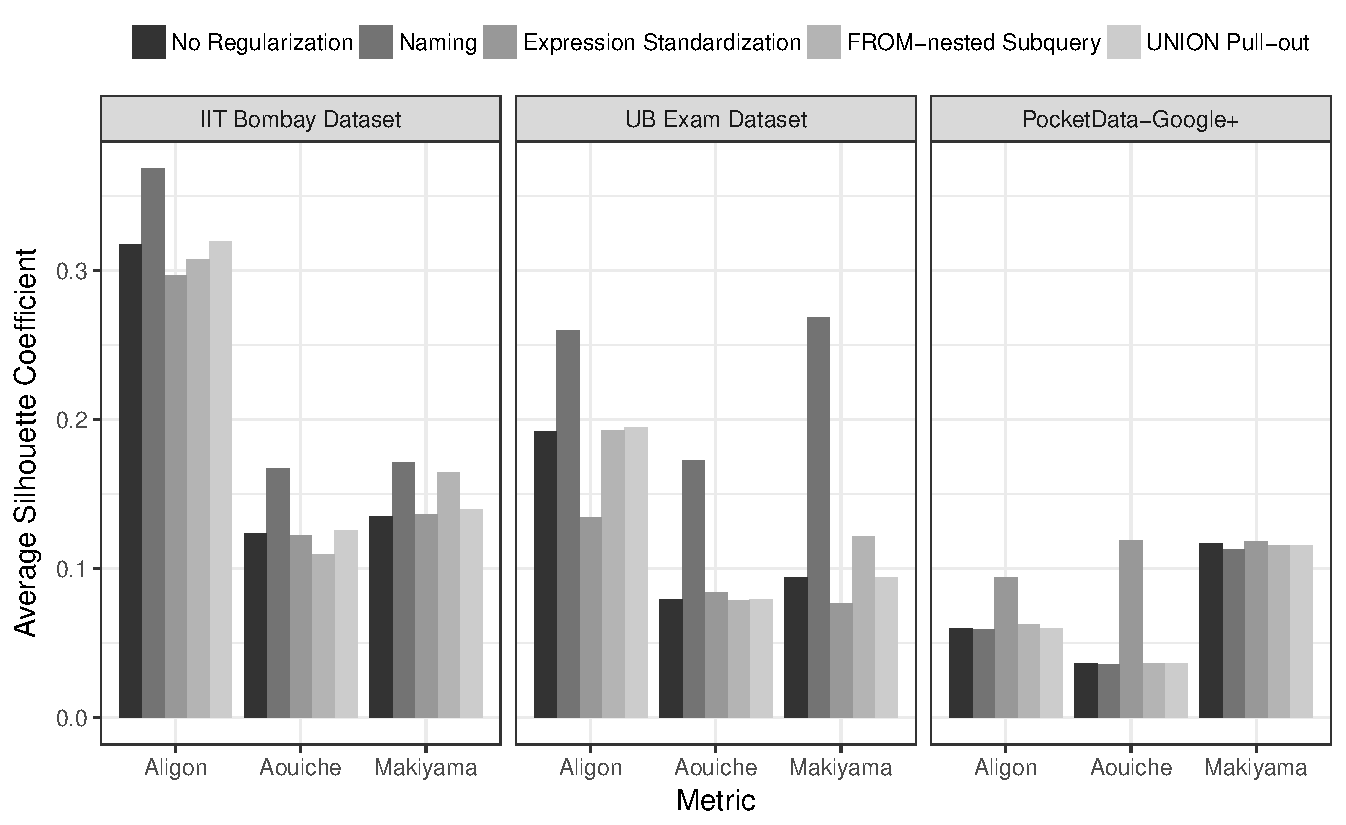
\includegraphics[width=0.70\textwidth]{TKDE-QuerySimilarity/graphics/module}%[width=\columnwidth]{graphics/module}
	\caption{Effect of each module in regularization}
    \label{fig:module}
    %\vspace*{-4mm}
\end{figure*}



\section{Discussion}
\label{sec:discussion}
% !TEX root = ../paper.tex
%This paper presents the first steps for \sysname{}.
We have reviewed several similarity metrics for clustering queries and focused on three syntax-based methods that offer an end-to-end similarity metric. The advantage of this preference is that, syntax-based methods do not require access to the data in the database or database properties. Considering that only logs are usually transferred between organizations, and requiring access to the data for investigations can cause privacy violations, we preferred focusing on the syntax-based approach.

The survey we performed shows that most of the metrics make use of selection and join operations in the queries and consider them as the most important items for similarity calculation. Group-by aggregate follows them closely while projection items take the third most important item set. There are other possible feature sets that can be used, such as tables accessed or the abstract syntax tree (AST) of a query, but these feature sets are generally overlooked.

%We have surveyed and measured the evaluation of query similarity metrics for clustering similar queries together and picked three methods that offer an end-to-end similarity metric. The survey shows that most of the metrics make use of selection and join predicates and consider them the most important items for similarity comparison. Group-by predicates follows them closely while projection items take the third most important item set. There are other possible feature sets that can be used in queries like the tables accessed or the AST of a query, but these feature sets are generally overlooked.

%As shown in Figure~\ref{fig:comparison1}, apart from the Dunn index value for IIT Bombay dataset, Aligon \textit{et al.}~\cite{aligon2014similarity} performs the best amongst the surveyed methods.
% All the approaches surveyed can provide the user with an immediate view on the quality of their clustering. 
%The success of this method can be attributed to the choice of the feature set: selection, joins, group by and projection items separately have their own weightings in the general calculation of the similarity.
Although Aouiche \textit{et al.}~\cite{aouiche2006}
%have a similar strategy; making
make use of the most important features selection, joins, and group-by items, they don't utilize the number of times an item appears, or after the parsing, they don't consider what kind of feature an item is. This means, it does not matter if a query has \texttt{rank} column in group-by, and the other one has \texttt{rank} column in selection; they are considered the same. Makiyama \textit{et al.}~\cite{makiyama2015text}, on the other hand, follow Aligon \textit{et al.}~\cite{aligon2014similarity} in separating the different features, and improves on it by making use of appearance count of items. However, while trying to make use of every item like \texttt{FROM} and \texttt{Order-By} predicates, they consider these low priority predicates with same importance as the selection and join predicates.

Makiyama \textit{et al.}~\cite{makiyama2015text} use a more complete structure of the query AST, hence when the query is simple like in the PocketData-Google+ dataset, this technique can be slightly better.
However, for a complex query with redundant features, mixing features captured from various components of a query without proper feature re-weighting will essentially decrease the weight of features that are more informative.
Hence, in student exam datasets, we can observe that Aligon \textit{et al.}~\cite{aligon2014similarity} is better than the others while in PocketData-Google+ dataset, Makiyama \textit{et al.}~\cite{makiyama2015text} is better.

We could further improve these methods by making use of the abstract syntax tree (AST) of a SQL statement.
As a declarative language, the AST of a SQL statement acts as a proxy for the task of the query author.
This suggests that a comparison of ASTs can be a meaningful metric for query similarity.
For instance, we can group a query $Q$ with other queries that have nearly (or completely) the same AST as $Q$.
This structural definition of task has seen substantial use already, particularly in the translation of natural language queries into SQL~\cite{li2015NLPI}.
For two SQL queries $Q_1$ and $Q_2$, one reasonable measure might be to count the number of connected subgraphs of $Q_1$ that are isomorphic to a subgraph of $Q_2$.  
Subgraph isomorphism is NP-complete, but a computationally tractable simplification of this metric can be found in the Weisfeiler-Lehman (WL) Algorithm~\cite{WL2011, kul2016ettu}.

As can be seen in Tables~\ref{tab:xdata} and \ref{tab:ub_exam}, as the complexity or difficulty of the question increases, the number of distinct queries also increases, i.e., students find different ways to solve the same problem.
Especially, in Table~\ref{tab:ub_exam}, no two students answer a question using the same structure.
This phenomenon motivates the need for regularization in comparing SQL queries.
As the complexity of the query increases, the possible ways to create the query to achieve the same task increase.
Figure~\ref{fig:comparison2} shows that our assumption that regularizing queries will improve overall clustering quality is correct.
Our proposed feature engineering scheme improves the overall clustering quality of all three metrics on all three datasets, including both human- and machine-generated queries.

%One caveat is that regularization is only suitable for query comparison purpose as some of its transformations do not retain equivalence.
%In addition, once a nested sub-query is flattened and merged with its parent, aliases in the parent query pointing to it become invalid.
%At the same time, names across different query bodies are merged and name uniqueness is not guaranteed any more.
%Skewed names in the query will make query comparison error-prone.

%Although we run our experiments on a multi-core server, our implementations are single-threaded.
%We believe that modifying our algorithms to run parallel can significantly decrease the running time.

%Hence we apply a recommended step before regularization that renames all entities in the query containing aliases. 

%In Section~\ref{sec:WL}, we introduce a new similarity metric that is based on the feature extraction scheme based on the Weisfeiler--Lehman test of isomorphism on graphs where we make use of query ASTs instead of atomic features. Even with this naive approach, the performance of the metric is competitive with the metrics surveyed in this paper as can be seen in Figure~\ref{fig:comparison3}. The quality is further improved with the regularization scheme we proposed as shown in Figure~\ref{fig:comparison4}.  Furthermore, the algorithm can be benefit greatly from feature weighting (e.g. appointing higher weights to the features created from selection and joins) and dimensionality reduction with PCA, ICA or other feature selection techniques. Just like Makiyama \textit{et al.}~\cite{makiyama2015text}, we create many unimportant features along with the important ones, and feature selection can improve the accuracy of the metric greatly.


\section{Application Scenarios}
\label{sec:scenarios}
%!TEX root = ./sections/1-intro.tex
In this section, three scenarios are provided where the clustering scheme coupled with the proposed regularization is applicable:

The first one is, \textit{Jane the DBA} where she takes on the task of improving database performance.
After performing the straightforward database indexing tasks, she would need to select candidate \textit{views}, which are virtual tables defined by a query.
They allow querying just like tables by pre-fetching records from existing tables. 
Constructing a view for a frequent complex join operation can increase querying performance of the database substantially.
To find the ideal views, Jane first clusters similar queries together to see what kinds of queries are more frequent.
Making the most frequent complex query types faster by creating views of them could improve database performance substantially~\cite{aouiche2006, aligon2014similarity}. 

The second one is, \textit{Jane the security auditor} where she suspects that there is a person who leaks classified information from her organization.
She can choose to investigate database access patterns along with other strategies which would involve query clustering~\cite{Sun2016}.
After identifying the query clusters, she can partition the queries by the department or role to get the intuition about which departments and roles \textit{normally} utilize what part of the database.
She can detect the \textit{outliers} from that behavior in order to determine the suspects for further investigation.

Lastly, \textit{Jane the researcher} where needs to investigate the properties of the SQL query dataset that she is going to use for her research.
One of the new graduate students in her team clusters the queries, and provides her with the clustering assignments of each query.
She doubts the quality of the clustering performed, and wonders if the clustering operation could be performed better.

Having a \textit{better} clustering of queries would potentially enhance the quality of her work in all of the examples given above.
Also, works cited in this section~\cite{aouiche2006, aligon2014similarity, Sun2016}, along with many others can benefit from the framework described in this chapter.


%\section{Conclusion and Future Work}
%\label{sec:conclusion}
%% !TEX root = ../paper.tex
The focus of this work is to understand and improve similarity metrics for SQL queries relying on query structure to be used to cluster queries. 
We described a quality evaluation scheme that captures the notion of query task using student answers to query-construction problems and a real-world smartphone query load.
We used this scheme to evaluate three existing query similarity metrics.
We also proposed a feature engineering technique for standardizing query representations.
Through further experiments, we showed that different workloads have different characteristics and no one similarity metric surveyed was always good. 
The feature engineering steps provided an improvement across the board because they addressed the error reasons we identified. 

The approaches described in this article only represent the first steps towards tools for summarizing logs by tasks.
Concretely, we plan to extend our work in several directions:
First, we will explore new feature extracting mechanisms like the Weisfeiler-Lehman framework~\cite{kul2016ettu}, feature weighting strategies and new labeling rules in order to capture the task behind logged queries better.
Second, we will introduce the temporal order of the log to increase the query clustering quality. In this article, we focused on query structures to improve clustering quality. Exploring the inter-query feature correlation based on query order can be used to summarize query logs in addition to clustering.
Third, we will examine user interfaces that better present clusters of queries --- Different feature sorting strategies in Frequent Pattern Trees (FP Trees)~\cite{han2004mining} in order to help the user distinguish important and irrelevant features, for example.
Lastly, we will investigate the temporal effects on query clustering. 

\chapter{Application: Interactive Semi-Structured Schema Design}
\section{Introduction}
\label{sec:introduction}
% -*- root: ../cnf-json.tex -*-

Semi-structured formats like \json allow users to design schemas on-the-fly, as data is generated.
For example, adding a new attribute to the output of a system logger does not break backwards compatibility with existing data.
This flexibility facilitates the addition of new features and enables low-overhead adaptation of data-generating processes.
However, because the data does not have a consistent underlying schema, it can be harder (and slower) to explore than simple tabular data.
The logic of each and every query must explicitly account for variations in the schema like missing attributes.  
Performance also suffers, as there is no one physical data representation that is ideal for all schemas.

To address these problems, a variety of techniques~\cite{DBLP:conf/cidr/LiuG15,DBLP:conf/edbt/BaaziziLCGS17,DBLP:conf/sigmod/DiScalaA16,DBLP:conf/vldb/GoldmanW97,spoth:2017:cidr:adaptive} have arisen to generate schemas after-the-fact.
The goal of these \emph{semi-structured schema discovery} (\sssd) techniques is to propose a schema for collections of \json records.
A common approach to this problem is to bind the \json records to a normalized relational representation, or in other words, to derive a set of flat \emph{views} over the hierarchical \json data.

Existing automated approaches to this problem (e.g., \cite{DBLP:conf/sigmod/DiScalaA16,DBLP:conf/vldb/GoldmanW97}) operate in a single-pass: They propose a schema and consider their job done.
Unfortunately these techniques also rely heavily on general heuristics to select from among a set of schema design choices, as a clear declarative specification of a domain would be tantamount to having the schema already.
To supplement domain-agnostic heuristics with feedback from domain experts, we propose a new \emph{iterative and interactive} approach to \sssd called \systemnametwo.

\systemnametwo provides a OLAP-style interface (with analogs to roll-up, drill-down, and slice+dice) specialized for exploring collections of \json records.  
Every state of this interface corresponds to a relational view defined over the \json data.
When ready, this view can be exported to a classical RDBMS or similar tool for simplified, more efficient data access.
In this paper, we explore several design options for \systemnametwo, and discuss how each interacts with the challenges of \sssd.

\subsection{Extracting Relational Entities}
The first class of challenges we address involve the nuts and bolts of mapping hierarchical \json schemas to flat relational entities.  
Fundamentally, this involves a combination of three relational operators: Projection, Selection, and Unnesting.  

\tinysection{Projecting Attributes}
\json schema discovery can, naively, be thought of as a form of schema normalization~\cite{Codd:1979:EDR:320107.320109}, where each distinct path in a record is treated as its own attribute.
Entities then, are simply groups of attributes projected out of the \json data, and 
the \sssd problem reduces to finding such groups (e.g., by using Functional Dependencies~\cite{DBLP:conf/sigmod/DiScalaA16}).  

\tinysection{Selecting Records}
This naive approach fails in situations where the collection of \json records is a mix of different entity types that share properties.
As a simple example, Twitter streams mix three entity types: tweets, retweets, and deleted tweets.  
Although each entity appears in distinct records, they share attributes in common.
Hence, entity extraction is not just normalization in the classical sense of partitioning attributes, but rather also a matter of partitioning records by content.

\tinysection{Collapsing Nested Collections}
\json specifies two collection types: Arrays and Objects.  
Typically the former is used for encoding nested collections and the latter for encoding tuples with named attributes.
However, this is not a strict requirement.
For example, latitude and longitude are often encoded as a 2-element array.
Conversely, in some data sets, objects are used as way to index collections by named keys rather than by positions.
Hence, simple type analysis can not distinguish between the two cases.
This is problematic because treating a collection as a tuple creates an explosion of attributes that make classical normalization techniques incredibly expensive.

\subsection{Human-Scale \sssd}
Even in settings where \json data is comparatively well behaved, it is common for it to have dozens, or even hundreds of attributes per record.  
Similarly, individual \json records can be built from any of the hundreds or thousands (or more) different permutations of the full set of attributes used across the entire collection.
Bringing this information down to human scale requires simultaneously simplifying and summarizing.

\tinysection{Summarization}
For the purposes of entity construction, the full set of attributes is often unnecessary.
It is often possible to collapse multiple attributes together, or express attributes as equivalent alternatives.
As an example, an address might consist of four distinct attributes city, zip code, street, and number when it could conceptually be expressed as just one.

\tinysection{Visualization}
In addition to simplifying the underlying problem, it is also useful to give users a coarse ``top-down'' view of the schema process.
Specifically, users need to (1) be able to see patterns of structural similarity between distinct schemas, and (2) understand how much variation exists in the data set as-is.

\tinysection{Iteration}
By combining straightforward summarization and data visualization techniques, \systemnametwo helps users to quickly identify natural clusters of records and attributes that represent relational entities.
\systemnametwo facilitates an \emph{iterative} schema design process to allow human experts to better evaluate whether structures in the data indicate conceptual relationships between records or attributes, or are merely data artifacts.

\begin{figure}
\centering
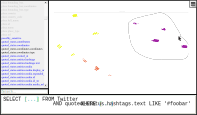
\includegraphics[width=0.9\linewidth]{SchemaSummarization/img/UI}
\caption{Prototype user interface for \systemnametwo.}
\label{fig:ui}
\end{figure}

\subsection{Overview}
Figure~\ref{fig:ui} shows the prototype interface of \systemnametwo. 
The pane on the left, discussed in Section~\ref{sec:distribution}, shows the schema of the currently selected JSON view, highlighting attributes and groups based on relevance.
The pane on the right, discussed in Section~\ref{sec:visualization}, provides a top-down visual sketch of schemas in the currently selected JSON data, and allows users to interactively filter out parts of it.
Finally in Section~\ref{sec:visualization}, we show examples of how \systemnametwo facilitates incremental, iterative exploration and mapping of JSON schemas.






\section{Summarization}
\label{sec:distribution}
% !TEX root = ../cnf-json.tex
The first component of \systemnametwo, the schema pane, shows the relational schema of the extracted view.
Initially, this schema consists of one attribute for every path in the \json collection being summarized.
Attributes may be deleted or restored, and sets of attributes may be unified.

The core challenge behind implementing this pane is that, depending on data set, the schema could consist of hundreds or thousands of attributes.
This can be overwhelming for users who just wants to find account profiles appearing in a Twitter stream.
To mitigate this problem, \systemnametwo presents the schema in a summarized form.

Specifically, attributes are grouped based on both correlations and anti-correlations between them.
Groups of \emph{correlated} attributes, or those that frequently co-occur in \json records are likely to be part of a common structure.
Similarly, groups of \emph{anti-correlated} attributes, or those that rarely co-occur in \json records are likely to represent alternatives (e.g., a Street Address vs GPS coordinates).  
We use correlations and anti-correlations between attributes to compact the schema for representation.
Before describing the summary itself, we first formalize the problem.

%%%%%%%%%%%%%%%%%%%%%%%%%%%%%%%%%%%%%%%%%%%%%%%%%%%%%%%%%%%%%%%%%%%%

\subsection{Data Model}
A \json object is an order-independent mapping from keys to values.
A key is a unique identifier of a \json object, typically a string.
A value may be atomic or complex. 
Atomic values in \json may be integers, reals, strings, or booleans.
A complex value is either a nested object, or an \textit{array}, an indexed list of values.  
For simplicity, we model arrays as objects by treating array indexes as keys.
A \json record may be any value type, but for simplicity of exposition we will assume that all records are objects.  
\begin{example}
\label{example:jsonobject}
A fragment of Twitter Tweet encoded as \json
\begin{lstlisting}[language=json]
"tweet": {
  "text": "#SIGMOD2018 in Houston this year",
  "user": { 
    "name" : "Alice Smith",  "id" : 12345, 
    "friends_count": 1023,  …
  },
  "retweeted_status": {
    "tweet": {
      "user": { … }, "entities": { … }, 
      "place": { … }, "extended_entities": { … }
    }, …
  },
  "place": { … }, "extended_entities": { … },  
  "entities": { "hashtags": [ "SIGMOD2018" ], … },
  …
}
\end{lstlisting}
\end{example}

\noindent 
\json objects are typically viewed as trees with atomic values at the leaves, complex values as inner nodes, and edges labeled with the keys of each child.
Our goal is to identify commonalities in the structure of this tree across multiple \json records in a collection.  
To capture the structure, we define the \textit{schema} $S$ of a \json record as the record with all leaf values replaced by a constant $\bot$.
A \emph{path} $P$ is a sequence of keys $P = (k_0, \ldots, k_N)$.
For convenience, we will write paths using dots to separate keys (e.g., \inlinejson{tweet.text}).
We say that a path appears in a schema (denoted $P \in S$) if it is possible to start at the root of $S$ and traverse edges in order. 
If the value reached by this traversal is $\bot$, we say that $P$ is a terminal path of $S$ (denoted $P \bot S$).

\subsection{Paths as Attributes}
Ultimately, our goal is to create a flat, relational representation suitable for use with an entire collection of \json records.
The first step to reaching this goal is to flatten individual \json schemas into collections of attributes.
We begin with a naive translation where each attribute corresponds to one terminal path in the schema.
We write $S^\bot$ to denote the path set, or relational schema of \json schema $S$, defined as:
$
S^\bot = \comprehension{P}{P \bot S}
$
Since keys are unique, commutative and associative, this representation is interchangeable\footnote{modulo empty objects or arrays} with the tree representation.
Hence, when clear from context we will abuse syntax, using $S$ to denote both a schema and its path set.
% Hence, without loss of generality, from this point on we refer to terminal path sets as just schemas.
\begin{example}
The path set of the \json object from Example~\ref{example:jsonobject} includes the paths:
\begin{enumerate*}
  \item \inlinejson{tweet.text} \;
  \item \inlinejson{tweet.user.friends\_count}
  \item \inlinejson{tweet.user.id}\;
  \item \inlinejson{tweet.entities.hashtags.[0]}
\end{enumerate*}
Each terminal appears in the set.  Note in particular that single element of the array at \inlinejson{tweet.entities.hashtags} is assigned the key \inlinejson{[0]}.
\end{example}
Path sets make it possible to consider containment relationships between schemas.  
We say that $S_1$ is contained in $S_2$ iff $S_1^\bot \subseteq S_2^\bot$.

%%%%%%%%%%%%%%%%%%%%%%%%%%%%%%%%%%%%%%%%%%%%%%%%%%%%%%%%%%%%%%%%%%%%

\subsection{Schema Collections}
We now return to our main goal, summarizing the schemas of collections of \json records.  
The starting point for this process is the schemas themselves.  
Given a collection of \json records, we can extract the set of schemas $\{\;S_1, \ldots, S_N\;\}$ of records in the collection, which we call the \emph{source schemas}.
One existing technique for summarizing these records, used by Oracle's JSON Data Guides~\cite{oracledataguide,DBLP:conf/sigmod/LiuHMLC16}, is to simply present the set of all paths that appear anywhere in this collection.
We call this the \emph{joint schema} $\mathbb S$:
$$\mathbb S^\bot \;\;\; \defineeq \;\;\; \bigcup_i S_i^\bot$$
Observe that, by definition, each of the source schemas is contained in the joint schema.
The joint schema mirrors existing schemes for relational access to JSON data like  for example.  
However, the joint schema can still be very large, with hundreds, thousands, or even tens of thousands of columns\footnote{One dataset~\cite{pharmadata} achieved 2.4~thousand paths through nested collections of objects.}.
To summarize them we need an even more compact encoding for sets of schemas.  

\tinysection{A Schema Algebra}
As a basis for compacting schema sets, we define a simple algebra.
Recall that we are particularly interested in summarizing cooccurrence and anti-cooccurence relationships between attributes.
$$\mathbf{A}\;\;:=\;\;\mathbf{P}\;\;|\;\;\emptyset\;\;|\;\;\mathbf{A} \wedge \mathbf{A}\;\;|\;\;\mathbf{A} \vee \mathbf{A}$$
Expressions in the algebra construct sets of schemas from individual attributes.
There are two types of leaf expressions in the algebra:
A single terminal path $P$ represents a singleton schema ($\big\{\{P\}\big\}$), while $\emptyset$ denotes a set containing no schemas $\big\{\big\}$.
Disjunction acts as union, merging its two input sets:
$$
\{\;S_1, \ldots, S_N\;\} \vee \{\;S'_1, \ldots, S'_M\;\} 
\defineeq
\{\;S_1, \ldots, S_N, S'_1, \ldots, S'_M\;\}
$$
Disjunction models anti-correlation: The resulting schema set is effectively a collection of schema alternatives.  
For example, $P_1 \vee P_2$ indicates two alternative schemas: $\{P_1\}$ or $\{P_2\}$.
Conjunction combines schema sets by cartesian product:
{\small
$$
\{\;S_1, \ldots, S_N\;\} \wedge \{\;S'_1, \ldots, S'_M\;\} 
\defineeq 
\comprehension{ S_i \cup S'_j}{ i \in [1,N], j \in [1, M] }
$$
}
Conjunction models correlations: The resulting schema set mandates that exactly one option from the left-hand-side and one option from the right-hand-side be present.
On singleton inputs, the result is also a singleton.
For example, $P_1 \wedge P_2$ is a single schema that includes both $P_1$ and $P_2$.  
For inputs larger than one element, the conjunction requires one choice from each input.
For example, $(P_1\vee P_2)\wedge(P_3 \vee P_4)$ is the set of all schemas consisting of one of $P_1$ or $P_2$, and also one of $P_3$ or $P_4$.

Although we omit the proofs for conciseness, both $\wedge$ and $\vee$ are commutative and associative, and $\vee$ distributes over $\wedge$\footnote{To be precise, the structure $\tuple{\big\{\{\mathbf P\}\big\}, \vee, \wedge, \emptyset, \big\{\{\}\big\}}$ is a semiring.}.
For conciseness, we use the following syntactic conventions:
(1)~When clear from context, a schema $S$ denotes its own singleton set, and (2)~We write $P_1P_2$ to denote $P_1 \wedge P_2$.

This schema algebra gives us a range of ways to represent schema sets.
At one extreme, the set of source schemas arrives in what is effectively disjunctive normal form (DNF).
One schema may be expressed as a conjunction of its elements, and the full set of source schemas can be constructed by disjunction.
For example, the source schemas $\{P_1, P_2\}$ and $\{P_2, P_3\}$ may be represented in the algebra as $P_1P_2 \vee P_2P_3$.

At the other extreme, the joint schema is a superset of all of the source schemas.
It too can be thought of as a schema set, albeit one that loses information about which attributes appear in which schemas.
Hence, this joint schema set may be defined as the power set of all attributes in the joint schema.
$$2^{\mathbb S} = \bigwedge_{P \in \mathbb S} (P \vee \emptyset)$$
Observe that at a minimum, each of the source schemas must appear in this schema set ($S_i \in 2^{\mathbb S}$).
However many other schemas appear in the resulting schema set as well.

% We start from the original representation of the schema distribution.
% Continuing Example~\ref{example:Log}, each schema in the example can be interpreted as a \textit{conjunction} over its set of attributes, e.g. $\vec v_1= (x_1\land x_2\land \neg x_3)$.
% Uniformly drawn from the log, a schema $\vec v$ can either be $\vec v_1$, $\vec v_2$ or $\vec v_3$.
% Namely the log is essentially a \textit{disjunction} over its schema $L= (\vec v_1\lor \vec v_2 \lor \vec v_3)$.
% We will then show that there is an general algebraic structure (i.e, commutative semiring) that can describe all schema distributions.
% To represent absence of some attributes in a more compact way other than listing their negation, we define a distinguished element $1$ or empty attribute $\emptyset$ such that $\vec v \land \emptyset=\vec v$. 
% In most cases, the distinguished element $1$ is omitted. 
% For example, $\vec v_1=(x_1\land x_2)$ which implies that all other attributes \textit{except for} $x_1,x_2$ exist in the schema. 
% In addition, to merge two logs where one is empty, we define a distinguished element $0$ or empty attribute set $\{\}$ such that  $\vec v \lor \{\}= \vec v$.
% The logs of \json schema can thus be interpreted as a polynomial with respect to the semiring $\tuple{A,\land,\lor,\{\},\emptyset}$ over the space of attributes $A$.

% \tinysection{Factorization}
% The original polynomial representation can be too verbose. 
% Notice that attribute $x_1=1$ is shared by all schemas in Example~\ref{example:Log}.
% We can thus \textit{factorize} the polynomial into
% $$
% L =x_1\land (x_2\lor x_2\lor x_3)
% $$
% Note $x_2$ is duplicated in disjunction.
% We can further reduce the verbosity by introducing frequencies
% $$
% L = x_1\cdot (\frac{2}{3}\cdot x_2+ \frac{1}{3}\cdot x_3)
% $$
% Note that we replace $\land,\lor$ with $\cdot,+$ for notation consistency.
% By using above representation, the schema distribution $p(V\;|\;L)$ for Example~\ref{example:Log} can be compactly interpreted as "$x_1$ always exists while $x_2, x_3$ alternatively co-exist with $x_1$ with probability $\frac{2}{3}, \frac{1}{3}$ respectively".

% \tinysection{Polynomial Modification}
% In cases where even the optimal factorization is still too verbose, we may want to edit the polynomial, delete or insert some terms.
% For example, consider the polynomial $f_0\cdot (\frac{1}{n}\cdot f_1+\ldots +\frac{1}{n}\cdot f_n)$ where $n$ is considerably large.
% It shows that each $f_i, i=1,\ldots,n$ does not co-exist with $f_0$ very often and in some cases it is tolerable to simply ignore them.
% In other words, we modify each term in the polynomial and delete features other than $f_0$.
% This leads to a lossy representation and we will discuss how to measure the degree of information loss in Section~\ref{}\todo{}.

% \tinysection{Pattern-based Summary}
% In most cases, we seek for a compact representation that preserves frequently shared \textit{patterns} as much as possible.
% More formally, we define a pattern as any set of features $\vec v'$ (i.e., partial schema) that may be contained in some schema $\vec v$ in the log.

% \tinysection{Summary Verbosity}

% \tinysection{Definition of Information Loss}


%%%%%%%%%%%%%%%%%%%%%%%%%%%%%%%%%%%%%%%%%%%%%%%%%%%%%%%%%%%%%%%%%%%%

\subsection{Summarizing Schema Collections}
These two extreme representations (the raw source schemas and the joint schema set) are bad, but for subtly different reasons.
In both cases, the representation is too verbose.
In the former case verboseness stems from redundancy, with significant overlap in variables between the source schemas.
Conversely in the latter case it stems from imprecision, as the schema set encompasses schemas that do not appear in the source schemas.
Of the two, the latter is more compact, in particular because each attribute appears no more than once.
This is a distinct representational advantage because the joint schema can be displayed simply as a list.

We would like to preserve this only-once property.
Our aim then, is to derive an algebraic expression (1) in which each attribute appears exactly once, and (2) that is as tight a fit to the original source schema set as possible.
Ultimately, this problem reduces to polynomial factorization and the discovery of read-once formulas~\cite{Dalvi:2013:DPI:2395116.2395119}, a problem that is, in general, worse than P-time~\cite{DBLP:conf/focs/Burgisser01}.
Hence, for this paper, approximations are required.
We consider two approaches and allow the user to select the most appropriate one for their needs.
The first is based on Frequent Pattern Trees~\cite{DBLP:conf/sigmod/HanPY00} (FPTrees), a data structure commonly used for frequent pattern mining.
The second is to limit our search to read-once conjunctions of disjunctions of conjunctions, a form we call RCDC.

\begin{figure}
\centering
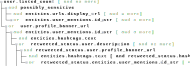
\includegraphics[width=\columnwidth]{SchemaSummarization/img/collapse-FPTree}
\caption{FP-Tree based schema summaries}
\label{fig:summary:fptree}
\end{figure}

\tinysection{FP-Tree Summaries}
An FP-Tree is a trie-like data structure that makes it easier to identify common patterns in a query.  
Every edge in the tree represents the inclusion of one feature, or in our case one attribute.
Hence, every node in the tree corresponds to a set of paths (obtained by traversal from the root), and every leaf corresponds to one source schema.
We observe that every node in an FP tree corresponds to a disjunction: For a node with 3 children, each subtree represents a different branch.  
Similarly, every edge corresponds to a conjunction with a singleton.
Although the resulting tree may duplicate some attributes, duplications are minimized~\cite{DBLP:conf/sigmod/HanPY00}.

\begin{example}
Figure~\ref{fig:summary:fptree} illustrates a schema summary based on  FP-Trees.  
Sequences of nodes with a single child are collapsed into single rows of the display (e.g., \inlinejson{user.listed_count} and 63 immediate descendents).
A toggle switch allows these entities to be displayed to the user, if desired.
Every level of the tree represents a set of alternatives. For example, \inlinejson{possibly_sensitive} never co-occurs with \inlinejson{user.profile_banner_url}.  
\end{example}

\tinysection{RCDC Summaries}
Our second visualization is based on correlations and anticorrelations.
To construct this visualization, we begin with the joint summary.
Recall that the joint summary has the form 
$$(P_1 \vee \emptyset)\;(P_2 \vee \emptyset)\;(P_3 \vee \emptyset)\;(P_4 \vee \emptyset)\ldots$$

We create a covariance matrix based on the probability of two attributes co-occurring in the schemas of one of our input \json records.  
Using this covariance matrix, hierarchical clustering~\cite{Johnson1967}, and a user-controlled threshold on the covariance, we cluster the attributes by parenthesizing.  For example, clustering might group $P_1$ with $P_2$ and likewise $P_3$ with $P_4$.
We can rewrite this formula as:
$$\approx (P_1P_2 \vee \emptyset)\;(P_3P_4 \vee \emptyset)\ldots$$
Observe that this formula omits schemas that the original formula captures (e.g., any schema including $P_1$ but not $P_2$).
However, because clustering ensures that attributes within a group co-occur frequently, there are comparatively few such schemas.

We next repeat the process with a new covariance matrix built using the frequency of co-occurrence of \emph{groups} (like $P_1P_2$).  
As before, we create clusters, but this time we cluster based on extremely negative co-variances.
Hence, members of the resulting clusters are unlikely to co-occur.
Continuing the example, let us assume that $P_1P_2$ and $P_3P_4$ are highly anti-correlated.  
Approximating and simplifying, we get an expression in RCDC form.
$$\approx (P_1P_2 \vee P_3P_4 \vee \emptyset)\ldots$$
As with the FP-Tree display, we use counts and an example attribute as a summary name for the group, and a toggle button to allow users to expand the group along either the OR or AND axes.

\begin{figure}
\centering
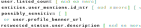
\includegraphics[width=0.8\columnwidth]{SchemaSummarization/img/collapse-RCDC}
\caption{RCDC based schema summaries}
\label{fig:summary:rcdc}
\end{figure}






\section{Visualization}
\label{sec:visualization}
% !TEX root = ../cnf-json.tex

Even within a mostly standardized collection of records like exported Twitter or Yelp data or production system logs, it is possible to find a range of schema usage patterns.
Grouping by [anti-]cooccurrence is one step towards helping users understand these usage patterns, but is insufficient for three reasons:
\begin{enumerate*}
  \item Conceptually distinct fragments of the schema may share attributes in common (e.g., delete tweet records share attributes in common with tweet records).
  \item Even if they do not co-occur, certain [groups of] attributes may be correlated (e.g., due to mobile phones, tweets with photos are also often geotagged).
  \item There is no general way to differentiate \json objects and arrays being used to represent collections from those being used to represent structures (e.g., twitter stores geographical coordinates as a 2-element array).
\end{enumerate*}
The second part of the \systemnametwo interface addresses these issues by presenting top-down visual surveys of the schema.
These surveys help users to quickly assess variations in schema usage across the collection, to identify related schema structures, and to ``drill down'' into finer grained relationships.

%Imagine an analyst is given a mixture of these Twitter \json objects and have two tasks, one where they need to use attributes of user based on tweets, and another where they need to determine 

%\begin{itemize}
%\item user will want to start with one \json schema and want to end with multiple views for different use cases
%\item Problem statement: \json schemas are often 'wide' and contain different sub schemas that map to potential use cases
%\item Through different means we try and recover these use cases and segment the data on these features
%\item then try and prompt the user to generate views until they have all their use cases met
%\end{itemize}

\begin{figure}
  \centering
  \begin{subfigure}{0.4\columnwidth}
    \centering
    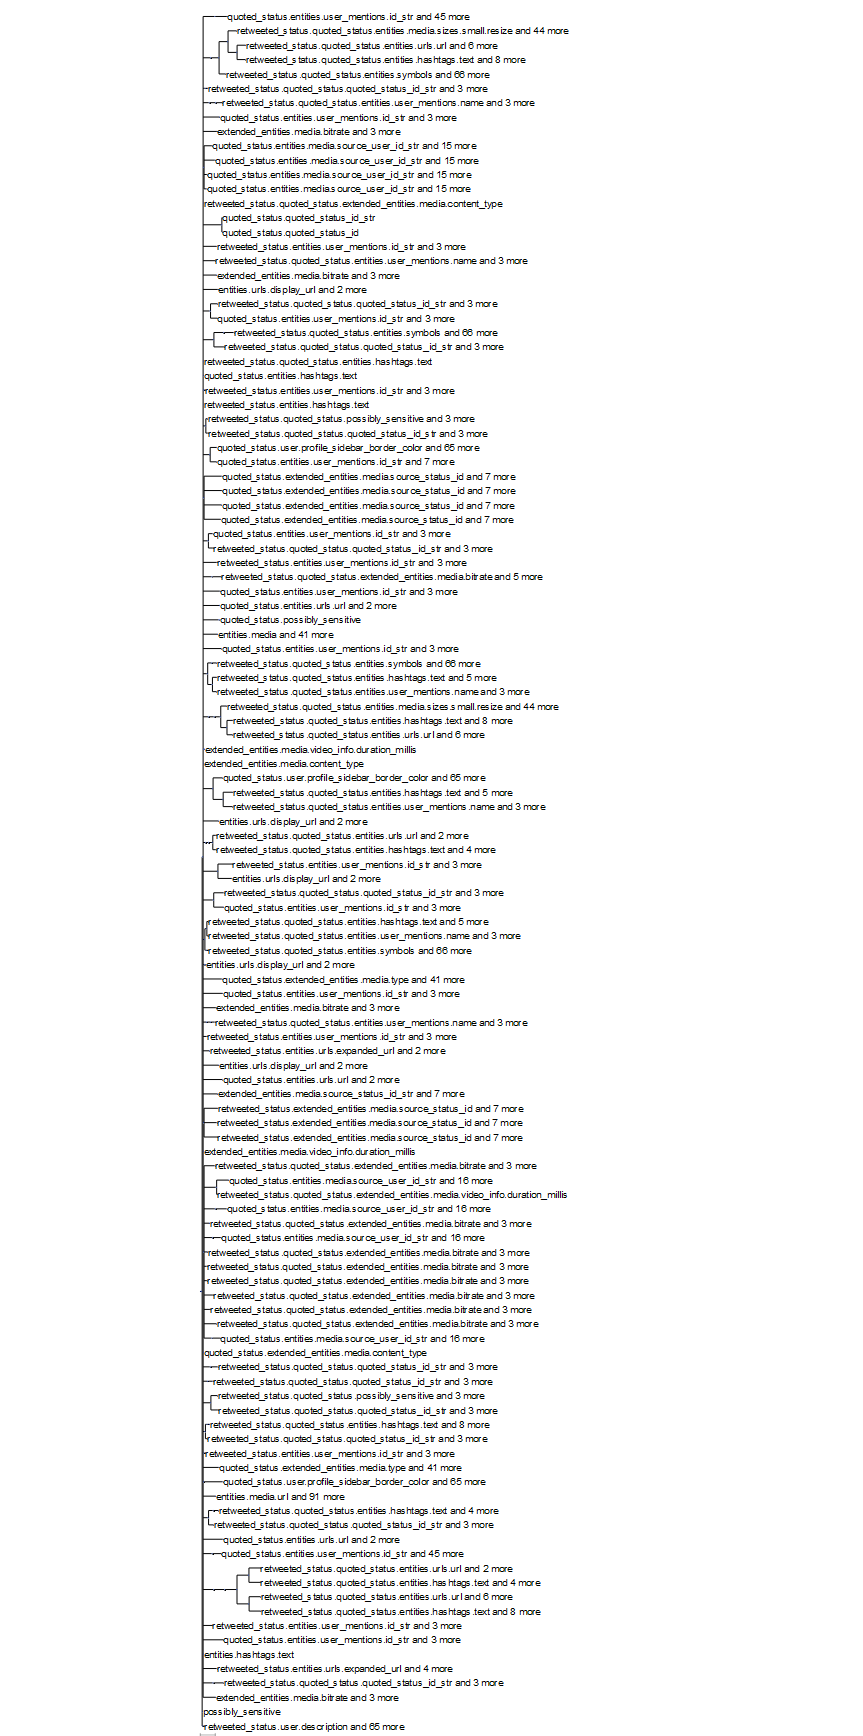
\includegraphics[width=0.57\textwidth]{SchemaSummarization/img/twitterFullTree.png}
    \caption{Without segmentation.}
    \label{fig:seg:twitterFull}
  \end{subfigure}
  \begin{subfigure}{0.59\columnwidth}
    \centering
    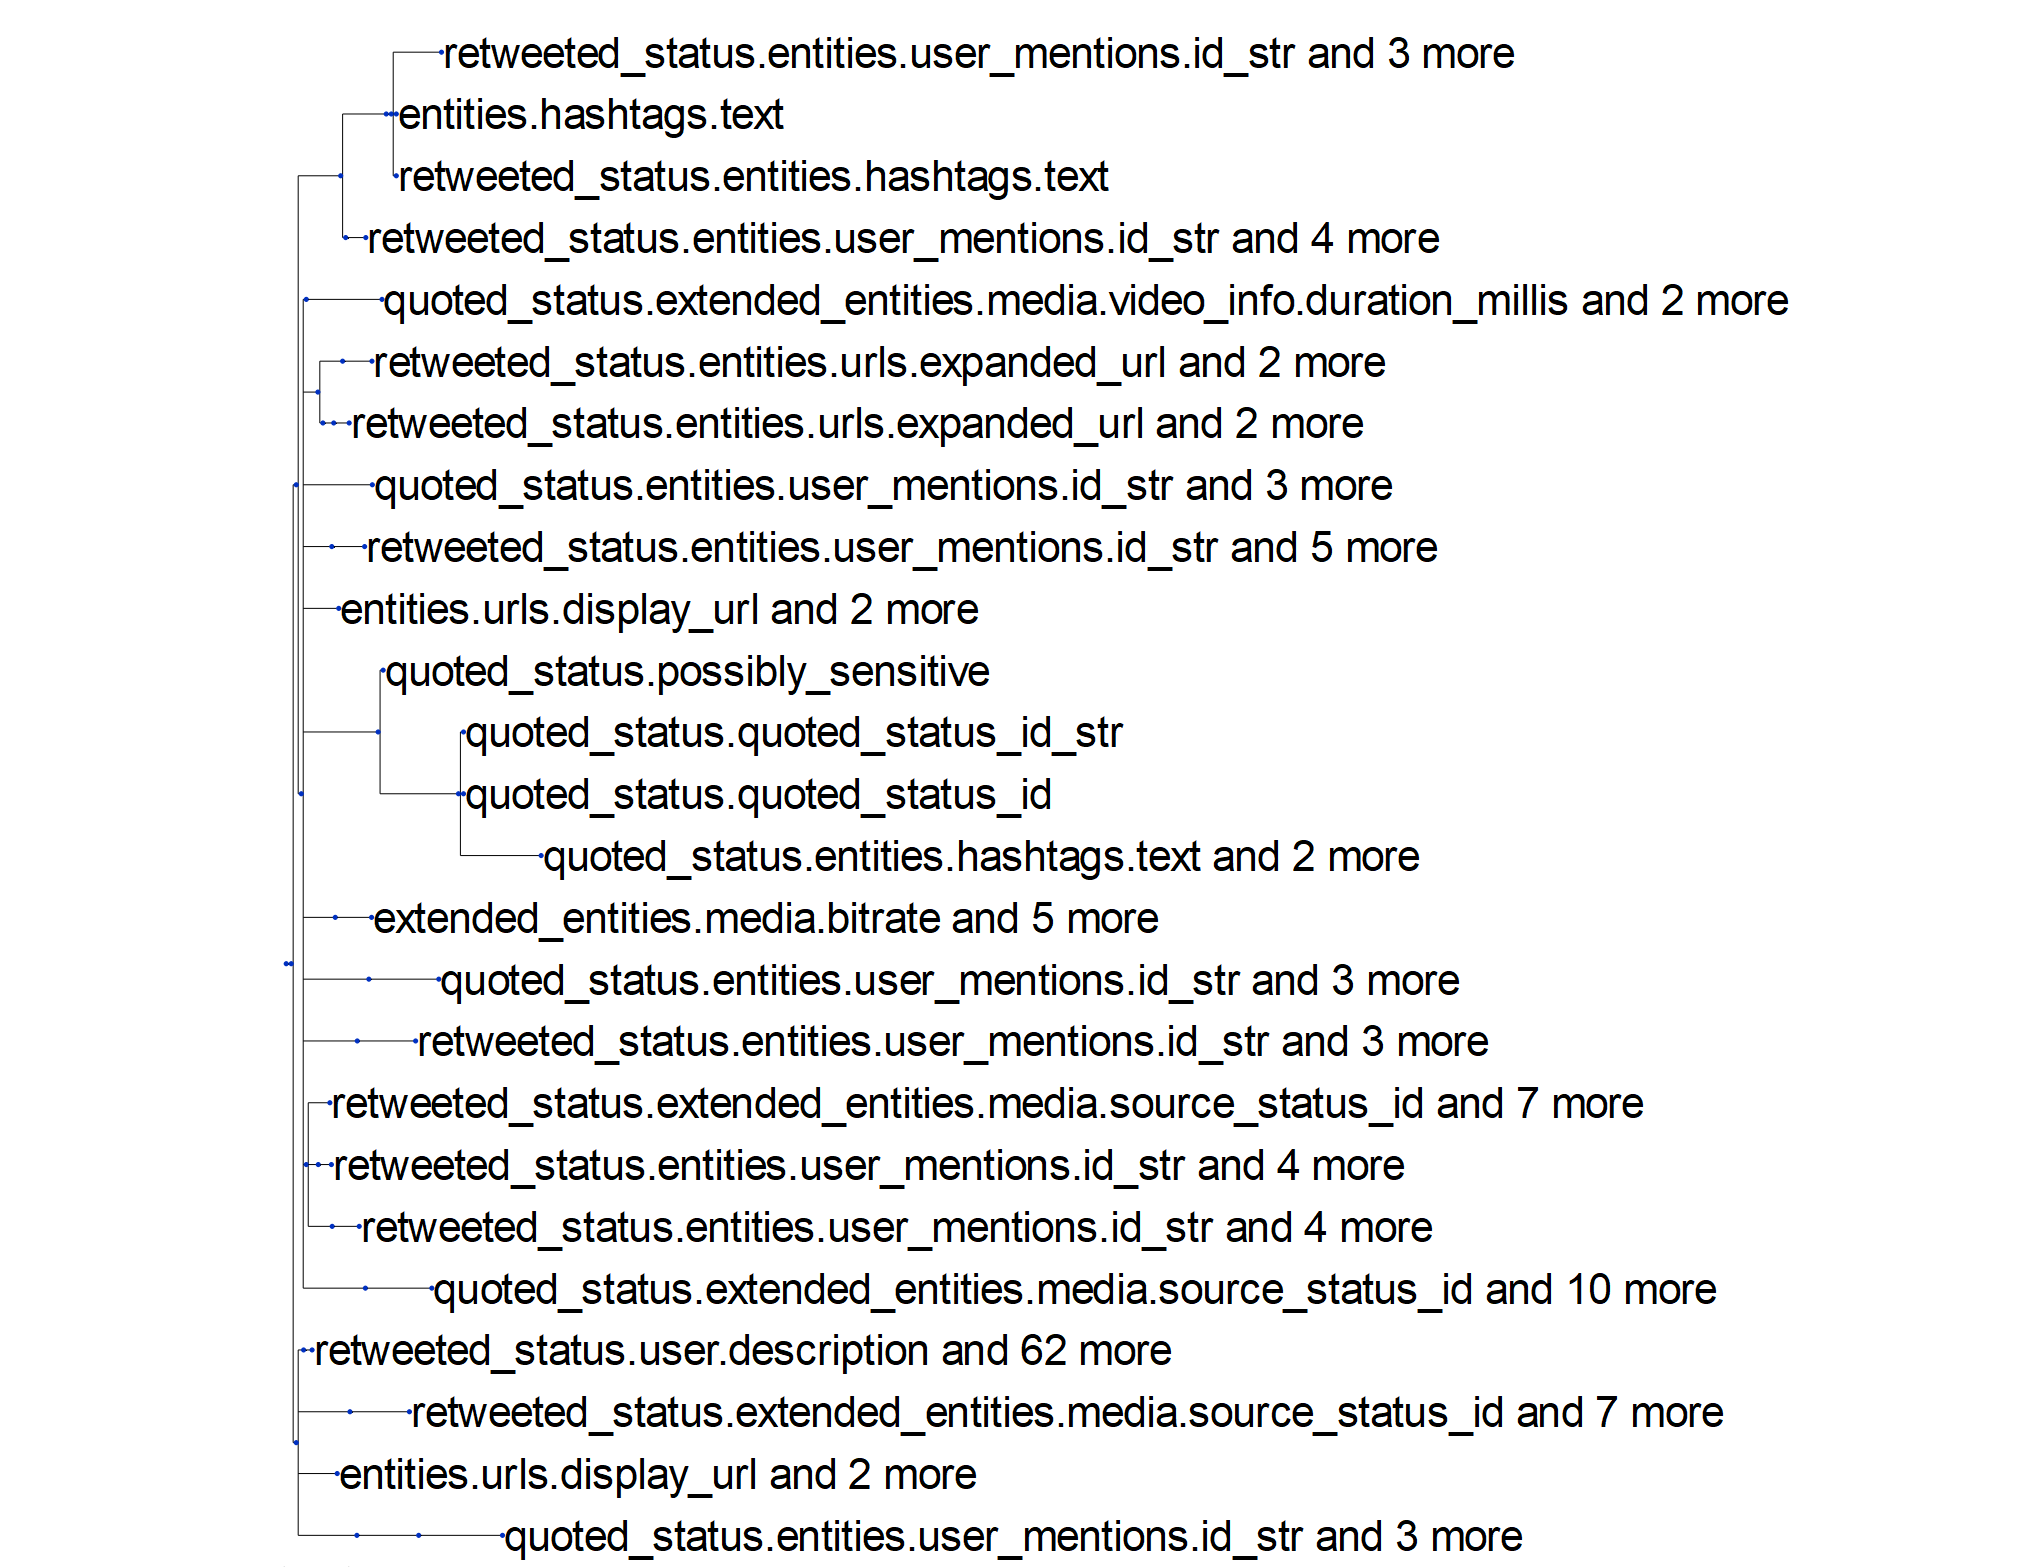
\includegraphics[width=\textwidth]{SchemaSummarization/img/twitterSegment.png}
    \caption{With segmentation.}
    \label{fig:seg:twitterSeg}
  \end{subfigure}
  \caption{Segmentation breaks up schema representations into manageable chunks.}
  \label{fig:seg}
\end{figure}

\subsection{Schema Segmentation}
Specifically, we want to help the user to focus on particular parts of the joint schema;
We want to allow the user to filter out, or segment the schema based on certain required attributes that we call \emph{subschemas}.
We define a subschema $s$ as a set of attributes, where $s$ is contained in one or more source schemas.
Further, the $s$-segment of source schemas $S_1, \ldots, S_N$ to be the subset that contain $s$:
$$\textbf{segment}(s) \defineeq \comprehension{S_i}{i \in [1,N] \wedge s \subseteq S_i}$$
We are specifically interested in visual representations that can help users to identify subschemas of interest.
By then focusing solely on the segments defined by these subschemas can significantly reduce the complexity of the schema design problem, as illustrated in Figure~\ref{fig:seg}.
Figures~\ref{fig:seg:twitterFull} illustrates the full schema summary as a tree, while Figure~\ref{fig:seg:twitterSeg} shows a partial summary identified by the user using the lasso tool we describe shortly.

\begin{figure}[H]
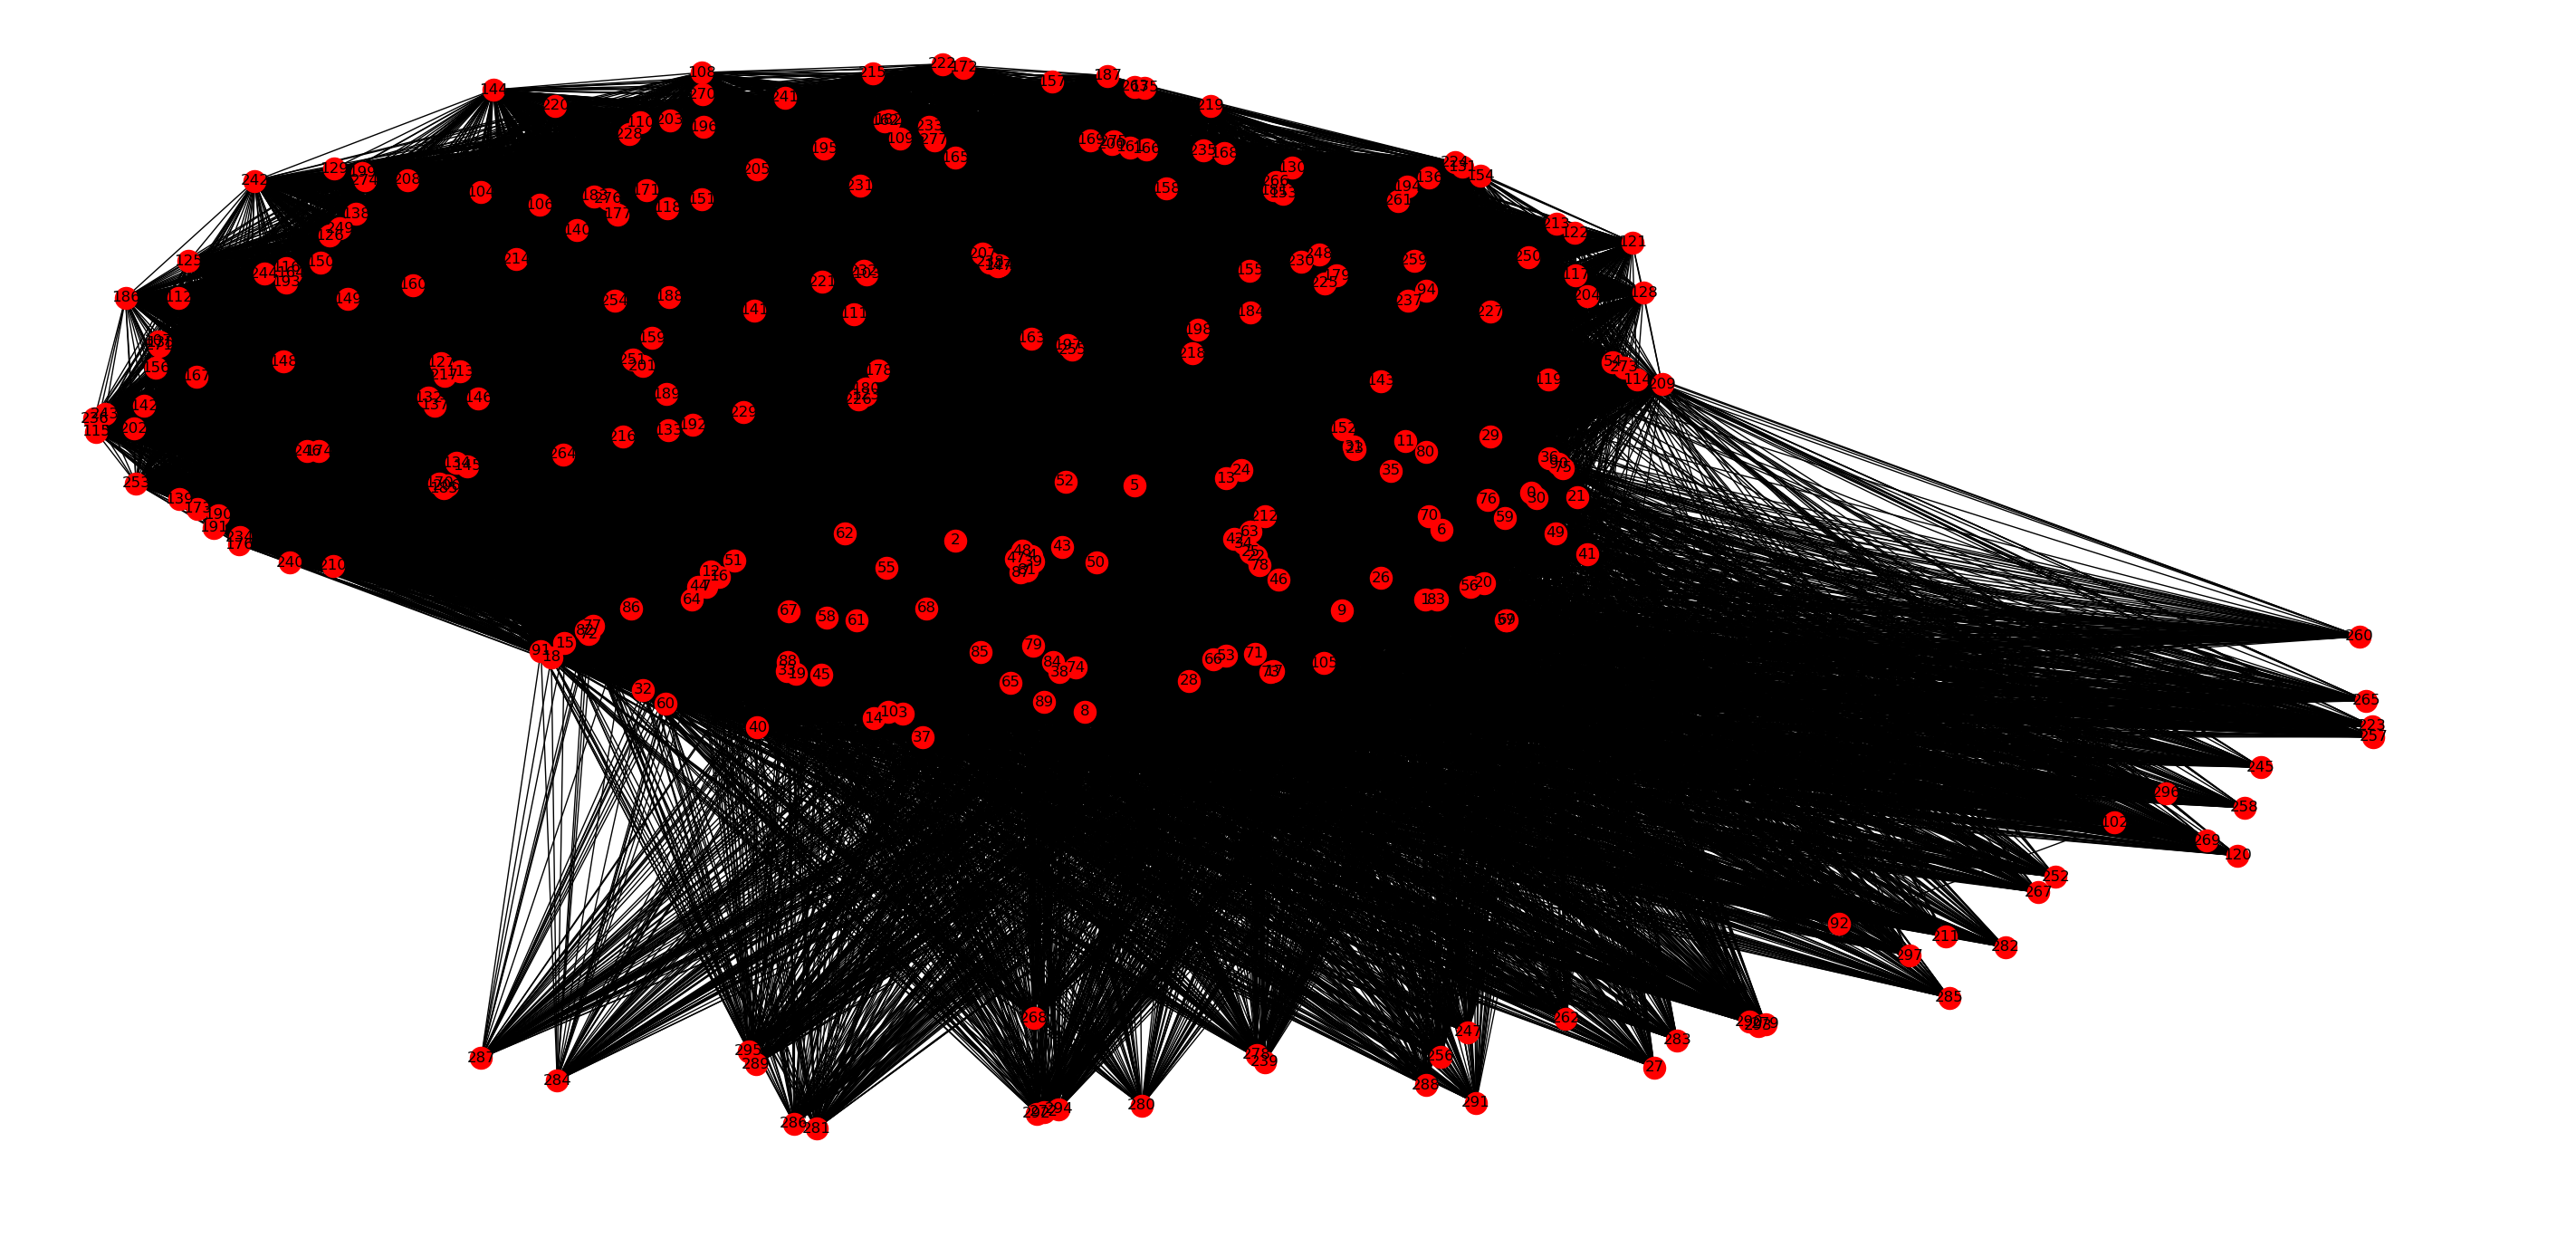
\includegraphics[width=1.0\linewidth]{SchemaSummarization/img/YelpCovMat.png}
\caption{Coveriance Cloud for the full Yelp dataset.}
\label{fig:cloud}
\end{figure}

\tinysection{Covariance Clouds}
Our second visual representation, also like schema summaries, uses correlations and anti-correlations to communicate subschemas of interest.
To generate a covariance cloud, we create a covariance matrix from the source schemas, using the appearance of each attribute as a variable.
Based on a user-controllable threshold, we then construct a graph from the covariance matrix with every attribute as one node, and every covariance exceeding the threshold as an edge.
The graph is then displayed to the user as a cloud using standard force-based layout techniques (e.g., those used by GraphViz~\cite{DBLP:conf/gd/EllsonGKNW00}).  
%\todo{Will: Add figure here}
Cliques in the graph represent commonly co-occurring subschemas that might form segments of interest.  
This includes every conjunctive group identified in the schema summary.
However, unlike the schema summary, this visual representation more effectively captures subschemas with attributes in common.

\tinysection{KNN-PCA Clouds}
While the first visualizaton works on simple schemas, we found that on more complex \json data like Twitter streams~\cite{twitterdecahose}, or the Yelp open dataset~\cite{yelpdata} there were too many inter-attribute relationships, and the resulting visualizatons were noisy.
An approach we settled on is a mixture of Principle Component Analysis (PCA) and K Nearest Neighbor clustering (KNN). 
As before, we treat each source schema as a feature vector with each attribute representing one feature. 
We then use PCA to plot our source schemas in two-dimensions.
The resulting visualization illustrates relationships between source schemas, with greater distances in the visualization representing (approximately) more differences between the schemas.
Hence, clustered groupings of schemas represent potentially interesting sub-schemas.

A key limitation with this visualization is that for more complex datasets the somewhat arbitrary choice of 2 dimensions can be too low.
Conversely adding more dimensions directly through PCA makes the visualization more complicated and hard to follow.
To mitigate these limitations, we use K-Nearest Neighbors (KNN) to colorize the PCA Cloud.
In addition to using PCA, we do KNN clustering on the schemas using a user-provided K (number of clusters).  
Each cluster identified by PCA is assigned a different color.
Combined, these two algorithms to provide users an initial insight into the potential correlations that exist in their dataset.


\begin{figure}
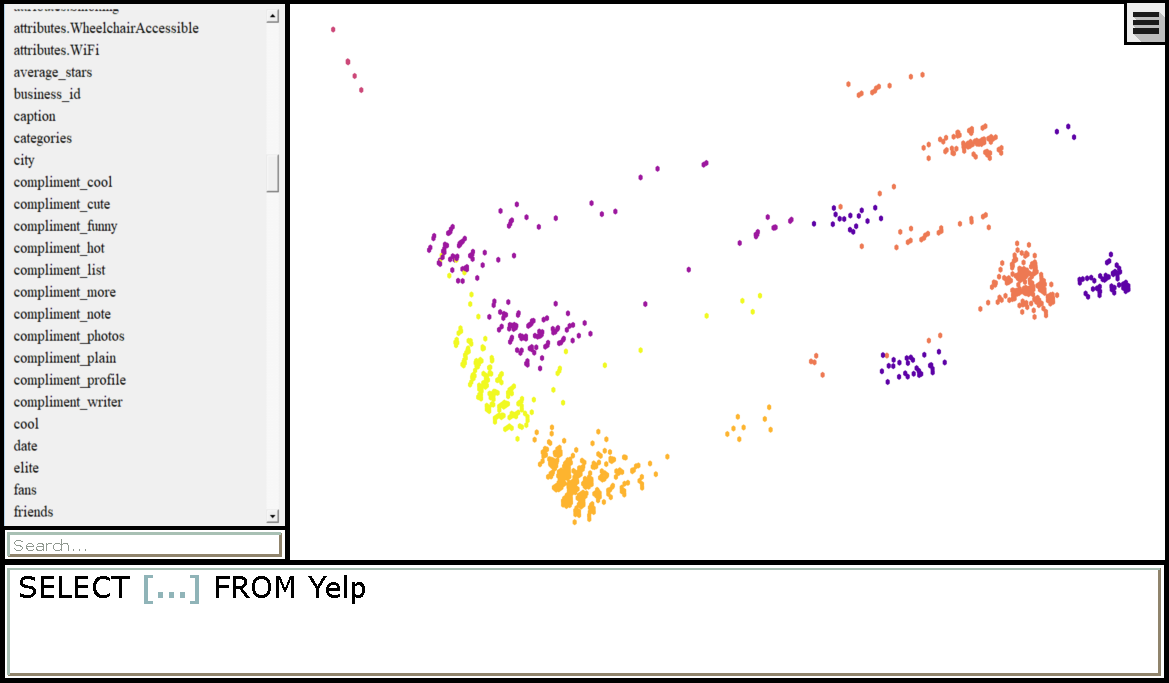
\includegraphics[trim={50mm 25mm 5mm 10mm},clip,width=1.0\linewidth]{SchemaSummarization/img/YelpUI.pdf}
\caption{KNN-PCA cloud with K=6 on the Yelp dataset.}
\label{fig:yelp}
\end{figure}

\begin{example}
Figures~\ref{fig:ui} and \ref{fig:yelp} show an example of the resulting view on Twitter and Yelp data.
Note the much tighter clustering of attributes in the Twitter data: each cluster represents one particular, common type of tweet.
Conversely, the Yelp schema includes a nested collection with, for example, hourly checkins at the business.  
The presence (or absence) of these terminal paths is more variable, and the resulting PCA cloud follows more of a gradient.
\end{example}

These graphs may not initially be intuitive to interpret, but they provide abstract bearings that map directly to phenomenon’s that exist in the data. In lieu of a formal user study, we postulate that the information gained from each algorithm independently will benefit the exploration process that is agnostic to labeled information. This is in contrast to other tools~\cite{Smith:2006:FSS:1187627.1187785}, that largely utilize naming cues and attribute nesting to meet user needs.

\subsection{Schema Exploration}

Now that we have shown the user potentially interesting subschemas, our next task is to help them to (1) narrow down on actually interesting subschemas, and (2) use those schemas to drill down to a segment of the schema data.
For the first step, it is critical that the user develop a good intuition for what the visual representations encode.
One way to accomplish this is to establish a bi-directional mapping between \systemnametwo's two data panes.

To map from visual survey to schema summary, we provide users with a lasso tool.
As illustrated in Figure~\ref{fig:ui}, users can select regions of the KNN-PCA Cloud and the corresponding schemas within that region.  Doing so identifies the maximal subschema contained in all subschemas and regenerates the schema summary pane based only on the segment containing the maximal subschema.  
The maximal subschema itself is also highlighted in the schema summary pane.
On the Covariance cloud, the lasso tool behaves similarly, selecting attributes explicitly rather than a maximal subschema.

The reverse mapping is achieved using highlighting, as illustrated in Figure~\ref{fig:yelpH}.
Users can select one or more attributes (or groupings) in the schema summary pane, and the KNN-PCA Cloud (resp., Covariance Cloud) is modified to highlight schemas in the corresponding segment (resp., to highlight the attributes).
In conjunction with their prior knowledge of their tasks and ideal use cases, we use this approach to perform the initial schema segmentation.

% What patterns immerge and how do we present them
In either case, after selecting a set of attributes or schemas, the analyst may choose to drill down into the selected segment, regenerating both views for the now restricted collection of schemas.
% An analyst may then futher collapse this tree, to produce a view that they can query. Segmentation provides the ability to display tight groups of highly correlated attributes, instead of a large spanning tree that is impossible for a human to process by hand.



% %Attribute co-occurrence can be caused by the presence of an underlying sub-schema and if many co-occur this indicates the presence of a secondary schema, similar to an entity. 
% Segmenting our data first into these entities and then summarizing them, allows us to present the user with features that describe each entity in smaller doses. 
% Additionally, the existence of these entities is derived from insertion methods, and by extension data collection methods, which correspond to natural groupings of attributes that a user expects.


\begin{figure}
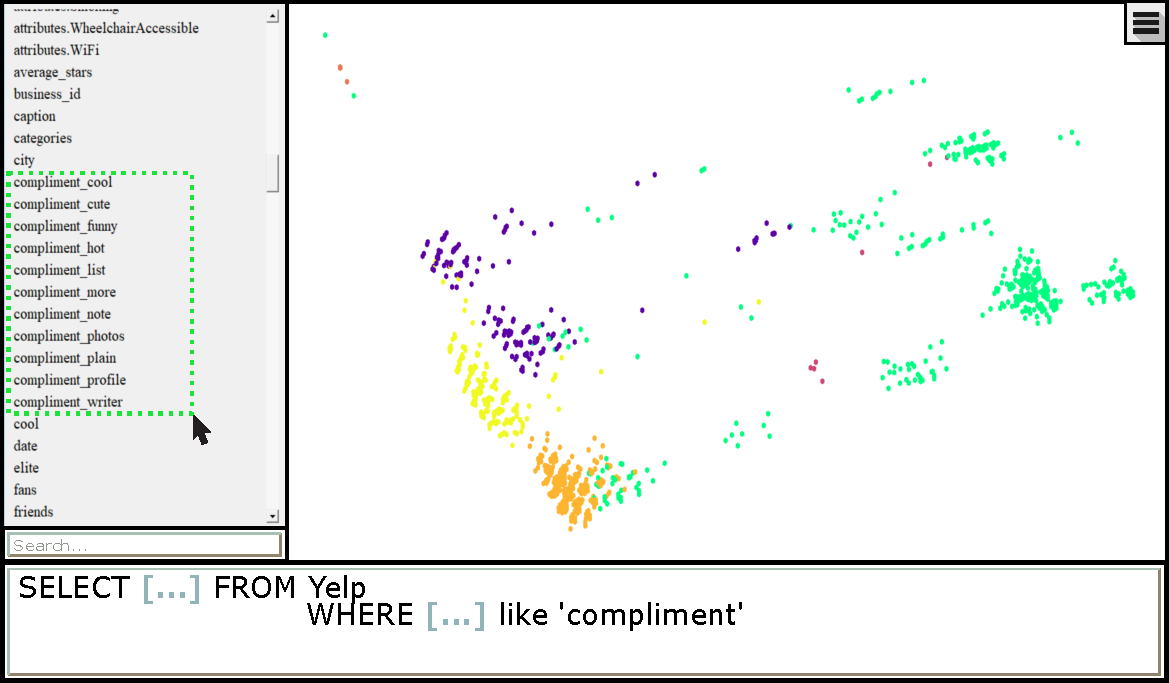
\includegraphics[width=1.0\linewidth]{SchemaSummarization/img/YelpUIH.pdf}
\caption{Points containing user selected attributes are highlighted green.}
\label{fig:yelpH}
\end{figure}


%\begin{itemize}
%\item cov matrix clique issues
%\item knn limitations
%\item PCA limitations and benefits
%\item goal is to first reduce the 
%\end{itemize}

%Through our user interface groups of attributes may be highlighted, this then feeds back into our PCA plot to highlight the points that these attributes are present in. 
%If this group of attributes has high co-occurrence, then they are likely to appear grouped and ideally leads the user to other attributes that also co-occur and are of significance.

\subsection{An Iterative Approach}
At any time in our exploration pipeline analysts may stop where they are, take the knowledge they gained about their dataset, and restart the process from the beginning. 
Through exploring the Twitter dataset we found retweets and quoted tweets to have a high correlation, with this knowledge we can then start back at the beginning and depending on whether our task allows us to merge these attributes, we can then choose a more appropriate K value for KNN. 
In addition, attributes that have no relationship to core attributes, such as a users profile\_image\_url being present, can easily be pruned to compress our summary output. 
By incrementally learning about their dataset, an analyst can converge on the views required for their tasks.


%Will: How does the data get summarized for user consumption. 
%Some UI sketches/screenshots would be appropriate.
%\begin{itemize}
%\item The schema is presented to the user
%\item The user is then shown a 2-dimensional representation of their data using PCA
%\item Iteratively use a generic clustering algorithm to help detect clusters and relationships in their data
%\item Select a subregion of the map to expore relaitonships that exist and what each group represents
%\item |eigenVector| x norm($\sum\nolimits $multiplicity x featureVector), this results in a score for each column that is based on occurance and variation
%\item the higher this score, the more 'representative' of the cluster this feature is
%\item Iterate through this process to determine what the defining characteristics of each group is, and how it relates to other groups
%\end{itemize}




% \section{Iteration}
% \label{sec:iteration}
% 

What facilities do users have for probing for more information, refining the current view, and/or marking the current view as sufficient.

% \section{Experiments}
% \label{sec:experiments}
% 

Time and space permitting...

\section{Related Work}
\label{sec:related}
% -*- root: ../cnf-json.tex -*-
 \tinysection{Schema Extraction}
Schema extraction for \json, as well as for other self-describing data models like XML has seen active interest from a number of sources. 
An early effort to summarize self-describing \emph{hierarchical} data can be found in the LORE system's DataGuides~\cite{DBLP:conf/vldb/GoldmanW97}.
DataGuides view schemas begin with a forest of tree-shaped schemas and progressively merge schemas, deriving a compact encoding of the forest as a DAG.
Although initially designed for XML data, similar ideas have been more recently applied for \json data as well~\cite{DBLP:conf/cidr/LiuG15,DBLP:conf/sigmod/LiuHMLC16}.
Key challenges in this space involve simply extracting schemas from large, multi-terabyte collections of \json data~\cite{DBLP:conf/edbt/BaaziziLCGS17}, as well as managing ambiguity in the set of possible factorizations of a schema~\cite{DBLP:conf/dbpl/BaaziziCGS17,spoth:2017:cidr:adaptive}.
The approach taken by Baazizi et. al.~\cite{DBLP:conf/edbt/BaaziziLCGS17} in particular adopts a type unification model similar to ours, but lacks the conjunctive operator of our type-system.
For non-hierarchical data, interactive tools like Wrangler~\cite{DBLP:conf/chi/KandelPHH11} provide an interactive frameworks for regularizing schemas.

\tinysection{Physical Layout}
While schemas play a role in the interpretability of a \json data set, they can also help improve the performance of \json queries.  
One approach relies on inverted indexes~\cite{DBLP:conf/cidr/LiuG15} to quickly identify records that make use of sparse paths in the schema.
Another approach is to normalize schema elements~\cite{DBLP:conf/sigmod/DiScalaA16}.  Although the resulting schema may not always be interpretable, this approach can result in substantial space savings.

\tinysection{Information Retrieval}
From a more general perspective, the schema extraction problem which aims at making large datasets tractable for interactive exploration, is an instance of \textit{categorization} problem that has been repeatedly studied in the literature.
More precisely, attributes (metadata) of the datasets can be grouped into a hierarchy of "facets" (i.e., categories)~\cite{Smith:2006:FSS:1187627.1187785} where the child-level facets are conditioned on the presence of the parent one.
In our approach, we adopt the hierachical data visualization and focus more on the algorithmic essence of the problem: How to (1) balance between the preciseness and conciseness of the visualization and (2) respond to users' data exploration requests in a scalable way.

\section{Future Work}
\label{sec:future}
% !TEX root = ../cnf-json.tex
One challenge that we will need to address in \systemnametwo is coping with nested collections.  
At the moment, the user can manually merge collections of attributes that correspond to disjoint entites.
However, we would like to automate this process.
One observation is that a typical collection like an array has a schema with the general structure:
$$(P_1 \vee P_1P_2 \vee P_1P_2P_3 \vee \ldots)\;=\;(P_1 \wedge (\emptyset \vee P_2 \wedge (\emptyset \vee P_3 \wedge (\ldots)) ))$$
The version of this expression on the right hand side is notable as its closure over the semiring $\tuple{\big\{\{\mathbf P\}\big\}, \vee, \wedge, \emptyset, \big\{\{\}\big\}}$ would indicate that the semiring is ``quasiregular'' or ``closed'', an algebraic structure best associated with the Kleene star.
Hence, we plan to explore the use of the Kleene star to encode nested collections in our algebra.
A key challenge in doing so is detecting opportunities for incorporating it into a summary, a more challenging form of the factorization problem.

A further step to increase the capabilities of \systemnametwo is to incorporate type information in the summarization. 
This adds an extra layer of information an analyst can extract from our system, as well as the ability to identify and correct schema errors. 
As a long term goal we will provide capabilities for linking views, for example by defining functional dependencies.
The goal is to create full entity relationship diagrams. 
In particular, one interesting way to identify potential relationships that exist between entities is by leveraging the overlap between segments.

\chapter{Application: Summarizing Probabilistic Databases}
\label{chapter:summarizeprobabilisticdatabases}

\section{Introduction}
% !TEX root = ../paper.tex
Many tasks in machine learning, information extraction, etc, generate uncertain data.
That is, output tuples generated from one probabilistic prediction differ from the other.
Though it is a general practice to deterministically output the most probable prediction, it is beneficial to explore other possible predictions, especially when an application needs to compare predictions under different parameter tuning strategies~\cite{papadakis2016comparative}.
However, as~\cite{Gupta:2006:CPD:1182635.1164210} pointed out, state-of-the-art statistical models of information extraction provide a sound probability distribution over extractions but are challenging to represent and query in relational framework.

One naive strategy would be letting the application to iterate over all observed outputs, together with their probabilities of being observed.
This strategy, on one extreme, defines a \emph{probabilistic database}~\cite{suciu2009probabilistic} and walks the application through the \emph{entire space} of possible worlds.
This is a sufficient condition for the application to discover all information that may be useful: the probability that any set of tuples will be contained in the output.
However, this naive strategy puts an unnecessary burden on the application side.
That is, there are practically exponential number of possible outputs~\cite{Gupta:2006:CPD:1182635.1164210}.  
Each observed output may contain duplicate tuples and it is possible to deliver the probability distribution over possible outputs in a more compact way.

The other naive strategy would be letting the application view each \emph{individual} tuple together with the probability that the tuple is contained in an output.
The probability of any \emph{set} of tuples can then be estimated by multiplying the probability of each content tuple. 
This strategy, on the other extreme, defines a \emph{tuple-independent probabilistic database}~\cite{suciu2009probabilistic} that compactly represents the distribution of outputs by assuming each tuple independently exists in an output.
However, for applications where tuples are predominantly correlated in the output, probabilities delivered by tuple-independent probabilistic database may greatly deviate from the truth~\cite{Gupta:2006:CPD:1182635.1164210}.
Consider an example application where tuple-correlation is dominant by nature.
\begin{example}
Consider an \emph{Enitity Resolution (ER)} task where the input is a set of tuples where each tuple contains a set of attributes that may help to determine whether two tuples are different facets of the same entity.
The output will be the same set of tuples but augmented with an additional attribute indicating its predicted entity ID.
\end{example}
Since the prediction is uncertain, the output data can be viewed as a space of possible sets of augmented tuples that a predictor may generate.
Augmented tuples in the output are correlated by design, that is, given that a tuple $\tuplesymbol$ is assigned entity ID $eid$, other tuples having attributes similar to $\tuplesymbol$ being assigned the same $eid$ increases and are no longer independent events.
This example can be generalized to classification or clustering related tasks where the output is a set of label-augmented tuples where the label assignments are uncertain.

To encode tuple correlation, various kind of auxiliary information  (e.g., \emph{c-tables}~\cite{suciu2009probabilistic}, factors~\cite{friedman1999learning,sen2007representing, sen2009prdb}, Markov Logic~\cite{jha2012probabilistic}) are introduced for delivering more accurate probabilities. 
Auxiliary information inevitably increases the model complexity, making the inference of the desired probabilities harder.
It also puts a heavier burden on the application side for digesting the representation.

To carefully introduce auxiliary information, we start by considering \emph{c-tables}~\cite{suciu2009probabilistic}.
A c-tables compactly represents the distribution over outputs by presenting only individual tuples, annotated with a propositional formula.
A tuple exists in the output iff its propositional formula evaluates to be true.
By walking the application through a c-table as well as the corresponding probability distribution over variables in its formula, we equivalently delivers the distribution of possible outputs.
However, linking the probability distribution with its c-table generally requires heavy weight inference.
That is, to compute the probability of a set of tuples being co-existent, we need to enumerate all possible evaluations of their variables such that their propositional formula are true.
This process is non-trivial especially when we need to repeated compute such probabilities for different sets of tuples.
Moreover, in our example application, it is generally difficult to obtain such propositional formula, since tuple correlation is caused by the complex nature of some predictor.
As a result, for our target applications, we only expect a tuple in the c-table to be annotated with a single distinct variable $X_i$ with $X_i=1$ meaning the presence of the $i$th tuple in the output.
The probability of two tuples $\tuplesymbol_i,\tuplesymbol_j$ being co-existent is directly linked with the marginal probability $p(X_i=1,X_j=1)$.
To deliver the distribution of outputs, we need to walk an application through the c-table and the joint distribution $\possibleworldsdistribution=p(\ldots,X_i,\ldots)$.
Enumerating all valuations of the variables is not practical.
Instead, we group correlated variables together and only enumerate valuation within each group.
This essentially creates a \emph{factor} for each group. 
Mappings in a factor is still exponential with respect to the number of correlated variables.
In this paper, we study the problem of encoding the joint distribution $\possibleworldsdistribution$ by only a subset of mappings in factors.
We show how desired probabilities of the distribution $\possibleworldsdistribution$ can be computed by the lossy encoding. 
Due to incomplete mappings, the computed probabilities generally deviates from the truth.
However, the encoding allows finer granularity in trading-off between conciseness and probability computation accuracy.
That is, by gradually populating the mappings in a factor, an application can choose to obtain an encoding that incurs a high-fidelity in computing probabilities but is verbose, or obtain a more compact encoding that incurs a greater loss of accuracy. 
To manage the loss-rate, we develop a framework for reasoning about the trade-off between verbosity and fidelity.   
While the encoding does not admit closed-form solutions to classical information theoretical fidelity measures like information loss, we propose an efficiently computable fidelity measure called \Errorname.  

\tinysection{Contributions}

\tinysection{Roadmap}




\section{Problem Definition}
% !TEX root = ../paper.tex
\tinysection{Input Definition}
As shown in Figure~\ref{fig:systemoverview}, the input data consists of a finite set of possible instances $\instances=\{\instance_1,\ldots,\instance_n\}$ where each instance $\instance_i$ consists of a set of tuples.
We use the \emph{possible worlds semantics}~\cite{Dalvi:2009:PDD:1538788.1538810} and call $\instances$ as \emph{possible worlds}.
Each world is assigned a probability by the distribution $\possibleworldsdistribution : \instances \to [0,1]$ such that $\sum_i \possibleworldsdistribution(\instance_i) = 1$.
In other words, our input is defined as a discrete probability space $\probabilisticdatabase=(\instances,\possibleworldsdistribution)$.

\tinysection{Goal}
An application theoretically may require scanning through all possible worlds, in order to aggregate the probabilities where the corresponding worlds contain some target \emph{set} of tuples.
In the context of Entity Resolution task, an application may require aggregating probabilities of all predictions that contain tuples labeled by a target $eid$. 
For convenience, we will refer to these aggregated probabilities as \emph{marginal probabilities} or simply \emph{marginals} in the rest of the paper.
Our goal is then to help the application efficiently explore and compute marginals in a practical way without iterating through a large number of possible worlds.

\tinysection{System Overview}
We begin by giving the reader an overview on how the input flows \emph{theoretically} and \emph{practically} to a client-side application.
In Figure~\ref{fig:systemoverview}, the red dashed lines encompasses a theoretical data flow that iterates through all possible worlds.
In practice, possible worlds in the input will converted into an initial form of representation.
Based on the initial form, further compression can be made that provides a materialized view over the input.
The materialized view can be efficiently queried and the query result will be simplified before being presented to the application.

\begin{figure*}[ht!]
    \centering 
     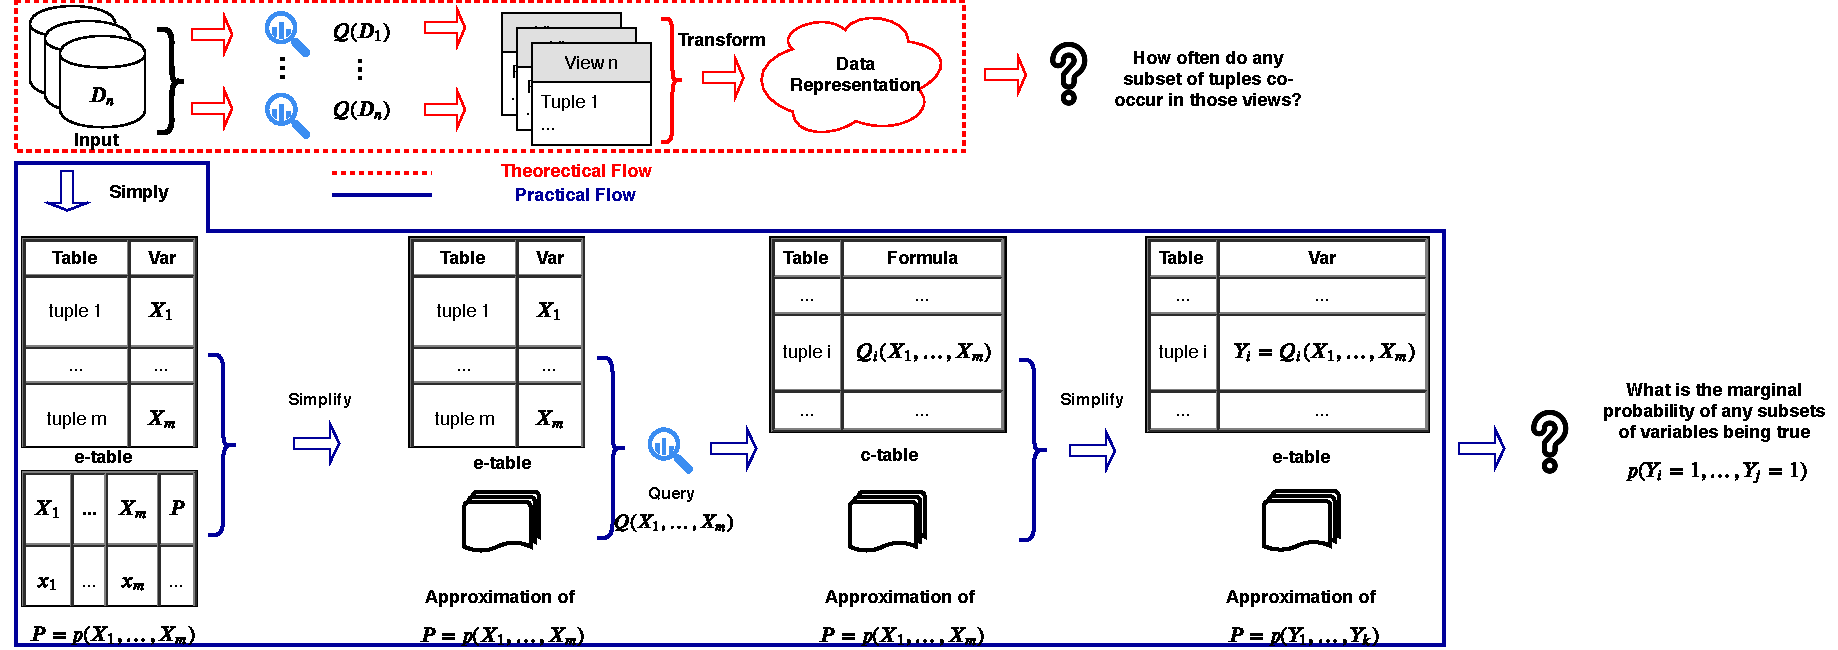
\includegraphics[width=\textwidth]{ProbabilisticDatabaseSummarization/graphics/Data_Flow_Diagram.pdf}
     
 \bfcaption{Theoretical v.s. Practical Data-flows.}
 \label{fig:systemoverview} 
 \trimfigurewhitespace
\end{figure*} 

\subsection{Practical Input Representation}
\label{sec:outputrepresentation}
The previous definition of $\instances$ does not suggest a practical representation, especially when explicit enumeration of all possible worlds is not feasible when $n$ is very large.

\tinysection{C-tables and pc-tables}
We adopt \emph{c-tables} to compactly represent $\instances$. 
A \emph{c-table}~\cite{suciu2009probabilistic} is a set of \emph{distinct} tuples contained in all possible worlds, with each tuple annotated by a propositional formula over random variables.
A \emph{valuation} over these variables assigns each propositional formula a truth value, indicating the existence of the corresponding tuple in a world.
There is a many-to-one mapping from valuations to a possible world.
Extending a c-table by a joint probability distribution over random variables, the resulting \emph{pc-table} can represent any probabilistic database $\probabilisticdatabase$~\cite{suciu2009probabilistic}.

\tinysection{Simplified C-tables}
For our example application, there are two limitations by adopting a general c-table representation.
Firstly, it is difficult to obtain such propositional formula due to lack of knowledge on how tuples are correlated in $\probabilisticdatabase$.
That is, due to complex nature of the function that generates $\probabilisticdatabase$, it is generally hard to formulate how tuples are correlated.
Secondly, the mapping from valuations of variables to possible worlds is many-to-one for a general c-table.
To compute desired marginals, it may require an expensive aggregate over all valuations that map to the same world. 

To overcome the limitations, we represent our input by a family of simplified c-tables, which we call \emph{existence tables} or simply \emph{e-tables}.
Each tuple $\tuplesymbol_i$ in an e-table is annotated with a single random variable $X_i$ whose value is $1$, meaning that the $i$th tuple exists in a world, or $0$ otherwise.
We refer to these variables as \emph{existence variables}.
There is an \emph{one-to-one} mapping from a valuation of existence variables $(x_1,\ldots,x_n)\in\{0,1\}^n$ to a world $\instance$.
The probability of the world (i.e., $\possibleworldsdistribution(\instance)$) can be computed directly from the joint probability distribution $p(X_1=x_1,\ldots,X_n=x_n)$.
When it is clear from context, we abuse notation and denote the distribution $p(X_1=x_1,\ldots,X_n=x_n)$ also as $\possibleworldsdistribution$.
We call an e-table, together with $\possibleworldsdistribution$, a \emph{pe-table}. 

\subsection{Summarizing Joint Distribution}
It is not practical, both in space and marginal computation efficiency, to present pe-table in a view that iterates through all valuations (i.e., worlds) of existence variables.
Hence we need a view that summarizes $\possibleworldsdistribution$ into a more compact form.

\tinysection{Naive Summary}
There can be a set of tuples $\{\ldots,\vec t_i,\ldots\}$ independent of each other such that, 
$$p(\ldots,X_i=1,\ldots)=\Pi_i\;p(X_i=1)$$
In other words, we do not need to store valuations of any combination of those variables in the view, which greatly reduces the number of parameters.
We name the set of parameters $p(X_i=1)$ as a \emph{naive summary} and return to it through out the rest of this paper.
The naive summary is often referred to as \emph{tuple-independent} model~\cite{suciu2009probabilistic}.
When variables are correlated, which is prevalent in our example application, the marginals computed from a naive summary are error-prone.

\tinysection{Loss-less Summary}
For tuples whose variables that are correlated, a \emph{factor graph}~\cite{friedman1999learning} that is equivalent to the marginal probability distribution over these variables, is a sufficient condition for computing any relevant marginals. 
However, it requires heavy weight inference to obtain such set of factors and for each factor, the number of parameters is still exponential to the number of variables that the factor contains.

\tinysection{Lossy Summary}
Practically an application may not require computing exact marginals for \emph{every} set of tuples and we can \emph{cache} marginals that are frequently computed and offer estimation on others. 
Specifically, in our example Entity Resolution task, an application may require to explore labelled tuples that are contained in \emph{all} possible predictions, and tuples that are (in-)frequently or otherwise statistically significant.
The application may tolerate inexact marginal computation for other sets of tuples. 
This observation motivates us to study the option of a \emph{lossy} summary containing only a limited number of marginals and offers estimation on marginals not contained.

\subsection{Pattern-based Summary}

\tinysection{Patterns}
We name a set of co-existing tuples as a \emph{pattern}.
More formally we define a \emph{pattern} as an arbitrary binary vector $\pattern=(x_1,\ldots,x_n)$ with $x_i=1$ meaning the $i$th tuple being present in the pattern.
A pattern $\pattern$ is \emph{contained} in the other $\bar{\pattern}$ if $\forall i, x_i\leq \bar{x}_i$, denoted as $\pattern \subseteq \bar{\pattern}$.
Note that a world $\instance$ is a pattern by definition.
Randomly drawing a world $\instance\in\instances$ from $\probabilisticdatabase$, the probability that it contains pattern $\pattern$ is defined by:
\begin{equation*}
  p(\instances \supseteq \pattern) = \sum_i\possibleworldsdistribution(I_i)\mathbf{1}_{\pattern}(I_i) \;\text{where}\;  \mathbf{1}_{\pattern}(I_i)  =
    \begin{cases}
      1 & \text{if $I_i \supseteq \pattern$}\\
      0 & \text{otherwise}\\
    \end{cases}       
\end{equation*}
In pe-tables, $\marginal$ is equivalent to marginal probability $p(X_1\geq x_1,\ldots,X_n\geq x_n)$.
We call $\marginal$ as the \emph{marginal} of a pattern.

\tinysection{Pattern-based Summary}
Denote the mapping $\encoding_{max}$ from each pattern $\pattern$ to its marginal:
$$\encoding_{max} = \comprehension{\pattern \rightarrow \marginal}{\pattern \in \{0,1\}^n}$$
A \emph{pattern-based summary} $\encoding$ is any such partial mapping $\encoding \subseteq \encoding_{max}$. 
We denote the marginal of pattern $\pattern$ in summary $\encoding$ by $\encoding[\pattern] $ ($= \marginal$).
When it is clear from context, we abuse syntax and also use $\encoding$ to denote the set of patterns it maps (i.e., $domain(\encoding)$).
Hence, $|\encoding|$ is the number of mapped patterns, which we call the summary's \emph{verbosity}.




\section{Marginal Estimation}
A pattern-based summary not only delivers marginals that it contains, but also helps in estimating those that are not explicitly given.

\tinysection{Naive Summary Revisited}
Before detailed explanation, we first consider an intuitive example.
There is one specific family of pattern-based summaries that treat each tuple as being independent, which is equivalent to naive summaries discuss in Section~\ref{sec:outputrepresentation}.
As a re-phrase, we call a pattern-based summary as a naive summary $\naiveencoding$ if it is composed of all patterns that have exactly one possible tuple $\tuplesymbol_i$ with marginal $p(X_i\geq 1)$:
$$domain(\naiveencoding)=\comprehension{(0, \ldots, 0, x_i, 0, \ldots, 0)}{i \in [1,n],\; x_i = 1}$$
To estimate marginals not given in the summary, we apply multiplication $$p(X_1\geq x_1,\ldots,X_n\geq x_n)=\Pi_{i=1,n}\, p(X_i\geq x_i)$$

\tinysection{Patterns as Constraints}
For an arbitrary summary $\encoding$, we characterize its process of marginal computation by defining a \emph{space} (denoted by $\Omega_\encoding$) of distributions $\rho \in \Omega_\encoding$ allowed by a summary $\encoding$.
This space is defined by constraints as follows:
First, we have the general properties of probability distributions:
\begin{center}
$\forall \, \instance_i\in \{0,1\}^n : \rho(\instance_i)\geq 0$
\hspace{10mm}
$\sum_{i=1,2^n}\rho(\instance_i)=1$
\end{center}
Each pattern $\pattern$ in the summary $\encoding$ constrains relevant probabilities in distribution $\rho$ to sum to the target marginal:
\begin{equation*}
\forall \pattern \in domain(\encoding)  :\;\; \encoding[\pattern] = \sum\nolimits_{\instance\supseteq\pattern} \rho(\instance) \;\;\;
\end{equation*}
The dual constraints $1-\encoding[\pattern]=\sum_{\instance\not\supseteq\pattern} \rho(\instance)$ are redundant under the constraint $\sum_i\rho(\instance_i)=1$.

The resulting space $\Omega_\encoding$ is the set of all permitted distributions, or equivalently all input $\probabilisticdatabase$, that obey these constraints.
As a result, the distribution $\rho\in\Omega_\encoding$ that the summary delivers is ambiguous: We model this ambiguity using a random variable $\mathcal P_\encoding$ with support $\Omega_\encoding$.
The true distribution $\possibleworldsdistribution$ must appear in $\Omega_\encoding$, denoted as $\possibleworldsdistribution\equiv\truedistribution\in\Omega_\encoding$ (i.e., $p(\mathcal P_\encoding = \truedistribution) > 0$). 
Of the remaining distributions $\rho$ admitted by $\Omega_\encoding$, it is possible that some are more likely than others.
This prior knowledge may be modeled as a prior on the distribution of $\mathcal P_\encoding$ or equivalently by an additional constraint.
However, for the purposes of this paper, we take the uninformed prior by assuming that $\mathcal P_\encoding$ is uniformly distributed over $\Omega_\encoding$:
\begin{equation*}
\label{uniformprior}
p(\mathcal P_\encoding = \rho) = 
\begin{cases}
\frac{1}{|\Omega_\encoding|} & \text{if } \rho \in \Omega_\encoding\\
0 & \text{otherwise}
\end{cases}
\end{equation*}

The summary delivers marginals by randomly picking one permitted distribution from the entire space and aggregate probabilities accordingly.


\section{Summary Accuracy}
% !TEX root = ../paper.tex
The accuracy of such delivery can be considered from two related, but subtly distinct perspectives:
(1) \emph{Ambiguity} measures how much room the summary leaves for interpretation and 
(2) \emph{Deviation} measures how reliably the summary approximates the target distribution $\truedistribution$.

\smallskip
\tinysection{Ambiguity}
We define the Ambiguity $\ambiguity(\encoding)$ of a summary as the entropy of the random variable $\mathcal P_\encoding$. 
The higher the entropy, the less precisely $\encoding$ identifies a specific distribution.
$$\ambiguity(\encoding) = \mysuml_{\rho}p(\mathcal P_\encoding = \rho)\log \left(p(\mathcal P_\encoding=\rho)\right)$$

\tinysection{Deviation}
The deviation from any permitted distribution $\rho$ to the true distribution $\rho^*$ can be measured by the Kullback-Leibler (K-L) divergence $\mathcal{D}_{KL}(\rho^*||\rho)$.
We define the Deviation $\deviation(\encoding)$ of a summary as the expectation of the K-L divergence over all permitted $\rho \in \Omega_\encoding$:
$$\deviation(\encoding)=\expect_{\mathcal{P}_\encoding}\left[\mathcal{D}_{KL}(\rho^*||\mathcal{P}_\encoding)\right] = \sum_{\rho \in \Omega_\encoding} p(\mathcal P_\encoding = \rho) \cdot \mathcal{D}_{KL}(\rho^*||\rho)$$

\tinysection{Limitations}
Neither Deviation nor Ambiguity has a closed-form formula and it is not practical to enumerate the infinitely large space.
Authors in~\cite{xie2018query} suggests that a single \emph{representative} can be chosen from the space that approximates true distribution $\truedistribution$.

\tinysection{Maximum Entropy Distribution}
The representative distribution is chosen by applying the maximum entropy principle~\cite{DBLP:journals/tssc/Jaynes68} commonly used in pattern-based encoders~\cite{DBLP:journals/tkdd/MampaeyVT12,DBLP:journals/pvldb/GebalyAGKS14}.
That is, we select the distribution $\maximumentropydistribution_{\encoding}$ with maximum entropy:
$$\maximumentropydistribution_{\encoding}=\argmaxl_{\rho\in\Omega_\encoding}\entropy(\rho)\;\;\;\;\;\;\text{where }\entropy(\rho)=\mysuml_{i=[1,2^n]}-\rho(I_i)\log \rho(I_i)$$
The maximum entropy distribution best represents the current state of knowledge.
That is, a distribution with lower entropy assumes additional constraints derived from patterns that we do not know, while one with higher entropy violates the constraints from patterns we do know.

Maximizing an objective function belonging to the exponential family (entropy in our case) under a mixture of linear equality/inequality constraints is a convex optimization problem~\cite{Boyd:2004:CO:993483} which guarantees a \emph{unique} solution and can be solved using the cvx toolkit~\cite{cvx}, and/or by \textit{iterative scaling}~\cite{DBLP:journals/tkdd/MampaeyVT12,DBLP:journals/pvldb/GebalyAGKS14}.

\tinysection{Naive Summary revisited}
For naive summaries $\naiveencoding$ specifically, $\maximumentropydistribution_{\naiveencoding}$ has the closed-form representation:
\begin{equation*}
\maximumentropydistribution_{\naiveencoding}(I)=\prod_{i}p(X_i=x_i)\;\;\;\;\;\;\text{where } I=(x_1,\ldots,x_n)
\end{equation*} 

\tinysection{\Errorname}
We define \emph{\Errorname} $e(\encoding)$ of summary $\encoding$ as the entropy difference between the representative and true distribution:
$$e(\encoding)=\entropy(\overline{\rho}_\encoding)-\entropy(\rho^*)\;\;\;\;\;\text{where }\overline{\rho}_\encoding=\argminl_{\rho\in\Omega_\encoding}-\entropy(\rho)$$
It has been proved~\cite{xie2018query} that \Errorname closely parallels both Ambiguity and Deviation. 

\subsection{Query Accuracy} 
We then study the accuracy of pattern-based summaries when the corresponding probabilistic databases are involved in three basic relational operations: (1) \emph{join}, (2) \emph{selection} and (3) \emph{project}.
Specifically, we study how to modify existing pattern-based summaries in order to suit these operations and give upper-bounds on \Errorname of the resulting summaries.

\subsubsection{Accuracy under join}
Consider two uncertain tables, or equivalently possible worlds $\possibleworldsdistribution_1, \possibleworldsdistribution_2$ under \emph{join} operation.
Recall that possible worlds can be translated into joint distribution, that is, we have $\possibleworldsdistribution_1=p(\ldots,X_i,\ldots)$ and $\possibleworldsdistribution_2=p(\ldots,Y_j,\ldots)$ where $X_i,Y_j$ indicate the presence of $i,j$th tuple in possible worlds $\possibleworldsdistribution_1,\possibleworldsdistribution_2$ respectively.
The resulting uncertain table after \emph{join}, or equivalently possible worlds $\possibleworldsdistribution_{1\times 2}=\possibleworldsdistribution_1\times\possibleworldsdistribution_2$ can also be translated into joint distribution $\possibleworldsdistribution_{1\times 2}=p(\ldots,Z_{i,j},\ldots)$ where $Z_{i,j}=1$ iff $X_i=1$ and $Y_j=1$.

\tinysection{Join-derived summary}
Consider pattern-based summaries $\encoding_1, \encoding_2$ for $\possibleworldsdistribution_1,\possibleworldsdistribution_2$ with corresponding maximum entropy distribution $\maximumentropydistribution_{\encoding_1},\maximumentropydistribution_{\encoding_2}$.
The resulting summary $\encoding_{1\times2}$ can be obtained from \emph{joining} patterns from both summaries and multiplying their corresponding marginals.
Denote the resulting maximum entropy distribution after \emph{join} as $\maximumentropydistribution_{\encoding_{1\times 2}}$.

\tinysection{Upper-bound of \Errorname}
By definition, the \Errorname $e(\encoding_{1\times 2})$ of summary $\encoding_{1\times 2}$ measures the entropy difference $\entropy(\maximumentropydistribution_{\encoding_{1\times 2}})-\entropy(\possibleworldsdistribution_{1\times 2})$.
We would like to approximate the two entropies to avoid populating mappings in distributions $\maximumentropydistribution_{\encoding_{1\times 2}}$ and $\possibleworldsdistribution_{1\times 2}$.
That is, we would like to provide an upper-bound $\tilde{e}(\encoding_{1\times 2})$ and such that $e(\encoding_{1\times 2})\leq \tilde{e}(\encoding_{1\times 2})$.

Observe that there is a many-to-one mapping from valuations of jointly distributed variables $\possibleworldsdistribution_{1,2}=p(\ldots,X_i,\ldots,Y_j,\ldots)$ to $\possibleworldsdistribution_{1\times 2}$.
That is, by fixing the valuation of all other variables except for some pair $X_i,Y_j$, all three cases where $X_i=0 \land Y_j=0$, $X_i=0 \land Y_j=1$ or $X_i=1 \land Y_j=0$ map to the same valuation of $\possibleworldsdistribution_{1\times 2}$ where $Z_{i,j}=0$.
Hence, the entropy $\entropy(\possibleworldsdistribution_{1\times 2})\leq \entropy(\possibleworldsdistribution_{1,2})$.
Trivially we also have $\entropy(\possibleworldsdistribution_{1\times 2})\geq \max(\entropy(\possibleworldsdistribution_1),\entropy(\possibleworldsdistribution_2))$.
Since $X_i$ are independent of $Y_j$ in $\possibleworldsdistribution_{1,2}$, we have $\entropy(\possibleworldsdistribution_{1,2})=\entropy(\possibleworldsdistribution_1)+\entropy(\possibleworldsdistribution_2)$.
We have similar observation for maximum entropy distributions: $\entropy(\maximumentropydistribution_{\encoding_{1\times 2}}) \leq \entropy(\maximumentropydistribution_{\encoding_1})+\entropy(\maximumentropydistribution_{\encoding_2})$.
We thus compute the upper-bound $\tilde{e}(\encoding_{1\times 2})=\entropy(\maximumentropydistribution_{\encoding_1})+\entropy(\maximumentropydistribution_{\encoding_2})-\max(\entropy(\possibleworldsdistribution_1),\entropy(\possibleworldsdistribution_2))$ or a looser but simpler bound $\entropy(\maximumentropydistribution_{\encoding_1})+\entropy(\maximumentropydistribution_{\encoding_2})$.

\subsubsection{Accuracy under selection predicate}
Consider the case where only a subset of tuples in possible worlds $\possibleworldsdistribution=p(\ldots,X_i,\ldots)$ are chosen, according to some arbitrary \emph{selection} predicate $\sigma$. 
For convenience, we abuse notation and also represent the indices of its chosen tuples as $\sigma$.
The resulting possible worlds, or equivalently the joint distribution $\possibleworldsdistribution_{\sigma}$ is the marginal distribution $p(\ldots,X_{i\in\sigma},\ldots)$ by summing out variables $X_{i\not\in\sigma}$.

\tinysection{Selection-derived summary}
Consider a pattern-based summary $\encoding$ for $\possibleworldsdistribution$, the resulting summary $\encoding_{\sigma}$ for $\possibleworldsdistribution_{\sigma}$ can be constructed in three steps: (1) remove tuples that are not chosen by $\sigma$ for each pattern in $\encoding$, (2) merge patterns that are the same and add their marginals and (3) remove empty patterns.

\tinysection{Upper-bound of \Errorname}
Suppose we encode $\possibleworldsdistribution$ first by naive summary $\naiveencoding$ whose maximum entropy distribution $\maximumentropydistribution_{\naiveencoding}$ is equivalent to tuple-independent model.
The resulting naive summary $\naiveencoding_{\sigma}\subseteq \naiveencoding$ after \emph{select} operation is a subset of single-tuple patterns filtered by the predicate $\sigma$. 
\Errorname of the naive summary $\naiveencoding_{\sigma}$ is thus computed as $e(\naiveencoding_{\sigma})=\sum_{i\in\sigma} \entropy\big(p(X_i)\big)-\entropy(\possibleworldsdistribution_{\sigma})$.
In cases when we do not want to populate mappings of distribution $\possibleworldsdistribution_{\sigma}$ for each given predicate, we can simply compute $\tilde{e}(\naiveencoding_{\sigma})=\sum_{i\in\sigma} \entropy\big(p(X_i)\big)$ which is the upper-bound of $e(\naiveencoding_{\sigma})$ for all possible $\sigma$.
For any other summary $\encoding_{\sigma}$ that contains naive summary $\encoding_{\sigma}\supseteq \naiveencoding_{\sigma}$, it may improve naive summary by marginals that encode tuple-correlation.
Hence the \Errorname $e(\encoding_{\sigma})$ is also upper-bounded by $\tilde{e}(\naiveencoding_{\sigma})$.
Trivially, we also have $e(\encoding_{\sigma})\leq \entropy(\maximumentropydistribution_{\encoding})$.
Hence the \Errorname of any summary $\encoding_{\sigma}\supseteq\naiveencoding_{\sigma}$ is upper-bounded by $\min\big(\tilde{e}(\naiveencoding_{\sigma}),\entropy(\maximumentropydistribution_{\encoding})\big)$.

\subsubsection{Accuracy under project}
Consider the case where tuples in uncertain table $\possibleworldsdistribution$ are \emph{projected} onto an arbitrary set of attributes $A$.
We group tuples whose values are the same on projected attributes $A$ and create a new random variable $Z$ for each group, where $Z=0$ iff $X_i=0$ for all tuples $\tuplesymbol_i$ in the group, otherwise $Z=1$.
The possible worlds distribution $\possibleworldsdistribution_{\pi_A}$ after \emph{project} operation, is thus the joint distribution $p(Z_1,\ldots,Z_k)$ where $k$ is the total number of tuple groups.

\tinysection{Project-derived summary}
Suppose we have summary $\encoding$ for $\possibleworldsdistribution$. 
The resulting summary $\encoding_{\pi_A}$ for $\possibleworldsdistribution_{\pi_A}$ can be constructed by (1) applying \emph{project} on each pattern and (2) merge patterns that are the same after \emph{project} and add their marginals accordingly.

\tinysection{Upper-bound of \Errorname}
We fix the valuations for all $Z_i$ except for the $k$th group $Z_k$.
Equivalently we fix all valuations of $X_i$ in $\possibleworldsdistribution$ except for those $X_j$ that belong to $k$th group.
Then we notice that there is a many-to-one mapping from all valuations of $X_j$ in the group, where at least one $X_j=1$, to $Z_k=1$.
In other words, we have $\entropy(\possibleworldsdistribution_{\pi_A})\leq \entropy(\possibleworldsdistribution)$.
Similarly we also have $\entropy(\maximumentropydistribution_{\encoding_{\pi_A}})\leq \entropy(\maximumentropydistribution_{\encoding})$ for maximum entropy distributions of corresponding summaries.
That is, the \Errorname of summary $\encoding_{\pi_A}$ for any \emph{project} operation $\pi_A$ is upper-bounded by $\entropy(\maximumentropydistribution_{\encoding})-\entropy(\possibleworldsdistribution_{\pi_A})$ or a looser but simpler bound $\entropy(\maximumentropydistribution_{\encoding})$.



\section{Constructing Summaries}
%\input{ProbabilisticDatabaseSummarization/sections/6-LossBounds.tex}

%\section{Related Work}
%% !TEX root = ../paper.tex
\label{sec:relatedwork}
In this section, we walk through related work on encoding tuple correlation in probabilistic databases using various kinds of auxiliary information.

\tinysection{C-tables}
The canonical representation of probabilistic databases is \emph{c-table}~\cite{suciu2009probabilistic}.
A \emph{c-table} is a table with each tuple annotated with an additional attribute: a propositional formula over random variables. 
Two tuples are correlated if random variables in their propositional formula depends on each other.
Given a query over a c-table, the correlation among tuples in the query answer is encoded by the \emph{lineage} (or provenance~\cite{cui2003lineage}) of each tuple, which is also a propositional formula.

Based on c-tables, Trio system~\cite{benjelloun2006uldbs} resolves tuple correlation by tracking lineage of tuples in query processing.
By defining a probability space over the assignments of the random variables in lineage of tuples, a \emph{confidence value} can be computed for each tuple in the query answer.
The probability of some answer to be chosen as the "correct" one is proportional to the product of confidence values of all of its tuples.
Similar idea can be found in MayBMS~\cite{Huang:2009:MPD:1559845.1559984}.
However, as ~\cite{re2007materialized} pointed out, there are cases where lineage is not obtainable.
In our example application, tuples are correlated in a latent, complex way that populating propositional formula for tuples in the c-table is difficult.  

\tinysection{Graphical models and Factors}
Enlightened by Probablistic Relational Model (PRM)~\cite{friedman1999learning}, numerous works~~\cite{sen2007representing, sen2009prdb} use \emph{probabilistic graphical models} (PGM) to encode tuple correlation directly by probabilities of co-existing tuples.
More specifically, considering any set of co-existing tuples, encoded as a binary vector $\vec v=(x_1,\ldots,x_n)$ with $x_i=1$ indicating the presence of the $i$th possible tuple in the co-existence relationship.
A \emph{factor function} or simply \emph{factor} $f: \vec v\in\{0,1\}^n \to [0,1]$ maps any set of co-existing tuples $\vec v$ to its probability of being present in the probabilistic database. 
Since there are exponentially large (i.e., $2^n$) number of mappings, instead of having a single factor that takes $n$ variables as input, we can have multiple factors, each takes only a small subset of variables that are correlated.
If two factors do not share variables, the variables in one are considered independent of those in the other.
By multiplying the outputs of the two factors, we can efficiently compute the probability of any combination of variables in two factors. 

\tinysection{Markov Logic Networks}
Jha and Suciu~\cite{jha2012probabilistic} shows how to automatically generate factors and populate their content mappings using prior knowledge on tuple-correlation, expressed by the language of First Order Logic.
Similar technique is implemented in DeepDive system~\cite{shin2015incremental}.

As authors of MCDB~\cite{jampani2008mcdb} pointed out, most previously discussed approaches augment data with attribute-level or tuple-level annotations, which are loaded into the database along with the data itself.
The mixture of data and uncertainty annotation is inflexible when changes have to be made to the underlying uncertainty model (e.g., lineage), as all related annotations typically need to be recomputed outside of the database and then loaded back in.
To facilitate maintenance, MCDB proposes to separate uncertainty model from the data.

\tinysection{Monte Carlo approach}
More specifically, MCDB allows a user to define arbitrary \emph{variable generation} (VG) functions that encodes the uncertainty model.
That is, treating a VG function as a black box, MCDB use it to pseudo-randomly generate samples of possible instances on the fly and run queries over the samples.
Interestingly, sample instances are sets of co-existing tuples.
By assigning a probability to each sample, the probability of any co-existing tuples that are contained in any sample is estimated naturally by iterating through the samples. 


\chapter{Conclusions and Future Work}\label{chap:conclusionsandfuturework}

\section{Query Log Compression for Workload Analytics}
\subsection{Conclusion}
The problem of log compression is introduced and a family of pattern-based log encodings is defined. 
The information content of logs is precisely characterized and three principled and one practical measures of encoding quality are offered: Verbosity, Ambiguity, Deviation and \errorname. 
To reduce the search space of pattern-based encodings, the idea of log partitioning is introduced, which induces the family of pattern mixture as well as its simplified form: naive mixture encodings. 
Finally, it has been experimentally shown that naive mixture encodings are more informative and can be constructed more efficiently than state-of-the-art pattern-based summarization techniques. 
Making accurate and efficient inference on pattern frequencies is expected to enable a range of more powerful database tuning and intrusion detection systems.

\subsection{Future Work}
\tinysection{Multiplicity-aware clustering}
As the number of feature vectors can be millions or more, practically only \textit{distinct} feature vectors are kept as input of clustering schemes.
Feature vector frequencies can be stored in a separate column called \textit{multiplicities}.
A multiplicity-ignorant clustering scheme assumes a uniform distribution of queries in the log.
However, query distributions $p(Q)$ of production database logs are usually skewed.
For example, routine queries repeat themselves overwhelmingly in the log but contribute to a minority of distinct queries.
Naive mixture encodings can be improved by exploring \textit{multiplicity-aware} clustering schemes such that distinct feature vectors can be clustered \textit{as if they have been replicated}.
The use of mixture models for summarization has potential implications for work on pattern mining; As experiments have shown, existing techniques can be substantially improved both in runtime and Error.

\tinysection{Feature Clustering}
For the usecase of materialized view selection, computing pattern frequencies may not be enough.
We may need to summarize a query log as a limited set of \textit{basis} views such that queries in the log can be represented by a simple join of a subset of basis views.
Capturing basis views is not only relevant to data tuning tasks, but also facilitates human inspection of workloads in the log.
To achieve the goal, in addition to partitioning queries into separate workload clusters, for each cluster we need to further partition its features into separate clusters where each cluster is equivalent to a \textit{basis view}.

\section{Similarity Metrics for SQL Query Clustering}

\subsection{Conclusion}
The focus of this work is to understand and improve similarity metrics for SQL queries relying on query structure to be used to cluster queries. 
A quality evaluation scheme has been described that captures the notion of query task using student answers to query-construction problems and a real-world smartphone query load.
This scheme is used to evaluate three existing query similarity metrics.
A feature engineering technique is also proposed for standardizing query representations.
Through further experiments, it has been shown that different workloads have different characteristics and no one similarity metric surveyed was always good. 
The feature engineering steps provided an improvement across the board because they addressed the error reasons we identified. 

\subsection{Future Work}
The approaches described in this work only represent the first steps towards tools for summarizing logs by tasks.
Concretely, this work can be extended in several directions:
First, new feature extracting mechanisms can be explored (e.g., the Weisfeiler-Lehman framework~\cite{kul2016ettu}, feature weighting strategies and new labeling rules) in order to capture the task behind logged queries better.
Second, the temporal order of the log can be introduced to increase the query clustering quality. 
In this work, we focused on query structures to improve clustering quality. Exploring the inter-query feature correlation based on query order can be used to summarize query logs in addition to clustering.
Third, user interfaces can be examined that better present clusters of queries --- Different feature sorting strategies in Frequent Pattern Trees (FP Trees)~\cite{han2004mining} in order to help the user distinguish important and irrelevant features, for example.
Lastly, the temporal effects on query clustering can be investigated. 

\section{Interactive Semi-Structured Schema Design}
\subsection{Conclusion}
todo
\subsection{Future Work}
One challenge that we will need to address in \systemnametwo is coping with nested collections.  
At the moment, the user can manually merge collections of attributes that correspond to disjoint entites.
However, we would like to automate this process.
One observation is that a typical collection like an array has a schema with the general structure:
$$(P_1 \vee P_1P_2 \vee P_1P_2P_3 \vee \ldots)\;=\;(P_1 \wedge (\emptyset \vee P_2 \wedge (\emptyset \vee P_3 \wedge (\ldots)) ))$$
The version of this expression on the right hand side is notable as its closure over the semiring $\tuple{\big\{\{\mathbf P\}\big\}, \vee, \wedge, \emptyset, \big\{\{\}\big\}}$ would indicate that the semiring is ``quasiregular'' or ``closed'', an algebraic structure best associated with the Kleene star.
Hence, we plan to explore the use of the Kleene star to encode nested collections in our algebra.
A key challenge in doing so is detecting opportunities for incorporating it into a summary, a more challenging form of the factorization problem.

A further step to increase the capabilities of \systemnametwo is to incorporate type information in the summarization. 
This adds an extra layer of information an analyst can extract from our system, as well as the ability to identify and correct schema errors. 
As a long term goal we will provide capabilities for linking views, for example by defining functional dependencies.
The goal is to create full entity relationship diagrams. 
In particular, one interesting way to identify potential relationships that exist between entities is by leveraging the overlap between segments.

\section{Summarizing Probabilistic Databases}
\subsection{Conclusion}
\subsection{Related Work}
%%%%%%%%%%%%%%%%%%%%%%%%%%%%%%%%%%%%%%%%%%%%%%%%%%%%%%%%%%%%%%%
% Appendices
%
% Because of a quirk in LaTeX (see p. 48 of The LaTeX
% Companion, 2e), you cannot use \include along with
% \addtocontents if you want things to appear the proper
% sequence. Since the PSU Grad School requires
%%%%%%%%%%%%%%%%%%%%%%%%%%%%%%%%%%%%%%%%%%%%%%%%%%%%%%%%%%%%%%%
\begin{appendices}
\chapter{Query Log Compression for workload Analytics}
\section{NOMENCLATURE}
 \begin{tabular}{|c c|} 
 \hline
 \textbf{Symbol} & \textbf{Meaning}  \\ [0.5ex] 
 \hline\hline
 $f$ & Feature\\ 
 \hline
 $\vec{b}$ & Pattern \\
 \hline
  $\vec{b'} \subseteq \vec{b}$ & $\vec{b'}$ is contained in $\vec{b}$\\
 \hline  
 $\vec{q}$ & Query\\
 \hline
 $L$ & Log, a bag of queries\\
  \hline
 $Q$ & Query randomly drawn from $L$\\
 \hline 
  $p(Q\;|\;L)$ & Query distribution of $L$\\
 \hline
 $p(Q\supseteq\vec{b}\;|\;L)$ & Marginal probability of $Q\supseteq\vec b$\\
 \hline
  $\encoding_L[\pattern]$ & same as  $p(Q\supseteq\vec{b}\;|\;L)$\\
 \hline
   $corr\_rank(\vec{b})$ & Feature-correlation score\\ 
 \hline 
  $\encoding_{max}$ & Mapping from all patterns to marginals\\
 \hline 
  $\encoding$ & Encoding, partial mapping $\encoding \subseteq \encoding_{max}$\\
  \hline 
  $domain(\cdot)$ & Domain of mapping\\
 \hline
  $\rho$ & An arbitrary query distribution\\
 \hline
  $\Omega_\encoding$ & Space of $\rho$ constrained by $\encoding$\\
 \hline
   $\encoding\leq_{\Omega}\encoding'$ & $\Omega_{\encoding}\subseteq\Omega_{\encoding'}$\\ 
   \hline
   $\mathcal{P}_{\encoding}$ & A random $\rho$ drawn from $\Omega_\encoding$\\
  \hline 
  $\rho^*$ & Same as $p(Q\;|\;L)$, $\rho^*\in\Omega_\encoding$\\
 \hline 
    $\mathcal{H}(\cdot)$ & Entropy of Distribution\\
 \hline 
  $\overline{\rho}_\encoding$ & Representative distribution of $\Omega_\encoding$\\
 \hline 
 $\text{d}(\encoding)$ & Deviation\\
 \hline 
  $\text{I}(\encoding)$ & Ambiguity\\
 \hline 
  $e(\encoding)$ & \errorname \\
 \hline
   $|\encoding|$ & $|domain(\encoding)|$, Verbosity of encoding\\
   \hline
  $\rho\ll\rho'$ & $\rho$ is absolutely continuous w.r.t $\rho'$\\
 \hline 
 $\mathcal{D}_{KL}(\rho||\rho')$ & K-L Divergence from $\rho'$ to $\rho$.\\
 \hline
\end{tabular}

\section{Proof of Proposition~\ref{proposition:losslesssummary}}
\label{appendix:losslesssummary}
Denote by $\mathds{1}^n = \{0,1\}^n$ the space of possible 0-1 vectors of size $n$, and define an encoding $\bar \encoding_{\vec{q}}$ with patterns:
$$domain(\overline{\encoding}_{\vec{q}})=\comprehension{(x_1+b_1,\ldots,x_n+b_n)}{(b_1,\ldots,b_n)\in\mathds{1}^n}$$
We will show that $\overline{\encoding}_{\vec{q}}\subseteq \encoding_{max}$ contains sufficient information to compute $p_0 = p(X_1=x_1,\ldots,X_n=x_n)$ through several steps.
First, we define a new pair of marginal probabilities $p_1\tuple{b_1} = p(X_1 \geq x_1 + b_1,X_2=x_2,\ldots,X_n=x_n)$.
$x_1$ is integral, so $p_0 = p_1\tuple{0} - p_1\tuple{1}$.
Generalizing, we can define:
\begin{multline*}
p_k\tuple{b_1, \ldots, b_k} = p(X_1 \geq x_1 + b_1,\; \ldots,\; X_k \geq x_k + b_k, \\
  X_{k+1} = x_{k+1},\; \ldots,\; X_n=x_n)
\end{multline*}
Again, $x_k$ being integral gives us that:
\begin{multline*}
p_{k-1}\tuple{b_1, \ldots, b_{k-1}} = p_{k}\tuple{b_1, \ldots, b_{k-1}, 0} \\
  -p_{k}\tuple{b_1, \ldots, b_{k-1}, 1}
\end{multline*}
Finally, when $k = n$, the probability $p_n\tuple{b_1, \ldots, b_n}$ is the marginal probability $p(Q\supseteq\vec{b}\;|\;L)$ of a pattern $\vec{b}=(x_1+b_1, \ldots, x_n+b_n)$, which by definition is offered by $\overline{\encoding}_{\vec{q}}$ for any $(b_1, \ldots, b_n) \in \mathds{1}^n$.
The resulting encoding $\overline{\encoding}=\bigcup_{\vec{q}\in L}\overline{\encoding}_{\vec{q}}$ identifies the distribution $p(Q\;|\;L)$, which we refer to as \emph{lossless} encoding. Clearly any encoding that extends $\overline{\encoding}$ (including $\encoding_{max}$) is lossless.

\section{Marginal Selection}
\label{appendix:marginalselectionforpatternbasedsummary}
As discussed in Section~\ref{sec:lossysummaries}, a pattern $\vec b$ conveys a piece of information content of the log by constraining an arbitrary query distribution $\rho$ towards the true distribution $p(Q\;|\;L)$ by aligning its marginal of pattern $\vec b$ with the true marginal $p(Q\supseteq\vec{b}\;|\;L)$. 
However, marginals based on relationship $Q\supseteq\vec b$ are not the only choice for carrying information content of the log. 
In fact, the marginal probability that a query $\vec{q}$ uniformly drawn from the log \textit{exactly matches} (denoted as $\vec{q}\sqsupseteq\vec{b}$) the pattern $\vec{b}$ can be an alternative. Specifically, given query $\vec{q}=(x_1,\ldots,x_n)$ and pattern $\vec{b}=(x_1',\ldots,x_n')$, 
$$\vec{q}\sqsupseteq\vec{b}\equiv\forall x_i'>0,\;x_i=x_i'$$
We explain the rationale behind choosing $p(Q\supseteq\vec{b})$ over $p(Q\sqsupseteq\vec{b})$ in the following example.
\begin{example}
Objective: Conveying the piece of information content that $i$th and $j$th features never co-occur together in any query drawn from the log.
Denote occurrences of $i$th feature as variable $X_i$.

Two Solutions: 
\begin{enumerate}
\item Marginal $p(Q\supseteq\vec{b})$: $p(X_i\geq 1,X_j\geq 1)=0$

\item Marginal $p(Q\sqsupseteq\vec{b})$:
$p(X_i=1,X_j=1)=0$,

$p(X_i=1+1,X_j=1)=0$,

$p(X_i=1,X_j=1+1)=0$,

\ldots

We are able to reach the objective using only one pattern with marginal $p(Q\supseteq\vec{b})$. 
On the contrary, it requires infinitely more patterns with marginal $p(Q\sqsupseteq\vec{b})$.
Marginal $p(Q\supseteq\vec{b})$ offers more descriptive power than $p(Q\sqsupseteq\vec{b})$.
\end{enumerate}
\end{example}

\section{Sampling From Space of Distributions}
\label{appendix:sampling}
Here we describe how we sample from the space $\Omega_\encoding$ of probability distributions.
\subsection{Preliminary Sampling}
To sample a random distribution $\rho : \mathbb{N}^n\to[0,1]$ without any constraint, the naive way is to treat $\rho$ as a multi-dimensional vector $(\rho(\vec{q}_1),\ldots,\rho(\vec{q}_{|\mathbb{N}^n|}))$ drawn from the vector space $\mathbb{R}^{|\mathbb{N}^n|}$. Note that it is actually a subspace of $\mathbb{R}^{|\mathbb{N}^n|}$ as the vector need to sum up to 1.
\begin{algorithm}
\caption{Sampling}
\label{alg:sampling}
\begin{algorithmic}[1]
\Procedure{TwoStepSampling}{}
\label{procedure:twostepsampling}
\State Step 1:
\For{each $\vec{v}\in \mathbb{B}^m\wedge\mathcal{C}_{\vec{v}}\neq\emptyset$}
\State $V \gets V\; \bigcup \;\vec{v}$
\EndFor
\State $class\_p \gets $\Call{UniRandDistribProb}{V,$1$}
\State Step 2:
\For{each $\vec{v}\in V$}
\State $\rho \gets \rho\; \bigcup \; $\Call{UniRandDistribProb}{$\mathcal{C}_{\vec{v}}$,$class\_p(\vec{v})$}
\EndFor
\State \Return $\rho$
\EndProcedure

\State

\Procedure{UniRandDistribProb}{Set S, double prob}
\For{each element $e \in S$}
\State $p(e) \gets UniformRandNum(range=[0,1])$
\EndFor
\For{each element $e \in S$}
\State $p(e) \gets prob\times p(e)\div\mysuml_{e}p(e)$
\EndFor
\State \Return $p$
\EndProcedure
\end{algorithmic}
\end{algorithm}
However, $|\mathbb{N}^n|$ is too large and we reduce the number of dimensions by grouping them (i.e., $\vec{q}_1\ldots,\vec{q}_{|\mathbb{N}^n|}$) into equivalence classes.

\tinysection{Encoding-equivalent Classes}
The basic idea for grouping is based on containment relationship between query $\vec q_i$ and patterns $\vec{b}\in \encoding$ in the encoding $\encoding$. 
More precisely, if $\vec{q}_i\supseteq\vec{b}$, it indicates that the assignment $\rho(\vec{q}_i)$ on $i$th dimension is constrained by marginal $S[\vec{b}]$ (See Equation~\ref{equation:constraints} in Section~\ref{sec:lossysummaries}).
As a result, if queries $\vec{q}_i,\vec{q}_j$ share the same containment relationship with pattern $\vec{b}$, assignments $\rho(\vec{q}_i),\rho(\vec{q}_j)$ on $i$th and $j$th dimension make no difference for satisfying the constraint of pattern $\vec{b}$.
We thus define \textit{pattern-equivalence} as $$\vec{q}_i\equiv_{\vec{b}}\vec{q}_j\Leftrightarrow BI(\vec{q}_i,\vec{b})=BI(\vec{q}_j,\vec{b})$$ 
$BI(\vec{q}_i,\vec{b})$ is the Binary Indicator function satisfying $BI(\vec{q}_i,\vec{b})=1\equiv\vec{q}_i\supseteq\vec{b}$. 
Queries are \textit{encoding-equivalent} $\vec{q}_i\equiv_{\encoding}\vec{q}_j$ if they are pattern-equivalent for all patterns in the encoding. 
Numbering patterns in the encoding as $\vec{b}_1,\ldots,\vec{b}_m$, any binary vector $\vec{v}\in\mathbb{B}^m$ maps to an equivalence class $\mathcal{C}_{\vec{v}}=\comprehension{\vec{q}}{(BI(\vec{q},\vec{b}_1),\ldots,BI(\vec{q},\vec{b}_m))=\vec{v}\wedge\vec{q}\in\mathbb{N}^n}$.
Though the number of non-empty equivalent classes may grow as large as $\mathcal{O}(2^m)$, it is much smaller than $|\mathbb{N}^n|$ and sampling a random distribution $\rho$ can be divided into two steps as shown in line~\ref{procedure:twostepsampling} of algorithm~\ref{alg:sampling}. 
Note that $class\_p$ in the algorithm, which is produced by the first step, is a randomly sampled distribution over all non-empty equivalence classes. The second step redistributes probabilities randomly assigned to each equivalence class to its class members in an unbiased way.

\subsection{Incorporating Constraints}
So far we are creating random samples from an unconstrained space of distributions. 
To make sure $\rho$ produced by the two-step sampling fall within space $\Omega_\encoding$, distribution $class\_p$ over equivalence classes must obey the linear equality constraints derived from the encoding $\encoding$.
Denote the space of all possible $class\_p$ as $U$ and the subspace allowed by the encoding as $U_\encoding\subseteq U$, one naive solution is to reject $class\_p\notin U_\encoding$. 
However, the subspace $U_\encoding$ constrained under linear equality constraints (See Section~\ref{sec:lossysummaries}) is equivalent to an intersection of \textit{hyperplanes} in the full space $U$. 
The volume of $U_\encoding$ is thus so small comparing to that of $U$, such that any random sample $class\_p\in U$ will \textit{almost never} fall within $U_\encoding$.
To make sampling feasible, we do not reject a sample $class\_p\in U$ but \textit{project} it onto $U_\encoding$ by finding its \textit{closest} counterpart $class\_p'\in U_\encoding$:
$$proj(class\_p)=\argminl_{class\_p'\in U_\encoding}d(class\_p',class\_p)$$
Function $d(\cdot\; , \;\cdot)$ represents some distance measure, e.g., $d(class\_p,class\_p')=||class\_p'-class\_p||$. 
In other words, given encoding $\encoding$, we assume we are sampling $class\_p'$ from allowed subspace $U_\encoding$ given the following probability measure $$p(class\_p')\propto\setsize{\comprehension{class\_p}{class\_p\in U\;\wedge\;proj(class\_p)=class\_p'}}$$
The projection can be achieved by solving an minimization problem under linear constraints.

\section{Algorithm Configurations}
\label{appendix:experimentsettingsforpatternbasedalgorithms}
Here we give detailed description on our selected state-of-the-art pattern based summarizers (i.e., \textit{Laserlight} and \textit{MTV}) and also specify how we configured them in experiments discussed in Section~\ref{sec:motivatepatternmixturesummaries}. 

\tinysection{Common Configuration}
We set up both algorithms to mine 12 patterns from target clusters.
This is because, empirically we found that mining over $12$ patterns has high chance of getting duplicates for both \textit{MTV} and \textit{Laserlight}. 
Since we are comparing them with naive mixture encoding based on running time, we try to avoid underestimating their computational efficiency by mining duplicate patterns.

\subsection{Laserlight Algorithm}
\label{appendix:Laserlight}
\tinysection{Description}
\textit{Laserlight} algorithm is proposed in~\cite{ElGebaly:2014:IIE:2735461.2735467} for summarizing multi-dimension data (i.e., $D=(X_1,\ldots,X_n)$) augmented by a binary attribute $A$. 
The goal is to search for a set of patterns (i.e., encoding) from the data $D$ that provide maximum information for predicting augmented attribute $A$, which is a sub-problem of summarizing the joint distribution $p(D,A)$. 
Another algorithm \textit{Flashlight} is also proposed in the same paper but we omit it in our experiment due its inferior scalability.
The implementation of \textit{Laserlight} has been incorporated into PostgreSQL 9.1 and the source code is only available upon request.

\tinysection{Experiment Settings}
Due to the restriction on the maximum number of data dimension by $Laserlight$, we project the distribution $p(Q\;|\;L)$ onto a limited set of $100$ features.
The selection criteria is based on entropy. 
More precisely, regarding the occurrence of $i$th feature as random variable $X_i$ with probability measure $p(X_i=x_i)$, features are ranked by entropy $\entropy(X_i)$. 
The feature with binary occurrence that has highest entropy $\entropy(X_i)$ is chosen as the augmented attribute $A$.
The algorithm heuristically selects a limited set of samples from the space of candidate patterns, from which the pattern that is most informative (See the definition of informative in the paper) is selected to be added to the encoding.
When we applied $Laserlight$ in our experiments, we set the number of samples to be $16$, which is suggested in the paper.

\subsection{MTV Algorithm}
\tinysection{Description}
\textit{MTV} algorithm is short for \textit{Maximally informaTiVe}, proposed in~\cite{Mampaey:2012:SDS:2382577.2382580} for summarizing multi-dimensional data with binary attributes. 
The goal is to mine a succinct set of patterns (i.e., encoding) that convey the most important information (See the paper for definition). 
The implementation of this algorithm can be obtained at \href{http://adrem.ua.ac.be/succinctsummary}{http://adrem.ua.ac.be/succinctsummary}.

\tinysection{Experiment Settings}
\textit{MTV} requires to set the minimum support threshold for patterns. That is, patterns with marginal less than the threshold will be ignored, in order to reduce the search space of candidate patterns.
We set the minimum support threshold to be $0.05$ in our experiments such that any pattern that is contained in more than $5\%$ of queries will be considered as candidate.

\subsection{Configuring Regularized Laserlight Mixture}
\label{appendix:Configuring_Regularized Laserlight_Mixture}
Given a data partitioning and fixed total number of patterns to mine from all clusters, to determine the number of patterns mined from each cluster, we need to assign weights $\sum_i w_i=1$ for each cluster $i$. 
\errorname $e(\encoding_L)$ of the naive encoding $\encoding_L$ for a cluster reflects its `hardness' for pattern mining and the intuition is that $e(\encoding_L)=0$ indicates there is no need for additional pattern mining.
\errorname $e(\encoding_L)$ is affected by the number of features $n$ ever occur in the cluster.
Consider a toy data with only two feature vectors $\vec v_1=(0,0)$ and $\vec v_2=(1,1)$. Appending $\vec v_1$ with new features of value $0$ and $\vec v_2$ of value $1$ will increase $e(\encoding_L)$ but not necessarily the number of patterns needed for accurately summarizing the data.
Hence we normalize $e(\encoding_L)$, dividing it by the number of features $n$, which gives us $w_i=\frac{e(\encoding_L)}{n}$.
In addition, since the \textit{generalized measure} for \textit{Laserlight} and \textit{MTV} gives weight to each cluster proportional to its number of distinct data instances $m$, we also adjust $w_i$ and multiply them with the number of distance data instances.
The final weight assignment becomes $w_i \propto \frac{e(\encoding_L)*m}{n}$.

\section{Interpreting Naive Mixture Encoding}
\label{appendix:naivemixturesummaryvisualization}
Due to sensitive information contained in the US bank data set, here we only provide visualization on PocketData data set.

The visualization of PocketData is based on its naive mixture encoding under $8$ clusters\footnote{The number of clusters is chosen for convenience of visualization.}. 
The result is given in Figure~\ref{fig:visualizepocketdatabyitsnaivemixturesummary}.
There are 5 sub-figures with each representing a naive encoding for one cluster. 
Note that we use shading to represent the magnitude of marginals and features with marginal too small will be invisible and omitted.
Question mark `$?$' is the placeholder for constants.
Three clusters from the eight are not shown in the figure: One cluster is too messy (i.e., further sub-clustering is needed) and two clusters gives similar visualization to Figure~\ref{fig:cluster1} and~\ref{fig:cluster5}.
The caption of each sub-figures expresses our understanding on the task that queries in the cluster are performing, by visualizing the corresponding naive encodings.
For simplicity, we will also omit features of \texttt{SELECT} category if they are neither participating in \texttt{WHERE} clause nor intuitively related to other features in \texttt{SELECT}. 
\begin{figure}
 \centering
\begin{subfigure}{\columnwidth}
  {\small
    \begin{tabular}{r|p{60mm}}
    \textbf{SELECT} & 
            {\texttt{conversation\_id}}, {\texttt{participants\_type}},
        {\texttt{first\_name}},
        {\texttt{chat\_id}},
        \texttt{blocked},
        \texttt{active}\\ \hline
    \textbf{FROM} &
        \texttt{{\texttt{conversation\_participants\_view}}}\\ \hline
    \textbf{WHERE} &
        \texttt{(chat\_id!=?)} $\wedge$
        {\texttt{(conversation\_id=?)}} $\wedge$
        \texttt{(active=1)}   
    \end{tabular}
  }
  \bfcaption{Check the person who is active in specific conversation and not participating in specified chat.}
  \label{fig:cluster1}
\end{subfigure}\\[2mm]

\begin{subfigure}{\columnwidth}
  {\small
    \begin{tabular}{r|p{60mm}}
    \textbf{SELECT} & 
            {\texttt{status}}, 
        {\texttt{timestamp}},
        {\texttt{expiration\_timestamp}},
        {\texttt{sms\_raw\_sender}},
        \texttt{message\_id},
        \texttt{text}\\ \hline
    \textbf{FROM} &
        \texttt{{\texttt{conversations}}},
        \textcolor{mid-gray}{\texttt{{\texttt{message\_notifications\_view}}}},
        \texttt{{\texttt{messages\_view}}}\\ \hline
       \textbf{ORDER BY} &
       \texttt{{\texttt{Descend on timestamp}}}
       \\ \hline
        \textbf{Limit} &
       \texttt{{\texttt{500}}}
       \\ \hline
    \textbf{WHERE} &      
        \textcolor{mid-gray}{\texttt{(expiration\_timestamp>?)}} $\wedge$
        \texttt{(status!=5)} $\wedge$
        {\texttt{(conversation\_id=?)}} $\wedge$        
{\texttt{(conversations.conversation\_id=conversation\_id)}}   
    \end{tabular}
  }
  \bfcaption{Check sender information for most recent SMS messages that participate in given conversation.}
  \label{fig:cluster2}
\end{subfigure}\\[2mm]

\begin{subfigure}{\columnwidth}
  {\small
    \begin{tabular}{r|p{60mm}}
    \textbf{SELECT} & 
            {\texttt{status}}, 
        {\texttt{timestamp}},
        {\texttt{conversation\_id}},
        {\texttt{chat\_watermark}},
        \texttt{message\_id},
        \texttt{sms\_type}\\ \hline
    \textbf{FROM} &
        \texttt{{\texttt{conversations}}},
        \texttt{{\texttt{message\_notifications\_view}}}\\ \hline
    \textbf{WHERE} &
        \texttt{(conversation\_status!=1)} $\wedge$
         \texttt{(conversation\_pending\_leave!=1)} $\wedge$
         \texttt{(conversation\_notification\_level!=10)} $\wedge$
         \texttt{(timestamp>1355...)} $\wedge$
         \texttt{(timestamp>chat\_watermark)} $\wedge$
        {\texttt{(conversation\_id=?)}} $\wedge$        
{\texttt{(conversations.conversation\_id=conversation\_id)}}   
    \end{tabular}
  }
  \bfcaption{Check recent messages in conversations of specific type.}
  \label{fig:cluster3}
\end{subfigure}\\[2mm]

\begin{subfigure}{\columnwidth}
  {\small
    \begin{tabular}{r|p{60mm}}
    \textbf{SELECT} & 
            {\texttt{suggestion\_type}}, {\texttt{name}},
        {\texttt{chat\_id}}\\ \hline
    \textbf{FROM} &
        \texttt{{\texttt{suggested\_contacts}}}\\ \hline
       \textbf{Limit} &
        \textcolor{light-gray}{\texttt{{\texttt{10}}}}\\ \hline
        \textbf{Order By} &
        \textcolor{light-gray}{\texttt{{\texttt{Ascend on upper(name)}}}}\\ \hline
    \textbf{WHERE} &
        \texttt{(chat\_id!=?)} $\wedge$
        {\texttt{(name!=?)}}
    \end{tabular}
  }
  \bfcaption{Suggest contacts that avoid certain names and chat.}
  \label{fig:cluster4}
\end{subfigure}\\[2mm]

\begin{subfigure}{\columnwidth}
  {\small
    \begin{tabular}{r|p{60mm}}
    \textbf{SELECT} & 
            \textcolor{mid-gray}{{\texttt{sms\_type}}},  \textcolor{mid-gray}{{\texttt{timestamp}}},
         \textcolor{mid-gray}{{\texttt{\_id}}}\\ \hline
    \textbf{FROM} &
        \texttt{{\texttt{messages}}}\\ \hline
    \textbf{WHERE} &
        \texttt{(sms\_type=1)} $\wedge$
        {\texttt{(status=4)}} $\wedge$
         {\texttt{(transport\_type=3)}} $\wedge$
         \textcolor{mid-gray}{{\texttt{(timestamp>=?)}}}
    \end{tabular}
  }
  \bfcaption{Check messages under type/status conditions}
  \label{fig:cluster5}
\end{subfigure}\\[2mm]

\bfcaption{\textbf{Visualize PocketData by its naive mixture encoding}}
\label{fig:visualizepocketdatabyitsnaivemixturesummary}
\trimfigurewhitespace
\end{figure}
\end{appendices}



% \chapter{Application: Summarizing Probabilistic Databases}
\label{chapter:summarizeprobabilisticdatabases}

\section{Introduction}
% !TEX root = ../paper.tex
Many tasks in machine learning, information extraction, etc, generate uncertain data.
That is, output tuples generated from one probabilistic prediction differ from the other.
Though it is a general practice to deterministically output the most probable prediction, it is beneficial to explore other possible predictions, especially when an application needs to compare predictions under different parameter tuning strategies~\cite{papadakis2016comparative}.
However, as~\cite{Gupta:2006:CPD:1182635.1164210} pointed out, state-of-the-art statistical models of information extraction provide a sound probability distribution over extractions but are challenging to represent and query in relational framework.

One naive strategy would be letting the application to iterate over all observed outputs, together with their probabilities of being observed.
This strategy, on one extreme, defines a \emph{probabilistic database}~\cite{suciu2009probabilistic} and walks the application through the \emph{entire space} of possible worlds.
This is a sufficient condition for the application to discover all information that may be useful: the probability that any set of tuples will be contained in the output.
However, this naive strategy puts an unnecessary burden on the application side.
That is, there are practically exponential number of possible outputs~\cite{Gupta:2006:CPD:1182635.1164210}.  
Each observed output may contain duplicate tuples and it is possible to deliver the probability distribution over possible outputs in a more compact way.

The other naive strategy would be letting the application view each \emph{individual} tuple together with the probability that the tuple is contained in an output.
The probability of any \emph{set} of tuples can then be estimated by multiplying the probability of each content tuple. 
This strategy, on the other extreme, defines a \emph{tuple-independent probabilistic database}~\cite{suciu2009probabilistic} that compactly represents the distribution of outputs by assuming each tuple independently exists in an output.
However, for applications where tuples are predominantly correlated in the output, probabilities delivered by tuple-independent probabilistic database may greatly deviate from the truth~\cite{Gupta:2006:CPD:1182635.1164210}.
Consider an example application where tuple-correlation is dominant by nature.
\begin{example}
Consider an \emph{Enitity Resolution (ER)} task where the input is a set of tuples where each tuple contains a set of attributes that may help to determine whether two tuples are different facets of the same entity.
The output will be the same set of tuples but augmented with an additional attribute indicating its predicted entity ID.
\end{example}
Since the prediction is uncertain, the output data can be viewed as a space of possible sets of augmented tuples that a predictor may generate.
Augmented tuples in the output are correlated by design, that is, given that a tuple $\tuplesymbol$ is assigned entity ID $eid$, other tuples having attributes similar to $\tuplesymbol$ being assigned the same $eid$ increases and are no longer independent events.
This example can be generalized to classification or clustering related tasks where the output is a set of label-augmented tuples where the label assignments are uncertain.

To encode tuple correlation, various kind of auxiliary information  (e.g., \emph{c-tables}~\cite{suciu2009probabilistic}, factors~\cite{friedman1999learning,sen2007representing, sen2009prdb}, Markov Logic~\cite{jha2012probabilistic}) are introduced for delivering more accurate probabilities. 
Auxiliary information inevitably increases the model complexity, making the inference of the desired probabilities harder.
It also puts a heavier burden on the application side for digesting the representation.

To carefully introduce auxiliary information, we start by considering \emph{c-tables}~\cite{suciu2009probabilistic}.
A c-tables compactly represents the distribution over outputs by presenting only individual tuples, annotated with a propositional formula.
A tuple exists in the output iff its propositional formula evaluates to be true.
By walking the application through a c-table as well as the corresponding probability distribution over variables in its formula, we equivalently delivers the distribution of possible outputs.
However, linking the probability distribution with its c-table generally requires heavy weight inference.
That is, to compute the probability of a set of tuples being co-existent, we need to enumerate all possible evaluations of their variables such that their propositional formula are true.
This process is non-trivial especially when we need to repeated compute such probabilities for different sets of tuples.
Moreover, in our example application, it is generally difficult to obtain such propositional formula, since tuple correlation is caused by the complex nature of some predictor.
As a result, for our target applications, we only expect a tuple in the c-table to be annotated with a single distinct variable $X_i$ with $X_i=1$ meaning the presence of the $i$th tuple in the output.
The probability of two tuples $\tuplesymbol_i,\tuplesymbol_j$ being co-existent is directly linked with the marginal probability $p(X_i=1,X_j=1)$.
To deliver the distribution of outputs, we need to walk an application through the c-table and the joint distribution $\possibleworldsdistribution=p(\ldots,X_i,\ldots)$.
Enumerating all valuations of the variables is not practical.
Instead, we group correlated variables together and only enumerate valuation within each group.
This essentially creates a \emph{factor} for each group. 
Mappings in a factor is still exponential with respect to the number of correlated variables.
In this paper, we study the problem of encoding the joint distribution $\possibleworldsdistribution$ by only a subset of mappings in factors.
We show how desired probabilities of the distribution $\possibleworldsdistribution$ can be computed by the lossy encoding. 
Due to incomplete mappings, the computed probabilities generally deviates from the truth.
However, the encoding allows finer granularity in trading-off between conciseness and probability computation accuracy.
That is, by gradually populating the mappings in a factor, an application can choose to obtain an encoding that incurs a high-fidelity in computing probabilities but is verbose, or obtain a more compact encoding that incurs a greater loss of accuracy. 
To manage the loss-rate, we develop a framework for reasoning about the trade-off between verbosity and fidelity.   
While the encoding does not admit closed-form solutions to classical information theoretical fidelity measures like information loss, we propose an efficiently computable fidelity measure called \Errorname.  

\tinysection{Contributions}

\tinysection{Roadmap}




\section{Problem Definition}
% !TEX root = ../paper.tex
\tinysection{Input Definition}
As shown in Figure~\ref{fig:systemoverview}, the input data consists of a finite set of possible instances $\instances=\{\instance_1,\ldots,\instance_n\}$ where each instance $\instance_i$ consists of a set of tuples.
We use the \emph{possible worlds semantics}~\cite{Dalvi:2009:PDD:1538788.1538810} and call $\instances$ as \emph{possible worlds}.
Each world is assigned a probability by the distribution $\possibleworldsdistribution : \instances \to [0,1]$ such that $\sum_i \possibleworldsdistribution(\instance_i) = 1$.
In other words, our input is defined as a discrete probability space $\probabilisticdatabase=(\instances,\possibleworldsdistribution)$.

\tinysection{Goal}
An application theoretically may require scanning through all possible worlds, in order to aggregate the probabilities where the corresponding worlds contain some target \emph{set} of tuples.
In the context of Entity Resolution task, an application may require aggregating probabilities of all predictions that contain tuples labeled by a target $eid$. 
For convenience, we will refer to these aggregated probabilities as \emph{marginal probabilities} or simply \emph{marginals} in the rest of the paper.
Our goal is then to help the application efficiently explore and compute marginals in a practical way without iterating through a large number of possible worlds.

\tinysection{System Overview}
We begin by giving the reader an overview on how the input flows \emph{theoretically} and \emph{practically} to a client-side application.
In Figure~\ref{fig:systemoverview}, the red dashed lines encompasses a theoretical data flow that iterates through all possible worlds.
In practice, possible worlds in the input will converted into an initial form of representation.
Based on the initial form, further compression can be made that provides a materialized view over the input.
The materialized view can be efficiently queried and the query result will be simplified before being presented to the application.

\begin{figure*}[ht!]
    \centering 
     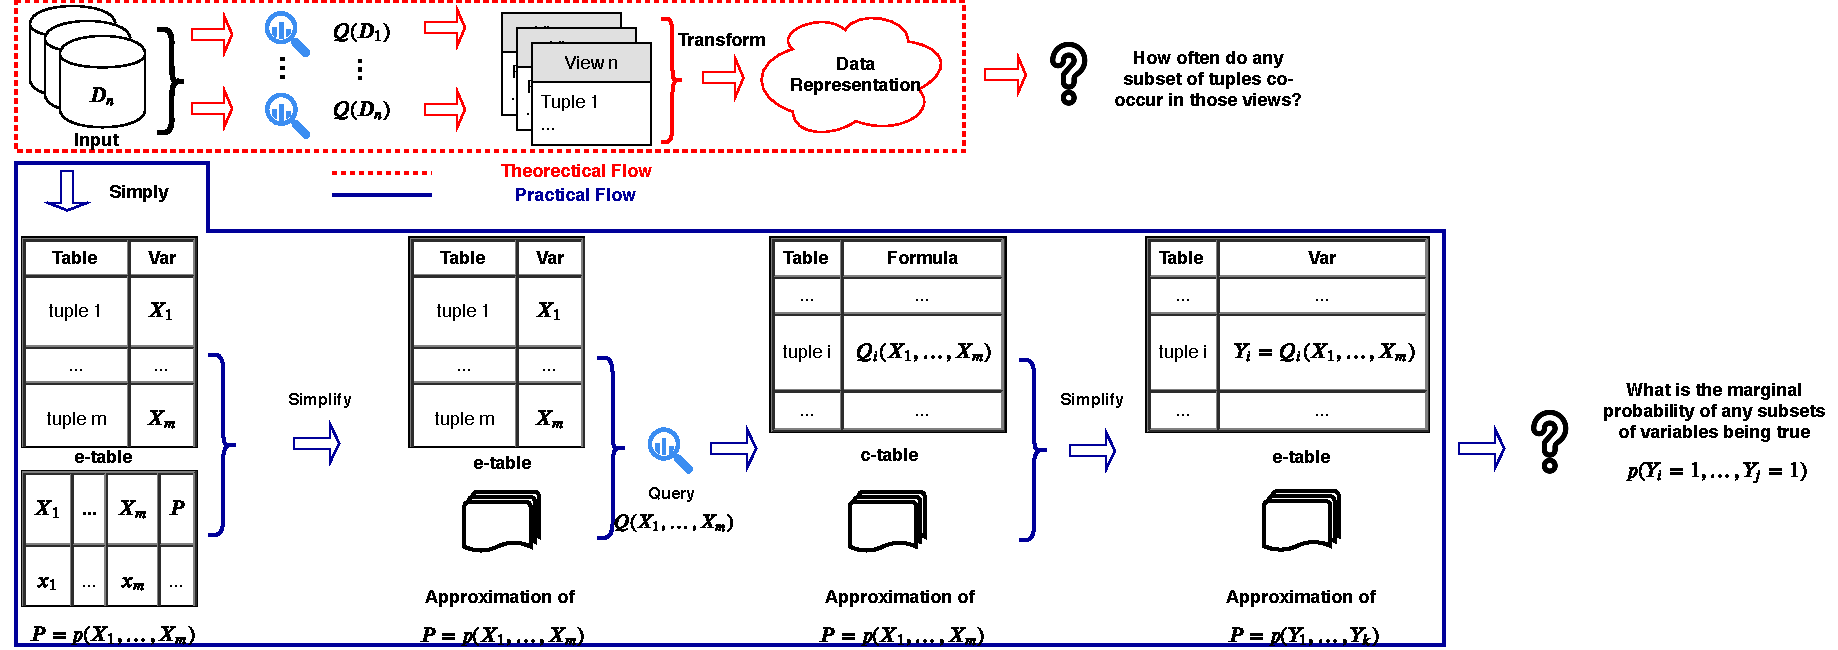
\includegraphics[width=\textwidth]{ProbabilisticDatabaseSummarization/graphics/Data_Flow_Diagram.pdf}
     
 \bfcaption{Theoretical v.s. Practical Data-flows.}
 \label{fig:systemoverview} 
 \trimfigurewhitespace
\end{figure*} 

\subsection{Practical Input Representation}
\label{sec:outputrepresentation}
The previous definition of $\instances$ does not suggest a practical representation, especially when explicit enumeration of all possible worlds is not feasible when $n$ is very large.

\tinysection{C-tables and pc-tables}
We adopt \emph{c-tables} to compactly represent $\instances$. 
A \emph{c-table}~\cite{suciu2009probabilistic} is a set of \emph{distinct} tuples contained in all possible worlds, with each tuple annotated by a propositional formula over random variables.
A \emph{valuation} over these variables assigns each propositional formula a truth value, indicating the existence of the corresponding tuple in a world.
There is a many-to-one mapping from valuations to a possible world.
Extending a c-table by a joint probability distribution over random variables, the resulting \emph{pc-table} can represent any probabilistic database $\probabilisticdatabase$~\cite{suciu2009probabilistic}.

\tinysection{Simplified C-tables}
For our example application, there are two limitations by adopting a general c-table representation.
Firstly, it is difficult to obtain such propositional formula due to lack of knowledge on how tuples are correlated in $\probabilisticdatabase$.
That is, due to complex nature of the function that generates $\probabilisticdatabase$, it is generally hard to formulate how tuples are correlated.
Secondly, the mapping from valuations of variables to possible worlds is many-to-one for a general c-table.
To compute desired marginals, it may require an expensive aggregate over all valuations that map to the same world. 

To overcome the limitations, we represent our input by a family of simplified c-tables, which we call \emph{existence tables} or simply \emph{e-tables}.
Each tuple $\tuplesymbol_i$ in an e-table is annotated with a single random variable $X_i$ whose value is $1$, meaning that the $i$th tuple exists in a world, or $0$ otherwise.
We refer to these variables as \emph{existence variables}.
There is an \emph{one-to-one} mapping from a valuation of existence variables $(x_1,\ldots,x_n)\in\{0,1\}^n$ to a world $\instance$.
The probability of the world (i.e., $\possibleworldsdistribution(\instance)$) can be computed directly from the joint probability distribution $p(X_1=x_1,\ldots,X_n=x_n)$.
When it is clear from context, we abuse notation and denote the distribution $p(X_1=x_1,\ldots,X_n=x_n)$ also as $\possibleworldsdistribution$.
We call an e-table, together with $\possibleworldsdistribution$, a \emph{pe-table}. 

\subsection{Summarizing Joint Distribution}
It is not practical, both in space and marginal computation efficiency, to present pe-table in a view that iterates through all valuations (i.e., worlds) of existence variables.
Hence we need a view that summarizes $\possibleworldsdistribution$ into a more compact form.

\tinysection{Naive Summary}
There can be a set of tuples $\{\ldots,\vec t_i,\ldots\}$ independent of each other such that, 
$$p(\ldots,X_i=1,\ldots)=\Pi_i\;p(X_i=1)$$
In other words, we do not need to store valuations of any combination of those variables in the view, which greatly reduces the number of parameters.
We name the set of parameters $p(X_i=1)$ as a \emph{naive summary} and return to it through out the rest of this paper.
The naive summary is often referred to as \emph{tuple-independent} model~\cite{suciu2009probabilistic}.
When variables are correlated, which is prevalent in our example application, the marginals computed from a naive summary are error-prone.

\tinysection{Loss-less Summary}
For tuples whose variables that are correlated, a \emph{factor graph}~\cite{friedman1999learning} that is equivalent to the marginal probability distribution over these variables, is a sufficient condition for computing any relevant marginals. 
However, it requires heavy weight inference to obtain such set of factors and for each factor, the number of parameters is still exponential to the number of variables that the factor contains.

\tinysection{Lossy Summary}
Practically an application may not require computing exact marginals for \emph{every} set of tuples and we can \emph{cache} marginals that are frequently computed and offer estimation on others. 
Specifically, in our example Entity Resolution task, an application may require to explore labelled tuples that are contained in \emph{all} possible predictions, and tuples that are (in-)frequently or otherwise statistically significant.
The application may tolerate inexact marginal computation for other sets of tuples. 
This observation motivates us to study the option of a \emph{lossy} summary containing only a limited number of marginals and offers estimation on marginals not contained.

\subsection{Pattern-based Summary}

\tinysection{Patterns}
We name a set of co-existing tuples as a \emph{pattern}.
More formally we define a \emph{pattern} as an arbitrary binary vector $\pattern=(x_1,\ldots,x_n)$ with $x_i=1$ meaning the $i$th tuple being present in the pattern.
A pattern $\pattern$ is \emph{contained} in the other $\bar{\pattern}$ if $\forall i, x_i\leq \bar{x}_i$, denoted as $\pattern \subseteq \bar{\pattern}$.
Note that a world $\instance$ is a pattern by definition.
Randomly drawing a world $\instance\in\instances$ from $\probabilisticdatabase$, the probability that it contains pattern $\pattern$ is defined by:
\begin{equation*}
  p(\instances \supseteq \pattern) = \sum_i\possibleworldsdistribution(I_i)\mathbf{1}_{\pattern}(I_i) \;\text{where}\;  \mathbf{1}_{\pattern}(I_i)  =
    \begin{cases}
      1 & \text{if $I_i \supseteq \pattern$}\\
      0 & \text{otherwise}\\
    \end{cases}       
\end{equation*}
In pe-tables, $\marginal$ is equivalent to marginal probability $p(X_1\geq x_1,\ldots,X_n\geq x_n)$.
We call $\marginal$ as the \emph{marginal} of a pattern.

\tinysection{Pattern-based Summary}
Denote the mapping $\encoding_{max}$ from each pattern $\pattern$ to its marginal:
$$\encoding_{max} = \comprehension{\pattern \rightarrow \marginal}{\pattern \in \{0,1\}^n}$$
A \emph{pattern-based summary} $\encoding$ is any such partial mapping $\encoding \subseteq \encoding_{max}$. 
We denote the marginal of pattern $\pattern$ in summary $\encoding$ by $\encoding[\pattern] $ ($= \marginal$).
When it is clear from context, we abuse syntax and also use $\encoding$ to denote the set of patterns it maps (i.e., $domain(\encoding)$).
Hence, $|\encoding|$ is the number of mapped patterns, which we call the summary's \emph{verbosity}.




\section{Marginal Estimation}
A pattern-based summary not only delivers marginals that it contains, but also helps in estimating those that are not explicitly given.

\tinysection{Naive Summary Revisited}
Before detailed explanation, we first consider an intuitive example.
There is one specific family of pattern-based summaries that treat each tuple as being independent, which is equivalent to naive summaries discuss in Section~\ref{sec:outputrepresentation}.
As a re-phrase, we call a pattern-based summary as a naive summary $\naiveencoding$ if it is composed of all patterns that have exactly one possible tuple $\tuplesymbol_i$ with marginal $p(X_i\geq 1)$:
$$domain(\naiveencoding)=\comprehension{(0, \ldots, 0, x_i, 0, \ldots, 0)}{i \in [1,n],\; x_i = 1}$$
To estimate marginals not given in the summary, we apply multiplication $$p(X_1\geq x_1,\ldots,X_n\geq x_n)=\Pi_{i=1,n}\, p(X_i\geq x_i)$$

\tinysection{Patterns as Constraints}
For an arbitrary summary $\encoding$, we characterize its process of marginal computation by defining a \emph{space} (denoted by $\Omega_\encoding$) of distributions $\rho \in \Omega_\encoding$ allowed by a summary $\encoding$.
This space is defined by constraints as follows:
First, we have the general properties of probability distributions:
\begin{center}
$\forall \, \instance_i\in \{0,1\}^n : \rho(\instance_i)\geq 0$
\hspace{10mm}
$\sum_{i=1,2^n}\rho(\instance_i)=1$
\end{center}
Each pattern $\pattern$ in the summary $\encoding$ constrains relevant probabilities in distribution $\rho$ to sum to the target marginal:
\begin{equation*}
\forall \pattern \in domain(\encoding)  :\;\; \encoding[\pattern] = \sum\nolimits_{\instance\supseteq\pattern} \rho(\instance) \;\;\;
\end{equation*}
The dual constraints $1-\encoding[\pattern]=\sum_{\instance\not\supseteq\pattern} \rho(\instance)$ are redundant under the constraint $\sum_i\rho(\instance_i)=1$.

The resulting space $\Omega_\encoding$ is the set of all permitted distributions, or equivalently all input $\probabilisticdatabase$, that obey these constraints.
As a result, the distribution $\rho\in\Omega_\encoding$ that the summary delivers is ambiguous: We model this ambiguity using a random variable $\mathcal P_\encoding$ with support $\Omega_\encoding$.
The true distribution $\possibleworldsdistribution$ must appear in $\Omega_\encoding$, denoted as $\possibleworldsdistribution\equiv\truedistribution\in\Omega_\encoding$ (i.e., $p(\mathcal P_\encoding = \truedistribution) > 0$). 
Of the remaining distributions $\rho$ admitted by $\Omega_\encoding$, it is possible that some are more likely than others.
This prior knowledge may be modeled as a prior on the distribution of $\mathcal P_\encoding$ or equivalently by an additional constraint.
However, for the purposes of this paper, we take the uninformed prior by assuming that $\mathcal P_\encoding$ is uniformly distributed over $\Omega_\encoding$:
\begin{equation*}
\label{uniformprior}
p(\mathcal P_\encoding = \rho) = 
\begin{cases}
\frac{1}{|\Omega_\encoding|} & \text{if } \rho \in \Omega_\encoding\\
0 & \text{otherwise}
\end{cases}
\end{equation*}

The summary delivers marginals by randomly picking one permitted distribution from the entire space and aggregate probabilities accordingly.


\section{Summary Accuracy}
% !TEX root = ../paper.tex
The accuracy of such delivery can be considered from two related, but subtly distinct perspectives:
(1) \emph{Ambiguity} measures how much room the summary leaves for interpretation and 
(2) \emph{Deviation} measures how reliably the summary approximates the target distribution $\truedistribution$.

\smallskip
\tinysection{Ambiguity}
We define the Ambiguity $\ambiguity(\encoding)$ of a summary as the entropy of the random variable $\mathcal P_\encoding$. 
The higher the entropy, the less precisely $\encoding$ identifies a specific distribution.
$$\ambiguity(\encoding) = \mysuml_{\rho}p(\mathcal P_\encoding = \rho)\log \left(p(\mathcal P_\encoding=\rho)\right)$$

\tinysection{Deviation}
The deviation from any permitted distribution $\rho$ to the true distribution $\rho^*$ can be measured by the Kullback-Leibler (K-L) divergence $\mathcal{D}_{KL}(\rho^*||\rho)$.
We define the Deviation $\deviation(\encoding)$ of a summary as the expectation of the K-L divergence over all permitted $\rho \in \Omega_\encoding$:
$$\deviation(\encoding)=\expect_{\mathcal{P}_\encoding}\left[\mathcal{D}_{KL}(\rho^*||\mathcal{P}_\encoding)\right] = \sum_{\rho \in \Omega_\encoding} p(\mathcal P_\encoding = \rho) \cdot \mathcal{D}_{KL}(\rho^*||\rho)$$

\tinysection{Limitations}
Neither Deviation nor Ambiguity has a closed-form formula and it is not practical to enumerate the infinitely large space.
Authors in~\cite{xie2018query} suggests that a single \emph{representative} can be chosen from the space that approximates true distribution $\truedistribution$.

\tinysection{Maximum Entropy Distribution}
The representative distribution is chosen by applying the maximum entropy principle~\cite{DBLP:journals/tssc/Jaynes68} commonly used in pattern-based encoders~\cite{DBLP:journals/tkdd/MampaeyVT12,DBLP:journals/pvldb/GebalyAGKS14}.
That is, we select the distribution $\maximumentropydistribution_{\encoding}$ with maximum entropy:
$$\maximumentropydistribution_{\encoding}=\argmaxl_{\rho\in\Omega_\encoding}\entropy(\rho)\;\;\;\;\;\;\text{where }\entropy(\rho)=\mysuml_{i=[1,2^n]}-\rho(I_i)\log \rho(I_i)$$
The maximum entropy distribution best represents the current state of knowledge.
That is, a distribution with lower entropy assumes additional constraints derived from patterns that we do not know, while one with higher entropy violates the constraints from patterns we do know.

Maximizing an objective function belonging to the exponential family (entropy in our case) under a mixture of linear equality/inequality constraints is a convex optimization problem~\cite{Boyd:2004:CO:993483} which guarantees a \emph{unique} solution and can be solved using the cvx toolkit~\cite{cvx}, and/or by \textit{iterative scaling}~\cite{DBLP:journals/tkdd/MampaeyVT12,DBLP:journals/pvldb/GebalyAGKS14}.

\tinysection{Naive Summary revisited}
For naive summaries $\naiveencoding$ specifically, $\maximumentropydistribution_{\naiveencoding}$ has the closed-form representation:
\begin{equation*}
\maximumentropydistribution_{\naiveencoding}(I)=\prod_{i}p(X_i=x_i)\;\;\;\;\;\;\text{where } I=(x_1,\ldots,x_n)
\end{equation*} 

\tinysection{\Errorname}
We define \emph{\Errorname} $e(\encoding)$ of summary $\encoding$ as the entropy difference between the representative and true distribution:
$$e(\encoding)=\entropy(\overline{\rho}_\encoding)-\entropy(\rho^*)\;\;\;\;\;\text{where }\overline{\rho}_\encoding=\argminl_{\rho\in\Omega_\encoding}-\entropy(\rho)$$
It has been proved~\cite{xie2018query} that \Errorname closely parallels both Ambiguity and Deviation. 

\subsection{Query Accuracy} 
We then study the accuracy of pattern-based summaries when the corresponding probabilistic databases are involved in three basic relational operations: (1) \emph{join}, (2) \emph{selection} and (3) \emph{project}.
Specifically, we study how to modify existing pattern-based summaries in order to suit these operations and give upper-bounds on \Errorname of the resulting summaries.

\subsubsection{Accuracy under join}
Consider two uncertain tables, or equivalently possible worlds $\possibleworldsdistribution_1, \possibleworldsdistribution_2$ under \emph{join} operation.
Recall that possible worlds can be translated into joint distribution, that is, we have $\possibleworldsdistribution_1=p(\ldots,X_i,\ldots)$ and $\possibleworldsdistribution_2=p(\ldots,Y_j,\ldots)$ where $X_i,Y_j$ indicate the presence of $i,j$th tuple in possible worlds $\possibleworldsdistribution_1,\possibleworldsdistribution_2$ respectively.
The resulting uncertain table after \emph{join}, or equivalently possible worlds $\possibleworldsdistribution_{1\times 2}=\possibleworldsdistribution_1\times\possibleworldsdistribution_2$ can also be translated into joint distribution $\possibleworldsdistribution_{1\times 2}=p(\ldots,Z_{i,j},\ldots)$ where $Z_{i,j}=1$ iff $X_i=1$ and $Y_j=1$.

\tinysection{Join-derived summary}
Consider pattern-based summaries $\encoding_1, \encoding_2$ for $\possibleworldsdistribution_1,\possibleworldsdistribution_2$ with corresponding maximum entropy distribution $\maximumentropydistribution_{\encoding_1},\maximumentropydistribution_{\encoding_2}$.
The resulting summary $\encoding_{1\times2}$ can be obtained from \emph{joining} patterns from both summaries and multiplying their corresponding marginals.
Denote the resulting maximum entropy distribution after \emph{join} as $\maximumentropydistribution_{\encoding_{1\times 2}}$.

\tinysection{Upper-bound of \Errorname}
By definition, the \Errorname $e(\encoding_{1\times 2})$ of summary $\encoding_{1\times 2}$ measures the entropy difference $\entropy(\maximumentropydistribution_{\encoding_{1\times 2}})-\entropy(\possibleworldsdistribution_{1\times 2})$.
We would like to approximate the two entropies to avoid populating mappings in distributions $\maximumentropydistribution_{\encoding_{1\times 2}}$ and $\possibleworldsdistribution_{1\times 2}$.
That is, we would like to provide an upper-bound $\tilde{e}(\encoding_{1\times 2})$ and such that $e(\encoding_{1\times 2})\leq \tilde{e}(\encoding_{1\times 2})$.

Observe that there is a many-to-one mapping from valuations of jointly distributed variables $\possibleworldsdistribution_{1,2}=p(\ldots,X_i,\ldots,Y_j,\ldots)$ to $\possibleworldsdistribution_{1\times 2}$.
That is, by fixing the valuation of all other variables except for some pair $X_i,Y_j$, all three cases where $X_i=0 \land Y_j=0$, $X_i=0 \land Y_j=1$ or $X_i=1 \land Y_j=0$ map to the same valuation of $\possibleworldsdistribution_{1\times 2}$ where $Z_{i,j}=0$.
Hence, the entropy $\entropy(\possibleworldsdistribution_{1\times 2})\leq \entropy(\possibleworldsdistribution_{1,2})$.
Trivially we also have $\entropy(\possibleworldsdistribution_{1\times 2})\geq \max(\entropy(\possibleworldsdistribution_1),\entropy(\possibleworldsdistribution_2))$.
Since $X_i$ are independent of $Y_j$ in $\possibleworldsdistribution_{1,2}$, we have $\entropy(\possibleworldsdistribution_{1,2})=\entropy(\possibleworldsdistribution_1)+\entropy(\possibleworldsdistribution_2)$.
We have similar observation for maximum entropy distributions: $\entropy(\maximumentropydistribution_{\encoding_{1\times 2}}) \leq \entropy(\maximumentropydistribution_{\encoding_1})+\entropy(\maximumentropydistribution_{\encoding_2})$.
We thus compute the upper-bound $\tilde{e}(\encoding_{1\times 2})=\entropy(\maximumentropydistribution_{\encoding_1})+\entropy(\maximumentropydistribution_{\encoding_2})-\max(\entropy(\possibleworldsdistribution_1),\entropy(\possibleworldsdistribution_2))$ or a looser but simpler bound $\entropy(\maximumentropydistribution_{\encoding_1})+\entropy(\maximumentropydistribution_{\encoding_2})$.

\subsubsection{Accuracy under selection predicate}
Consider the case where only a subset of tuples in possible worlds $\possibleworldsdistribution=p(\ldots,X_i,\ldots)$ are chosen, according to some arbitrary \emph{selection} predicate $\sigma$. 
For convenience, we abuse notation and also represent the indices of its chosen tuples as $\sigma$.
The resulting possible worlds, or equivalently the joint distribution $\possibleworldsdistribution_{\sigma}$ is the marginal distribution $p(\ldots,X_{i\in\sigma},\ldots)$ by summing out variables $X_{i\not\in\sigma}$.

\tinysection{Selection-derived summary}
Consider a pattern-based summary $\encoding$ for $\possibleworldsdistribution$, the resulting summary $\encoding_{\sigma}$ for $\possibleworldsdistribution_{\sigma}$ can be constructed in three steps: (1) remove tuples that are not chosen by $\sigma$ for each pattern in $\encoding$, (2) merge patterns that are the same and add their marginals and (3) remove empty patterns.

\tinysection{Upper-bound of \Errorname}
Suppose we encode $\possibleworldsdistribution$ first by naive summary $\naiveencoding$ whose maximum entropy distribution $\maximumentropydistribution_{\naiveencoding}$ is equivalent to tuple-independent model.
The resulting naive summary $\naiveencoding_{\sigma}\subseteq \naiveencoding$ after \emph{select} operation is a subset of single-tuple patterns filtered by the predicate $\sigma$. 
\Errorname of the naive summary $\naiveencoding_{\sigma}$ is thus computed as $e(\naiveencoding_{\sigma})=\sum_{i\in\sigma} \entropy\big(p(X_i)\big)-\entropy(\possibleworldsdistribution_{\sigma})$.
In cases when we do not want to populate mappings of distribution $\possibleworldsdistribution_{\sigma}$ for each given predicate, we can simply compute $\tilde{e}(\naiveencoding_{\sigma})=\sum_{i\in\sigma} \entropy\big(p(X_i)\big)$ which is the upper-bound of $e(\naiveencoding_{\sigma})$ for all possible $\sigma$.
For any other summary $\encoding_{\sigma}$ that contains naive summary $\encoding_{\sigma}\supseteq \naiveencoding_{\sigma}$, it may improve naive summary by marginals that encode tuple-correlation.
Hence the \Errorname $e(\encoding_{\sigma})$ is also upper-bounded by $\tilde{e}(\naiveencoding_{\sigma})$.
Trivially, we also have $e(\encoding_{\sigma})\leq \entropy(\maximumentropydistribution_{\encoding})$.
Hence the \Errorname of any summary $\encoding_{\sigma}\supseteq\naiveencoding_{\sigma}$ is upper-bounded by $\min\big(\tilde{e}(\naiveencoding_{\sigma}),\entropy(\maximumentropydistribution_{\encoding})\big)$.

\subsubsection{Accuracy under project}
Consider the case where tuples in uncertain table $\possibleworldsdistribution$ are \emph{projected} onto an arbitrary set of attributes $A$.
We group tuples whose values are the same on projected attributes $A$ and create a new random variable $Z$ for each group, where $Z=0$ iff $X_i=0$ for all tuples $\tuplesymbol_i$ in the group, otherwise $Z=1$.
The possible worlds distribution $\possibleworldsdistribution_{\pi_A}$ after \emph{project} operation, is thus the joint distribution $p(Z_1,\ldots,Z_k)$ where $k$ is the total number of tuple groups.

\tinysection{Project-derived summary}
Suppose we have summary $\encoding$ for $\possibleworldsdistribution$. 
The resulting summary $\encoding_{\pi_A}$ for $\possibleworldsdistribution_{\pi_A}$ can be constructed by (1) applying \emph{project} on each pattern and (2) merge patterns that are the same after \emph{project} and add their marginals accordingly.

\tinysection{Upper-bound of \Errorname}
We fix the valuations for all $Z_i$ except for the $k$th group $Z_k$.
Equivalently we fix all valuations of $X_i$ in $\possibleworldsdistribution$ except for those $X_j$ that belong to $k$th group.
Then we notice that there is a many-to-one mapping from all valuations of $X_j$ in the group, where at least one $X_j=1$, to $Z_k=1$.
In other words, we have $\entropy(\possibleworldsdistribution_{\pi_A})\leq \entropy(\possibleworldsdistribution)$.
Similarly we also have $\entropy(\maximumentropydistribution_{\encoding_{\pi_A}})\leq \entropy(\maximumentropydistribution_{\encoding})$ for maximum entropy distributions of corresponding summaries.
That is, the \Errorname of summary $\encoding_{\pi_A}$ for any \emph{project} operation $\pi_A$ is upper-bounded by $\entropy(\maximumentropydistribution_{\encoding})-\entropy(\possibleworldsdistribution_{\pi_A})$ or a looser but simpler bound $\entropy(\maximumentropydistribution_{\encoding})$.



\section{Constructing Summaries}
%\input{ProbabilisticDatabaseSummarization/sections/6-LossBounds.tex}

%\section{Related Work}
%% !TEX root = ../paper.tex
\label{sec:relatedwork}
In this section, we walk through related work on encoding tuple correlation in probabilistic databases using various kinds of auxiliary information.

\tinysection{C-tables}
The canonical representation of probabilistic databases is \emph{c-table}~\cite{suciu2009probabilistic}.
A \emph{c-table} is a table with each tuple annotated with an additional attribute: a propositional formula over random variables. 
Two tuples are correlated if random variables in their propositional formula depends on each other.
Given a query over a c-table, the correlation among tuples in the query answer is encoded by the \emph{lineage} (or provenance~\cite{cui2003lineage}) of each tuple, which is also a propositional formula.

Based on c-tables, Trio system~\cite{benjelloun2006uldbs} resolves tuple correlation by tracking lineage of tuples in query processing.
By defining a probability space over the assignments of the random variables in lineage of tuples, a \emph{confidence value} can be computed for each tuple in the query answer.
The probability of some answer to be chosen as the "correct" one is proportional to the product of confidence values of all of its tuples.
Similar idea can be found in MayBMS~\cite{Huang:2009:MPD:1559845.1559984}.
However, as ~\cite{re2007materialized} pointed out, there are cases where lineage is not obtainable.
In our example application, tuples are correlated in a latent, complex way that populating propositional formula for tuples in the c-table is difficult.  

\tinysection{Graphical models and Factors}
Enlightened by Probablistic Relational Model (PRM)~\cite{friedman1999learning}, numerous works~~\cite{sen2007representing, sen2009prdb} use \emph{probabilistic graphical models} (PGM) to encode tuple correlation directly by probabilities of co-existing tuples.
More specifically, considering any set of co-existing tuples, encoded as a binary vector $\vec v=(x_1,\ldots,x_n)$ with $x_i=1$ indicating the presence of the $i$th possible tuple in the co-existence relationship.
A \emph{factor function} or simply \emph{factor} $f: \vec v\in\{0,1\}^n \to [0,1]$ maps any set of co-existing tuples $\vec v$ to its probability of being present in the probabilistic database. 
Since there are exponentially large (i.e., $2^n$) number of mappings, instead of having a single factor that takes $n$ variables as input, we can have multiple factors, each takes only a small subset of variables that are correlated.
If two factors do not share variables, the variables in one are considered independent of those in the other.
By multiplying the outputs of the two factors, we can efficiently compute the probability of any combination of variables in two factors. 

\tinysection{Markov Logic Networks}
Jha and Suciu~\cite{jha2012probabilistic} shows how to automatically generate factors and populate their content mappings using prior knowledge on tuple-correlation, expressed by the language of First Order Logic.
Similar technique is implemented in DeepDive system~\cite{shin2015incremental}.

As authors of MCDB~\cite{jampani2008mcdb} pointed out, most previously discussed approaches augment data with attribute-level or tuple-level annotations, which are loaded into the database along with the data itself.
The mixture of data and uncertainty annotation is inflexible when changes have to be made to the underlying uncertainty model (e.g., lineage), as all related annotations typically need to be recomputed outside of the database and then loaded back in.
To facilitate maintenance, MCDB proposes to separate uncertainty model from the data.

\tinysection{Monte Carlo approach}
More specifically, MCDB allows a user to define arbitrary \emph{variable generation} (VG) functions that encodes the uncertainty model.
That is, treating a VG function as a black box, MCDB use it to pseudo-randomly generate samples of possible instances on the fly and run queries over the samples.
Interestingly, sample instances are sets of co-existing tuples.
By assigning a probability to each sample, the probability of any co-existing tuples that are contained in any sample is estimated naturally by iterating through the samples. 


%%%%%%%%%%%%%%%%%%%%%%%%%%%%%%%%%%%%%%%%%%%%%%%%%%%%%%%%%%%%%%%
% ESM students need to include a Nontechnical Abstract as the %
% last appendix.                                              %
%%%%%%%%%%%%%%%%%%%%%%%%%%%%%%%%%%%%%%%%%%%%%%%%%%%%%%%%%%%%%%%
% This \include command should point to the file containing
% that abstract.
%\include{nontechnical-abstract}
%%%%%%%%%%%%%%%%%%%%%%%%%%%%%%%%%%%%%%%%%%%
} % End of the \allowdisplaybreak command %
%%%%%%%%%%%%%%%%%%%%%%%%%%%%%%%%%%%%%%%%%%%

%%%%%%%%%%%%%%%%
% BIBLIOGRAPHY %
%%%%%%%%%%%%%%%%
% You can use BibTeX or other bibliography facility for your
% bibliography. LaTeX's standard stuff is shown below. If you
% bibtex, then this section should look something like:
   \begin{singlespace}
   \bibliographystyle{unsrt}
   \phantomsection \addcontentsline{toc}{chapter}{Bibliography}
   \bibliography{ref}
   \end{singlespace}

%\begin{singlespace}
%\begin{thebibliography}{99}
%\addcontentsline{toc}{chapter}{Bibliography}
%\frenchspacing

%\bibitem{Wisdom87} J. Wisdom, ``Rotational Dynamics of Irregularly Shaped Natural Satellites,'' \emph{The Astronomical Journal}, Vol.~94, No.~5, 1987  pp. 1350--1360.

%\bibitem{G&H83} J. Guckenheimer and P. Holmes, \emph{Nonlinear Oscillations, Dynamical Systems, and Bifurcations of Vector Fields}, Springer-Verlag, New York, 1983.

%\end{thebibliography}
%\end{singlespace}

\backmatter

% Vita
% \vita{SupplementaryMaterial/Vita}

\end{document}

